% Generated by Sphinx.
\def\sphinxdocclass{report}
\documentclass[A4paper,10pt,icelandic]{sphinxmanual}
\usepackage[utf8]{inputenc}
\DeclareUnicodeCharacter{00A0}{\nobreakspace}
\usepackage{cmap}
\usepackage{amsmath}
\usepackage{amssymb}
%\usepackage{hyperref}
\usepackage[T1]{fontenc}
\usepackage{babel}
\usepackage{times}
\usepackage[Sonny]{fncychap}
\usepackage{longtable}
\usepackage{sphinx}
\usepackage{multirow}


\title{Töluleg greining (STÆ405G)}
\date{January 23, 2016}
\release{0.1}
\author{Benedikt Steinar Magnússon}
\newcommand{\sphinxlogo}{
\includegraphics{hi_vnvs_horiz_raunvisindadeild.jpg}\par}
\renewcommand{\releasename}{Útgáfa}
\makeindex

\makeatletter
\def\PYG@reset{\let\PYG@it=\relax \let\PYG@bf=\relax%
    \let\PYG@ul=\relax \let\PYG@tc=\relax%
    \let\PYG@bc=\relax \let\PYG@ff=\relax}
\def\PYG@tok#1{\csname PYG@tok@#1\endcsname}
\def\PYG@toks#1+{\ifx\relax#1\empty\else%
    \PYG@tok{#1}\expandafter\PYG@toks\fi}
\def\PYG@do#1{\PYG@bc{\PYG@tc{\PYG@ul{%
    \PYG@it{\PYG@bf{\PYG@ff{#1}}}}}}}
\def\PYG#1#2{\PYG@reset\PYG@toks#1+\relax+\PYG@do{#2}}

\expandafter\def\csname PYG@tok@gr\endcsname{\def\PYG@tc##1{\textcolor[rgb]{1.00,0.00,0.00}{##1}}}
\expandafter\def\csname PYG@tok@s1\endcsname{\def\PYG@tc##1{\textcolor[rgb]{0.25,0.44,0.63}{##1}}}
\expandafter\def\csname PYG@tok@no\endcsname{\def\PYG@tc##1{\textcolor[rgb]{0.38,0.68,0.84}{##1}}}
\expandafter\def\csname PYG@tok@vi\endcsname{\def\PYG@tc##1{\textcolor[rgb]{0.73,0.38,0.84}{##1}}}
\expandafter\def\csname PYG@tok@c1\endcsname{\let\PYG@it=\textit\def\PYG@tc##1{\textcolor[rgb]{0.25,0.50,0.56}{##1}}}
\expandafter\def\csname PYG@tok@sx\endcsname{\def\PYG@tc##1{\textcolor[rgb]{0.78,0.36,0.04}{##1}}}
\expandafter\def\csname PYG@tok@gd\endcsname{\def\PYG@tc##1{\textcolor[rgb]{0.63,0.00,0.00}{##1}}}
\expandafter\def\csname PYG@tok@nf\endcsname{\def\PYG@tc##1{\textcolor[rgb]{0.02,0.16,0.49}{##1}}}
\expandafter\def\csname PYG@tok@ss\endcsname{\def\PYG@tc##1{\textcolor[rgb]{0.32,0.47,0.09}{##1}}}
\expandafter\def\csname PYG@tok@nd\endcsname{\let\PYG@bf=\textbf\def\PYG@tc##1{\textcolor[rgb]{0.33,0.33,0.33}{##1}}}
\expandafter\def\csname PYG@tok@vc\endcsname{\def\PYG@tc##1{\textcolor[rgb]{0.73,0.38,0.84}{##1}}}
\expandafter\def\csname PYG@tok@si\endcsname{\let\PYG@it=\textit\def\PYG@tc##1{\textcolor[rgb]{0.44,0.63,0.82}{##1}}}
\expandafter\def\csname PYG@tok@nn\endcsname{\let\PYG@bf=\textbf\def\PYG@tc##1{\textcolor[rgb]{0.05,0.52,0.71}{##1}}}
\expandafter\def\csname PYG@tok@gh\endcsname{\let\PYG@bf=\textbf\def\PYG@tc##1{\textcolor[rgb]{0.00,0.00,0.50}{##1}}}
\expandafter\def\csname PYG@tok@kt\endcsname{\def\PYG@tc##1{\textcolor[rgb]{0.56,0.13,0.00}{##1}}}
\expandafter\def\csname PYG@tok@ge\endcsname{\let\PYG@it=\textit}
\expandafter\def\csname PYG@tok@bp\endcsname{\def\PYG@tc##1{\textcolor[rgb]{0.00,0.44,0.13}{##1}}}
\expandafter\def\csname PYG@tok@mo\endcsname{\def\PYG@tc##1{\textcolor[rgb]{0.13,0.50,0.31}{##1}}}
\expandafter\def\csname PYG@tok@mf\endcsname{\def\PYG@tc##1{\textcolor[rgb]{0.13,0.50,0.31}{##1}}}
\expandafter\def\csname PYG@tok@sb\endcsname{\def\PYG@tc##1{\textcolor[rgb]{0.25,0.44,0.63}{##1}}}
\expandafter\def\csname PYG@tok@nv\endcsname{\def\PYG@tc##1{\textcolor[rgb]{0.73,0.38,0.84}{##1}}}
\expandafter\def\csname PYG@tok@k\endcsname{\let\PYG@bf=\textbf\def\PYG@tc##1{\textcolor[rgb]{0.00,0.44,0.13}{##1}}}
\expandafter\def\csname PYG@tok@sr\endcsname{\def\PYG@tc##1{\textcolor[rgb]{0.14,0.33,0.53}{##1}}}
\expandafter\def\csname PYG@tok@err\endcsname{\def\PYG@bc##1{\setlength{\fboxsep}{0pt}\fcolorbox[rgb]{1.00,0.00,0.00}{1,1,1}{\strut ##1}}}
\expandafter\def\csname PYG@tok@cm\endcsname{\let\PYG@it=\textit\def\PYG@tc##1{\textcolor[rgb]{0.25,0.50,0.56}{##1}}}
\expandafter\def\csname PYG@tok@nl\endcsname{\let\PYG@bf=\textbf\def\PYG@tc##1{\textcolor[rgb]{0.00,0.13,0.44}{##1}}}
\expandafter\def\csname PYG@tok@kp\endcsname{\def\PYG@tc##1{\textcolor[rgb]{0.00,0.44,0.13}{##1}}}
\expandafter\def\csname PYG@tok@sd\endcsname{\let\PYG@it=\textit\def\PYG@tc##1{\textcolor[rgb]{0.25,0.44,0.63}{##1}}}
\expandafter\def\csname PYG@tok@kn\endcsname{\let\PYG@bf=\textbf\def\PYG@tc##1{\textcolor[rgb]{0.00,0.44,0.13}{##1}}}
\expandafter\def\csname PYG@tok@kr\endcsname{\let\PYG@bf=\textbf\def\PYG@tc##1{\textcolor[rgb]{0.00,0.44,0.13}{##1}}}
\expandafter\def\csname PYG@tok@se\endcsname{\let\PYG@bf=\textbf\def\PYG@tc##1{\textcolor[rgb]{0.25,0.44,0.63}{##1}}}
\expandafter\def\csname PYG@tok@il\endcsname{\def\PYG@tc##1{\textcolor[rgb]{0.13,0.50,0.31}{##1}}}
\expandafter\def\csname PYG@tok@s\endcsname{\def\PYG@tc##1{\textcolor[rgb]{0.25,0.44,0.63}{##1}}}
\expandafter\def\csname PYG@tok@na\endcsname{\def\PYG@tc##1{\textcolor[rgb]{0.25,0.44,0.63}{##1}}}
\expandafter\def\csname PYG@tok@gi\endcsname{\def\PYG@tc##1{\textcolor[rgb]{0.00,0.63,0.00}{##1}}}
\expandafter\def\csname PYG@tok@s2\endcsname{\def\PYG@tc##1{\textcolor[rgb]{0.25,0.44,0.63}{##1}}}
\expandafter\def\csname PYG@tok@gt\endcsname{\def\PYG@tc##1{\textcolor[rgb]{0.00,0.27,0.87}{##1}}}
\expandafter\def\csname PYG@tok@w\endcsname{\def\PYG@tc##1{\textcolor[rgb]{0.73,0.73,0.73}{##1}}}
\expandafter\def\csname PYG@tok@mi\endcsname{\def\PYG@tc##1{\textcolor[rgb]{0.13,0.50,0.31}{##1}}}
\expandafter\def\csname PYG@tok@gu\endcsname{\let\PYG@bf=\textbf\def\PYG@tc##1{\textcolor[rgb]{0.50,0.00,0.50}{##1}}}
\expandafter\def\csname PYG@tok@mb\endcsname{\def\PYG@tc##1{\textcolor[rgb]{0.13,0.50,0.31}{##1}}}
\expandafter\def\csname PYG@tok@cp\endcsname{\def\PYG@tc##1{\textcolor[rgb]{0.00,0.44,0.13}{##1}}}
\expandafter\def\csname PYG@tok@vg\endcsname{\def\PYG@tc##1{\textcolor[rgb]{0.73,0.38,0.84}{##1}}}
\expandafter\def\csname PYG@tok@c\endcsname{\let\PYG@it=\textit\def\PYG@tc##1{\textcolor[rgb]{0.25,0.50,0.56}{##1}}}
\expandafter\def\csname PYG@tok@gs\endcsname{\let\PYG@bf=\textbf}
\expandafter\def\csname PYG@tok@nc\endcsname{\let\PYG@bf=\textbf\def\PYG@tc##1{\textcolor[rgb]{0.05,0.52,0.71}{##1}}}
\expandafter\def\csname PYG@tok@nt\endcsname{\let\PYG@bf=\textbf\def\PYG@tc##1{\textcolor[rgb]{0.02,0.16,0.45}{##1}}}
\expandafter\def\csname PYG@tok@sh\endcsname{\def\PYG@tc##1{\textcolor[rgb]{0.25,0.44,0.63}{##1}}}
\expandafter\def\csname PYG@tok@kc\endcsname{\let\PYG@bf=\textbf\def\PYG@tc##1{\textcolor[rgb]{0.00,0.44,0.13}{##1}}}
\expandafter\def\csname PYG@tok@m\endcsname{\def\PYG@tc##1{\textcolor[rgb]{0.13,0.50,0.31}{##1}}}
\expandafter\def\csname PYG@tok@kd\endcsname{\let\PYG@bf=\textbf\def\PYG@tc##1{\textcolor[rgb]{0.00,0.44,0.13}{##1}}}
\expandafter\def\csname PYG@tok@ne\endcsname{\def\PYG@tc##1{\textcolor[rgb]{0.00,0.44,0.13}{##1}}}
\expandafter\def\csname PYG@tok@gp\endcsname{\let\PYG@bf=\textbf\def\PYG@tc##1{\textcolor[rgb]{0.78,0.36,0.04}{##1}}}
\expandafter\def\csname PYG@tok@cs\endcsname{\def\PYG@tc##1{\textcolor[rgb]{0.25,0.50,0.56}{##1}}\def\PYG@bc##1{\setlength{\fboxsep}{0pt}\colorbox[rgb]{1.00,0.94,0.94}{\strut ##1}}}
\expandafter\def\csname PYG@tok@o\endcsname{\def\PYG@tc##1{\textcolor[rgb]{0.40,0.40,0.40}{##1}}}
\expandafter\def\csname PYG@tok@ni\endcsname{\let\PYG@bf=\textbf\def\PYG@tc##1{\textcolor[rgb]{0.84,0.33,0.22}{##1}}}
\expandafter\def\csname PYG@tok@ow\endcsname{\let\PYG@bf=\textbf\def\PYG@tc##1{\textcolor[rgb]{0.00,0.44,0.13}{##1}}}
\expandafter\def\csname PYG@tok@sc\endcsname{\def\PYG@tc##1{\textcolor[rgb]{0.25,0.44,0.63}{##1}}}
\expandafter\def\csname PYG@tok@mh\endcsname{\def\PYG@tc##1{\textcolor[rgb]{0.13,0.50,0.31}{##1}}}
\expandafter\def\csname PYG@tok@go\endcsname{\def\PYG@tc##1{\textcolor[rgb]{0.20,0.20,0.20}{##1}}}
\expandafter\def\csname PYG@tok@nb\endcsname{\def\PYG@tc##1{\textcolor[rgb]{0.00,0.44,0.13}{##1}}}

\def\PYGZbs{\char`\\}
\def\PYGZus{\char`\_}
\def\PYGZob{\char`\{}
\def\PYGZcb{\char`\}}
\def\PYGZca{\char`\^}
\def\PYGZam{\char`\&}
\def\PYGZlt{\char`\<}
\def\PYGZgt{\char`\>}
\def\PYGZsh{\char`\#}
\def\PYGZpc{\char`\%}
\def\PYGZdl{\char`\$}
\def\PYGZhy{\char`\-}
\def\PYGZsq{\char`\'}
\def\PYGZdq{\char`\"}
\def\PYGZti{\char`\~}
% for compatibility with earlier versions
\def\PYGZat{@}
\def\PYGZlb{[}
\def\PYGZrb{]}
\makeatother

\renewcommand\PYGZsq{\textquotesingle}

\begin{document}

\maketitle
\tableofcontents
\phantomsection\label{index::doc}



\chapter{Inngangur}
\label{kafli01::doc}\label{kafli01:inngangur}
\emph{He was determined to discover the underlying logic behind the universe. Which was going to be hard, because there wasn't one.}

- Terry Pratchett, Mort


\section{Hvað er töluleg greining?}
\label{kafli01:hva-er-toluleg-greining}

\subsection{Tilraun að svari}
\label{kafli01:tilraun-a-svari}\begin{itemize}
\item {} 
Fagið \emph{töluleg greining} snýst um að búa til, greina og forrita
aðferðir til þess að nálga á lausnum á stærðfræðilegum verkefnum.

\item {} 
Aðferðirnar eru settar fram með reikniritum sem síðan eru forrituð og
það þarf góðan skilning á eiginleikum lausnanna sem verið er að nálga
til þess að geta greint hvernig forritin munu virka.

\item {} 
Greining á reikniritum er aðallega fólgin í skekkjumati og mati á
þeim aðgerðafjölda sem þarf til þess að ná að nálga lausn með
fyrirfram gefinni nákvæmni, þ.e. hagkvæmni og nákvæmni reikniritsins.

\item {} 
Líkanagerð í raunvísindum og verkfræði felur yfirleitt í sér eftirfarandi skref:
\begin{enumerate}
\item {} 
\emph{Greina} kerfið sem um ræðir

\item {} 
\emph{Smíða líkan} sem útskýrir hvernig kerfið hegðar sér, þó yfirleitt með töluverðum einföldunum.

\item {} 
\emph{Herma} kerfið í tölvu eins vel og hægt er. Hér þarf að ná ásættanlegri námkvæmni á þeim tíma sem útreikningar mega taka.

\item {} 
\emph{Túlka} niðurstöðurnar og bera saman við upphaflega kerfið.

\end{enumerate}

Töluleg greining kemur mikið við sögu í lið 3. og einnig í lið 4.

\end{itemize}


\section{Dæmi: Eldflaug}
\label{kafli01:daemi-eldflaug}
Gerum ráð fyrir að við höfum eftirfarandi eldflaug undir höndum:
\begin{itemize}
\item {} 
Eldsneytið dugir í 18 sek., þ.e. \(t\in [0,18]\).

\item {} 
Loftmótstaðan er \(d=0.1v^2\), þar sem \(v(t)\) er hraðinn á tíma \(t\).

\item {} 
Krafturinn sem knýr flaugina er \(T=5000\) N.

\item {} 
Massi eldsneytisins er \(m=180-10t\) kg.

\item {} 
Massi flaugarinnar er \(M = 120 + m = 300 - 10t\) kg.

\end{itemize}

Spurningin er: Í hvaða hæð er eldflaugin þegar eldsneytið klárast?

Úr öðru lögmáli Newtons fæst að \(F = (Mv)'\). Kraftarnir sem verka
á eldflaugina er \(T\) upp á við og loftmótstaðan og
þyngdarkrafturinn niður á við. Þannig fæst
\begin{gather}
\begin{split}(Mv)' = F = T - Mg - d\end{split}\notag
\end{gather}
það er
\begin{gather}
\begin{split}M'v + Mv' = T - Mg -d.\end{split}\notag
\end{gather}
Þetta jafngildir því að
\phantomsection\label{kafli01:eldflaug}\begin{gather}
\begin{split}v' = \frac{T-Mg-d-M'v}{M} = \frac{5000-(300-10t)g-0,1v^2+10v}{300-10t},
\label{eldflaug}\end{split}\notag
\end{gather}
og upphafsskilyrðin eru \(v(0) =0\).

Þar sem \(h' = v\), þá er hæðin á tíma \(t\) gefin með
\(h(t) =\int_0^t v(s)\, ds\). Þegar eldsneytið klárast þá er hæðin
\(h(18) = \int_0^{18} v(s)\, ds\).

Verkefnið er því að finna \(v\), og reikna svo heildið.

{\hyperref[kafli01:eldflaug]{\emph{Diffurjafnan}}} hér að ofan er ólínuleg og ekki aðgreinanleg þannig
að við getum ekki vænst
þess finna lausn með þeim aðferðum sem við höfum þegar lært. Eins er
ekki víst að við getum auðveldlega fundið stofnfall \(h\) fyrir
\(v\) til þess að reikna heildið, jafnvel þótt við hefðum \(v\).

Hins vegar getum við leyst diffurjöfnuna tölulega með aðferðunum úr
{\hyperref[kafli06:upphafsgildisverkefni]{\emph{kafla 6}}},
og heildið reiknum við svo tölulega með aðferðunum úr {\hyperref[kafli05:heildun]{\emph{kafla 5}}}.


\section{Samleitni runa}
\label{kafli01:samleitni-runa}

\subsection{Nokkur atriði um samleitni runa}
\label{kafli01:nokkur-atrii-um-samleitni-runa}
Mörg reiknirit til nálgunar á einhverri rauntölu eru hönnuð þannig að
reiknuð er runa \(x_0,x_1,x_2,\dots\) sem á að nálgast lausnina
okkar.

\index{runa}\index{samleitni}\index{samleitni!línuleg}\index{samleitni!ofurlínuleg}\index{samleitni!ferningssamleitni}\index{samleitni!af stigi \(\alpha\)}\index{markgildi}

\subsection{Skilgreining: Samleitni}
\label{kafli01:skilgreining-samleitni}\label{kafli01:index-0}
\emph{Rauntalnaruna} \((x_n)\) er sögð vera \emph{samleitin} (e. convergent)
að \emph{markgildinu} \(r\) ef um sérhvert \(\varepsilon>0\) gildir
að til er \(N>0\) þannig að
\begin{gather}
\begin{split}|x_n-r|<\varepsilon, \qquad \text{ ef } \quad n\geq N.\end{split}\notag
\end{gather}
Þetta er táknað annað hvort með
\begin{gather}
\begin{split}\lim_{n\to \infty}x_n=r \qquad \text{ eða } \qquad  x_n\to r
    \text{ ef } n\to \infty.\end{split}\notag
\end{gather}
Ef runan \((x_n)\) er samleitin að markgildinu \(r\) þá segjum
við einnig að hún \emph{stefni á} \(r\).

Hugsum okkur nú að \((x_n)\) sé gefin runa sem stefnir á \(r\)
og táknum skekkjuna með \(e_n=r-x_n\).

Runan er sögð vera \emph{línulega samleitin} (e. linear convergence) ef til
er \(\lambda\in ]0,1[\) þannig að
\begin{gather}
\begin{split}\lim_{n\to \infty}\dfrac{|e_{n+1}|}{|e_n|}=\lambda,\end{split}\notag
\end{gather}
\emph{ofurlínulega samleitin} (e. superlinear convergence), ef
\begin{gather}
\begin{split}\lim_{n\to \infty}\dfrac{|e_{n+1}|}{|e_n|}=0,\end{split}\notag
\end{gather}
\emph{ferningssamleitin} (e. quadratic convergence) ef til er \(\lambda>0\) þannig að
\begin{gather}
\begin{split}\lim_{n\to \infty}\dfrac{|e_{n+1}|}{|e_n|^2}=\lambda,\end{split}\notag
\end{gather}
og \emph{samleitin af stigi} \(\alpha\) (e. convergence of order
\(\alpha\)), þar sem \(\alpha> 1\), ef til er \(\lambda>0\)
þannig að
\begin{gather}
\begin{split}\lim_{n\to \infty}\dfrac{|e_{n+1}|}{|e_n|^\alpha}=\lambda.\end{split}\notag
\end{gather}
\begin{notice}{note}{Athugasemd:}
Runa er ofurlínulega samleitin ef hún er samleitin af stigi \(\alpha>1\).

Ferningssamleitin runa er samleitin af stigi 2 þannig að hún er einnig ofurlínulega samleitin.
\end{notice}


\subsection{Skilgreining}
\label{kafli01:skilgreining}
Oft eru notuð veikari hugtök til þess að lýsa samleitni runa (t.d. ef
við getum ekki fundið \(\lambda\) og \(\alpha\) nákvæmlega).

Þannig segjum við að runan \((x_n)\) sé \emph{að minnsta kosti línulega
samleitin} ef til er \(\lambda\in ]0,1[\) og \(N >0\) þannig að
\begin{gather}
\begin{split}|e_{n+1}|\leq \lambda |e_n|, \qquad n\geq N,\end{split}\notag
\end{gather}
ef til er \(\lambda>0\) og \(N>0\) þannig að
\begin{gather}
\begin{split}|e_{n+1}|\leq \lambda |e_n|^2, \qquad n\geq N,\end{split}\notag
\end{gather}
og \emph{að minnsta kosti samleitin af stigi} \(\alpha\), þar sem
\(\alpha> 1\), ef til eru \(\lambda>0\) og \(N>0\) þannig að
\begin{gather}
\begin{split}|e_{n+1}|\leq \lambda |e_n|^\alpha, \qquad n\geq N.\end{split}\notag
\end{gather}

\section{Setning Taylors}
\label{kafli01:setning-taylors}
\emph{Sometimes it's better to light a flamethrower than curse the darkness.}
- Terry Pratchett, Men at Arms: The Play

\index{föll!diffranlegt}\index{föll!afleiða}\index{föll!rúm samfelldra falla}\index{föll!rúm diffranlegra falla}

\subsection{Ritháttur fyrir diffranleg föll}
\label{kafli01:index-1}\label{kafli01:rithattur-fyrir-diffranleg-foll}
Látum nú \(f : I \to {\mathbb  C}\) vera fall á bili \(I\) sem
tekur gildi í tvinntölunum. Ef \(f\) er deildanlegt í sérhverjum
punkti í \(I\), þá táknum við afleiðuna með \(f'\). Ef
\(f'\) er deildanlegt í sérhverjum punkti í \(I\), þá táknum við
\emph{aðra afleiðu} \(f\) með \(f''\), og svo framvegis.

Við skilgreinum með þrepun \(f^{(k)}\) fyrir \(k = 0,1,2,
\ldots\) þannig að \(f^{(0)} = f\) og ef \(f^{(k-1)}\) er
deildanlegt í sérhverjum punkti í \(I\), þá er
\(f^{(k)} = (f^{(k-1)})'\).

Við látum \(C^{k}(I)\) tákna línulega rúmið sem samanstendur af
öllum föllum \(f :
I \to {\mathbb  C}\) þannig að \(f', \ldots, f^{(k)}\) eru til í
sérhverjum punkti í \(I\) og \(f^{(k)}\) er samfellt fall á
\(I\).

\index{Taylor-margliða}

\subsection{Nálgun með Taylor-margliðu}
\label{kafli01:nalgun-me-taylor-margliu}\label{kafli01:index-2}
Ef \(a \in I\), \(m\) er jákvæð heiltala og
\(f \in C^{m}(I)\), þá nefnist margliðan
\begin{gather}
\begin{split}p(x) = f(a) + f'(a)(x-a) + \ldots   + \frac{f^{(m)}(a)}{m!}(x-a)^m\end{split}\notag
\end{gather}
Taylor-margliða fallsins \(f\) í punktinum \(a\) af stigi
\(m\), og er stundum táknuð með \(T_m f(x;a)\).

Athugið að stig margliðunnar \(p\) er minna eða jafnt og \(m\).

\index{setning Taylors}

\subsection{Setning Taylors}
\label{kafli01:id1}\label{kafli01:index-3}
Látum \(I \subseteq {\mathbb  R}\) vera bil, \(f : I \to
{\mathbb  C}\) vera fall, \(m \geq 0\) vera heiltölu og gerum ráð
fyrir að \(f \in
C^m(I)\) og að \(f^{(m+1)}(x)\) sé til í sérhverjum innri punkti
bilsins \(I\). Þá er til punktur \(\xi\) á milli \(a\) og
\(x\) þannig að
\begin{gather}
\begin{split}f(x) - T_mf(x;a)= \frac{f^{(m+1)}(\xi)}{(m+1)!}(x-a)^{m+1}.\end{split}\notag
\end{gather}
Hægri hliðin er oft táknuð \(R_m(x)\).

\begin{notice}{note}{Athugasemd:}
Þetta þýðir að skekkjan í því að nálga fallið \(f(x)\) með
Taylor-margliðu af stigi \(m\) hagar sér eins og
\((x-a)^{m+1}\).
\end{notice}


\subsection{Viðbót}
\label{kafli01:vibot}
Ef \(f^{(m+1)}\) er samfellt á lokaða bilinu með endapunkta
\(a\) og \(x\), þá er
\begin{gather}
\begin{split}\begin{aligned}
  R_m(x) &= f(x) - T_mf(x;a) \\
  &= \int\limits_a^x \frac{(x-t)^m}{m!}f^{(m+1)}(t) dt \notag \\
  &= (x-a)^{m+1} \int\limits_0^1 \frac{(1-s)^m}{m!} f^{(m+1)}(a + s(x-a)) ds.
\end{aligned}\end{split}\notag
\end{gather}

\subsection{Sýnidæmi: Nálgun á fallgildum \(x-\sin x\)}
\label{kafli01:synidaemi-nalgun-a-fallgildum}
Vitum að \(x \approx \sin x\) ef \(x\) er lítið. Tökum
\(x=0.1\) og hugsum okkur að við séum að reikna á vél með 8 stafa
nákvæmni. Hún gefur
\begin{gather}
\begin{split}\sin 0.1 = 0.099833417\end{split}\notag
\end{gather}
Af því leiðir
\begin{gather}
\begin{split}0.1 - \sin 0.1 = 1.66583\cdot 10^{-4}\end{split}\notag
\end{gather}
Við höfum tapað tveimur markverðum stöfum í nákvæmni.

Ef við notum Taylor-nálgunina fyrir \(\sin(x)\),
\begin{gather}
\begin{split}\sin x = x - \frac{x^3}{3!} + \frac{x^5}{5!}
    - \frac{x^7}{7!} \cdots\end{split}\notag
\end{gather}
og tökum fyrstu þrjá liðina, þ.e. skoðum 6. stigs Taylor-margliðu
fallsins.

\(x-\sin(x)\) er þá u.þ.b.
\begin{gather}
\begin{split}x - \left(x - \frac{x^3}{3!} + \frac{x^5}{5!}\right) = \frac{x^3}{3!} - \frac{x^5}{5!}.\end{split}\notag
\end{gather}
Fallgildið er þá
\begin{gather}
\begin{split}\frac {0.1^3}{3!} - \frac{0.1^5}{5!} = 1.6658334 \cdot 10^{-4}.\end{split}\notag
\end{gather}
Skekkjan er gefin með
\begin{gather}
\begin{split}|R_6(0.1)| = \left|\frac{\sin^{(7)}(\xi)}{7!}0.1^7\right|
    = \left|\frac{-\cos(\xi)}{7!}0.1^7\right|
    \leq \frac{1}{7!}0.1^7 < 0.2\cdot 10^{-10}.\end{split}\notag
\end{gather}
Sem þýðir að allir 8 stafir reiknivélarinnar eru markverðir, þ.e.
allir stafir \(1.6658334 \cdot 10^{-4}\) eru réttir.

\(\sin^{(7)}\) hér að ofan táknar 7. afleiðu \(\sin\), sem er
\(-\cos\).

Ef við tökum \(x = 0.01\) er þetta enn greinilegra. Reiknivélin
gefur
\begin{gather}
\begin{split}\sin(0.01) = 0.0099998333\end{split}\notag
\end{gather}
Þannig að
\begin{gather}
\begin{split}0.01 - \sin 0.01 = 0.1667\cdot 10^{-7}\end{split}\notag
\end{gather}
og við erum bara með 4 markverða stafi.

Hér dugir að taka aðeins þriðja stigs liðinn í Taylor-formúlunni
\begin{gather}
\begin{split}0.01 - \sin (0.01) \approx \frac{0.01^3}{3!}
    = 0.16666667 \cdot 10^{-7},\end{split}\notag
\end{gather}
því skekkjan er
\begin{gather}
\begin{split}R_4(0.01) \leq \frac{0.01^5}{5!} < 10^{-12}\end{split}\notag
\end{gather}
\index{skekkja}\index{skekkja!mæliskekkja}\index{skekkja!aðferðarskekkja}\index{skekkja!reikningsskekkja}\index{skekkja!mannlegar villur}

\section{Skekkjur}
\label{kafli01:skekkjur}\label{kafli01:index-4}
Við allar úrlausnir á verkefnum í tölulegri greininingu þarf að fást við
skekkjur. Þær eru af ýmsum toga:
\begin{itemize}
\item {} 
Gögn eru oft niðurstöður mælinga og þá fylgja þeim \emph{mæliskekkjur}.
Eins getum við þurft að notast við nálganir á föstum sem koma fyrir
(t.d. \(\pi\), Avogadrosar talan, …).

\item {} 
Við nálganir á lausnum á stærðfræðilegum verkefnum verða til
\emph{aðferðarskekkjur}. Þær verða til þegar reikniritin eru hönnuð og
greining á reikniritum snýst fyrst og fremst um mat á
aðferðarskekkjum.

\item {} 
\emph{Reikningsskekkjur} verða til í tölvum á öllum stigum, jafnvel þegar
tölur eru lesnar inn í tugakerfi og þeim snúið yfir í tvíundarkerfi.
Þær verða líka til vegna þess að tölvur geta einungis unnið með
endanlegt mengi af tölum og allar útkomur þarf að nálga innan þess
mengis. Þessar skekkjur nefnast oft \emph{afrúningsskekkjur}.

\item {} 
\emph{Mannlegar villur} eru óumflýjanlegar. Það sem við getum gert er
temja okkur vinnubrögð sem lágmarka líkur á þeim og auðvelda okkur að
finna villur sem við gerum.

\emph{Real stupidity beats artificial intelligence every time.}
-- Terry Pratchett

\end{itemize}

\index{skekkja!algildi}\index{skekkja!hlutfallsleg}

\subsection{Skekkja í nálgun á rauntölu \(r\)}
\label{kafli01:index-5}\label{kafli01:skekkja-i-nalgun-a-rauntolu}
Við getum stillt upp jöfnunum svona
\begin{gather}
\begin{split}r \text{ (rétt gildi) } = x\text{ (nálgunargildi)} +
    e \text{ (skekkja)}\end{split}\notag
\end{gather}
þar sem talan \(x\) er nálgun á tölunni \(r\), og þá nefnist
\begin{gather}
\begin{split}e=r-x\end{split}\notag
\end{gather}
\emph{skekkjan (e. error) í nálgun á} \(r\) \emph{með} \(x\) eða bara
\emph{skekkja}.

\emph{Algildi skekkju (e. absolute error)} er tölugildið \(|e|=|r-x|\)

Ef vitað er að \(r\neq 0\), þá nefnist
\begin{gather}
\begin{split}\dfrac{|e|}{|r|}=\dfrac{|r-x|}{|r|}\end{split}\notag
\end{gather}
\emph{hlutfallsleg skekkja (e. relative error)} í nálgun á \(r\) með
\(x\).

\begin{notice}{warning}{Aðvörun:}
Auðvitað er talan \(r\) sem við leitum að óþekkt (annars
þyrftum við ekki að framkvæma alla þessa reikninga), sem þýðir að við
getum hvergi notað hana í reikningum.
\end{notice}

\index{skekkja!fyrirframmat}

\subsection{Fyrirframmat á skekkju}
\label{kafli01:fyrirframmat-a-skekkju}\label{kafli01:index-6}
Metið er áður en reikningar hefjast hversu umfangsmikla reikninga þarf
að framkvæma til þess að nálgunin náist innan fyrirfram gefinna
skekkjumarka.

Ef lausnin er fundin með ítrekunaraðferð er yfirleitt metið hversu
margar ítrekarnir þarf til þess að nálgun verði innan skekkjumarka.

\index{skekkja!eftirámat}

\subsection{Eftirámat á skekkju}
\label{kafli01:index-7}\label{kafli01:eftiramat-a-skekkju}
Um leið og reikningar eru framkvæmdir er lagt mat á skekkju og
reikningum er hætt þegar matið segir að nálgun sé innan skekkjumarka.
Það gerist yfirleitt þegar gildið sem við reiknum út breytist orðið
lítið í hverju skrefi.

Hér þarf að skipta í tvö tilvik, fyrst skoðum við tilvikið þegar runan er ofurlínulega samleitin
og seinna tilvikið er þegar við vitum aðeins að runan er línulega samleitin, en
þá er matið aðeins flóknara.

\index{samleitni!ofurlínuleg}

\subsection{Ofurlínuleg samleitni -- Eftirámat á skekkju}
\label{kafli01:ofurlinuleg-samleitni-eftiramat-a-skekkju}\label{kafli01:index-8}
Hugsum okkur að við séum að nálga töluna \(r\) með gildum rununnar
\(x_n\), að við höfum reiknað út \(x_0,\dots,x_n\) og viljum fá
mat á skekkjunni \(e_n=r-x_n\) í \(n\)-ta skrefi.

Við reiknum næst út \(x_{n+1}\) og skrifum
\(e_{n+1}=\lambda_ne_n\). Þá er
\begin{gather}
\begin{split}x_{n+1}-x_n = (r-x_n)-(r-x_{n+1})
    = e_n-e_{n+1} = (1-\lambda_n)e_n\end{split}\notag
\end{gather}
og við fáum
\begin{gather}
\begin{split}e_n = \dfrac{x_{n+1}-x_n}{1-\lambda_n}.\end{split}\notag
\end{gather}
Ef við vitum að runan er \emph{ofurlínulega samleitin}, þá stefnir
\(\lambda_n\) á \(0\) og þar með er
\begin{gather}
\begin{split}e_n\approx x_{n+1}-x_n.\end{split}\notag
\end{gather}
Við hættum því útreikningi þegar \(|x_{n+1}-x_n|<\varepsilon\) þar
sem \(\varepsilon\) er fyrirfram gefin tala, sem lýsir þeirri
nákvæmni sem við viljum ná.

\index{samleitni!línuleg}

\subsection{Línuleg samleitni -- Eftirámat á skekkju}
\label{kafli01:linuleg-samleitni-eftiramat-a-skekkju}\label{kafli01:index-9}
Skoðum nú tilvikið ef einu upplýsingarnar sem við höfum er
að runan \(x_n\) sé \emph{að minnsta kosti
línulega samleitin}, þ.e. \(c\in [0,1)\) og \(N\in \mathbb N\)
þannig að
\begin{gather}
\begin{split}|e_{n+1}|\leq c|e_n|, \qquad \text{fyrir } n \geq N.\end{split}\notag
\end{gather}
Þá stefnir \(\lambda_n = e_{n+1}/e_n\) á fasta \(\lambda \leq c\) og við höfum
\begin{gather}
\begin{split}\lambda_n = \dfrac{e_{n+1}}{e_n} =
    \dfrac{1-\lambda_n}{1-\lambda_{n+1}}
    \cdot\dfrac{x_{n+2}-x_{n+1}}{x_{n+1}-x_n}\approx
    \dfrac{x_{n+2}-x_{n+1}}{x_{n+1}-x_n}\end{split}\notag
\end{gather}
Nú þurfum við að átta okkur á því hvernig þetta er nýtt í útreikningum.

Hugsum okkur að við höfum reiknað út \(x_0,\dots,x_n\) og viljum fá
mat á \(e_n\). Við reiknum þá út \(x_{n+1}\) og \(x_{n+2}\)
og síðan hlutfallið \(\kappa_n=(x_{n+2} - x_{n+1})/(x_{n+1} -
x_n)\) sem við notum sem mat á \(\lambda_n\). Eftirámatið á
skekkjunni í ítrekunarskrefi númer \(n\) verður síðan
\begin{gather}
\begin{split}e_n\approx \dfrac{x_{n+1}-x_n}{1-\kappa_n}.\end{split}\notag
\end{gather}
Ef stærðin í hægri hliðinni er komin niður fyrir fyrirfram gefin
skekkjumörk \(\varepsilon\), þá stöðvum við útreikningana.


\subsection{Sýnidæmi}
\label{kafli01:synidaemi}
Okkur er gefin runa af nálgunum á lausn jöfnunnar
\begin{gather}
\begin{split}f(x) = e^x\sin x-x^2 = 0\end{split}\notag
\end{gather}
og eigum að staðfesta hvort nálgunaraðferðin er ferningssamleitin:

\begin{tabulary}{\linewidth}{|L|L|L|L|}
\hline
\textsf{\relax 
\(n\)
} & \textsf{\relax 
\(x_n\)
} & \textsf{\relax 
\(|x_{n+1}-x_n|\)
} & \textsf{\relax 
\(\frac{|x_{n+1}-x_n|}{|x_n-x_{n-1}|^2}\)
}\\
\hline
0
 & 
3.00000000000000
 &  & \\
\hline
1
 & 
2.73251570951922
 & 
0.10052257507862
 & 
1.404
\\
\hline
2
 & 
2.63199313444060
 & 
0.01373904283351
 & 
1.359
\\
\hline
3
 & 
2.61825409160709
 & 
0.00024006192208
 & 
1.273
\\
\hline
4
 & 
2.61801402968501
 & 
0.00000007236005
 & 
1.256
\\
\hline
5
 & 
2.61801395732496
 & 
0.00000000000001
 & 
1.272
\\
\hline\end{tabulary}


Við metum \(e_n\approx |x_{n+1}-x_n|\) og þar af leiðandi er
\begin{gather}
\begin{split}|e_n|/|e_{n-1}|^2\approx |x_{n+1}-x_n|/|x_n-x_{n-1}|^2.\end{split}\notag
\end{gather}
Við sjáum að hlutfallið \(|x_{n+1}-x_n|/|x_n-x_{n-1}|^2\) helst
stöðugt og því ályktum við að aðferðin sé ferningssamleitin.


\subsection{Útreikningur á samleitnistigi}
\label{kafli01:utreikningur-a-samleitnistigi}
Skoðum lítið dæmi um útreikninga á samleitnistigi.

Eftirfarandi runa stefnir á \(\sqrt 3\).

\begin{tabulary}{\linewidth}{|L|L|}
\hline
\textsf{\relax 
\(n\)
} & \textsf{\relax 
\(x_n\)
}\\
\hline
0
 & 
2.000000000000000
\\
\hline
1
 & 
1.666666666666667
\\
\hline
2
 & 
1.727272727272727
\\
\hline
3
 & 
1.732142857142857
\\
\hline
4
 & 
1.732050680431722
\\
\hline
5
 & 
1.732050807565499
\\
\hline\end{tabulary}


Er samleitnistigið \(1.618\)?

Ef ekki, hvert er þá samleitnistigið?

Ef miðað er við að runan \((x_n)\) sé ofurlínulega
samleitin, þá er eðlilegt að taka \(e_n\approx x_{n+1}-x_n\) sem mat
á skekkjunni \(e_n=\sqrt 3-x_n\) í \(n\)-ta ítrekunarskrefinu.

Við byrjum á því að kanna hvernig tilgátan um að samleitnistigið kemur
út á þessum tölum með \(e_n=x_{n+1}-x_n\):

\begin{tabular}{|l|l|l|l|}
\hline
\textsf{\relax 
\(n\)
} & \textsf{\relax 
\(x_n\)
} & \textsf{\relax 
\(|e_n|\)
} & \textsf{\relax 
\(|e_n|/|e_{n-1}|^{1.618}\)
}\\
\hline
0
 & 
2.000000000000000
 & 
3.3333\(\cdot 10^{-1}\)
 & \\
\hline
1
 & 
1.666666666666667
 & 
6.0606\(\cdot 10^{-2}\)
 & 
3.5851\(\cdot 10^{-1}\)
\\
\hline
2
 & 
1.727272727272727
 & 
4.8701\(\cdot 10^{-3}\)
 & 
4.5439\(\cdot 10^{-1}\)
\\
\hline
3
 & 
1.732142857142857
 & 
9.2177\(\cdot 10^{-5}\)
 & 
5.0837\(\cdot 10^{-1}\)
\\
\hline
4
 & 
1.732050680431722
 & 
1.2713\(\cdot 10^{-7}\)
 & 
4.3004\(\cdot 10^{-1}\)
\\
\hline
5
 & 
1.732050807565499
 &  & \\
\hline\end{tabular}

Tveimur síðustu tölunum í aftasta dálki ber ekki nógu vel saman, svo það
er vafasamt hvort talan \(1.618\) er rétta samleitnistigið.

Ef \((x_n)\) er samleitin af stigi \(\alpha\), þá gildir
\(\lim_{n\to \infty}|e_{n+1}|/|e_n|^\alpha=\lambda\), þar sem
\(\lambda>0\). Þar með höfum við nálgunarjöfnu ef \(n\) er nógu
stórt,
\begin{gather}
\begin{split}\dfrac{|e_{n+1}|}{|e_n|^\alpha} \approx
    \dfrac{|e_{n+2}|}{|e_{n+1}|^\alpha}
    \qquad \text{ þá og því aðeins að } \qquad
    \dfrac{|e_{n+1}|}{|e_{n+2}|} \approx
    \bigg|\dfrac{e_{n}}{e_{n+1}} \bigg|^\alpha.\end{split}\notag
\end{gather}
Ef við lítum á þetta sem jöfnu og leysum út \(\alpha\), þá fáum við
\begin{gather}
\begin{split}\alpha_n =
    \dfrac{\ln(|e_{n+1}|/|e_{n+2}|)}{\ln(|e_{n}|/|e_{n+1}|)}.\end{split}\notag
\end{gather}
Við getum reiknað út þrjú gildi á \(\alpha\) úr þeim gögnum sem við
höfum, \(\alpha_0= 1.479\), \(\alpha_1 = 1.573\) og
\(\alpha_2=1.660\).

Ef við endurtökum útreikninga okkar hér að framan með \(1.660\) í
stað \(1.618\), þá fæst

\begin{tabulary}{\linewidth}{|L|L|L|L|}
\hline
\textsf{\relax 
\(n\)
} & \textsf{\relax 
\(p_n\)
} & \textsf{\relax 
\(|e_n|\)
} & \textsf{\relax 
\(|e_n|/|e_{n-1}|^{1.660}\)
}\\
\hline
0
 & 
2.000000000000000
 & 
3.3333\(\cdot 10^{-1}\)
 & \\
\hline
1
 & 
1.666666666666667
 & 
6.0606\(\cdot 10^{-2}\)
 & 
3.7551\(\cdot 10^{-1}\)
\\
\hline
2
 & 
1.727272727272727
 & 
4.8701\(\cdot 10^{-3}\)
 & 
5.1143\(\cdot 10^{-1}\)
\\
\hline
3
 & 
1.732142857142857
 & 
9.2177\(\cdot 10^{-5}\)
 & 
6.3639\(\cdot 10^{-1}\)
\\
\hline
4
 & 
1.732050680431722
 & 
1.2713\(\cdot 10^{-7}\)
 & 
6.3639\(\cdot 10^{-1}\)
\\
\hline
5
 & 
1.732050807565499
 &  & \\
\hline\end{tabulary}


Tölunum neðst í aftasta dálki ber saman með fimm réttum stöfum og því
ályktum við að \(1.660\) sé nær því að vera rétta samleitnistigið.


\section{Meira um skekkjur}
\label{kafli01:meira-um-skekkjur}
\index{markverðir stafir}

\subsection{Skilgreining: Markverðir stafir}
\label{kafli01:index-10}\label{kafli01:skilgreining-markverir-stafir}
Gerum ráð fyrir að \(r\neq 0\), þá segjum við að \(x\) sé
\emph{nálgun á} \(r\) \emph{með} \(t\) \emph{markverðum stöfum (e. significant
digits)} ef
\begin{gather}
\begin{split}\frac{|r-x|}{|r|} \leq 10^{-t}.\end{split}\notag
\end{gather}
Getum útfært þetta aðeins ítarlegra. Ef
\begin{gather}
\begin{split}10^{-(t+1)} < \frac{|r-x|}{|r|} \leq 10^{-t}.\end{split}\notag
\end{gather}
þá segjum við að nálgunin á \(r\) með \(x\) sé rétt með að
minnsta kosti \(t\) markverðum stöfum og að hámarki með \(t+1\)
markverðum stöfum.

Athugið að ef \(e\) er minnsta heila talan þannig að
\(|r|<10^e\), þá gefur seinni ójafnan matið
\begin{gather}
\begin{split}|r-x| = 0.0\dots 0 a_t a_{t+1}\ldots \ \cdot\  10^e,\end{split}\notag
\end{gather}
þar sem núllin aftan við punkt eru \(t\) talsins.

Einnig er hægt að útfæra þetta fyrir aðrar grunntölur en 10.

\index{skekkja!styttingarskekkja}\index{annars stigs jafna}

\subsection{Úrlausn annars stigs jöfnu}
\label{kafli01:index-11}\label{kafli01:urlausn-annars-stigs-jofnu}
Þegar núllstöðvar annars stigs jöfnunnar \(ax^2+bx+c=0\) eru
reiknaðar út úr formúlunni
\begin{gather}
\begin{split}x = \dfrac{-b\pm\sqrt{b^2-4ac}}{2a},\end{split}\notag
\end{gather}
verður til styttingarskekkja ef \(b^2\) er miklu stærra heldur en
\(4ac\) vegna \(|b|\approx\sqrt{b^2-4ac}\). Við komumst hjá
þessum vandræðum með því að líta á margliðuna fullþáttaða
\(a(x-x_1)(x-x_2)\) og notfæra okkur að núllstöðvarnar \(x_1\)
og \(x_2\) uppfylla \(x_1x_2=c/a\).

Ef \(b>0\), þá reiknum við \(x_1\) fyrst út úr formúlunni
\begin{gather}
\begin{split}x_1 = \dfrac{-b-\sqrt{b^2-4ac}}{2a}
    \quad \text{ og  síðan } \quad
    x_2 = \dfrac{c/a}{x_1}.\end{split}\notag
\end{gather}
Ef aftur á móti \(b<0\), þá reiknum við fyrst \(x_1\) út úr
formúlunni
\begin{gather}
\begin{split}x_1 = \dfrac{-b+\sqrt{b^2-4ac}}{2a}
    \qquad \text{ og síðan } \qquad
    x_2 = \dfrac{c/a}{x_1}.\end{split}\notag
\end{gather}
Ef \(b^2\approx 4ac\) þá lendum við í styttingarskekkjum, en við
neyðumst til þess að lifa með þeim.

\index{skekkja!gagnaskekkja}

\subsection{Áhrif gagnaskekkju}
\label{kafli01:index-12}\label{kafli01:ahrif-gagnaskekkju}
Hugsum okkur að við séum að finna nálgun á núllstöð falls
\(x\mapsto f(x,\alpha)\). Við viljum finna nálgun \(x\) á
lausninni \(r=r(\alpha)\) sem uppfyllir
\begin{gather}
\begin{split}f(r,\alpha) = 0\end{split}\notag
\end{gather}
og við lítum á \(\alpha\) sem stika (t.d. náttúrulegur fasti).

Gerum ráð fyrir að \(\alpha_0\) sé nálgun á \(\alpha\) og að við
þekkjum nálgun á \(r(\alpha_0)\) sem er lausn á jöfnunni
\(f(x,\alpha_0)=0\).

Við viljum athuga hversu mikil áhrif nálgun á \(\alpha\) með
\(\alpha_0\) hefur á lausnina okkar, þ.e. við þurfum að meta
skekkjuna \(r(\alpha)-r(\alpha_0)\).

Ef við gefum okkur að \(f\) sé samfellt deildanlegt í grennd um
punktinn \((x_0,\alpha_0)\), þar sem \(x_0=r(\alpha_0)\) og
\({\partial}_xf(x_0,\alpha_0)\neq 0\), þá segir setningin um fólgin
föll að til sé grennd \(I\) um punktinn \(\alpha_0\) í
\({\mathbb  R}\) og samfellt deildanlegt fall
\(r:I\to {\mathbb  R}\), þannig að \(r(\alpha_0)=x_0\) og
\(f(r(\alpha),\alpha)=0\) fyrir öll \(\alpha\in I\).

Með öðrum orðum má segja að við getum alltaf leyst jöfnuna
\(f(x,\alpha)=0\) með tilliti til \(x\) þannig að út komi lausn
\(x=r(\alpha)\) sem er samfellt diffranlegt fall af \(\alpha\).

Keðjureglan gefur okkur nú gildi afleiðunnar, því af jöfnunni
\(f(r(\alpha),\alpha)=0\) leiðir að fallið
\(I \ni \alpha \mapsto f(r(\alpha),\alpha)\) er fast, þannig að
\begin{gather}
\begin{split}0 =\frac {\partial}{\partial \alpha}f(r(\alpha),\alpha) = f_x'(r(\alpha), \alpha)\cdot r'(\alpha)
    + f_{\alpha}'(r(\alpha),
    \alpha).\end{split}\notag
\end{gather}
Þetta gefur
\begin{gather}
\begin{split}r'(\alpha) = \frac{-f_{\alpha}'(r(\alpha),\alpha)}
        {f_x'(r(\alpha),\alpha)}.\end{split}\notag
\end{gather}
Nú látum við \(e\) tákna skekkjuna í nálguninni á \(\alpha\) með
\(\alpha_0\), \(e=\alpha-\alpha_0\). Þá fáum við skekkjumatið
\begin{gather}
\begin{split}r(\alpha) - r(\alpha_0) \approx r'(\alpha_0)\cdot e
    = \frac{-f_{\alpha}'(r(\alpha_0),\alpha_0)}
        {f_x'(r(\alpha_0),\alpha_0)}\cdot e\end{split}\notag
\end{gather}
og jafnframt mat á hlutfallslegri skekkju
\begin{gather}
\begin{split}\dfrac{|r(\alpha) - r(\alpha_0)|}
    {|r(\alpha)|} \approx \frac{|f_{\alpha}'(r(\alpha_0),\alpha_0)|}
    {|r(\alpha_0)f_x'(r(\alpha_0),\alpha_0)|}\cdot
    |e|.\end{split}\notag
\end{gather}

\subsection{Sýnidæmi}
\label{kafli01:id2}
Við skulum nú líta á það verkefni að finna nálgun á minnstu jákvæðu
lausn jöfnunnar \(\sin(\pi x)=1-e^{-x}\), þar sem við gerum ráð
fyrir því að þurfa að nálga \(\pi\) með \(3.14\).

Okkur eru gefnar niðurstöður úr nálguninni með einhverri aðferð. Við
setjum \(f(x,\alpha)=1-e^{-x}-\sin(\alpha x)\) og fáum

\begin{tabulary}{\linewidth}{|L|L|L|L|}
\hline
\textsf{\relax 
\(n\)
} & \textsf{\relax 
\(x_n\)
} & \textsf{\relax 
\(|x_{n+1}-x_n|\)
} & \textsf{\relax 
\(\frac{|x_{n+1}-x_n|}{|x_n-x_{n-1}|^2}\)
}\\
\hline
0
 &  &  & 
0.8
\\
\hline
1
 & 
0.81276894538752
 & 
0.00014017936338
 & 
0.8597
\\
\hline
2
 & 
0.81262876602414
 & 
0.00000001621651
 & 
0.8253
\\
\hline
3
 & 
0.81262874980763
 & 
0.00000000000000
 & 
0.8444
\\
\hline\end{tabulary}


Hér er \(\alpha=\pi\) og \(\alpha_0=3.14\) og þar með
\(|e|<0.0016\).

Hlutafleiðurnar eru \(f'_x(x,\alpha)=e^{-x}-\alpha\cos(\alpha x)\)
og \(f'_\alpha(x,\alpha)=-x\cos(\alpha x)\).

Við stingum tölunum okkar inn í matið og notum punktinn
\((x_3,\alpha_0)=(0.8126,3.14)\). Það gefur
\begin{gather}
\begin{split}\begin{aligned}
    r(\pi)-r(3.14)&\approx r'(3.14) \cdot e\\
    &\approx
    \dfrac{|0.8126\cdot \cos(0.8126\cdot 3.14)|}{|e^{-0.8126}-3.14
    \cdot \cos(0.8126 \cdot 3.14)|}\
    0.0016 \\
    &\approx 0.4\cdot 10^{-3}\end{aligned}\end{split}\notag
\end{gather}
Þetta mat segir okkur að við eigum að gera ráð fyrir að áhrif
gagnaskekkjunnar séu þau að við fáum lausn með þremur réttum stöfum,
\(r(\pi) \approx 0.813\). Nálgun okkar á minnstu jákvæðu lausn
jöfnunnar \(\sin(\pi
x)=1-e^{-x}\) er því \(0.813\).

\index{O-ritháttur}

\subsection{\(O\)-ritháttur}
\label{kafli01:index-13}\label{kafli01:rithattur}
Látum \(f\) og \(g\) vera tvö föll sem skilgreind eru á bili
\(I \subset
\mathbb{R}\) og látum \(c\) vera tölu á \(I\) eða annan hvorn
endapunkt \(I\).

Við segjum að \(f(t)\) \emph{sé stórt O af} \(g(t)\) og skrifum
\begin{gather}
\begin{split}f(t) = O(g(t)), \qquad t \rightarrow c,\end{split}\notag
\end{gather}
ef til er fasti \(C>0\) þannig að ójafnan
\begin{gather}
\begin{split}|f(t)| \leq C|g(t)|\end{split}\notag
\end{gather}
gildi fyrir öll \(t\) í einhverri grennd um \(c\).

Athugið að grennd um \(c=+\infty\) er bil af gerðinni
\(]\alpha,+\infty[\) og grennd um \(c=-\infty\) er bil af
gerðinni \(]-\infty,\alpha[\).


\subsection{\(O\)-ritháttur og skekkja í Taylor-nálgnum}
\label{kafli01:rithattur-og-skekkja-i-taylor-nalgnum}
Oft er \(O\)-ritháttur notaður þegar fjallað er um skekkjur í
Taylor-nálgunum,
\begin{gather}
\begin{split}\begin{aligned}
    f(x) - T_n f(x;c) &= f(x) - f(c) - f'(x-c) - \cdots
    - \frac{f^{(n)}(c)}{n!}(x-c)^n \\
    &= \frac{f^{(n+1)}(\xi)}{(n+1)!}(x-c)^{n+1} =
    O\big((x-c)^{n+1}\big),  \quad x \to c\end{aligned}\end{split}\notag
\end{gather}

\subsection{Sýnidæmi}
\label{kafli01:id3}
Það eru til haugar af dæmum, sem við þekkjum vel.

Setning Taylors gefur okkur:
\begin{gather}
\begin{split}\begin{gathered}
    x - \sin x = O(x^3), \quad x \to 0\\
    x - \frac{x^3}{3!} - \sin x = O(x^5), \quad x \to 0\end{gathered}\end{split}\notag
\end{gather}
\index{O-ritháttur}

\subsection{\(O\)-ritháttur fyrir runur}
\label{kafli01:index-14}\label{kafli01:rithattur-fyrir-runur}
Látum nú \((a_n)\) og \((b_n)\) vera tvær talnarunur. Við segjum
að \(a_n\) \emph{sé stórt O af} \(b_n\) og skrifum
\begin{gather}
\begin{split}a_n = O(b_n),\end{split}\notag
\end{gather}
ef til er fasti \(C>0\) þannig að ójafnan
\begin{gather}
\begin{split}|a_n| \leq C|b_n|\end{split}\notag
\end{gather}
gildi fyrir öll \(n=0,1,2,3,\dots\).


\subsection{Tvö sýnidæmi}
\label{kafli01:tvo-synidaemi}\begin{itemize}
\item {} 
Út frá Taylor-röðinni fyrir \(\cos x\) fáum við að
\begin{gather}
\begin{split}\cos(1/n)-1+1/(2n^2) = O(1/n^4)\end{split}\notag
\end{gather}
\item {} 
Út frá
\begin{gather}
\begin{split}\sqrt{n+1}-\sqrt n = \dfrac{1}{\sqrt{n+1}+\sqrt n} \leq \frac{1}{2\sqrt n}\end{split}\notag
\end{gather}
sjáum við að
\begin{gather}
\begin{split}\sqrt{n+1}-\sqrt n = O\big(\dfrac 1{\sqrt n}\big)\end{split}\notag
\end{gather}
\end{itemize}


\section{Fleytitalnakerfið}
\label{kafli01:fleytitalnakerfi}
\index{fleytitölur}

\subsection{Framsetning á tölum}
\label{kafli01:index-15}\label{kafli01:framsetning-a-tolum}
Ef \(r\) er rauntala frábrugðin \(0\) og \(\beta\) er
náttúrleg tala, \(2\) eða stærri, þá er til einhlýtt ákvörðuð
framsetning á \(r\) af gerðinni
\begin{gather}
\begin{split}r =
    \pm (0.d_1d_2\dots d_kd_{k+1}\dots)_\beta\times \beta^e\end{split}\notag
\end{gather}
þar sem \(e\) er heiltala og \(d_j\) eru heiltölur
\begin{itemize}
\item {} 
\(1\leq d_1<\beta\),

\item {} 
\(0\leq d_j<\beta\), \(j=2,3,4,\dots\).

\end{itemize}

Tölvur reikna ýmist í \emph{tvíundarkerfi} með \(\beta=2\) eða í
\emph{sextánundarkerfi} með \(\beta=16\), en við mannfólkið með okkar tíu
fingur reiknum í \emph{tugakerfi} með \(\beta=10\).

\index{fleytitölur!mantissa}\index{fleytitölur!markverðir stafir}

\subsection{Mantissa}
\label{kafli01:index-16}\label{kafli01:mantissa}
Formerkið og runan
\begin{gather}
\begin{split}\pm(0.d_1d_2\dots d_kd_{k+1}\dots)_\beta =
    \pm\sum_{j=1}^\infty \dfrac{d_j}{\beta^j}\end{split}\notag
\end{gather}
nefnist \emph{mantissa} tölunnar \(r\).

Við skrifum
\begin{gather}
\begin{split}(0.d_1d_2\dots d_k)_\beta =
    \sum_{j=1}^k \dfrac{d_j}{\beta^j}\end{split}\notag
\end{gather}
ef \(d_{k+1} = d_{k+2} = \cdots = 0\) og segjum þá að talan
\(r\) hafi \(k\)-stafa mantissu.


\subsection{Markverðir \(\beta\)-stafir}
\label{kafli01:markverir-stafir}
Ef rauntalan \(x\) er nálgun á \(r\), þá segjum við að \(x\)
sé nálgun á \(r\) með \emph{að minnsta kosti} \(t\) \emph{markverðum}
\(\beta\) \emph{-stöfum} ef
\begin{gather}
\begin{split}\dfrac{|r-x|}{|r|}\leq \beta^{-t}.\end{split}\notag
\end{gather}
Ef við höfum að auki að
\begin{gather}
\begin{split}\beta^{-t-1}<\dfrac{|r-x|}{|r|}\leq \beta^{-t}.\end{split}\notag
\end{gather}
þá segjum við að \(x\) sé nálgun á \(r\) með \(t\)
\emph{markverðum} \(\beta\) \emph{-stöfum}.

Athugið að ef \(e\) er minnsta heila talan þannig að
\(|r|<\beta^e\), þá gefur seinni ójafnan matið
\begin{gather}
\begin{split}|r-x| = (0.0\dots 0a_ta_{t+1}\dots)_\beta \times \beta^e,\end{split}\notag
\end{gather}
þar sem núllin aftan við punkt eru \(t\) talsins.

\index{afrúningur}\index{afskurður}

\subsection{Afrúningur talna}
\label{kafli01:index-17}\label{kafli01:afruningur-talna}
Ef \(r\) er sett fram á stöðluðu \(\beta\)-fleytitöluformi, þá
nefnist talan
\begin{gather}
\begin{split}x = (\pm 0.d_1d_2\dots d_k)_\beta\times \beta^e\end{split}\notag
\end{gather}
\emph{afskurður tölunnar} \(r\) \emph{við} \(k\) \emph{-ta aukastaf} \(r\), en
talan
\begin{gather}
\begin{split}x = \begin{cases}
    \pm (0.d_1d_2\dots d_k)_\beta\times \beta^e, &
    d_{k+1}<\beta/2,\\
    \pm ((0.d_1d_2\dots d_k)_\beta+\beta^{-k})\times \beta^e,
    &d_{k+1}\geq \beta/2.
    \end{cases}\end{split}\notag
\end{gather}
nefnist \emph{afrúningur tölunnar} \(r\) \emph{við} \(k\) \emph{-ta aukastaf}.

Við köllum þessar aðgerðir \emph{afskurð} (e. chopping) og \emph{afrúning}
(e. rounding).


\subsection{Fleytitölukerfi}
\label{kafli01:fleytitolukerfi}
\emph{Fleytitölukerfi} er endanlegt hlutmengi í \({\mathbb  R}\), sem
samanstendur af öllum tölum
\begin{gather}
\begin{split}\pm (0.d_1d_2\dots d_k)_\beta\times \beta^e\end{split}\notag
\end{gather}
þar sem \(d_j\) eru heiltölur eins og áður var lýst, \(k\) er
föst tala og við höfum mörk á veldisvísinum \(m\leq e\leq M\).

Allar tölvur vinna með eitthvert fleytitölukerfi, oftast með grunntölu
\(\beta=2\) eða \(\beta=16\) eins og áður sagði.

Eftir hverja aðgerð í tölvunni þarf að nálga útkomuna með \emph{afskurði} eða
\emph{afrúningu}.

Ef við förum ekki varlega þá getur þetta magnað upp skekkju.

Sjá {\hyperref[kafli01:urlausn-annars-stigs-jofnu]{Úrlausn annars stigs jöfnu}}.


\subsection{IEEE staðlar}
\label{kafli01:ieee-stalar}\begin{itemize}
\item {} 
Single: \(\beta = 2, k=24, m=-125\) og \(M = 128\),

\item {} 
Double: \(\beta = 2, k=53, m=-1021\) og \(M = 1024\).

\end{itemize}


\subsection{Útreikningur í tugakerfi}
\label{kafli01:utreikningur-i-tugakerfi}
Þegar reiknað er í tugakerfi er tölurnar afrúnaðar við \(k\)-ta
aukastaf ef skekkjan í nálgun á þeim er minni en
\(\frac 12\times 10^{-k}\). Ef
\begin{gather}
\begin{split}\dfrac{|r-x|}{|r|}<10^{-k-1}\end{split}\notag
\end{gather}
þá treystum við öllum \(k\) stöfum mantissunnar, en ef
\begin{gather}
\begin{split}\dfrac{|r-x|}{|r|}>10^{-k+q},\end{split}\notag
\end{gather}
þá eru síðustu \(q\) stafir mantissunnar marklausir auk þess sem
vænta má nokkurs fráviks í \(d_{k-q}\).


\chapter{Núllstöðvar}
\label{kafli02:nullstovar}\label{kafli02::doc}
\emph{Build a man a fire, and he'll be warm for a day. Set a man on fire, and he'll
be warm for the rest of his life.}

- Terry Pratchett, Jingo


\section{Nálgun á núllstöð}
\label{kafli02:nalgun-a-nullsto}
\index{núllstöð}

\subsection{Skilgreining}
\label{kafli02:skilgreining}\label{kafli02:index-0}
Munum að talan \(p\in I\) sögð vera \emph{núllstöð} fallsins
\(f:I\to {\mathbb  R}\) ef
\begin{gather}
\begin{split}f(p)=0.\end{split}\notag
\end{gather}

\subsection{Dæmi}
\label{kafli02:daemi}
Það er auðvelt að finna núllstöðvar (\textbf{rót}) annars stigs margliðu
\(ax^2+bx+c\), því
\begin{gather}
\begin{split}ax^2+bx+c = 0\end{split}\notag
\end{gather}
ef
\begin{gather}
\begin{split}x = \frac{-b \pm \sqrt{b^2-4ac}}{2a}.\end{split}\notag
\end{gather}
Svipaðar formúlur eru til fyrir núllstöðvar þriðja og fjórða stigs margliða.
Einnig þekkjum við núllstöðvar hornafalla.


\subsection{Athugasemd}
\label{kafli02:athugasemd}
Almennt er hins vegar erfitt að finna núllstöðvar falla.
Til dæmis er ekki til almenn formúla fyrir núllstöðvar margliða af stigi 5 og hærra
(sjá \href{https://en.wikipedia.org/wiki/Abel–Ruffini\_theorem}{Abel-Ruffini setningin}).

Eins er ekki hægt treysta á það að geta fundið nákvæmlega núllstöðvar almennra falla með því
að nota þekkingu okkar á algebru og stærðfræðigreinginu. Hverjar (og hversu margar) eru t.d. núllstöðvar
\begin{gather}
\begin{split}e^x + x^3?\end{split}\notag
\end{gather}
Aðferðirnar í þessum kafla ganga út á að finna nálgun á núllstöðvum falla og í sumum tilvikum
hjálpa þær okkur einnig að sýna fram á tilvist núllstöðva (sem er ekki alltaf sjálfgefin).


\section{Helmingunaraðferð}
\label{kafli02:helmingunarafer}
Fyrsta aðferðin til að finna núllstöðvar sem við skoðum kallast
helmingunaraðferð (e. bisection method).


\subsection{Milligildissetningin}
\label{kafli02:milligildissetningin}
Ef \(f\) er samfellt á \([a,b]\) og \(y\) er einhver
tala á milli \(f(a)\) og \(f(b)\), þá er til \(c\)
þannig að \(a < c < b\) og \(f(c) = y\).


\subsection{Afleiðing}
\label{kafli02:afleiing}
Svo ef við höfum \(a\) og \(b\) þannig að \(a < b\) og
þannig að \(f(a)\) og \(f(b)\) hafi ólík formerki, þá hefur
\(f\) núllstöð \(p\) á bilinu \([a,b]\).

\index{helmingunaraðferð}
Notum okkur þetta til þess að finna rætur.
\begin{enumerate}
\item {} 
Látum \(x = \frac 12(a+b)\) vera miðpunkt \([a,b]\).

\item {} 
Reiknum \(f(x)\), þá geta þrjú tilvik komið upp:
\begin{enumerate}
\item {} 
\(f(x) = 0\) og leitinni að rót er lokið.

\item {} 
\(f(a)\) og \(f(x)\) hafa sama formerki, þannig að við
leitum að rót á bilinu \([x,b]\).

\item {} 
\(f(x)\) og \(f(b)\) hafa sama formerki, þannig að við
leitum að rót á bilinu \([a,x]\).

\end{enumerate}

\end{enumerate}

Í tilviki (ii) segir milligildissetningin að \(f\) hafi rót á bilinu
\([x,b]\), og í tilviki (iii) er rótin á bilinu \([a,x]\). Þá
getum við farið aftur í skref 1, nema með helmingi minna bil en áður.

Með því að ítreka þetta ferli \(n\) sinnum fáum við minnkandi runu
af bilum
\begin{gather}
\begin{split}[a,b]=[a_1,b_1]\supset [a_2,b_2]\supset \cdots\supset [a_n,b_n].\end{split}\notag
\end{gather}
Billengdin helmingast í hverju skrefi og milligildissetningin segir okkur að það sé núllstöð á öllum bilunum.

Rununa af bilunum
\begin{gather}
\begin{split}[a,b]= [a_1,b_1]\supset \cdots\supset [a_n,b_n]\supset \cdots\end{split}\notag
\end{gather}
skilgreinum við með ítrun og notum til þess rununa \(x_n=\frac 12(a_n+b_n)\).

Setjum \(a_0=a\), \(b_0=b\), og \(x_0=\frac 12(a+b)\).

Gefið er \(x_0,\dots,x_n\). Reiknum \(f(x_n)\).
\begin{enumerate}
\item {} 
Ef \(f(x_n) = 0\), þá er núllstöð fundin og við hættum.

\item {} 
Ef \(f(x_n)\) og \(f(a_n)\) hafa sama formerki, þá setjum við \(a_{n+1}=x_n\), \(b_{n+1}=b_n\), og  \(x_{n+1}=\frac 12(a_{n+1}+b_{n+1})\)

\item {} 
annars setjum við \(a_{n+1}=a_n\), \(b_{n+1}=x_n\) og \(x_{n+1}=\frac 12(a_{n+1}+b_{n+1})\).

\end{enumerate}


\subsection{Skekkjumat í helmingunaraðferð}
\label{kafli02:skekkjumat-i-helmingunarafer}
Ef við látum miðpunktinn \(p_n=\frac 12(a_n+b_n)\) vera
nálgunargildi okkar fyrir núllstöð fallsins \(f\) í bilinu
\([a_n,b_n]\), þá er skekkjan í nálguninni
\begin{gather}
\begin{split}e_n=p-p_n\end{split}\notag
\end{gather}
og við höfum skekkjumatið
\begin{gather}
\begin{split}|e_n|\leq  \dfrac{b_n - a_n}{2}\
= \frac{b_{n-1}-a_{n-1}}{2^2} = \ldots = \dfrac{b_1-a_1}{2^{n}},\end{split}\notag
\end{gather}
það er
\begin{gather}
\begin{split}|e_n| < \dfrac{b-a}{2^{n}}.\end{split}\notag
\end{gather}

\subsection{Fyrirframmat á skekkju}
\label{kafli02:fyrirframmat-a-skekkju}
Nú er auðvelt að meta hversu margar ítrekanir þarf að framkvæma til þess
að nálgunin lendi innan gefinna skekkjumarka.

Ef \(\varepsilon>0\) er gefið og við viljum að
\(|e_n|< \varepsilon\), þá dugir að
\begin{gather}
\begin{split}|e_n|\leq \dfrac{b-a}{2^{n}} <\varepsilon.\end{split}\notag
\end{gather}
Seinni ójafnan jafngildir því að
\begin{gather}
\begin{split}n>\dfrac{\ln\big((b-a)/\varepsilon\big)}{\ln 2}.\end{split}\notag
\end{gather}

\begin{center}
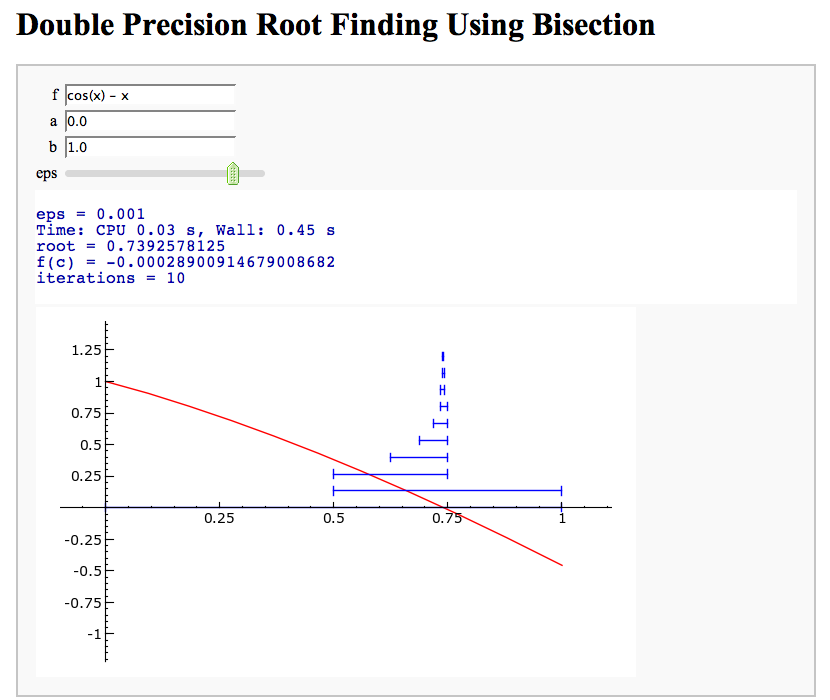
\includegraphics[width=8 cm,keepaspectratio=true]{bisection.png}

\end{center}
\index{fastapunktsaðferð}\index{fastapunktur}

\section{Fastapunktsaðferð}
\label{kafli02:fastapunktsafer}\label{kafli02:index-2}
Næsta aðferð sem við skoðum kallast fastapunktsaðferð (e. fixed point method) og
er til að finna fastapunkta en ekki núllstöðvar. Það er hins vegar hægt að
nota hana til þess að finna núllstöðvar, sjá athugasemd hér að {\hyperref[kafli02:fastapunktar-nullstodvar]{\emph{neðan}}}.


\subsection{Skilgreining}
\label{kafli02:id1}
Látum \(f : [a,b] \to \mathbb R\) vera samfellt fall. Punktur
\(r \in [a,b]\) þannig að
\begin{gather}
\begin{split}f(r) = r\end{split}\notag
\end{gather}
kallast \emph{fastapunktur} fallsins \(f\).

\begin{notice}{note}{Athugasemd:}
Athugum að í fastapunktum skerast graf fallsins \(y=f(x)\) og línan
\(y=x\). Verkefnið að ákvarða fastapunkta fallsins \(r\) er því
jafngilt því að athuga hvar graf \(f\) sker línuna \(y=x\).
\end{notice}


\subsection{Tenging við núllstöðvar}
\label{kafli02:fastapunktar-nullstodvar}\label{kafli02:tenging-vi-nullstovar}
Verkefnið að finna fastapunkta fallsins \(g(x)\) er jafngilt því að
finna núllstöðvar fallsins \(f(x)=g(x)-x\).

Þannig að ef við viljum t.d. finna núllstöð \(f(x) = e^x + x^3\) þá er nóg að finna fastapunkt
fallsins \(g(x) = e^x + x^3 + x\).


\subsection{Reiknirit}
\label{kafli02:reiknirit}
\textbf{Byrjunarskref:}      Valin er tala \(x_0\in [a,b]\).

\textbf{Ítrunarskref:}       Ef \(x_0,\dots,x_n\) hafa verið valin, þá setjum við
\begin{quote}
\begin{gather}
\begin{split}x_{n+1}=f(x_n)\end{split}\notag
\end{gather}\end{quote}

\begin{notice}{note}{Athugasemd:}
Til þess að þetta sé vel skilgreind runa, þá verðum við að gera ráð
fyrir að \(f(x)\in [a,b]\) fyrir öll \(x\in [a,b]\). Þetta
skilyrði er einnig skrifað
\begin{gather}
\begin{split}f([a,b])\subset [a,b].\end{split}\notag
\end{gather}\end{notice}

\begin{notice}{note}{Athugasemd:}
Ef \(f\) er samfellt og runan er samleitin með markgildið \(r\), þá er
\begin{gather}
\begin{split}r=\lim_{n\to \infty}x_{n+1}=\lim_{n\to \infty}f(x_{n})
=f(\lim_{n\to \infty}x_{n})=f(r).\end{split}\notag
\end{gather}
Þetta segir okkur að \emph{ef} við getum séð til þess að runan verði
samleitin, þá er markgildið fastapunktur.
\end{notice}

\index{herping}

\subsection{Skilgreining: Herping}
\label{kafli02:skilgreining-herping}\label{kafli02:index-3}
Fall \(f:[a,b]\to {\mathbb  R}\) er sagt vera \emph{herping} ef til er
fasti \(\lambda\in [0,1[\) þannig að
\begin{gather}
\begin{split}|f(x)-f(y)|\leq \lambda|x-y| \qquad \text{ fyrir öll } x,y\in [a,b].\end{split}\notag
\end{gather}
\begin{notice}{note}{Athugasemd:}
Sérhver herping er samfellt fall.
\end{notice}


\subsection{Setning}
\label{kafli02:setning}
Ef \(f\) er deildanlegt fall á \(]a,b[\), þá gefur
meðalgildissetningin okkur til er \(\xi\) milli \(x\) og
\(y\) þannig að
\begin{gather}
\begin{split}f(x)-f(y)=f'(\xi)(x-y).\end{split}\notag
\end{gather}
Ef til er \(\lambda\in[0,1[\) þannig að \(|f'(x)|\leq \lambda\)
fyrir öll \(x\in [a,b]\), þá er greinilegt að \(f\) er herping.

\index{fastapunktsaðferð!fastapunktssetningin}

\subsection{Fastapunktssetningin}
\label{kafli02:index-4}\label{kafli02:fastapunktssetningin}
Látum \(f : [a,b] \to [a,b]\) vera herpingu. Þá hefur \(f\)
nákvæmlega einn fastapunkt \(r\) á bilinu \([a,b]\) og runan
\((x_n)\) þar sem
\begin{gather}
\begin{split}\begin{aligned}
  x_0 &\in [a,b] \quad \text{ getur verið hvaða tala sem er  og } \\
  x_{n+1} &= f(x_n), \quad n \geq 0,\end{aligned}\end{split}\notag
\end{gather}
stefnir á fastapunktinn.

Sönnunina brjótum við upp í nokkur skref.

\textbf{1. skref, herping hefur í mesta lagi einn fastapunkt}

Sönnum þetta með mótsögn.

Gerum ráð fyrir að \(r\) og \(s\) séu tveir ólíkir fastapunktar
á \([a,b]\). Þá er
\begin{gather}
\begin{split}|r - s| = |f(r) - f(s)|
  \leq \lambda |r - s| < |r - s|\end{split}\notag
\end{gather}
því \(\lambda < 1\). Þetta fær ekki staðist, þannig að fjöldi
fastapunkta er í mesta lagi einn

\textbf{2. skref, fallið} \(f\) \textbf{hefur fastapunkt:}

Látum \(g(x) = f(x) - x\), þá eru núllstöðvar \(g\) nákvæmlega
fastapunktar \(f\).

Þar sem \(a \leq f(x) \leq b\) fyrir öll \(x \in [a,b]\) er
\begin{gather}
\begin{split}\left\{ \begin{array}{c}
      g(a) = f(a) - a \geq 0 \\
      g(b) = f(b) - b \leq 0
  \end{array} \right.\end{split}\notag
\end{gather}
Ef annað hvort \(g(a) = 0\) eða \(g(b) = 0\) höfum við fundið
fastapunkt fallsins \(f\) og við getum hætt.

Ef hins vegar \(g(a) > 0\) og \(g(b) < 0\) þá hefur \(g\)
ólík formerki í endapunktum bilsins \([a,b]\) og hefur því núllstöð
\(r\) á bilinu skv. milligildissetninguninni. Þá er \(r\)
jafnframt fastapunktur \(f\).

Skref 1 og 2 sýna því að fallið \(f\) hefur nákvæmlega einn
fastapunkt á bilinu.

\textbf{3. skref, runan} \((x_n)\) \textbf{er samleitin}

Látum \(r\) vera ótvírætt ákvarðaða fastapunktinn á \([a,b]\).

Við notfærum okkur að \(f\) er herping og að \(r\) er
fastapunktur \(f\), þá fæst að fyrir sérhvert
\(k\in {\mathbb  N}\) þá er
\begin{gather}
\begin{split}|r - x_k| = |f(r) - f(x_{k-1})|  \leq \lambda |r - x_{k-1}|\end{split}\notag
\end{gather}
það er \(|r - x_k| \leq \lambda |r - x_{k-1}|\).

Með því að nota þetta \(n\)-sinnum þá fæst að
\begin{gather}
\begin{split}\begin{aligned}
    |r - x_n|   &\leq \lambda |r - x_{n-1}| & (k=n)\\
    &\leq \lambda^2 |r - x_{n-2}| & (k=n-1)\\
    &\vdots & \vdots\\
    &\leq \lambda^n |r - x_0| & (k=1).
\end{aligned}\end{split}\notag
\end{gather}
Þar sem \(\lambda < 1\) er því
\begin{gather}
\begin{split}\lim\limits_{n \to +\infty} |r - x_n|
\leq \lim\limits_{n \to +\infty} \lambda^n |r - x_0|
= 0,\end{split}\notag
\end{gather}
það er runan \(x_n\) stefnir á \(r\).


\subsection{Fastapunktsaðferð er að minnsta kosti línulega samleitin}
\label{kafli02:fastapunktsafer-er-a-minnsta-kosti-linulega-samleitin}
Af skilgreiningunni á rununni \(x_n\) leiðir beint að
\begin{gather}
\begin{split}|e_{n+1}|=|r-x_{n+1}|=|f(r)-f(x_n)|\leq \lambda|r-x_n|=\lambda|e_n|\end{split}\notag
\end{gather}
sem segir okkur að fastapunktsaðferð sé að minnsta kosti línulega
samleitin ef \(f\) er herping.


\begin{center}
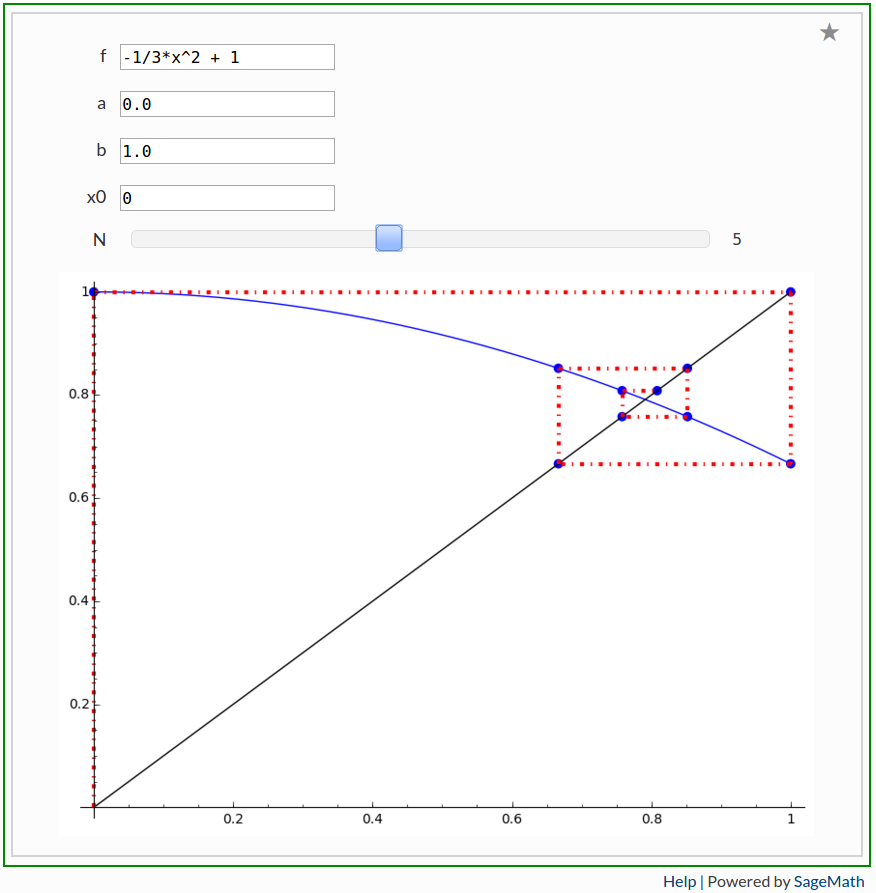
\includegraphics[width=8 cm,keepaspectratio=true]{fixedpoint.png}

\end{center}
\index{sniðilsaðferð}

\section{Sniðilsaðferð}
\label{kafli02:index-5}\label{kafli02:sniilsafer}
Næst er aðferð til að finna núllstöðvar sem kallast \emph{sniðilsaðferð}
(e. \href{https://en.wikipedia.org/wiki/Secant\_method}{secant method})

Gefið er fallið \(f:[a,b]\to {\mathbb  R}\). Við ætlum að ákvarða
núllstöð \(f\), þ.e.a.s. \(p\in [a,b]\) þannig að
\begin{gather}
\begin{split}f(p)=0.\end{split}\notag
\end{gather}
Rifjum upp að \emph{sniðill} við graf \(f\) gegnum punktana
\((\alpha,f(\alpha))\) og \((\beta,f(\beta))\) er gefinn með
jöfnunni
\begin{gather}
\begin{split}y=f(\alpha)+f[\alpha,\beta](x-\alpha)\end{split}\notag
\end{gather}
þar sem hallatalan er
\begin{gather}
\begin{split}f[\alpha,\beta]=\dfrac{f(\beta)-f(\alpha)}{\beta-\alpha}
=\dfrac{f(\alpha)-f(\beta)}{\alpha -\beta}.\end{split}\notag
\end{gather}
Sniðillinn sker \(x\)-ásinn í punkti \(s\) þar sem
\begin{gather}
\begin{split}0=f(\alpha)+f[\alpha,\beta](s-\alpha) \quad  \text{sem jafngildir því að } \quad
s=\alpha-\dfrac{f(\alpha)}{f[\alpha,\beta]}.\end{split}\notag
\end{gather}

\subsection{Reiknirit}
\label{kafli02:id2}
\textbf{Byrjunarskref:} Giskað er á tvö gildi \(x_0\) og \(x_1\).

\textbf{Ítrunarskref:} Fyrir \(n>1\) þá er punkturinn \(x_{n+1}\)
skilgreindur sem skurðpunktur sniðilsins gegnum \((x_{n-1},f(x_{n-1}))\) og
\((x_n,f(x_n))\) við \(x\)-ás, þ.e.
\begin{gather}
\begin{split}x_{n+1}=x_n-\dfrac{f(x_n)}{f[x_n,x_{n-1}]}.\end{split}\notag
\end{gather}

\subsection{Samleitin runa stefnir á núllstöð \(f\)}
\label{kafli02:samleitin-runa-stefnir-a-nullsto}
Gefum okkur að runan \((x_n)\) sé samleitin að markgildinu
\(r\). Meðalgildissetningin segir okkur þá að til sé punktur
\(\eta_n\) á milli \(x_{n-1}\) og \(x_n\) þannig að
\begin{gather}
\begin{split}f[x_n,x_{n-1}]=f'(\eta_n),\end{split}\notag
\end{gather}
og greinilegt er að \(\eta_n\to r\).

Við fáum því
\begin{gather}
\begin{split}r=\lim_{n\to \infty}x_{n+1}=\lim_{n\to \infty}
\bigg(x_n-\dfrac{f(x_n)}{f'(\eta_n)}\bigg) =r-\dfrac{f(r)}{f'(r)}\end{split}\notag
\end{gather}
Þessi jafna jafngildir því að \(f(r)=0\).


\subsection{Skekkjumat í nálgun á \(f(x)\) með \(p_n(x)\)}
\label{kafli02:skekkjumat-i-nalgun-a-me}
Sniðilinn sem við notum er graf 1. stigs margliðunnar
\begin{gather}
\begin{split}p_n(x) = f(x_n) +
        \dfrac{f(x_{n-1})-f(x_n)}{x_{n-1}-x_n}(x-x_n)
        = f(x_n) + f[x_n,x_{n-1}](x-x_n)\end{split}\notag
\end{gather}
Samkvæmt skilgreiningu er \(p_n(x_{n+1}) = 0\) svo \(x_{n+1}\)
uppfyllir jöfnuna
\begin{gather}
\begin{split}x_{n+1} = x_n - \frac{f(x_n)}{f[x_n,x_{n-1}]}.\end{split}\notag
\end{gather}
Við þurfum að vita hver skekkjan er á því að nálga \(f(x)\) með
\(p_n(x)\).

Niðurstaðan er að fyrir sérhvert \(x \in [a,b]\) er til
\(\xi_n\) sem liggur í minnsta bilinu sem inniheldur \(x\),
\(x_n\) og \(x_{n-1}\) þannig að
\begin{gather}
\begin{split}f(x) - p_n(x) = \frac{1}{2}f''(\xi_n)(x-x_n)(x-x_{n-1})\end{split}\notag
\end{gather}
Ljóst er að matið gildir ef \(x=x_{n-1}\) eða \(x=x_n\).

Festum því punktinn \(x\) og gerum ráð fyrir að \(x\neq x_1\) og
\(x\neq x_n\).

Skilgreinum fallið
\begin{gather}
\begin{split}g(t)=f(t)-p_n(t)-\lambda(t-x_n)(t-x_{n-1})\end{split}\notag
\end{gather}
þar sem \(\lambda\) er valið þannig að \(g(x)=0\).

Látum nú \(\alpha<\beta<\gamma\) vera uppröðun á punktunum
\(x_{n-1}\), \(x_n\) og \(x\).

Fallið
\begin{gather}
\begin{split}g(t)=f(t)-p_n(t)-\lambda(t-x_n)(t-x_{n-1})\end{split}\notag
\end{gather}
hefur núllstöð í öllum punktunum þremur.

Meðalgildissetningin gefur þá að \(g'(t)\) hefur eina núllstöð í
punkti á bilinu \(]\alpha,\beta[\) og aðra í \(]\beta,\gamma[\).

Af því leiðir aftur að \(g''(t)\) hefur núllstöð, \(\xi_n\), í
\([\alpha,\gamma]\), sem er minnsta bilið sem inniheldur alla
punktana \(x_{n-1}\), \(x_n\) og \(x\).

Af þessu leiðir
\begin{gather}
\begin{split}0=g''(\xi_n)=f''(\xi_n)-2\lambda \quad \text{þþaa} \quad
\lambda=\tfrac 12 f''(\xi_n).\end{split}\notag
\end{gather}
Nú var \(\lambda\) upprunalega valið þannig að \(g(x)=0\). Þar
með er
\begin{gather}
\begin{split}f(x) - p_n(x) = \frac{1}{2}f''(\xi_n)(x-x_n)(x-x_{n-1}).\end{split}\notag
\end{gather}

\subsection{Skekkjumat í sniðilsaðferð}
\label{kafli02:skekkjumat-i-sniilsafer}
Skoðum hvað af þessu leiðir:

Nú er \(f(r) = 0\) og því
\begin{gather}
\begin{split}-p_n(r) = \frac{1}{2}f''(\xi_n)e_n\cdot e_{n-1}.\end{split}\notag
\end{gather}
Eins er
\begin{gather}
\begin{split}-p_n(r) = -f[x_n,x_{n-1}]e_{n+1}=-f'(\eta_n)e_{n+1},\end{split}\notag
\end{gather}
þar sem \(\eta_n\) fæst úr meðalgildissetningunni og liggur á milli
\(x_n\) og \(x_{n+1}\). Niðurstaðan verður því
\begin{gather}
\begin{split}e_{n+1} = \frac{-\frac{1}{2}f''(\xi_n)}
        {f[x_n, x_{n+1}]}
    e_ne_{n-1} = \frac{-\frac{1}{2}f''(\xi_n)}
        {f'(\eta_n)}e_ne_{n-1}\end{split}\notag
\end{gather}
það er
\begin{gather}
\begin{split}\lim_{n\to \infty}\dfrac{e_{n+1}}{e_ne_{n-1}}=
\lim_{n \to \infty} \frac{-\frac{1}{2}f''(\xi_n)}
        {f'(\eta_n)}
=
\frac{-\frac{1}{2}f''(r)}
        {f'(r)}.\end{split}\notag
\end{gather}

\subsection{Setning}
\label{kafli02:id3}
Ef sniðilsaðferð er samleitin, \(f\in C^2([a,b])\) (tvisvar
diffranlegt) og \(f'(r)\neq 0\), þá er sniðilsaðferðin ofurlínuleg.
\begin{gather}
\begin{split}\lim_{n\to \infty}\dfrac{|e_{n+1}|}{|e_n|} =
\lim_{n\to \infty}\dfrac{|e_{n+1}e_{n-1}|}{|e_ne_{n-1}|}=
\lim_{n \to \infty} \frac{|e_{n-1}\frac{1}{2}f''(r)|}
        {|f'(r)|} = 0\end{split}\notag
\end{gather}
Raunar þá er sniðilsaðferðin samleitin af stigi
\(\alpha = (1+\sqrt 5)/2 \approx 1,618\) og með
\(\lambda = \left(\frac{f''(r)}{2f'(r)}\right)^{\alpha -1}\).

\index{aðferð Newtons}\index{snertill}

\section{Aðferð Newtons}
\label{kafli02:index-6}\label{kafli02:afer-newtons}
Í sniðilsaðferðinni létum við \(x_{n+1}\) vera skurðpunkt sniðils
gegnum \((x_{n-1},f(x_{n-1}))\) og \((x_n,f(x_n))\) við
\(x\)-ás og fengum við rakningarformúluna
\begin{gather}
\begin{split}x_{n+1} = x_n - \frac{f(x_n)}{f[x_n,x_{n-1}]}.\end{split}\notag
\end{gather}
Aðferð Newtons er nánast eins, nema í stað sniðils tökum við snertil í
punktinum \((x_n,f(x_n))\).

Rakningarformúlan er eins, nema hallatalan verður \(f'(x_n)\) í stað
\(f[x_n,x_{n-1}]\)


\subsection{Reiknirit}
\label{kafli02:id4}
\textbf{Byrjunarskref:} Giskað er á eitt gildi \(x_0\).

\textbf{Ítrunarskref:} Gefin eru \(x_0,\dots,x_n\). Punkturinn \(x_{n+1}\) er
skurðpunktur snertils gegnum \((x_n,f(x_n))\) við \(x\)-ás,
\begin{gather}
\begin{split}x_{n+1}=x_n-\dfrac{f(x_n)}{f'(x_n)}.\end{split}\notag
\end{gather}

\subsection{Upprifjun}
\label{kafli02:upprifjun}
Munum að snertill við graf \(f\) í punktinum \(x_n\) er
\begin{gather}
\begin{split}y=f(x_n) + f'(x_n)(x-x_n),\end{split}\notag
\end{gather}
þessi lína sker \(x\)-ásinn (\(y=0\)) þegar
\(x=x_n - \frac{f(x_n)}{f'(x_n)}\).


\subsection{Samleitin runa stefnir á núllstöð \(f\)}
\label{kafli02:id5}
Gefum okkur að runan \((x_n)\) sé samleitin með markgildið
\(r\). Við fáum því
\begin{gather}
\begin{split}r=\lim_{n\to \infty}x_{n+1}=\lim_{n\to \infty}
\bigg(x_n-\dfrac{f(x_n)}{f'(x_n)}\bigg) =r-\dfrac{f(r)}{f'(r)}\end{split}\notag
\end{gather}
Þessi jafna jafngildir því að \(f(r)=0\).

Þannig að ef runan er samleitin þá fáum við núllstöð.


\subsection{Skekkjumat í nálgun á \(f(x)\) með \(p_n(x)\)}
\label{kafli02:id6}
Snertillinn við \(f\) í punktinum \(x_n\) er 1. stigs margliðan
\begin{gather}
\begin{split}p_n(x) = f(x_n) + f'(x_n)(x-x_n)\end{split}\notag
\end{gather}
Samkvæmt skilgreiningu er \(p_n(x_{n+1}) = 0\) svo \(x_{n+1}\)
uppfyllir jöfnuna
\begin{gather}
\begin{split}x_{n+1} = x_n - \frac{f(x_n)}{f'(x_n)}.\end{split}\notag
\end{gather}
Athugum að \(p_n\) er fyrsta Taylor nálgunin við fallið \(f\)
kringum \(x_n\). Setning Taylors gefur að til er \(\xi_n\) sem
liggur á milli \(r\) og \(x_n\) þannig að
\begin{gather}
\begin{split}f(r) - p_n(r) = \frac{1}{2}f''(\xi_n)(r-x_n)^2.\end{split}\notag
\end{gather}

\subsection{Skekkjumat í aðferð Newtons}
\label{kafli02:skekkjumat-i-afer-newtons}
Nú er \(f(r) = 0\) og því
\begin{gather}
\begin{split}-p_n(r) = \frac{1}{2}f''(\xi_n)e_n^2.\end{split}\notag
\end{gather}
Eins er fæst af skilgreiningunni á \(p_n\) að
\begin{gather}
\begin{split}-p_n(r) = -f'(x_n)e_{n+1}\end{split}\notag
\end{gather}
Niðurstaðan verður því
\begin{gather}
\begin{split}e_{n+1} = \frac{-\frac{1}{2}f''(\xi_n)}
        {f'(x_n)}e_n^2\end{split}\notag
\end{gather}

\begin{center}
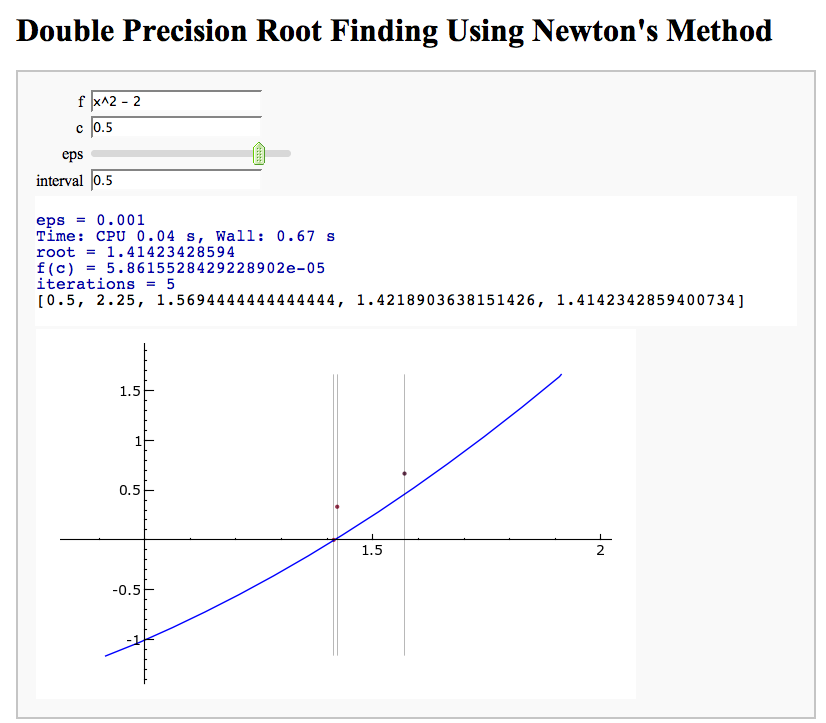
\includegraphics[width=8 cm,keepaspectratio=true]{newton.png}

\end{center}

\subsection{Setning}
\label{kafli02:id7}
Ef aðferð Newtons fyrir fallið \(f\) er samleitin,
\(f\in C^2([a,b])\) og \(f'(r)\neq 0\), þá fáum við:
\begin{gather}
\begin{split}\lim_{n\to \infty}\dfrac{e_{n+1}}{e_n^2}=\frac{-\frac{1}{2}f''(r)}
        {f'(r)}\end{split}\notag
\end{gather}
Það þýðir að aðferð Newtons er ferningssamleitin.
\begin{gather}
\begin{split}\lim_{n\to \infty}\dfrac{e_{n+1}}{e_n^2}=
\lim_{n\to \infty}\frac{-\frac{1}{2}f''(\xi_n)}{f'(x_n)} =
\frac{-\frac{1}{2}f''(r)}{f'(r)}\end{split}\notag
\end{gather}
\begin{notice}{note}{Athugasemd:}
Athugið að það er ekki sjálfgefið að aðferð Newtons sé samleitin.

Auðvelt er að finna dæmi þar sem vond upphafságiskun \(x_0\) skilar
runu sem er ekki samleitin.
\end{notice}


\section{Samanburður á aðferðum}
\label{kafli02:samanburur-a-aferum}
\begin{tabular}{|l|l|l|}
\hline
\textsf{\relax 
Aðferð
} & \textsf{\relax 
Samleitni
} & \textsf{\relax 
Stig samleitni
}\\


\hline 
{\hyperref[kafli02:helmingunarafer]{\emph{Helmingunaraðferð}}}
(e. \href{https://en.wikipedia.org/wiki/Bisection\_method}{bisection method})
 &  Já, ef \(f(a)f(b)<0\) & 1, línuleg\\\hline
 \hyperref[kafli02:fastapunktsafer]{\emph{Fastapunktsaðferð}}
(e. \href{https://en.wikipedia.org/wiki/Fixed-point\_iteration}{fixed point iteration})
 & Ekki alltaf. En saml. ef \(f\) er herping  &  amk 1
\\\hline
\hyperref[kafli02:sniilsafer]{\emph{Sniðilsaðferð}}
(e. \href{https://en.wikipedia.org/wiki/Secant\_method}{secant method})
 &  Ekki alltaf & \(\approx 1,618\), ef \(f'(r)\neq 0\)
\\\hline
{\hyperref[kafli02:afer-newtons]{\emph{Aðferð Newtons}}}
(e. \href{https://en.wikipedia.org/wiki/Newton\%27s\_method}{Newtons method})
 & Ekki alltaf & 2, ef \(f'(r)\neq 0\)\\
 \end{tabular}

\begin{notice}{warning}{Aðvörun:}
Þó að aðferð Newtons sé samleitin af stigi 2, en sniðilsaðferðin af
stigi u.þ.b. 1,618, þá er í vissum tilfellum hagkvæmara að nota
sniðilsaðferðina ef það er erfitt að reikna gildin á afleiðunni
\(f'\).
\end{notice}


\chapter{Brúun}
\label{kafli03::doc}\label{kafli03:bruun}
\emph{Over the centuries, mankind has tried many ways of combating the forces of evil...
prayer, fasting, good works and so on. Up until Doom, no one seemed to have thought
about the double-barrel shotgun. Eat leaden death, demon.}
-- Terry Pratchett


\section{Inngangur}
\label{kafli03:inngangur}
\index{brúun}\index{brúunarmargliða}\index{brúunarpunktur}

\subsection{Markmiðið}
\label{kafli03:index-0}\label{kafli03:markmii}
Viðfangsefni þessa kafla er að finna ferla sem ganga gegnum fyrirfram
gefna \emph{brúunarpunkta} \((x_0,y_0),\dots,(x_m,y_m)\) í planinu eða liggja nálægt
punktunum í einhverjum skilningi.

Fyrst viljum við finna graf margliðu \(p\) sem fer gegnum punktana.
Þá þurfum við að gefa okkur að \(x_i\neq x_j\) ef \(i\neq j\).

Við sýnum fram á að það sé alltaf hægt að finna margliðu \(p\) af
stigi \(\leq m\) sem uppfyllir \(p(x_i)=y_i\) í öllum punktum og
að slík margliða sé ótvírætt ákvörðuð.

Hún nefnist \emph{brúunarmargliða} fyrir punktana
\((x_0,y_0),\dots,(x_m,y_m)\).

Við alhæfum þetta verkefni með því að úthluta sérhverjum punkti jákvæðri
heiltölu \(m_i\) og krefjast þess graf margliðunnar fari í gegnum
alla punktana og til viðbótar að allar afleiður \(p^{(j)}\) upp að
stigi \(m_i-1\) taki einnig fyrirfram gefin gildi \(y^{(j)}_i\).


\subsection{Brúun}
\label{kafli03:id1}
Við tilraunir þá fáum við oft aðeins strjálar mælingar, t.d. ef við
mælum hljóðhraða við mismunandi hitastig. Hins vegar þá viljum við vita
hvert sambandið er fyrir öll möguleg hitastig. Brúunin er margliða og
hún skilgreind er fyrir allar rauntölur og {}`{}`brúar{}`{}` því gildin
milli mælipunktanna.

\index{setning Weierstrass}

\subsection{Afhverju margliður?}
\label{kafli03:index-1}\label{kafli03:afhverju-margliur}\begin{itemize}
\item {} 
Einfalt að meta fallgildin fyrir margliður ({\hyperref[kafli03:reiknirit-horners]{Reiknirit Horners}}).

\item {} 
Einfalt að diffra og heilda margliður.

\item {} 
Margliður eru óendanlega oft diffranlegar.

\item {} 
\emph{Setning Weierstrass:} Látum \(f\) vera samfellt fall á bili
\([a,b]\). Fyrir sérhvert \({\varepsilon}> 0\) þá er til
margliða \(p\) þannig að
\begin{gather}
\begin{split}\|f-p\|_\infty := \max_{x\in [a,b]} |f(x)-p(x)| < {\varepsilon}.\end{split}\notag
\end{gather}
\end{itemize}

\begin{notice}{note}{Athugasemd:}
Setning Weierstrass segir að margliður nægja til að nálga samfelld föll.
Það er sama hvað samfellda fall við skoðum það er alltaf til margliða
sem nálgar það eins vel og við viljum á lokuðu bili.
\end{notice}

\index{margliður}\index{margliður!stig}

\subsection{Margliður}
\label{kafli03:index-2}\label{kafli03:margliur}
Fall \(p\) af gerðinni
\begin{gather}
\begin{split}p(x) = a_0 + a_1 x + \ldots + a_m x^m\end{split}\notag
\end{gather}
þar sem \(m\) er heiltala og \(a_0, \ldots, a_m\) eru tvinntölur
nefnist margliða.

Stærsta talan \(j\) þannig að \(a_j \not= 0\) nefnist \emph{stig
margliðunnar} \(p\).

Ef allir stuðlarnir eru 0 þá nefnist \(p\) \emph{núllmargliðan} og við
segjum að stig hennar sé \(-\infty\).

Munum að stuðullinn \(a_j\) við veldið \(x^j\) er gefinn með
formúlunni
\begin{gather}
\begin{split}a_j = \frac{p^{(j)}(0)}{j!}, \quad j = 0,1,2,\ldots,m.\end{split}\notag
\end{gather}
\index{margliður!staðalform}

\subsection{Mismunandi leiðir á framsetningu}
\label{kafli03:mismunandi-leiir-a-framsetningu}\label{kafli03:index-3}
Hægt er að setja sömu margliðuna fram á marga mismunandi vegu, en við
nefnum framsetninguna hér að framan \emph{staðalform margliðunnar} \(p\).

Ef við veljum okkur einhvern punkt \(x_0 \in {{\mathbb  R}}\), þá
getum við skrifað
\begin{gather}
\begin{split}p(x) = b_0 + b_1(x-x_0) + \ldots + b_m(x-x_0)^m\end{split}\notag
\end{gather}
og stuðlarnir \(b_j\) eru gefnir með
\begin{gather}
\begin{split}b_j = \frac{p^{(j)}(x_0)}{j!}, \quad j = 0,1,2,\ldots,m.\end{split}\notag
\end{gather}
Þessi formúla er jafngild þeirri staðreynd að ef \(p\) er margliða
af stigi \(m\). Þá er Taylor-röð \(p\) í sérhverjum punkti
\(x_0 \in {{\mathbb  R}}\) bara margliðan \(p\), og stuðlarnir í
Taylor-röðinni eru gefnir með formúlunum fyrir \(b_j\) að ofan.

\index{margliður!Newton-form}

\subsection{Newton-form margliðu}
\label{kafli03:index-4}\label{kafli03:newton-form-margliu}
Ef við veljum okkur \(m\) punkta \(x_0, \ldots, x_{m-1}\) þá
nefnist framsetning af gerðinni
\begin{gather}
\begin{split}p(x) = c_0 + c_1(x-x_0) + c_2(x-x_0)(x-x_1)
    + \ldots + c_m(x-x_0)\cdots(x-x_{m-1})\end{split}\notag
\end{gather}
\emph{Newton-form} margliðunnar \(p\) miðað við punktana
\(x_0, \ldots,
x_{m-1}\).

\index{reiknirit Horners}

\subsection{Reiknirit Horners}
\label{kafli03:index-5}\label{kafli03:reiknirit-horners}
Við munum mikið fást við margliður á Newton-formi og því er nauðsynlegt
að hafa hraðvirkt reiknirit til þess að reikna út fallgildi \(p\) út
frá þessari framsetningu.

Eitt slíkt reiknirit er nefnt \emph{reiknirit Horners}. Það byggir á því að
nýta sér að þættirnir \((x-x_j)\) eru endurteknir í liðunum
\begin{gather}
\begin{split}(x-x_0), \quad (x-x_0)(x-x_1),
    \quad (x-x_0)(x-x_1)(x-x_2), \quad \ldots\end{split}\notag
\end{gather}
Þar sem við sleppum við að hefja í veldi þá komumst við af með fáar
reikniaðgerðir hér.

Ef \(m = 2\) má skrifa Newton-form \(p\) sem
\begin{gather}
\begin{split}p(x) = c_0 + (x-x_0)(c_1 + (x-x_1) \cdot c_2).\end{split}\notag
\end{gather}
Ef \(m = 3\) er það
\begin{gather}
\begin{split}p(x) = c_0 + (x-x_0)(c_1 + (x-x_1)(c_2 + (x-x_2)c_3))\end{split}\notag
\end{gather}
og ef \(m = 4\) er það
\begin{gather}
\begin{split}p(x) = c_0 + (x-x_0)(c_1 + (x-x_1)(c_2 + (x-x_2)
    (c_3 + c_4(x-x_3)))).\end{split}\notag
\end{gather}
Reikniritið vinnur á þessari stæðu með því að margfalda upp úr svigunum
frá hægri til vinstri.

Skilgreinum tölur \(b_0\), \(b_1\), \(\ldots\) á
eftirfarandi hátt. Fyrst setjum við
\begin{gather}
\begin{split}b_n = c_n.\end{split}\notag
\end{gather}
Fyrir hvert \(k\) frá \(n-1\) niður í 0 þá setjum við
\begin{gather}
\begin{split}b_k = c_k + (a - x_k) b_{k+1}.\end{split}\notag
\end{gather}
Þá er \(b_0 = p(a)\).
\begin{gather}
\begin{split}p(a) =
    \underbrace{
      c_0 + (a-x_0)(
      \underbrace{
        c_1 + (a-x_1)(
          \underbrace{c_2 + (a-x_2)(
        \underbrace{c_3 + (a-x_3)
          \underbrace{c_4}_{b_4}
          }_{b_3})
        }_{b_2})
      }_{b_1})
    }_{b_0}.\end{split}\notag
\end{gather}
\index{brúun!brúunarmargliða}\index{brúun!brúunarverkefni}

\section{Margliðubrúun: Lagrange-form}
\label{kafli03:margliubruun-lagrange-form}\label{kafli03:index-6}

\subsection{Margliðubrúun}
\label{kafli03:margliubruun}
Látum nú \((x_0,y_0), \ldots, (x_m,y_m)\) vera gefna punkta í plani.
Við höfum áhuga á að finna margliðu \(p\) af lægsta mögulega stigi
þannig að
\begin{gather}
\begin{split}p(x_k) = y_k, \quad k = 0, \ldots, m.\end{split}\notag
\end{gather}
Slík margliða nefnist \emph{brúunarmargliða} fyrir punktana
\((x_0,y_0), \ldots, (x_m,y_m)\)

eða \emph{brúunarmargliða gegnum punktana}
\((x_0,y_0), \ldots, (x_m,y_m)\).

Augljóslega verðum við að gera ráð fyrir að \(x\)-hnitin séu ólík,
það er \(x_j \not= x_k\) ef \(j \not= k\).

Verkefnið að finna margliðuna \(p\) nefnist \emph{brúunarverkefni fyrir
punktana} \((x_0,y_0), \ldots, (x_m,y_m)\).


\subsection{Setning: Brúunarmargliðan er ótvírætt ákvörðuð}
\label{kafli03:setning-bruunarmarglian-er-otviraett-akvoru}
Brúunarmargliðan af stigi \(\leq m\) fyrir \((x_0,y_0),\ldots,(x_m,y_m)\) er
ótvírætt ákvörðuð.

Ef \(p(x)\) og \(q(x)\) eru tvær
brúunarmargliður af stigi \(\leq m\) fyrir punktana
\((x_0,y_0), \ldots, (x_m,y_m)\) þá er mismunurinn
\(r(x) = p(x) - q(x)\) margliða af stigi \(\leq m\) með
núllstöðvar \(x_0, \ldots, x_m\). Þetta eru \(m+1\) ólíkir
punktar og því er \(r(x)\) núllmargliðan samkvæmt
\href{http://www.stae.is/fletta/undirst\%C3\%B6\%C3\%B0usetning/algebrunnar}{undirstöðusetningu algebrunnar}.
Þar með er \(p(x) - q(x)\) núllmargliðan, þ.e. \(p(x) = q(x)\).


\subsection{Setning: Brúunarmargliðan er til}
\label{kafli03:setning-bruunarmarglian-er-til}
Til er margliða \(p\) af stigi \(\leq m\) þannig að
\begin{gather}
\begin{split}p(x_0) = y_0, \quad \ldots \quad p(x_n)=y_n.\end{split}\notag
\end{gather}
Við notum þrepun til að sýna fram á tilvistina.

Ef \(m = 0\), þá erum við aðeins með eitt brúunarskilyrði,
\(p(x_0) = y_0\), og fastamargliðan \(p(x) = y_0\) er lausn af
stigi \(\leq 0\).

G.r.f. að við getum leyst öll brúunarverkefni þar sem fjöldi punkta er
\(m\) og sýnum að við getum þá leyst verkefnið fyrir \(m+1\)
punkt.

Látum \(q\) vera brúunarmargliðuna af stigi \(\leq m-1\) fyrir
punktana \((x_0,y_0), \ldots,
(x_{m-1},y_{m-1})\) og \(r\) vera brúunarmargliðuna af stigi
\(\leq m-1\) fyrir punktana \((x_1,y_1), \ldots, (x_m,y_m)\) og
setjum síðan
\begin{gather}
\begin{split}p(x) = \frac{x-x_m}{x_0-x_m}q(x) + \frac{x-x_0}{x_m-x_0}r(x),\end{split}\notag
\end{gather}
\(p(x)\) er greinilega margliða af stigi \(\leq m\). Skoðum nú
gildin á \(p\)
\begin{gather}
\begin{split}\begin{aligned}
  p(x_0) &= 1 \cdot q(x_0) + 0\cdot r(x_0) = y_0, \\
  p(x_k) &= \frac{x_k-x_m}{x_0-x_m}y_k
  + \frac{x_k-x_0}{x_m-x_0}y_k = y_k,\qquad k = 1, \ldots, m-1,\\
  p(x_m) &= 0 \cdot q(x_m) + 1 \cdot r(x_m) = y_m.\end{aligned}\end{split}\notag
\end{gather}
Þar með er \(p\) brúunarmargliðan sem uppfyllir \(p(x_j)=y_j\)
fyrir \(j=0,\dots,m\) og við höfum leyst brúunarverkefnið fyrir
\(m+1\) punkt.

\index{margliður!Lagrange-form}

\subsection{Lagrange-form brúunarmargliðunnar}
\label{kafli03:index-7}\label{kafli03:lagrange-form-bruunarmargliunnar}
Sönnunin á undan er í raun rakningarformúla til þess að reikna út gildi
brúunarmargliðunnar \(p\) fyrir punktana
\((x_0,y_0),\dots,(x_m,y_m)\).

Hægt er að skrifa lausnina niður beint
\begin{gather}
\begin{split}p(x)=y_0\ell_0(x)+y_1\ell_1(x)+\cdots+y_m\ell_m(x),\end{split}\notag
\end{gather}
þar sem \(\ell_0,\dots,\ell_m\) er ákveðinn grunnur fyrir rúm allra
margliða \({\cal P}_m\) af stigi \(\leq m\) og nefnast
\emph{Lagrange-margliður fyrir punktasafnið}
\((x_0,y_0),\dots,(x_m,y_m)\).


\subsection{Lagrange-margliður, tilfellin \(m=0,1,2\)}
\label{kafli03:lagrange-margliur-tilfellin}\begin{itemize}
\item {} 
\(m=0\) Ef \(m = 0\) þá er \(p(x) = y_0\) fastamargliða
eins og við höfum séð.

\item {} 
\(m=1\) Ef \(m = 1\), þá blasir við að lausnin er
\begin{gather}
\begin{split}p(x) = y_0 \frac{(x-x_1)}{(x_0-x_1)}
  + y_1 \frac{(x-x_0)}{(x_1-x_0)},\end{split}\notag
\end{gather}
sem er margliða af stigi \(\leq 1\) (þ.e. lína) sem leysir
brúunarverkefnið.

\item {} 
\(m=2\) Á hliðstæðan hátt fáum við fyrir \(m = 2\) að
\begin{gather}
\begin{split}p(x) = y_0 \frac{(x-x_1)(x-x_2)}{(x_0-x_1)(x_0-x_2)}
  + y_1 \frac{(x-x_0)(x-x_2)}{(x_1-x_0)(x_1-x_2)}
  + y_2 \frac{(x-x_0)(x-x_1)}{(x_2-x_0)(x_2-x_1)}\end{split}\notag
\end{gather}
leysir brúunarverkefnið.

\end{itemize}


\subsection{Lagrange-margliður almenna tilfellið}
\label{kafli03:lagrange-margliur-almenna-tilfelli}
Almennt fæst lausnin
\begin{gather}
\begin{split}\label{p}
  p(x) = y_0 \, \ell_{0}(x) + y_1 \, \ell_{1}(x)
  + \ldots + y_m \, \ell_{m}(x)\end{split}\notag
\end{gather}
þar sem
\begin{gather}
\begin{split}\ell_{k} = \prod\limits_{\stackrel{j=0}{j\not=k}}^m
  \frac{(x-x_j)}{(x_k-x_j)}\end{split}\notag
\end{gather}
\begin{notice}{note}{Athugasemd:}\begin{gather}
\begin{split}\label{l}
  \ell_{k}(x_i) = \left\{ \begin{array}{cc}
      1 & \text{ef } i = k \\
      0 & \text{ef } i \not= k
  \end{array} \right.\end{split}\notag
\end{gather}\end{notice}

Allar margliðurnar \(\ell_{k}\) eru af stigi \(m\) og því er
\(p\) af stigi \(\leq m\). Nú er augljóst útfrá ({[}p{]}) og ({[}l{]})
að \(p\) er lausn brúunarverkefnisins.


\subsection{Sýnidæmi}
\label{kafli03:synidaemi}
Finnið brúunarmargliðuna gegnum punktana \((1,1)\), \((2,3)\)
og \((3,6)\) með því að nota Lagrange-margliður.

Reiknum fyrst margliðurnar \(\ell_{0}\), \(\ell_{1}\) og
\(\ell_{2}\):
\begin{gather}
\begin{split}\begin{aligned}
  \ell_{0} &= \frac{(x-2)(x-3)}{(1-2)(1-3)}
  = \frac{(x-2)(x-3)}{2} \\
  \ell_{1} &= \frac{(x-1)(x-3)}{(2-1)(2-3)}
  = -(x-1)(x-3) \\
  \ell_{2} &= \frac{(x-1)(x-2)}{(3-1)(3-2)}
  = \frac{(x-1)(x-2)}{2}\end{aligned}\end{split}\notag
\end{gather}
Þá fæst að brúunarmargliðan \(p\) er
\begin{gather}
\begin{split}p(x) = 1 \cdot \frac{(x-2)(x-3)}{2}
  - 3 \cdot (x-1)(x-3)
  + 6 \cdot \frac{(x-1)(x-2)}{2}\end{split}\notag
\end{gather}
Þetta er greinilega annars stigs margliða og auðvelt er að sannfæra sig
um að \(p(1) = 1\), \(p(2) = 3\) og \(p(3) = 6\).

\index{brúun!Newton-form}

\section{Margliðubrúun: Newton-form}
\label{kafli03:index-8}\label{kafli03:margliubruun-newton-form}

\subsection{Formúla fyrir \(c_0, \ldots, c_m\)}
\label{kafli03:formula-fyrir}
Nú ætlum við að leiða út formúlu fyrir stuðlunum
\(c_0, \ldots, c_m\) í Newton-formi brúunarmargliðunnar \(p\)
miðað við röð brúunarpunktanna \(x_0, \ldots, x_{m-1}\).

Athugum að \(c_m = a_m\), þar sem \(a_m\) er stuðullinn við
veldið \(x^m\) í staðalframsetningunni á \(p\).

Til þess að reikna út \(c_0, \ldots, c_m\) þurfum við að reikna út
með skipulegum hætti stuðulinn við veldið \(x^j\) í
brúunarmargliðunni gegnum punktana
\((x_i,y_i), \ldots, (x_{i+j},y_{i+j})\), fyrir öll
\(i = 0, \ldots, m\) og \(j = 0, \ldots, m-i\). Við táknum
þennan stuðul með \(y[x_i, \ldots, x_{i+j}]\).

\begin{notice}{warning}{Aðvörun:}
Verkefnið er háð röð punktanna, þ.e. framsetningin (Newton-formið) á
margliðunni breytist eftir röð punktanna.
En auðvitað er margliðan og gildin á henni alltaf þau sömu

\emph{Dæmi:} Skoðum margliðuna \(p(x) = 2-7x+5x^2\).

Ef \(x_0=0\) og \(x_1=2\) þá er Newton-form hennar
\begin{gather}
\begin{split}p(x) = 3 + 3(x-0) + 5(x-0)(x-2).\end{split}\notag
\end{gather}
En ef \(x_0=2\) og \(x_1=0\) þá er Newton-form hennar
\begin{gather}
\begin{split}p(x) = 8 + 3(x-2) + 5(x-2)(x-0).\end{split}\notag
\end{gather}\end{notice}

\index{mismunakvóti}

\subsection{Mismunakvótar}
\label{kafli03:mismunakvotar}\label{kafli03:index-9}
Skilgreinum mismunakvóta \(y[x_i,\ldots,x_{i+j}]\) fyrir
punktasafnið \((x_i,y_i),\ldots,(x_{i+j},y_{i+j})\) á eftirfarandi
hátt:
\begin{itemize}
\item {} 
\(j=0\): \(y[x_i] = y_i\).

\item {} 
\(j=1\): \(y[x_i,x_{i+1}] = \frac{y_{i+1}-y_i}{x_{i+1}-x_i}\)

\item {} 
\(j=2\):
\(y[x_i,x_{i+1},x_{i+2}] = \frac{y[x_{i+1},x_{i+2}] - y[x_i,x_{i+1}]}{x_{i+2}-x_i}\).

\item {} 
\(j>2\):
\(y[x_i,\ldots,x_{i+j}] = \frac{y[x_{i+1},\ldots,x_{i+j}] - y[x_i,\ldots,x_{i+j-1}]}{x_{i+j}-x_i}\).

\end{itemize}

\begin{notice}{note}{Athugasemd:}
Stærðin \(y[x_{n-1},x_n]\) hefur komið fyrir áður
hjá okkur þegar við fjölluðum um \emph{Sniðilsaðferð}, enda er sniðill
ekkert annað en brúunarmargliða fyrir tvö punkta í planinu.
\end{notice}


\subsection{Upprifjun á tilvistarsönnuninni}
\label{kafli03:upprifjun-a-tilvistarsonnuninni}
Þrepunarskrefið í tilvistarsönnuninni
fyrir brúunarmargliður gefur okkur nú hvernig mismunakvótarnir nýtast okkur.

Látum \(q\) vera brúunarmargliðuna af stigi \(\leq m-1\) fyrir
punktana \((x_0,y_0), \ldots,
(x_{m-1},y_{m-1})\) og \(r\) vera brúunarmargliðuna af stigi
\(\leq m-1\) fyrir punktana \((x_1,y_1), \ldots, (x_m,y_m)\) og
setjum síðan
\begin{gather}
\begin{split}p(x) = \frac{x-x_m}{x_0-x_m}q(x) + \frac{x-x_0}{x_m-x_0}r(x)\end{split}\notag
\end{gather}
Gerum nú ráð fyrir að stuðullinn við veldið \(x^{m-1}\) í
\(q(x)\) sé \(y[x_0, \ldots, x_{m-1}]\) og stuðullinn við veldið
\(x^{m-1}\) í \(r(x)\) sé \(y[x_1, \ldots, x_m]\).

Við sjáum þá að stuðullinn við veldið \(x^m\) í \(p(x)\) er
\begin{gather}
\begin{split}\frac{y[x_0, \ldots, x_{m-1}]}{x_0-x_m} +
  \frac{y[x_1, \ldots, x_m]}{x_m - x_0}
  = y[x_0, \ldots, x_m]\end{split}\notag
\end{gather}
\begin{notice}{note}{Athugasemd:}
Fyrir \(m=0\) gildir að \(p(x) = y_0 = y[x_0]\).
\end{notice}

\index{brúun!mismunakvótatafla}

\subsection{Mismunakvótatöflur fyrir \(m=0,1,2,3\)}
\label{kafli03:index-10}\label{kafli03:mismunakvotatoflur-fyrir}
Mismunakvótar eru venjulega reiknaðir út í svokölluðum
\emph{mismunakvótatöflum}.

Ef \(m = 0\) er mismunakvótataflan aðeins ein lína
\begin{gather}
\begin{split}\begin{array}{c|c|c}
    i & x_i & y[x_i] \\
    \hline
    0 & x_0 & y[x_0] = y_0
  \end{array}\end{split}\notag
\end{gather}
Ef \(m = 1\) er taflan
\begin{gather}
\begin{split}\begin{array}{c|c|cc}
    i & x_i & y[x_i] & y[x_i,x_{i+1}] \\
    \hline
    0 & x_0 & y[x_0] = y_0 & y[x_0,x_1] \\
    1 & x_1 & y[x_1] = y_1 &
  \end{array}\end{split}\notag
\end{gather}
og margliðan er
\begin{gather}
\begin{split}p(x) = y[x_0] + y[x_0,x_1](x-x_0).\end{split}\notag
\end{gather}
Ef \(m = 2\) verður taflan
\begin{gather}
\begin{split}\begin{array}{c|c|ccc}
    i & x_i & y[x_i] & y[x_i,x_{i+1}] & y[x_i,x_{i+1},x_{i+2}] \\
    \hline
    0 & x_0 & y[x_0] = y_0 & y[x_0,x_1] & y[x_0,x_1,x_2] \\
    1 & x_1 & y[x_1] = y_1 & y[x_1,x_2] & \\
    2 & x_2 & y[x_2] = y_2 &  &
  \end{array}\end{split}\notag
\end{gather}
og margliðan er
\begin{gather}
\begin{split}p(x) = y[x_0] + y[x_0,x_1](x-x_0)
  + y[x_0,x_1,x_2](x-x_0)(x-x_1).\end{split}\notag
\end{gather}
Skoðum loks tilfellið \(m = 3\)
\begin{gather}
\begin{split}\begin{array}{c|c|cccc}
    i & x_i & y[x_i] & y[x_i,x_{i+1}] & y[x_i,x_{i+1},x_{i+2}]
    & y[x_i,x_{i+1},x_{i+2},x_{i+3}] \\
    \hline
    0 & x_0 & y[x_0] = y_0 & y[x_0,x_1] & y[x_0,x_1,x_2]
    & y[x_0,x_1,x_2,x_3] \\
    1 & x_1 & y[x_1] = y_1 & y[x_1,x_2] & y[x_1,x_2,x_3] & \\
    2 & x_2 & y[x_2] = y_2 & y[x_2,x_3] & & \\
    3 & x_3 & y[x_3] = y_3 & & &
  \end{array}\end{split}\notag
\end{gather}
Brúunarmargliðan fæst svo með því að nota stuðlana úr fyrstu línu
töflunnar:
\begin{gather}
\begin{split}\begin{aligned}
  p(x) = &y[x_0] + y[x_0,x_1](x-x_0)
  + y[x_0,x_1,x_2](x-x_0)(x-x_1) \\
  &+ y[x_0,x_1,x_2,x_3](x-x_0)(x-x_1)(x-x_2)\end{aligned}\end{split}\notag
\end{gather}

\subsection{Sýnidæmi}
\label{kafli03:id2}
Við skulum reikna út aftur brúunarmargliðuna gegnum \((1,1)\),
\((2,3)\) og \((3,6)\).

Stillum fyrst upp mismunakvótatöflu
\begin{gather}
\begin{split}\begin{array}{cc||ccc}
    i & x_i & y[x_i] & y[x_i,x_{i+1}] & y[x_i,x_{i+1},x_{i+2}] \\
    \hline
    0 & 1   &  1     &    &   \\
    1 & 2   &  3     &    &   \\
    2 & 3   &  6     &    &
  \end{array}\end{split}\notag
\end{gather}
Fyllum svo út í hana með að ganga á hvern dálk á fætur öðrum
\begin{gather}
\begin{split}\begin{array}{cc||ccc}
    i & x_i & y[x_i] & y[x_i,x_{i+1}] & y[x_i,x_{i+1},x_{i+2}] \\
    \hline
    0 & 1 & 1 & \dfrac{3-1}{2-1} = 2 & \dfrac{3-2}{3-1} = 1/2  \\
    1 & 2 & 3 & \dfrac{6-3}{3-2} = 3 & \\
    2 & 3 & 6 & &
  \end{array}\end{split}\notag
\end{gather}
Lesum út brúunarmargliðuna \(p\) með að ganga á efstu línuna:
\begin{gather}
\begin{split}p(x) = 1 + 2 \cdot (x-1) + \frac{1}{2} \cdot (x-1)(x-2).\end{split}\notag
\end{gather}
Reiknum út brúunarmargliðuna gegnum \((3,1)\), \((1,-3)\),
\((5,2)\) og \((6,4)\). Stillum upp og fyllum út í
mismunakvótatöflu:
\begin{gather}
\begin{split}\begin{array}{cc||cccc}
    i & x_i & y[x_i], & y[x_i,x_{i+1}], &
    y[x_i,x_{i+1},x_{i+2}], & y[x_i,\ldots,x_{i+3}] \\
    \hline
    1 & 3 & 1 & \frac{-3-1}{1-3} = 2 & \frac{5/4-2}{5-3} = -3/8 &
    \frac{3/20-(-3/8)}{6-3} = 7/40 \\
    2 & 1 & -3 & \frac{2-(-3)}{5-1} = 5/4 &
    \frac{2-5/4}{6-1} = 3/20 & \\
    3 & 5 & 2 & \frac{4-2}{6-5} = 2 & & \\
    4 & 6 & 4 & & &
  \end{array}\end{split}\notag
\end{gather}
Nú getum við lesið brúunarmargliðuna okkar úr töflunni með að ganga á
efstu línuna, við fáum
\begin{gather}
\begin{split}p(x) = 1 + 2(x-3) - \frac 38 (x-3)(x-1)
  + \frac 7{40} (x-3)(x-1)(x-5)\end{split}\notag
\end{gather}
\begin{notice}{note}{Verkefnalisti}

Umraða
\end{notice}


\subsection{Samantekt}
\label{kafli03:samantekt}
Ef gefnir eru punktar \((x_0,y_0), \ldots, (x_m,y_m)\) í
\({{\mathbb  R}}^2\), þar sem \(x_i\neq x_j\) ef
\(i\neq j\), þá er til nákvæmlega ein margliða \(p\) af stigi
\(\leq m\) þannig að
\begin{gather}
\begin{split}p(x_k) = y_k, \quad k = 0, \ldots, m\end{split}\notag
\end{gather}
Newton-form margliðunnar \(p\) með tilliti til punktanna
\(x_0,\dots,x_{m-1}\) er
\begin{gather}
\begin{split}p(x)=y[x_0]+y[x_0,x_1](x-x_0)+\cdots+y[x_0,\dots,x_m](x-x_0)\cdots(x-x_m)\end{split}\notag
\end{gather}
þar sem mismunakvótarnir eru reiknaðir með rakningarformúlunum
\(y[x_i]=y_i\) og
\begin{gather}
\begin{split}y[x_i,\ldots,x_{i+j}]
  = \frac{y[x_{i+1},\ldots,x_{i+j}] - y[x_i,\ldots,x_{i+j-1}]}
  {x_{i+j} - x_i}, \qquad i=0,\dots,m, \quad j=0,\dots,m-i.\end{split}\notag
\end{gather}

\subsection{Samantekt – Newton-form}
\label{kafli03:samantekt-newton-form}
Venja er að setja mismunakvótana upp í töflu og stuðlarnir í
Newton-forminu raða sér í fyrstu línu töflunnar:
\begin{gather}
\begin{split}\begin{array}{c|c|cccccc}
    i & x_i & y[x_i] & y[x_i,x_{i+1}] & y[x_i,x_{i+1},x_{i+2}]
    & y[x_i,\dots,x_{i+3}] &y[x_i,\dots,x_{i+4}] &\dots  \\
    \hline
    0 & x_0 & y[x_0] = y_0 & y[x_0,x_1] & y[x_0,x_1,x_2]
    & y[x_0,x_1,x_2,x_3]&y[x_0,x_1,x_2,x_3,x_4]& \dots \\
    1 & x_1 & y[x_1] = y_1 & y[x_1,x_2] & y[x_1,x_2,x_3] &
    y[x_1,x_2,x_3,x_4]&\dots \\
    2 & x_2 & y[x_2] = y_2 & y[x_2,x_3] &y[x_2,x_3,x_4]&\dots & \\
    3 & x_3 & y[x_3] = y_3 & y[x_3,x_4] &\dots & & \\
    4 & x_4 & y[x_4] = y_4 & \dots &  \\
\vdots & \vdots &\vdots
  \end{array}\end{split}\notag
\end{gather}

\subsection{Samantekt – Lagrange-margliður}
\label{kafli03:samantekt-lagrange-margliur}
Lagrange-form brúunarmargliðunnar er
\begin{gather}
\begin{split}p(x)=\sum_{k=0}^m y_k\ell_{k}(x)\end{split}\notag
\end{gather}
þar sem \(\ell_{k}\) eru Lagrange-margliðurnar með tilliti til
punktanna \(x_0,\dots,x_m\),
\begin{gather}
\begin{split}  \ell_{k}(x) = \prod_
      {\substack{j=0\\ j\neq k}}^m\dfrac{(x-x_j)}{(x_k-x_j)}
      = \dfrac{(x-x_0)\cdots(x-x_{k-1})
          (x-x_{k+1})\cdots(x-x_m)}
      {(x_k-x_0)\cdots(x_k-x_{k-1})
          (x_k-x_{k+1})\cdots(x_k-x_m)}.\end{split}\notag\\\begin{split}En þær uppfylla\end{split}\notag
\end{gather}\begin{gather}
\begin{split}\ell_{k}(x_i) = \left\{ \begin{array}{cc}
      1 & \text{ef } i = k \\
      0 & \text{ef } i \not= k
  \end{array} \right.\end{split}\notag
\end{gather}

\section{Samantekt}
\label{kafli03:id3}

\subsection{Lagrange-margliður}
\label{kafli03:lagrange-margliur}\begin{itemize}
\item {} 
Auðvelt að finna margliðuna

\item {} 
Dýrara að reikna fallgildin

\end{itemize}


\subsection{Newton-margliður}
\label{kafli03:newton-margliur}\begin{itemize}
\item {} 
Erfiðara að finna margliðuna

\item {} 
Auðvelt að finna fallgildin (reiknirit Horners)

\end{itemize}

\index{brúun!margfaldir punktar}

\section{Margliðubrúun: Margfaldir punktar}
\label{kafli03:index-12}\label{kafli03:margliubruun-margfaldir-punktar}
Látum \(a_1, \ldots, a_k\) vera ólíka punkta í
\({{\mathbb  R}}\), \(m_1, \ldots, m_k\) vera jákvæðar heiltölur
og hugsum okkur að gefnar séu rauntölur
\begin{gather}
\begin{split}y_i^{(j)}, \quad j = 0, \ldots, m_i-1, \quad i = 1, \ldots, k.\end{split}\notag
\end{gather}
Við viljum finna margliðu \(p\) af lægsta mögulega stigi þannig að
margliðan \(p=p^{(0)}\) og afleiður hennar \(p^{(j)}\) uppfylli
\begin{gather}
\begin{split}p^{(j)}(a_i) = y_i^{(j)},
  \quad j = 0, \ldots, m_i-1, \quad i = 1, \ldots, k\end{split}\notag
\end{gather}
Við nefnum verkefnið að finna slíka margliðu \(p\) \emph{alhæft
brúunarverkefni}, og margliða sem uppfyllir þessi skilyrði nefnist
\emph{brúunarmargliða fyrir brúunarverkefnið} sem lýst er með gefnu
skilyrðunum.

\index{brúunarpunktur!einfaldur}\index{brúunarpunktur!tvöfaldur}\index{brúunarpunktur!stig}

\subsection{Margfeldni punktanna}
\label{kafli03:margfeldni-punktanna}\label{kafli03:index-13}
Við segjum að \(a_i\) sé \emph{einfaldur brúunarpunktur} ef
\(m_i=1\), \emph{tvöfaldur brúunarpunktur} ef \(m_i=2\) o.s.frv.

Við skilgreinum nú töluna
\begin{gather}
\begin{split}m = m_1 + m_2 + \ldots + m_k - 1.\end{split}\notag
\end{gather}
Brúunarmargliðan okkar \(p\) á að vera af stigi \(\leq m\), og
fjöldi skilyrða sem við setjum á hana eru \(m+1\).

\begin{notice}{note}{Athugasemd:}
Tilfellið \(k=m+1\), \(m_j=1\) er það sem við skoðuðum hér á undan.
\end{notice}


\subsection{Sértilfelli}
\label{kafli03:sertilfelli}
Tvö sértilfelli þekkjum við nú þegar.
\begin{enumerate}
\item {} 
\emph{Allir punktar eins:} Ef allir punktarnir eru einfaldir, þá er
alhæfða brúunarverkefnið sama verkefni og brúunarverkefnið sem við
leystum í {\hyperref[kafli03:margliubruun-lagrange-form]{Margliðubrúun: Lagrange-form}} og {\hyperref[kafli03:margliubruun-newton-form]{Margliðubrúun: Newton-form}}.
\begin{gather}
\begin{split}p^{(0)}(a_i) = p(a_i) = y_i^{(0)},\end{split}\notag
\end{gather}
og lausnin var leidd út með
\begin{gather}
\begin{split}x_0=a_1,\dots,x_m=a_k \quad \text{ og } \quad
y_0=y_1^{(0)},\dots,y_m=y_k^{(0)}.\end{split}\notag
\end{gather}
\item {} 
\emph{Einn punktur:} Ef aftur á móti \(k = 1\), þá er lausn gefin
með Taylor-margliðunni af röð \(m\) í punktinum \(a_1\)
\begin{gather}
\begin{split}p(x) = y_1^{(0)} + \frac{y'}{1!}(x - a_1) + \frac{y''}{2!}(x - a_1)^2 +
  \ldots + \frac{y_1^{(m)}}{m!}(x - a_1)^m.\end{split}\notag
\end{gather}
\end{enumerate}


\subsection{Upprifjun}
\label{kafli03:upprifjun}
Munum að ef \(p\) er margliða og \(p(a)=0\) þá er \(p\)
deilanleg með \((x-a)\). Það er, hægt er að skrifa
\begin{gather}
\begin{split}p(x) = (x-a)q(x),\end{split}\notag
\end{gather}
þar sem \(q\) er margliða af stigi sem er einu lægra en stig
\(p\) (sjá \href{http://m.xn--st-2ia.is/fletta/undirst\%C3\%B6\%C3\%B0usetning/algebrunnar?device=desktop}{Undirstöðusetning algebrunnar}).


\subsection{Ótvíræðni lausnarinnar}
\label{kafli03:otviraeni-lausnarinnar}
Nú ætlum við að sýna fram á að til sé nákvæmlega ein margliða
\(p(x)\) af stigi \(\leq m\) sem uppfyllir
\begin{gather}
\begin{split}p^{(j)}(a_i) = y_i^{(j)},
  \quad j = 0, \ldots, m_i-1, \quad i = 1, \ldots, k\end{split}\notag
\end{gather}
Byrjum á að sýna að það er í mesta lagi ein margliða sem uppfyllir þetta.

Gerum ráð fyrir að
\(p(x)\) og \(q(x)\) séu tvær margliður af stigi \(\leq m\)
sem uppfylla öll þessi skilyrði.

Þá uppfyllir margliðan \(r(x) = p(x) - q(x)\) að
\begin{gather}
\begin{split}r^{(j)}(a_i) = 0, \quad j = 0, \ldots, m_i-1,
  \quad i = 1, \ldots,k\end{split}\notag
\end{gather}
Af þessu leiðir að \(r(x)\) er deilanlegt með \((x-a_i)^{m_i}\)
en samanlagt stig þessara þátta er \(m_1 + \ldots + m_k = m + 1\).

Nú er stig \(r(x)\) minna eða jafnt \(m\) svo þetta getur aðeins
gerst ef \(r(x)\) er núllmargliðan.

Við höfum því að \(p(x) = q(x)\) og ályktum að við höfum nákvæmlega
eina lausn á brúunarverkefninu ef við getum sýnt fram á tilvist á lausn.


\subsection{Tilvist á lausn}
\label{kafli03:tilvist-a-lausn}
Nú beitum við sams konar röksemdafærslu og í byrjum kaflans til þess að sýna
fram á tilvist á lausn, þ.e. við notum þrepun.

\textbf{Smíðum margliðuna:}

Ef \(m = 0\), þá er lausnin fastamargliðan
\(p(x) = y_1^{(0)}=y_0\).

Gerum nú ráð fyrir að við getum fundið brúunarmargliðu af stigi
\(\leq m-1\) fyrir sérhvert alhæft brúunarverkefni þar sem
samanlagður fjöldi skilyrðanna er \(m\).

Lítum nú aftur á upprunalega brúunarverkefnið þar sem fjöldi skilyrðanna
er \(m+1\). Skilgreinum tvær runur af punktum
\begin{gather}
\begin{split}(x_0,x_1,\ldots,x_m) =
  (\underbrace{a_1, \ldots, a_1}_{m_1 \, \text{sinnum}},
  \underbrace{a_2, \ldots , a_2}_{m_2 \, \text{sinnum}},
  \ldots ,
  \underbrace{a_k, \ldots , a_k}_{m_k \, \text{sinnum}})\end{split}\notag
\end{gather}
og
\begin{gather}
\begin{split}(y_0,y_1,\ldots,y_m) =
  (y_1^{(0)}, \ldots, y_1^{(m_1-1)}, \ldots,
  y_k^{(0)}, \ldots, y_k^{(m_k-1)})\end{split}\notag
\end{gather}
Við höfum séð að í því tilfelli að við höfum einn punkt, \(k=1\),
\(x_0 = x_1 = \ldots = x_m = a_1\) er lausnin gefin með
Taylor-margliðu í \(a_1\).

Við megum því gera ráð fyrir punktarnir séu a.m.k. tveir,
\(k\geq 2\). Það gefur að \(x_0 \not= x_m\).

Látum \(q(x)\) vera margliðuna af stigi \(\leq m-1\) sem
uppfyllir sömu skilyrði og \(p\), nema það síðasta um að
\(q^{(m_k-1)}(a_k)\) þurfi að vera \(y_k^{(m_k-1)}\) .

og látum \(r(x)\) vera margliðuna sem uppfyllir öll
brúunarskilyrðin, nema síðasta skilyrðið í fyrsta punkti um að
\(r^{(m_1-1)}(a_1)\) sé jafnt \(y_1^{(m_1-1)}\).

Setjum síðan
\begin{gather}
\begin{split}p(x) = \frac{x-x_m}{x_0-x_m}q(x)
  + \frac{x-x_0}{x_m-x_0}r(x)
  = \frac{x-a_k}{a_1-a_k}q(x)
  + \frac{x-a_1}{a_k-a_1}r(x)\end{split}\notag
\end{gather}
\textbf{Sýnum að gefin fallgildi eru tekin}

Nú þurfum við að staðfesta að öll skilyrðin séu uppfyllt.

Við byrjum á því að taka \(j=0\) sem svarar til þess að \(p\)
taki fyrirfram gefin fallgildi,
\begin{gather}
\begin{split}\begin{aligned}
  p(a_1) &= \frac{a_1-a_k}{a_1-a_k}q(a_1)
  + \frac{a_1-a_1}{a_k-a_1}r(a_1) = q(a_1) = y_1^{(0)}\\
  p(a_i) &= \frac{a_i-a_k}{a_1-a_k}q(a_i)
  + \frac{a_i-a_1}{a_k-a_1}r(a_i)
  = \left( \frac{a_i-a_k}{a_1-a_k}
    + \frac{a_i-a_1}{a_k-a_1} \right) y_i^{(0)} \\
    &= y_i^{(0)},  \qquad \text{fyrir } i=2,\ldots,k-1,\\
  p(a_k) &= \frac{a_k-a_k}{a_1-a_k}q(a_k)
  + \frac{a_k-a_1}{a_k-a_1}r(a_k) = r(a_k) = y_k^{(0)}.\end{aligned}\end{split}\notag
\end{gather}
Sýnum svo að gildin á afleiðum \(p\) séu rétt.

Rifjum upp margliðuna \(p\):
\begin{gather}
\begin{split}p(x) = \frac{x-x_m}{x_0-x_m}q(x)
  + \frac{x-x_0}{x_m-x_0}r(x)
  = \frac{x-a_k}{a_1-a_k}q(x)
  + \frac{x-a_1}{a_k-a_1}r(x)\end{split}\notag
\end{gather}
Afleiður hennar eru
\begin{gather}
\begin{split}p^{(j)}(x) = \frac{(x-a_k)}{(a_1-a_k)}q^{(j)}(x)
  + \frac{(x-a_1)}{(a_k-a_1)}r^{(j)}(x)
  + j \frac{\left( q^{(j-1)}(x)-r^{(j-1)}(x)\right)}{a_k-a_1}\end{split}\notag
\end{gather}
Ef nú \(m_i > 1\) þá er \(q^{(j-1)}(a_i) = y^{(j-1)}(a_i) =
r^{(j-1)}(a_i)\) fyrir \(j = 1, \ldots, m_i-1\) og því kemur alltaf
\(0\) út úr síðasta liðnum ef við setjum inn \(x = a_i\), fyrir
öll \(i = 1, \ldots, k\).

Af þessu sést að afleiður \(p\) uppfylla skilyrðin
\begin{gather}
\begin{split}p^{(j)}(a_i) = y^{(j)}_i, \qquad \text{fyrir } j=0,\ldots,m_i-1,
  \quad i=1,\ldots,k.\end{split}\notag
\end{gather}

\subsection{Samantekt}
\label{kafli03:id4}
Við höfum því sannað eftirfarandi:

Ef gefnar eru
\begin{itemize}
\item {} 
rauntölur \(a_1,\dots,a_k\), með \(a_j\neq a_k\) ef
\(j\neq k\),

\item {} 
jákvæðar heiltölur \(m_1,\dots,m_k\),

\item {} 
rauntölur \(y_i^{(j)}\), fyrir \(j=0,\dots, m_i-1\),
\(i=1,\dots,k\),

\end{itemize}

og talan \(m\) er skilgreind með \(m=m_1+\cdots+m_k-1\), þá er
til nákvæmlega ein margliða \(p\) af stigi \(\leq m\) þannig að
\begin{gather}
\begin{split}p^{(j)}(a_i)=y_i^{(j)}, \qquad j=0,\dots, m_i-1, \quad i=1,\dots,k.\end{split}\notag
\end{gather}

\subsection{Brúunarmargliðan fundin}
\label{kafli03:bruunarmarglian-fundin}
Ef skilgreindar eru runurnar
\begin{gather}
\begin{split}(x_0,\dots,x_m)=(a_1,\dots,a_1,a_2,\dots,a_2,\dots,a_k,\dots,a_k)\end{split}\notag
\end{gather}
þar sem \(a_1\) kemur fyrir \(m_1\) sinnum, \(a_2\) kemur
fyrir \(m_2\) sinnum o.s.frv., og
\begin{gather}
\begin{split}(y_0,\dots,y_m)=(y_1^{(0)},\cdot\cdot,y_1^{(m_1-1)},y_2^{(0)},\cdot\cdot,y_2^{(m_2-1)},
\cdots,y_k^{(0)},\cdot\cdot,y_k^{(m_k-1)}),\end{split}\notag
\end{gather}
þá er Newton-form margliðunnar \(p\) með tilliti til punktanna
\(x_0,\dots,x_{m-1}\) gefið með
\begin{gather}
\begin{split}p(x)=y[x_0]+y[x_0,x_1](x-x_0)+\cdots+y[x_0,\dots,x_m](x-x_0)\cdots(x-x_{m-1})\end{split}\notag
\end{gather}
þar sem mismunakvótarnir \(y[x_i,\ldots,x_{i+j}]\) eru reiknaðir með
rakningarformúlu þannig að \(y[x_i]=y_i\) og
\begin{gather}
\begin{split}y[x_i,\ldots,x_{i+j}]
  = \begin{cases}\dfrac{y[x_{i+1},\ldots,x_{i+j}] - y[x_i,\ldots,x_{i+j-1}]}
  {x_{i+j} - x_i}, &\text{ ef } x_i\neq x_{i+j},\\
\dfrac{y^{(j)}_i}{j!}, &\text{ ef } x_i=x_{i+j}.
\end{cases}\end{split}\notag
\end{gather}

\section{Skynsamlegir skiptipunktar og Chebyshev margliður}
\label{kafli03:skynsamlegir-skiptipunktar-og-chebyshev-margliur}

\subsection{Um val á brúunarpunktum}
\label{kafli03:um-val-a-bruunarpunktum}
Látum \((t_0,y_0),\dots,(t_n,y_n)\) vera punkta í plani og gerum ráð
fyrir að \(a=t_0<t_1<\cdots<t_n=b\).

Við höfum nú lært að ákvarða margliðu \(p\) af stigi \(\leq n\)
sem tekur gildin \(y_i\) í punktunum \(t_i\).

Ef punktarnir liggja á grafi fallsins \(f\) og nota á margliðuna til
þess að nálga fallgildi \(f\), þá getur það verið ýmsum erfiðleikum
bundið þegar stig hennar stækkar. Til dæmis getur komið fram
óstöðugleiki í útreikningum þannig að örlítil frávik í \(x\) geta
leitt til mikilla frávika í \(p(x)\), og þá hugsanlega í mikilli
skekkju á \(f(x)-p(x)\).


\subsection{Dæmi um óheppilega skiptipunkta}
\label{kafli03:daemi-um-oheppilega-skiptipunkta}
Skoðum dæmi þar sem við brúum fallið \(f(x) = 1/(25x^2+1)\) í 9
brúnarpunktum sem eru jafndreifðir á bilinu \([-1,1]\).

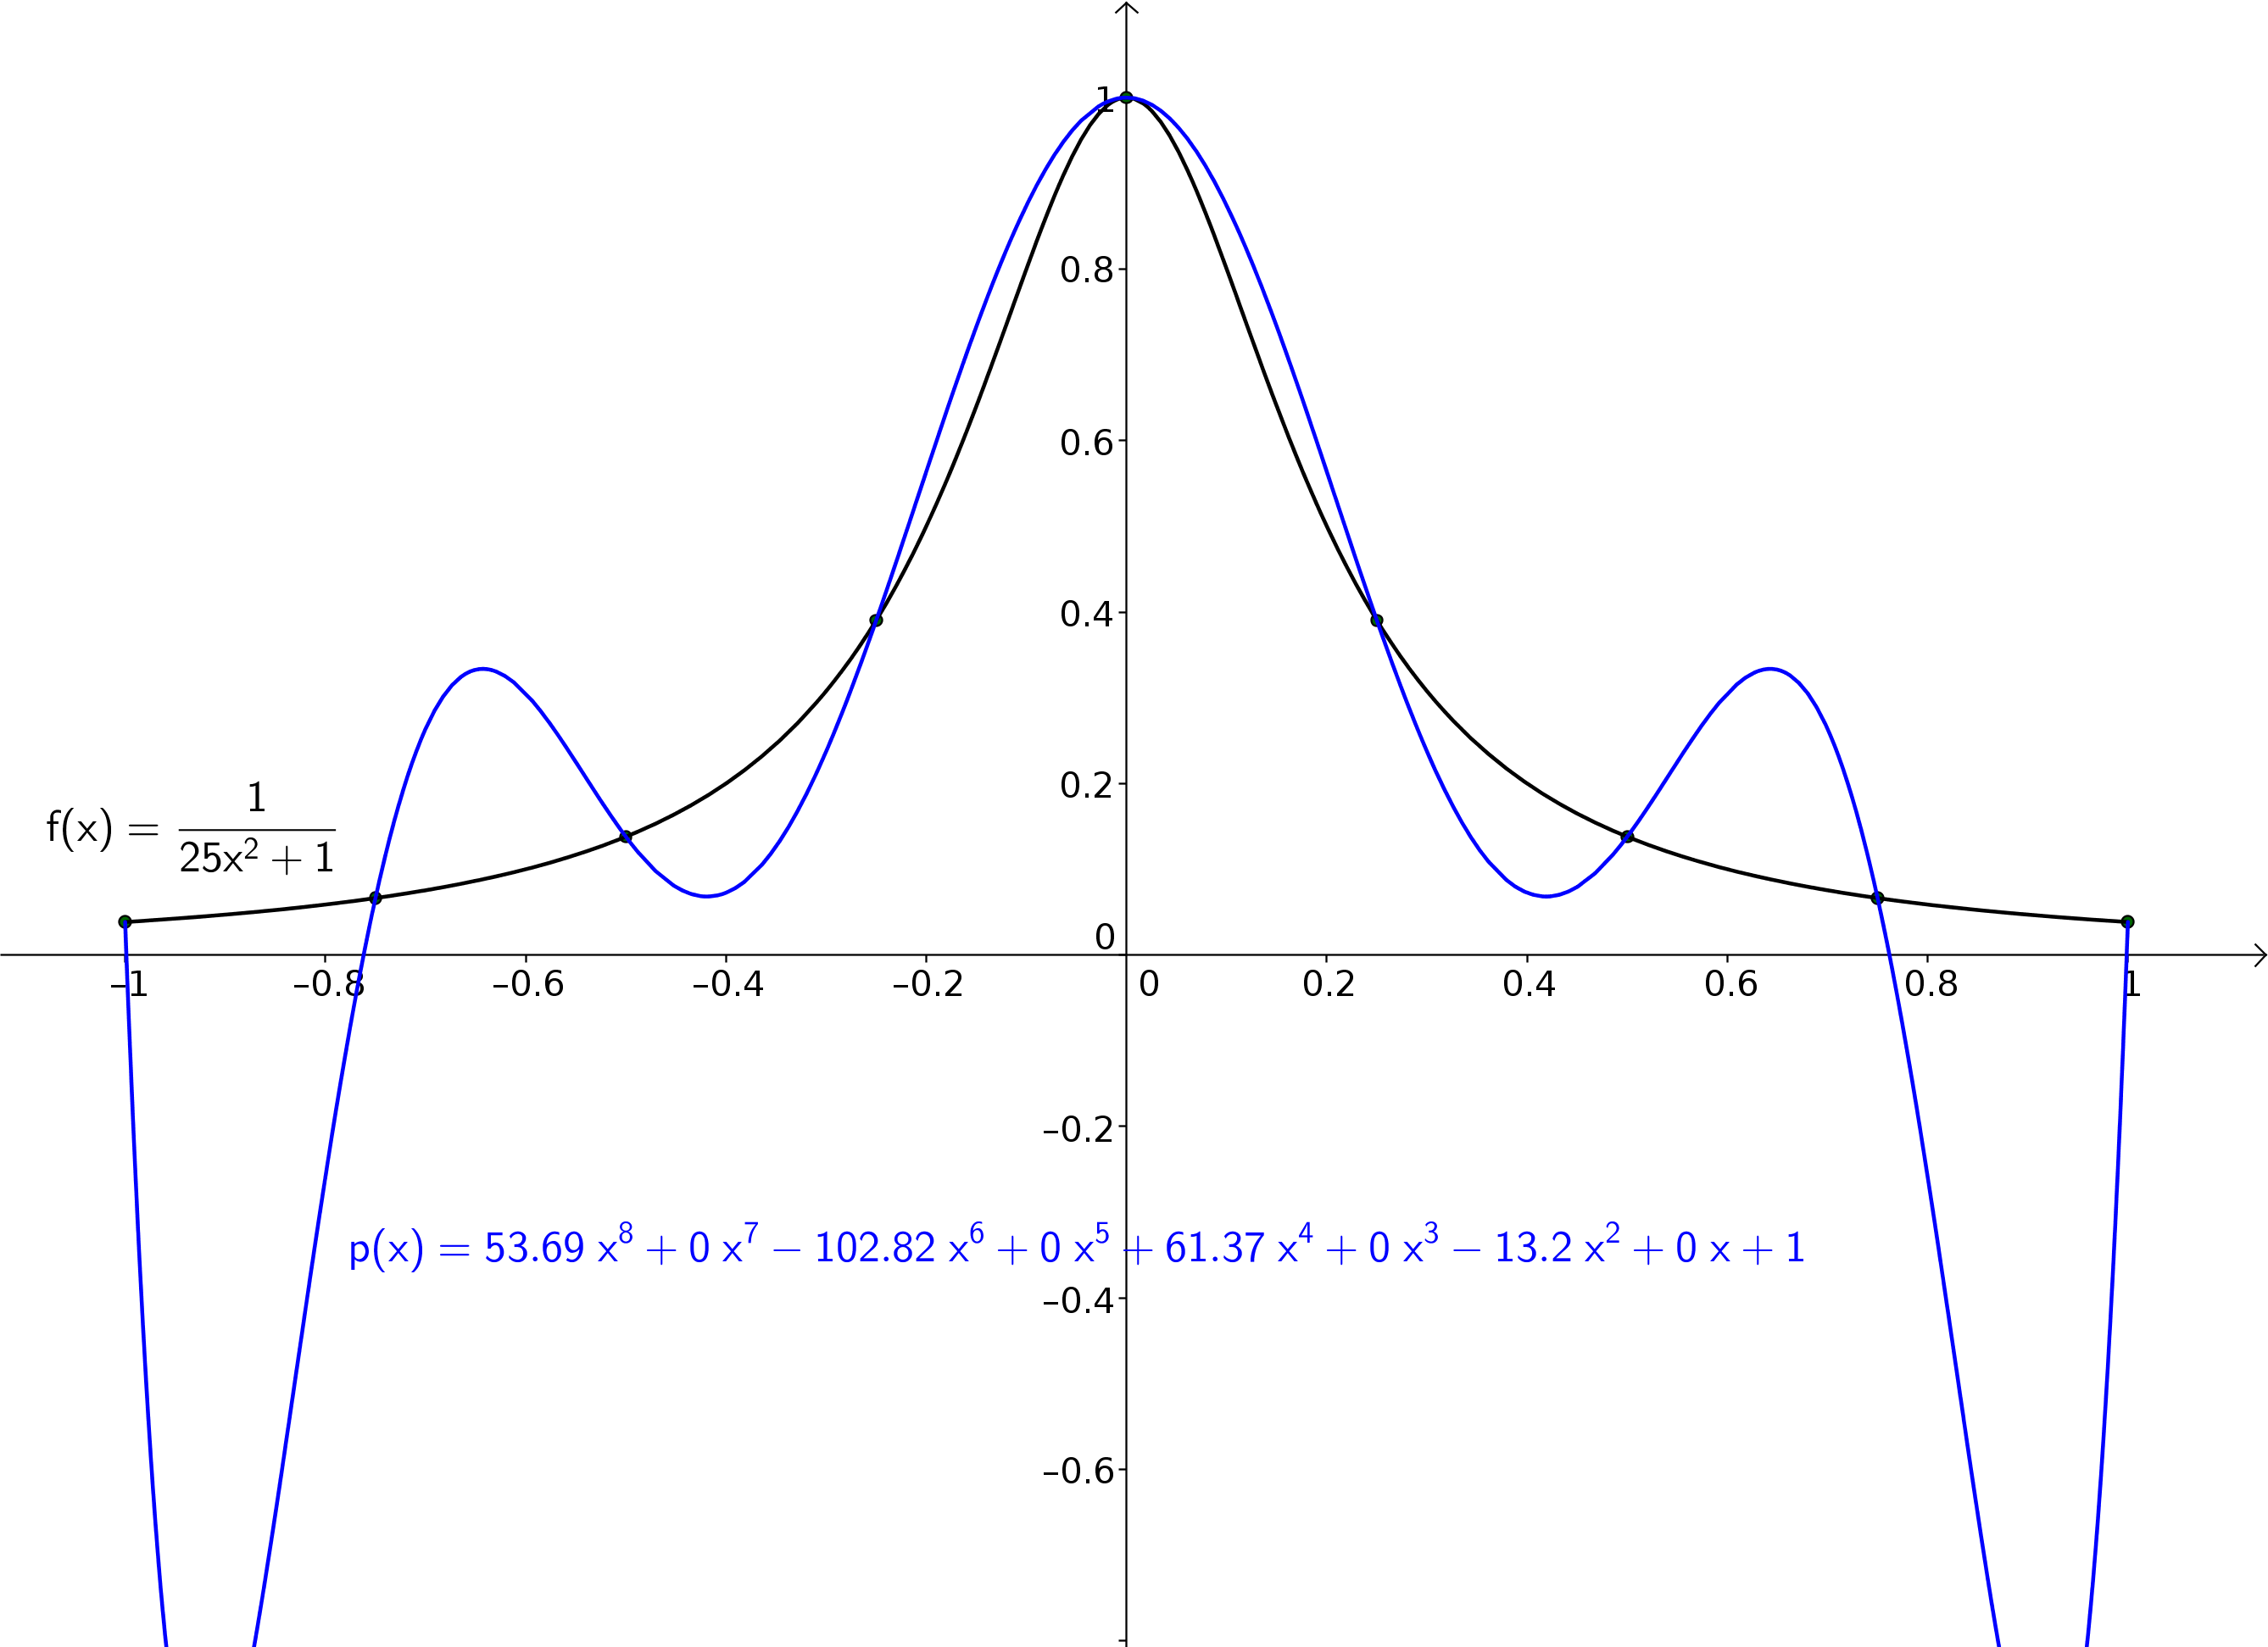
\includegraphics{vond_bruun1.png}

Hér sjáum við ,,þægilegt'' fall þar sem brúunarmargliðan gefur afskaplega
vonda nálgun.


\subsection{Val á brúunarpunktum}
\label{kafli03:val-a-bruunarpunktum}
Það er ekki sjálfgefið að við getum valið í hvaða brúunarpunkta við
notum, t.d. ef þeir ákvarðast af mælingum. Ef við hins vegar getum valið
þá óhindrað, þá vaknar sú spurning hvernig er best að gera það?

\index{staðall!ℓ\(\infty\)}\index{staðall!ℓ2}

\subsection{Skilgreining}
\label{kafli03:index-14}\label{kafli03:skilgreining}
Fyrst þurfum við að útskýra betur hvað við eigum við með ,,best”. Við
munum bara notast við tvær leiðir hér til að mæla skekkjuna, en það er
\(\ell_\infty\) og \(\ell_2\) staðlarnir, fyrir samfellt fall
\(h\) á bilinu \([a,b]\) þá eru þeir skilgreindir með
\begin{gather}
\begin{split}\|h\|_\infty  = \max_{x\in[a,b]} |h(x)|,\end{split}\notag
\end{gather}
og
\begin{gather}
\begin{split}\|h\|_2 = \left( \int_a^b h(x)^2\, dx \right)^\frac 12\end{split}\notag
\end{gather}
\begin{notice}{note}{Athugasemd:}
Það má líta þannig á þetta að \(\ell_\infty\) staðallinn
mæli hámarksskekkju og \(\ell_2\) mæli einhvers konar,,meðaltalsskekkju'',
þar sem meðaltalið er reiknað með heildi.
\end{notice}


\subsection{Verkefnið}
\label{kafli03:verkefni}
Verkefnið er því eftirfarandi: Fyrir gefið fall \(f(x)\) á bili
\([a,b]\) og fast \(n\), þá viljum við finna
\(x_0,\ldots,x_n\) sem lágmarka annað hvort
\begin{gather}
\begin{split}\|f-p\|_\infty \quad \text{ eða } \quad \|f-p\|_2.\end{split}\notag
\end{gather}
Þar sem \(p\) er brúunarmargliðan fyrir brúunarpunktana
\((x_i,f(x_i))\).

Byrjum á að skoða \(\ell_\infty\) tilvikið.

\index{margliður!Chebyshev}

\subsection{Skilgreining: Chebyshev margliður}
\label{kafli03:index-15}\label{kafli03:skilgreining-chebyshev-margliur}
Fyrir náttúrlega tölu \(n\) þá skilgreinum við
\emph{Chebyshev margliðuna} \(T_n\) á \([-1,1]\) með
\begin{gather}
\begin{split}T_n(x) = \cos(n \arccos(x)).\end{split}\notag
\end{gather}
Með því að setja inn \(n=0\) og \(n=1\) þá fæst að
\begin{gather}
\begin{split}T_0(x) = 1 \quad \text{ og } \quad T_1(x) = x,\end{split}\notag
\end{gather}
og með hornafallareglunum fæst að
\begin{gather}
\begin{split}T_{n+1}(x) = 2xT_n(x) - T_{n-1}(x), n \geq 1.\end{split}\notag
\end{gather}
Af jöfnunni hér á undan þá fæst með þrepun að
\begin{itemize}
\item {} 
\(T_n(x)\) er margliða af stigi \(n\).

\item {} 
Forystustuðull \(T_n\) er \(2^{n-1}\).

\item {} 
\(T_n\) er jafnstæð ef \(n\) er slétt og oddstæð ef \(n\)
er oddatala.

\end{itemize}


\subsection{Setning}
\label{kafli03:setning}
Chebyshev margliðan \(T_n\) hefur \(n\) einfaldar
núllstöðvar á bilinu \([-1,1]\) og þær eru gefnar með
\begin{gather}
\begin{split}x_j = \cos\left(\frac{2j+1}{2n}\pi\right),\qquad j=0,1,2,3,\ldots,n-1.\end{split}\notag
\end{gather}
Auk þess eru útgildi \(T_n\) á \([-1,1]\) staðsett í
\begin{gather}
\begin{split}z_j = \cos\left( \frac{j\pi}{n}\right),\qquad j=0,1,2,\ldots,n,\end{split}\notag
\end{gather}
og fallgildin þar uppfylla \(T_n(z_j) = (-1)^j\)

\index{margliður!staðlaðar}

\subsection{Staðlaðar Chebyshev margliður}
\label{kafli03:index-16}\label{kafli03:stalaar-chebyshev-margliur}
Margliða er kölluð \emph{stöðluð} ef forystustuðull hennar er 1.

\emph{Stöðluðu Chebyshev margliðurnar} \(\tilde T\) eru skilgreindar á eftirfarandi hátt
\begin{gather}
\begin{split}\tilde T(x) =
    \begin{cases}
      T_0(x) & \text{ef } n = 0 \\
      2^{1-n}T_n(x)   & \text{ef } n\geq 1              \end{cases}\end{split}\notag
\end{gather}
Fyrir sérhverja staðlaða margliðu \(q\) af stigi
\(n\) þá er
\begin{gather}
\begin{split}\frac 1{2^{n-1}} = \max_{x\in [-1,1]} T_n(x) \leq \max_{x\in[-1,1]} |q(x)|.\end{split}\notag
\end{gather}
Þ.e. af öllum stöðluðum margliðum þá eru stöðluðu Chebyshev margliðurnar
,,minnstar” á bilinu \([-1,1]\).


\subsection{Skynsamlegir skiptipunktar fyrir bilið \([-1,1]\)}
\label{kafli03:skynsamlegir-skiptipunktar-fyrir-bili}
Við vitum að skekkjan í því að nálga fallið \(f\) með
brúunarmargliðu \(p\) með brúunarpunkta \(x_0,\ldots,x_n\) er
\begin{gather}
\begin{split}f(x)-p(x) = \frac{f^{(n+1)}(\xi)}{(n+1)!}\, (x-x_0)(x-x_1)\cdots (x-x_n),\end{split}\notag
\end{gather}
þar sem \(\xi\) er á minnsta bilinu sem inniheldur \(x\) og
\(x_0,x_1,\ldots,x_n\). Ef við skoðum jöfnuna að ofan þá sjáum við
að þar sem \(n\) og \(f\) (og þar með \(f^{(n+1)}\)) er fast
þá er stæðan \((x-x_0)\cdots(x-x_n)\) það eina sem við höfum
einhverja stjórn á.

Með því að nota Chebyshev margliðurnar þá getum við lágmarkað þennan
hluta skekkjunnar.

Athugið að \((x-x_0)\cdots (x-x_n)\) er stöðluð margliða af stigi
\(n+1\). Þannig að samkvæmt því sem kom fram hér að
ofan þá lágmörkum við framlag hennar
til skekkjunnar með \((x-x_0)\cdots (x-x_n) = \tilde T_{n+1}\),
þ.e. með því að velja
\begin{gather}
\begin{split}x_i = \cos\left(\frac{2i+1}{2(n+1)}\pi\right), \qquad i=0,1,\ldots,n.\end{split}\notag
\end{gather}
Hæsta gildi \(\tilde T_{n+1}\) er \(\frac 1{2^n}\), sem þýðir að
við fáum skekkjumatið
\begin{gather}
\begin{split}\|f(x)-p(x)\|_\infty \leq \frac{\|f^{(n+1)}\|_\infty}{2^n(n+1)!}.\end{split}\notag
\end{gather}

\subsection{Dæmi um óheppilega skiptipunkta skoðað aftur}
\label{kafli03:daemi-um-oheppilega-skiptipunkta-skoa-aftur}
Skoðum aftur fallið \(f(x) = 1/(25x^2+1)\), en í stað þess að taka 9
jafndreifaða brúunarpunkta á bilinu \([-1,1]\), þá skulum við nota
Chebyshev margliðurnar til að finna 9 punkta á bilinu.

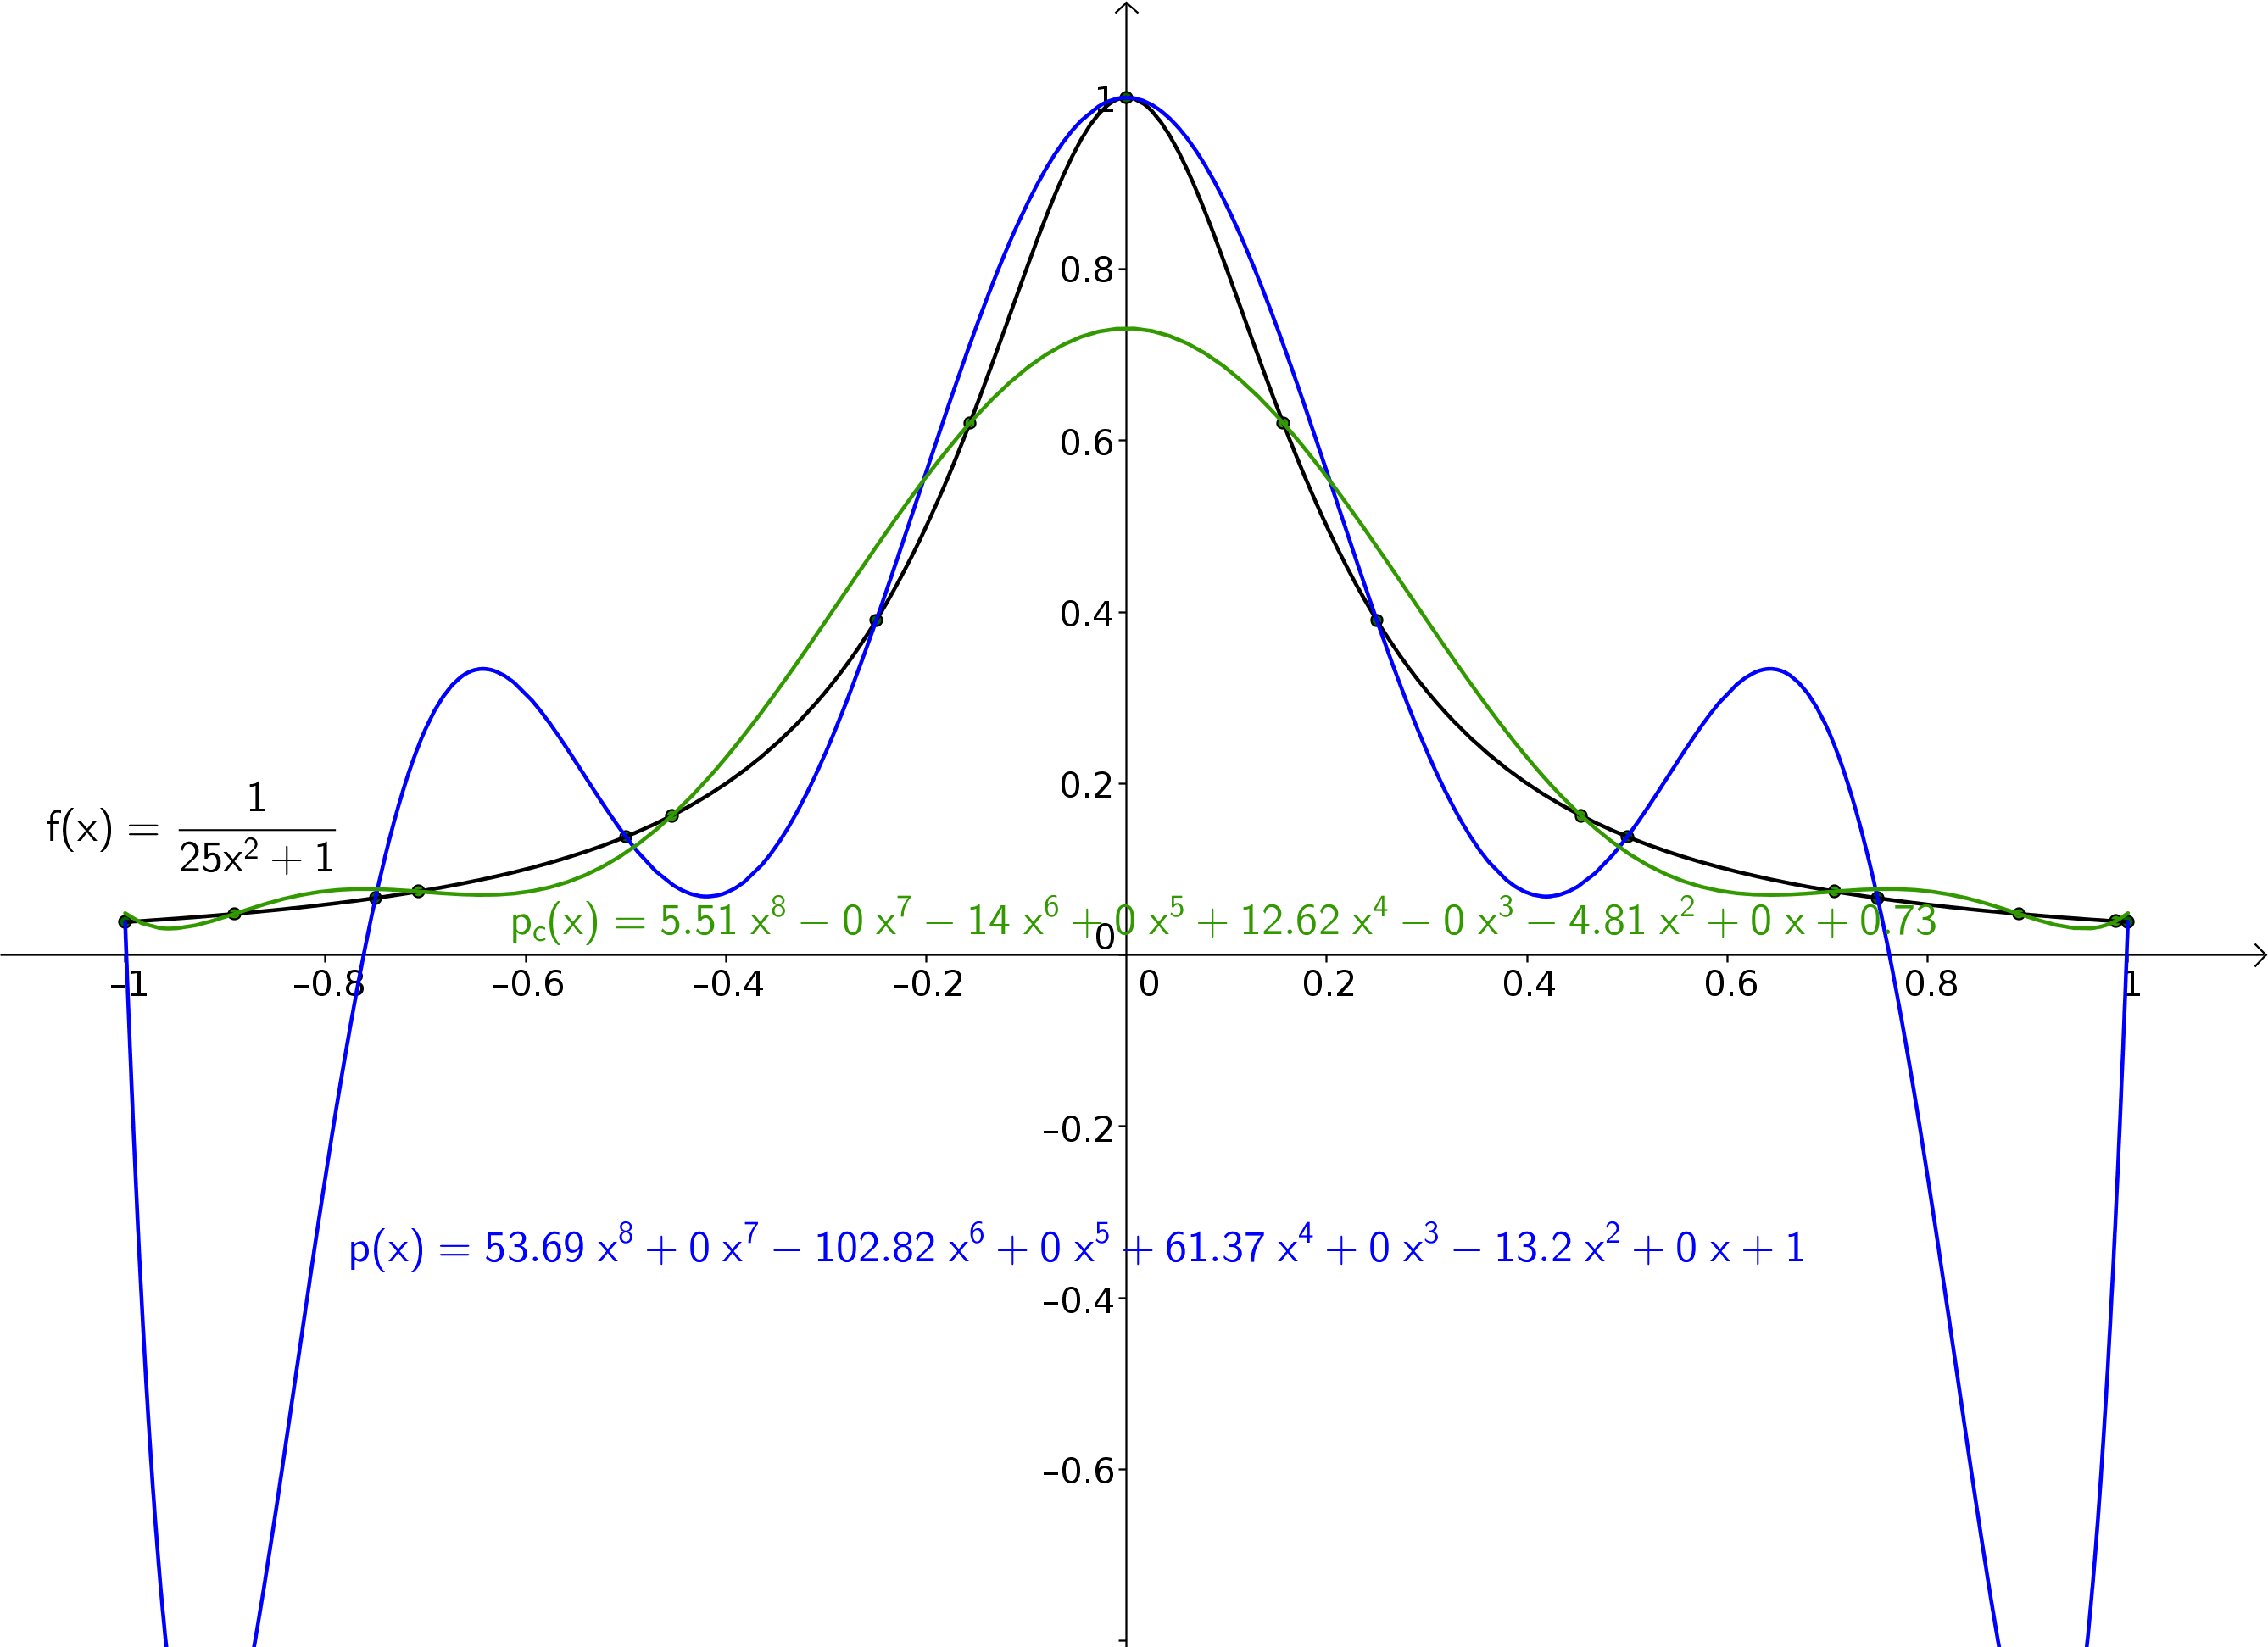
\includegraphics{vond_bruun2.png}


\subsection{Skynsamlegir skiptipunktar fyrir bil \([a,b]\)}
\label{kafli03:skynsamlegir-skiptipunktar-fyrir-bil}
Hér á undan miðaðist allt við að finna brúunarmargliðu fyrir fallið
\(f\) á bilinu \([-1,1]\). Ef við viljum skoða almennt bil
\([a,b]\) þá byrjum við á athuga að fallið
\(\eta:[-1,1]\to [a,b]\),
\begin{gather}
\begin{split}\eta(t) = \frac{b-a}2 t + \frac{b+a}2\end{split}\notag
\end{gather}
skilgreinir línulega vörpun (hliðrun og stríkkun) frá \([-1,1]\)
yfir á \([a,b]\). Athugið að vörpunin sendir \(-1\) í \(a\)
og \(1\) í \(b\).

Með því að taka rætur stöðluðu Chebyshev margliðunnar
\(\tilde T_{n+1}\) og varpa þeim með \(\eta\) yfir á bilið
\([a,b]\) þá fáum við þá punkta \(x_0,\ldots,x_n \in [a,b]\) sem
lágmarka \((x-x_0)\cdots (x-x_n)\) á bilinu \([a,b]\),
\begin{gather}
\begin{split}x_i = \eta\left(\cos\left(\frac{2i+1}{2(n+1)}\pi\right)\right)
    = \frac{b-a}2 \cos\left(\frac{2i+1}{2(n+1)}\pi\right) + \frac{b+a}2,\end{split}\notag
\end{gather}
\(i=0,1,2,\ldots,n\).


\subsection{Lágmörkun á skekkju með tilliti til \(\ell_2\)}
\label{kafli03:lagmorkun-a-skekkju-me-tilliti-til}
Nú skulum við skipta um staðal, þannig að í stað þess að lágmarka
\(\|f-p\|_\infty\) þá skulum við reyna að lágmarka
\begin{gather}
\begin{split}\|f-p\|_2 = \left(\int_a^b (f-p)^2\, dx\right)^{1/2}\end{split}\notag
\end{gather}
Við vitum að skekkjan í því að nálga fallið \(f\) með
brúunarmargliðu \(p\) með brúunarpunkta \(x_0,\ldots,x_n\) er
\begin{gather}
\begin{split}f(x)-p(x) = \frac{f^{(n+1)}(\xi)}{(n+1)!}\, (x-x_0)(x-x_1)\cdots (x-x_n),\end{split}\notag
\end{gather}
þar sem \(\xi\) er á minnsta bilinu sem inniheldur \(x\) og
\(x_0,x_1,\ldots,x_n\).

Eins og áður þá sjáum við að stæðan \((x-x_0)\cdots(x-x_n)\) það
eina sem við getum stjórnað með því að velja brúunarpunktana
\(x_j\).

\index{margliður!Legendre}

\subsection{Skilgreining: Legendre margliðurnar}
\label{kafli03:index-17}\label{kafli03:skilgreining-legendre-margliurnar}
Fyrir náttúrlega tölu \(n\) þá skilgreinum við
\emph{Legendre margliðurnar} svona
\begin{gather}
\begin{split}\begin{aligned}
   P_0(x) &= 1,\\
   P_1(x) &= x,\\
   P_n(x) &= \frac{2n-1}n x P_{n-1}(x) - \frac{n-1}n P_{n-2}(x).
  \end{aligned}\end{split}\notag
\end{gather}
Af skilgreiningunni hér á undan þá sjáum við að
\begin{itemize}
\item {} 
\(P_n(x)\) er margliða af stigi \(n\).

\item {} 
Forystustuðull \(P_n\) er
\(\frac {2n-1}n \cdot \frac {2n-3}{n-2} \cdots \frac 32 \cdot 1\).

\item {} 
\(P_n\) er jafnstæð ef \(n\) er slétt og oddstæð ef \(n\)
er oddatala.

\end{itemize}


\subsection{Setning}
\label{kafli03:id5}\begin{gather}
\begin{split}\int_{-1}^1 P_j(x) P_k(x)\, dx =
    \begin{cases}
     0, & \text{ef } j\neq k\\
     \frac{2}{2j+1}, & \text{ef } j=k.
    \end{cases}\end{split}\notag
\end{gather}
Einnig gildir að ef \(q\) er margliða af stigi minna en \(n\) þá er
\begin{gather}
\begin{split}\int_{-1}^1 q(x)P_n(x)\, dx = 0.\end{split}\notag
\end{gather}
Þetta segir okkur að Legendre margliðurnar eru hornréttar (með tilliti
til innfeldisins sem heildið skilgreinir).


\subsection{Setning}
\label{kafli03:id6}
\(P_n\) hefur \(n\) ólíkar núllstöðvar sem liggja
allar á \([-1,1]\).


\subsection{Skilgreining: Staðlaðar Legendre margliður}
\label{kafli03:skilgreining-stalaar-legendre-margliur}
Eins og þegar við fengumst við Chebyshev margliðurnar þá skilgreinum við
\emph{stöðluðu Legendre margliðurnar} \(\tilde P_n\) með því að deila upp
í \(P_n\) með forrystustuðlunum \(P_n\).

\begin{notice}{note}{Athugasemd:}
Setningarnar þrjár hér undan gilda um \(\tilde P\) alveg eins og \(P\).
\end{notice}


\subsection{Setning: Lágmörkun með Legendre margliðunum}
\label{kafli03:setning-lagmorkun-me-legendre-margliunum}
Ef \(p\) er stöðluð margliða af stigi \(n+1\) þá er
\(\|p\|_2\geq \|\tilde P_{n+1}\|_2\).

Skilgreinum
\(q = p-\tilde P_{n+1}\), sem þýðir að \(q\) er margliða af
stigi minna en \(n+1\). Nú er
\begin{gather}
\begin{split}\begin{aligned}
   \|p\|_2^2 &= \|\tilde P_{n+1} + q\|_2^2 \\
   &= \int_{-1}^1 (\tilde P_{n+1}(x) + q(x))^2\, dx \\
   &= \int_{-1}^1 \tilde P_{n+1}(x)^2 + 2q(x)\tilde P_{n+1}(x) + q(x)^2\, dx\\
   &= \|\tilde P_{n+1}\|_2^2 + 2\int_{-1}^1 q(x)\tilde P_{n+1}(x)\, dx + \|q\|_2^2\\
   &= \|\tilde P_{n+1}\|_2^2 +  \|q\|_2^2 \geq \|\tilde P_{n+1}\|_2^2
  \end{aligned}\end{split}\notag
\end{gather}
því \(\int_{-1}^1 q(x)\tilde P_{n+1}(x)\, dx=0\) og
\(\|q\|_2 \geq 0\).

Af síðustu setningu sjáum við að til þess að lágmarka
\begin{gather}
\begin{split}\|f(x)-p(x)\|_2 = \left\|\frac{f^{(n+1)}(\xi)}{(n+1)!}\, (x-x_0)(x-x_1)\cdots (x-x_n) \right\|_2,\end{split}\notag
\end{gather}
þá veljum við \(x_1,\ldots,x_n\) þannig að
\((x-x_0)(x-x_1)\cdots (x-x_n) = \tilde P_{n+1}\).
Þ.e. \(x_j\) þurfa að vera rætur stöðluðu Legendre margliðunnar af
stigi \(n+1\).


\subsection{Núllstöðvar \(P_n\), fyrir \(n=1,\ldots,10\)}
\label{kafli03:nullstovar-fyrir}
Ólíkt Chebyshev margliðunum þá er ekki hlaupið að því að finna rætur
\(\tilde P_{n+1}\). Þannig að við þurfum að reikna þær tölulega og
geyma í töflu.

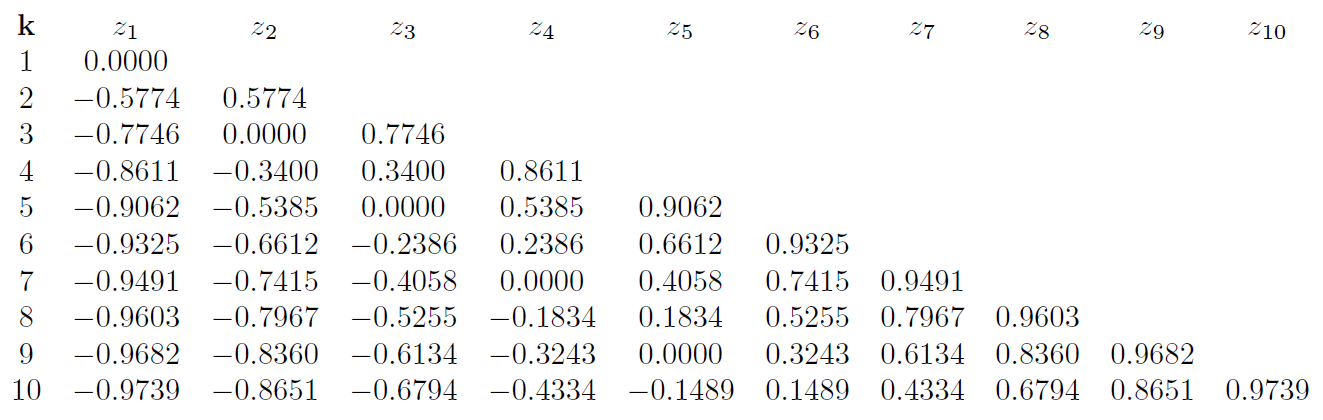
\includegraphics{legendre.png}


\subsection{Dæmi um óheppilega skiptipunkta skoðað aftur}
\label{kafli03:id7}
Skoðum enn einu sinni fallið \(f(x) = 1/(25x^2+1)\), en í stað þess
að taka 9 jafndreifaða brúunarpunkta á bilinu \([-1,1]\), þá skulum
við nota Legendre margliðurnar til að finna 9 punkta á bilinu.

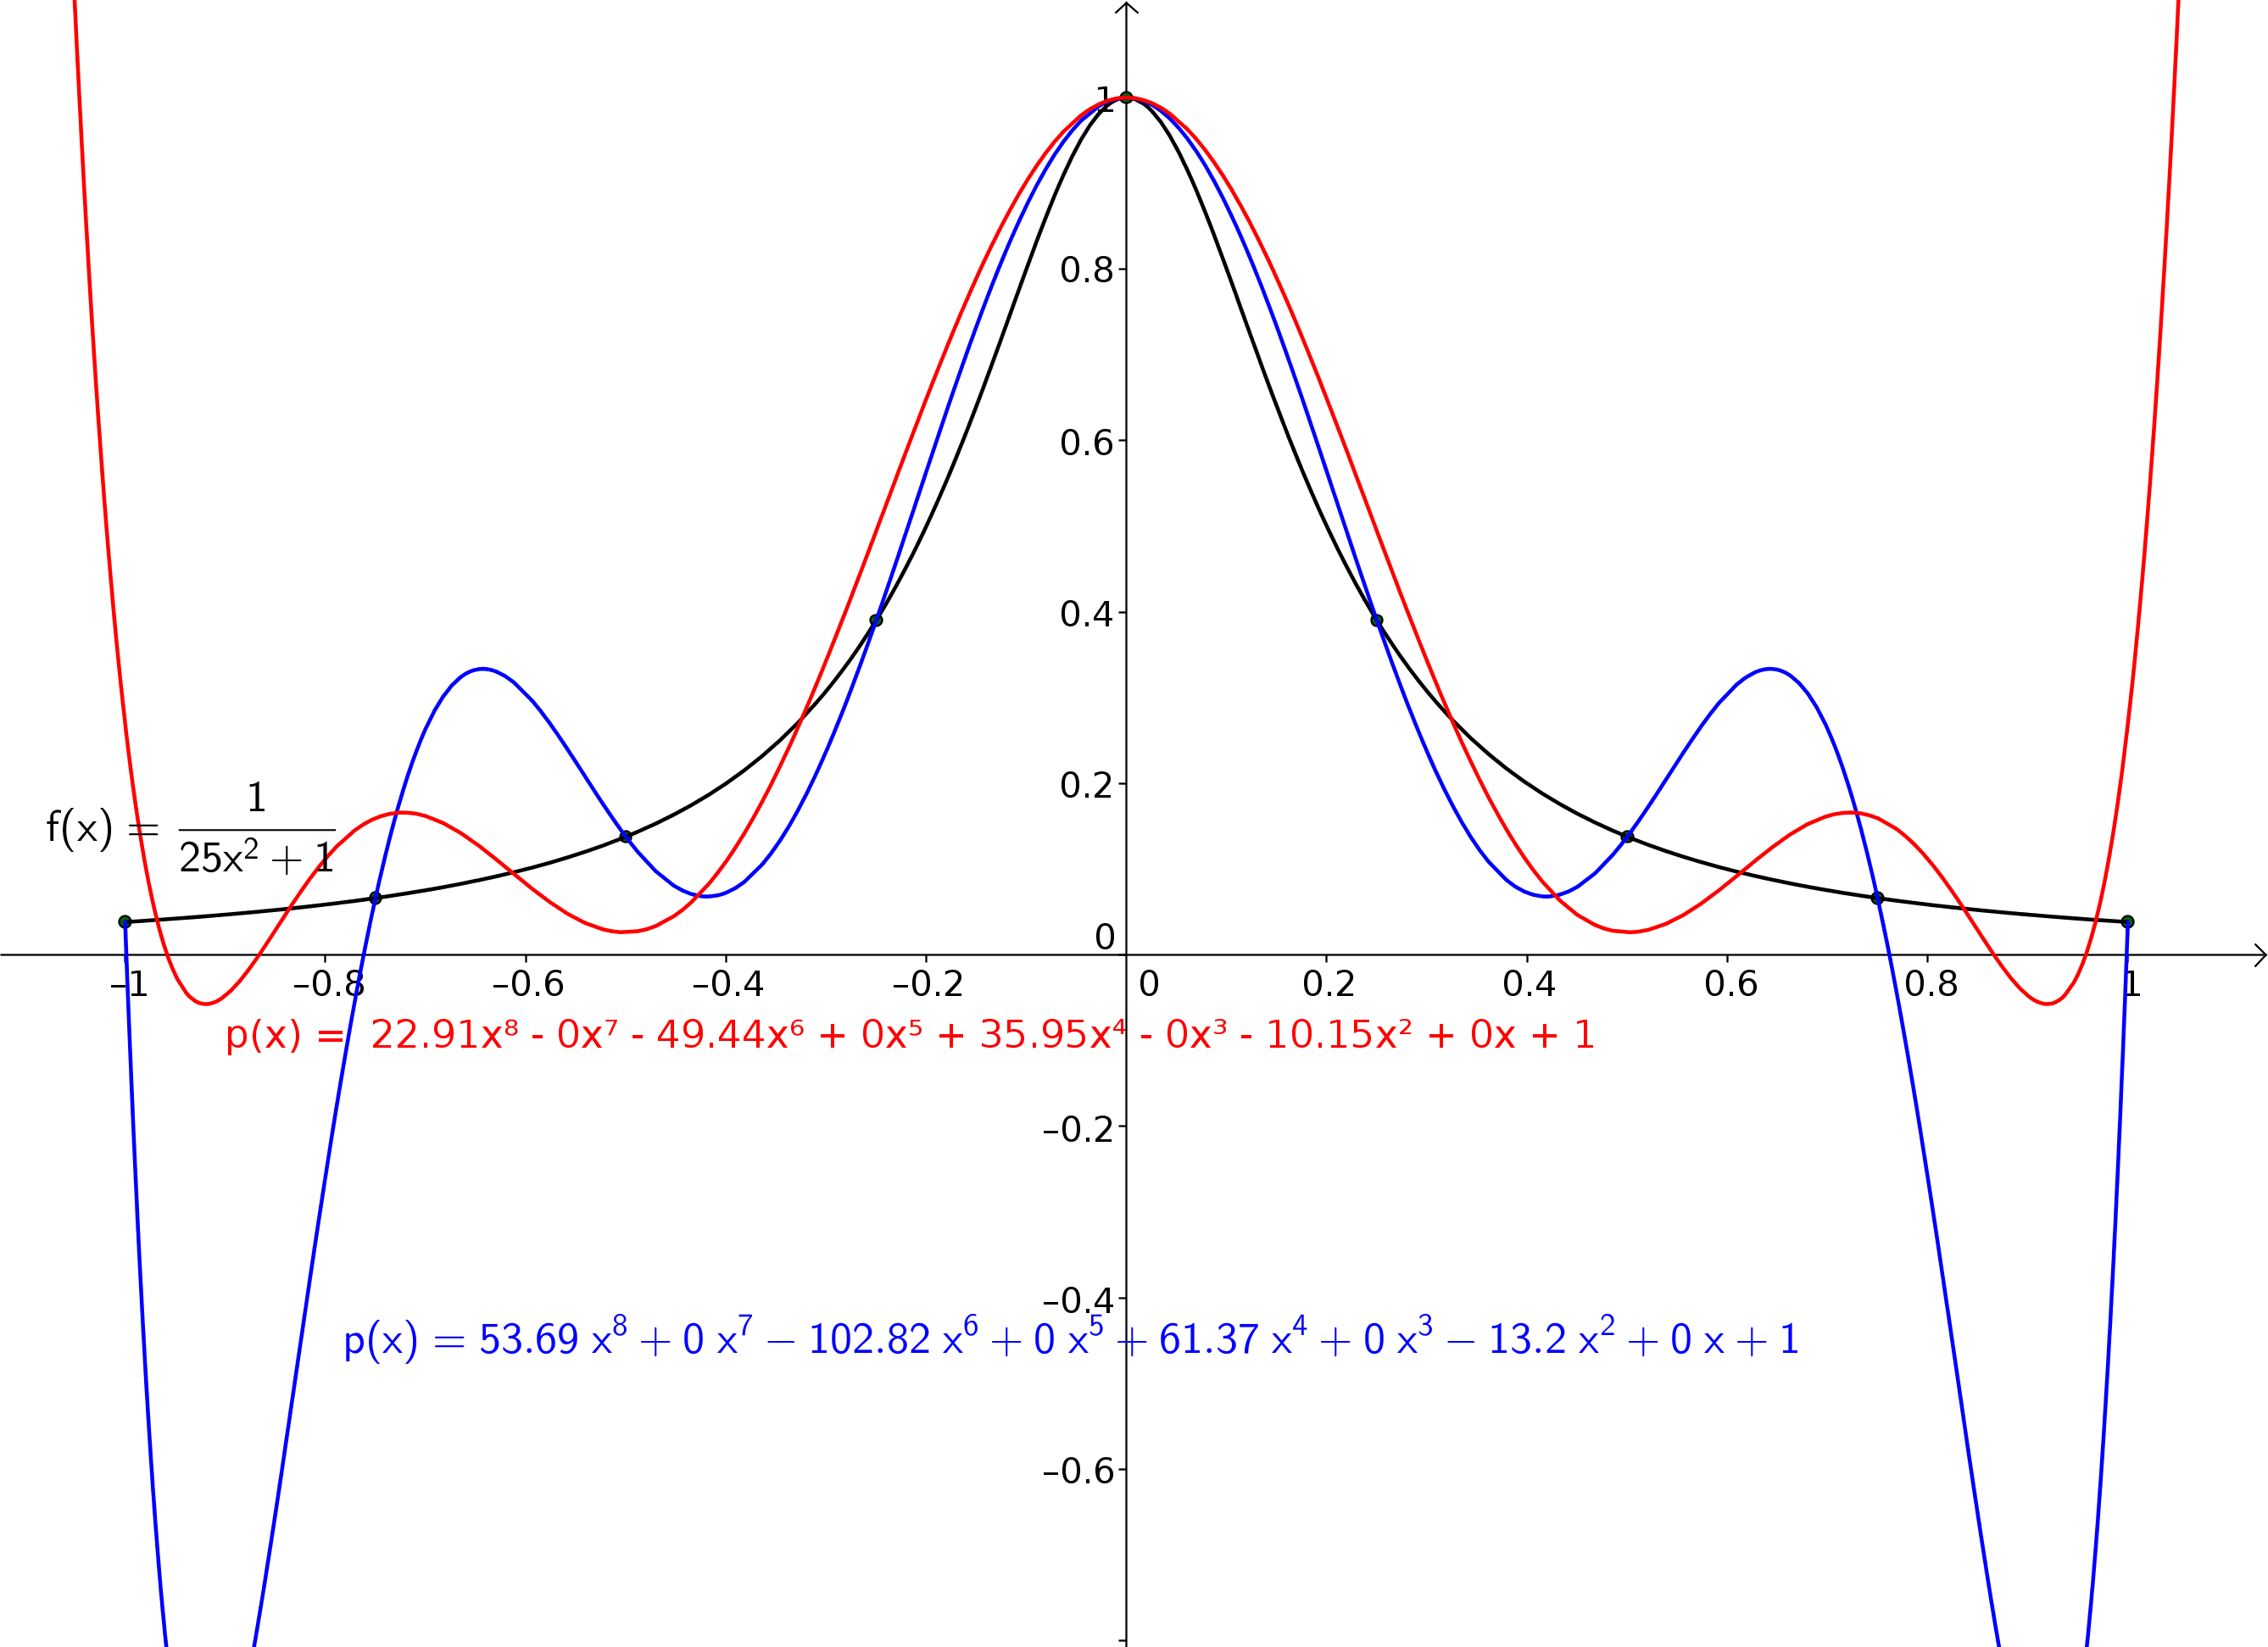
\includegraphics{vond_bruun3.png}


\subsection{Athugasemd um \(\ell_\infty\) og \(\ell_2\)}
\label{kafli03:athugasemd-um-og}
\begin{notice}{note}{Athugasemd:}
Það má líta þannig á þetta að \(\ell_\infty\) staðallinn
mæli hámarksskekkju
og \(\ell_2\) mæli einhvers konar,,heildarskekkju'',
þar sem skekkjan er reiknað með heildinu hér á undan og svarar því hér um
bil til flatarmálsins á milli fallsins og brúunarmargliðunnar.
\end{notice}
\begin{itemize}
\item {} 
\(\ell_\infty\) staðallinn mælir hámarksskekkju, þannig að með
því nota Chebyshev margliðurnar þá erum við að reyna að lágmarka mestu skekkju
á bilinu.

\item {} 
\(\ell_2\) mæli einhvers konar,,heildarskekkju'',
þar sem skekkjan er reiknað með heildi.
Þannig að með því að nota Legendre margliðurnar þá erum við
í einhverjum skilningi að lágmarka flatarmál.

\end{itemize}

\index{brúun!skekkjumat}

\section{Skekkjumat}
\label{kafli03:index-18}\label{kafli03:skekkjumat}

\subsection{Nálgun á föllum með margliðum}
\label{kafli03:nalgun-a-follum-me-marglium}
Lítum nú aftur á almenna brúunarverkefnið og gefum okkur að tölurnar
\(y_i^{(j)}\) séu af gerðinni \(f^{(j)}(a_i)\) þar sem
\(f : I \to {{\mathbb  R}}\) er fall á bili \(I\) sem inniheldur
alla punktana \(a_1, \ldots, a_k\).

Þá snýst brúunarverkefnið um að finna margliðu af stigi \(\leq m\)
sem uppfyllir
\begin{gather}
\begin{split}p^{(j)}(a_i) = f^{(j)}(a_i), \quad
  j = 0, \ldots, m_i-1, \quad i = 1, \ldots, k.\end{split}\notag
\end{gather}
Við vitum að lausn þess er ótvírætt ákvörðuð. Ef við notum Newton form
lausnarinnar, þá táknum við mismunakvótana með
\begin{gather}
\begin{split}f[x_i,\ldots,x_{i+j}]\end{split}\notag
\end{gather}
í stað
\begin{gather}
\begin{split}y[x_i,\ldots,x_{i+j}]\end{split}\notag
\end{gather}

\subsection{Nálgun á fallgildum}
\label{kafli03:nalgun-a-fallgildum}
Runurnar \((x_0,\ldots,x_m)\) og \((y_0,\ldots,y_m)\) eru
skilgreindar með
\begin{gather}
\begin{split}(x_0,x_1,\ldots,x_m) =
  (\underbrace{a_1, \ldots, a_1}_{m_1 \, \text{sinnum}},
  \underbrace{a_2, \ldots , a_2}_{m_2 \, \text{sinnum}},
  \ldots ,
  \underbrace{a_k, \ldots , a_k}_{m_k \, \text{sinnum}})\end{split}\notag
\end{gather}
og
\begin{gather}
\begin{split}\begin{gathered}
  (y_0,y_1,\ldots,y_m) =
  (f^{(0)}(a_1), \ldots, f^{(m_1-1)}(a_1),
f^{(0)}(a_2), \ldots, f^{(m_2-1)}(a_2) \\ \ldots,
  f^{(0)}(a_k), \ldots, f^{(m_k-1)}(a_k))
  \label{bru.margfald.5}\end{gathered}\end{split}\notag
\end{gather}

\subsection{Skekkjumat}
\label{kafli03:id8}
Nú tökum við punkt \(x \in I\) og spyrjum um skekkjuna
\(f(x) - p(x)\) í nálgun á \(f(x)\) með \(p(x)\). Ef
\(x\) er einn punktana \(a_1, \ldots, a_k\), þá er
\(p(x) = f(x)\) og skekkjan þar með 0, svo við skulum gera ráð fyrir
að \(x \not= a_i\), \(i = 1, \ldots, k\).

Við bætum nú \((x,f(x))\) sem einföldum brúunarpunkti við alhæfða
brúunar verkefnið og fáum sem lausn \(q(t)\) á þessu aukna verkefni.
Margliðan \(q\) er af stigi \(\leq m+1\). Við notum táknið
\(t\) fyrir breytu, því \(x\) er frátekið.

Þá uppfyllir \(q(t)\) að \(q(x) = f(x)\) auk allra skilyrðanna
\begin{gather}
\begin{split}q^{(j)}(a_i) = p^{(j)}(a_i) = f^{(j)}(a_i)\end{split}\notag
\end{gather}
í verkefninu sem við byrjuðum með.

Við getum þá skrifað (sjá \emph{Newton-margliður} til hliðsjónar)
\begin{gather}
\begin{split}\begin{aligned}
  q(t) &= p(t) + f[x_0,\ldots,x_m,x](t-x_0)\cdots(t-x_m) \\
  &= p(t) + f[x_0,\ldots,x_m,x](t-a_1)^{m_1}\cdots(t-a_k)^{m_k}.\end{aligned}\end{split}\notag
\end{gather}
Þegar við gefum breytunni \(t\) gildið \(x\), þá fáum við
\(q(x) = f(x)\) og því fæst formúla fyrir skekkjunni
\begin{gather}
\begin{split}f(x) - p(x)
  = f[x_0,\ldots,x_m,x](x-a_1)^{m_1}\cdots(x-a_k)^{m_k}\end{split}\notag
\end{gather}
Nú ætlum við að finna leið til þess að meta skekkjuliðinn. Til þess
þurfum við að gefa okkur að \(f\) hafi að minnsta kosti \(m+1\)
afleiðu.


\subsection{Tilfellið þegar við höfum aðeins einn punkt}
\label{kafli03:tilfelli-egar-vi-hofum-aeins-einn-punkt}
Munum nú að í tilfellinu þegar við erum bara með einn punkt \(a_1\),
þá erum við með \(m+1\) skilyrði
\begin{gather}
\begin{split}p^{(j)}(a_1)=f^{(j)}(a_1), \qquad j=0,\dots,m\end{split}\notag
\end{gather}
og við fáum að \(p\) er Taylor-margliða fallsins \(f\) í
punktinum \(a_1\). Þá er \(x_0=\cdots=x_m=a_1\) og við fáum
\begin{gather}
\begin{split}f(x) - p(x)
  = f[x_0,\ldots,x_m,x](x-a_1)^{m+1}\end{split}\notag
\end{gather}
Nú segir setning Taylors okkur að til sé punktur \(\xi\) milli
\(a_1\) og \(x\) þannig að
\begin{gather}
\begin{split}f(x) - p(x)
  = \dfrac{f^{(n+1)}(\xi)}{(n+1)!}(x-a_1)^{m+1}\end{split}\notag
\end{gather}
Við getum því dregið þá ályktun að í þessu sértilfelli er
\begin{gather}
\begin{split}f[x_0,\ldots,x_m,x]=\dfrac{f^{(n+1)}(\xi)}{(n+1)!}\end{split}\notag
\end{gather}
Það kemur í ljós að þetta er almenn regla sem gildir fyrir \emph{öll}
alhæfðu brúunarverkefnin.

\textbf{Tilfellið} \(m=1\) \textbf{er meðalgildisreglan}

Munum að tilfellið \(m=1\) er meðalgildisreglan
\begin{gather}
\begin{split}f[a_1,x]=\dfrac{f(x)-f(a_1)}{x-a_1}=f'(\xi).\end{split}\notag
\end{gather}

\subsection{Margfeldni núllstöðva}
\label{kafli03:margfeldni-nullstova}
Samfellt fall \(\varphi\) á bili \(I\) er sagt hafa núllstöð \emph{af
stigi að minnsta kosti} \(m>0\) í punktinum \(a\in I\), ef til
er samfellt fall \(\psi\) á \(I\) þannig að
\begin{gather}
\begin{split}\varphi(x)=(x-a)^m\psi(x)\end{split}\notag
\end{gather}
Við segjum að \(\varphi\) hafi núllstöð af \emph{margfeldni} \(m\) ef
\(\psi(a)\neq0\).

Athugið að ef \(\varphi\) er deildanlegt \(I\) með samfellda
afleiðu, þá er \(\psi\) deildanlegt með samfellda afleiðu í
\(I\setminus\{a\}\) og við höfum
\begin{gather}
\begin{split}\begin{aligned}
  \varphi'(x)&=m(x-a)^{m-1}\psi(x)+(x-a)^m\psi'(x)\\
&= (x-a)^{m-1} \big(m\psi(x)+(x-a)\psi'(x)\big)\end{aligned}\end{split}\notag
\end{gather}
Ef afleiðan \(\psi'\) er takmörkuð í grennd um \(a\), þá sjáum
við á þessari formúlu að \(\varphi'\) hefur núllstöð af stigi að
minnsta kosti \(m-1\) í \(a\).

Hugsum okkur nú að við séum með \(a_1,\dots,a_k\) ólíka punkta í
bilinu \(I\) og að \(m_1,\dots,m_k\) séu jákvæðar náttúrlegar
tölur.

Ef fallið \(\varphi\) hefur núllstöðvar í öllum punktunum
\(a_j\) og núllstöðin \(a_j\) er af stigi að minnsta kosti
\(m_j\). Við segjum að þá hafi \(\varphi\) \emph{að minnsta kosti}
\begin{gather}
\begin{split}n=m_1+\cdots+m_k\end{split}\notag
\end{gather}
\emph{núllstöðvar taldar með margfeldni}.

Eins þá segjum við að \(\varphi\) hafi \(n\) núllstöðvar í
\(\{a_1,\dots,a_k\}\) \emph{taldar með margfeldni} ef \(\varphi\)
hefur núllstöðvar í öllum punktum \(a_1,\dots,a_k\) og samanlögð
margfeldni þeirra er \(n\)

Hugsum okkur nú að fallið \(\varphi\) hafi núllstöð af stigi
\(m_j\) í punktunum \(a_j\) fyrir öll \(j=1,\dots,k\) og að
\(n=m_1+\cdots+m_k\).

Til einföldunar gerum við ráð fyrir að
\begin{gather}
\begin{split}a_1<a_2<\cdots<a_k.\end{split}\notag
\end{gather}
Þá gefur meðalgildissetningin að \(\varphi'\) hefur að minnsta kosti
eina núllstöð á sérhverju bilanna
\begin{gather}
\begin{split}]a_1,a_2[, \  ]a_2,a_3[, \ \dots \  ]a_{k-1},a_k[\end{split}\notag
\end{gather}
Þau eru samanlagt \(k-1\) talsins. Að auki vitum við að
\(\varphi'\) hefur núllstöðvar af stigi að minnsta kosti
\(m_j-1\) í punktinum \(a_j\). Ef við leggjum þetta saman, þá
fáum við að \(\varphi'\) hefur núllstöðvar af margfeldni að minnsta
kosti
\begin{gather}
\begin{split}k-1+(m_1-1)+\cdots+(m_k-1)=n-1\end{split}\notag
\end{gather}
í minnsta lokaða bilinu sem inniheldur alla punktana
\(a_1,\dots,a_k\).


\subsection{Setning: Skekkjumat}
\label{kafli03:setning-skekkjumat}
Nú ætlum við að sýna fram á að fyrir föll \(f\) sem eru
\((m+1)\) sinnum samfellt deildanleg að til sé \(\xi\) á minnsta
bili sem inniheldur \(a_1, \ldots, a_k\) og \(x\) þannig að
\begin{gather}
\begin{split}f[x_0,\ldots,x_m,x] = \frac{f^{(m+1)}(\xi)}{(m+1)!}\end{split}\notag
\end{gather}
Við skilgreinum fallið
\begin{gather}
\begin{split}g(t) = f(t) - p(t) - \lambda w(t),\end{split}\notag
\end{gather}
þar sem
\begin{gather}
\begin{split}w(t) = (t-a_1)^{m_1} \cdots (t-a_k)^{m_k}\end{split}\notag
\end{gather}
og talan \(\lambda\) er valin þannig að \(g(x) = 0\).

Nú er \(p^{(j)}(a_i)=f^{(j)}(a_i)\) fyrir \(j=0,\dots,m_i-1\),
þá gefur setning Taylors okkur að \(g\) hefur núllstöð af stigi
\(m_i\) í sérhverjum punktanna \(a_i\). Auk þess hefur \(g\)
núllstöð í \(x\). Samanlagt eru þetta að minnsta kosti \(m+2\)
núllstöðvar taldar með margfeldni.

Höfum:
\begin{itemize}
\item {} 
\(g\) hefur að minnsta kosti \(m+2\) núllstöðvar taldar með margfeldni,

\item {} 
\(g'\) hefur að minnsta kosti \(m+1\) núllstöð talda með margfeldni,

\item {} 
\(g''\) hefur að minnsta kosti \(m\) núllstöðvar taldar með margfeldni

\item {} 
og þannig áfram, þar til við ályktum að

\item {} 
\(g^{(m+1)}\) hefur að minnsta kosti eina núllstöð.

\end{itemize}

Tökum eina slíka og köllum hana \(\xi\).

Munum að
\begin{gather}
\begin{split}g(t) = f(t) - p(t) - \lambda w(t),\end{split}\notag
\end{gather}
þar sem
\begin{gather}
\begin{split}w(t) = (t-a_1)^{m_1} \cdots (t-a_k)^{m_k}=t^{m+1}+b_mt^m+\cdots+b_1t+b_0\end{split}\notag
\end{gather}
Margliðan \(p\) hefur stig \(\leq m\) svo
\(p^{(m+1)}(x) = 0\) fyrir öll \(x\)

og margliðan \(w\) er af stigi \(m+1\) með stuðul \(1\) við
hæsta veldið, svo \(w^{(m+1)}(t) = (m+1)!\). Við höfum því
\begin{gather}
\begin{split}0 = g^{(m+1)}(\xi) = f^{(m+1)}(\xi) - \lambda \cdot (m+1)!\end{split}\notag
\end{gather}
sem jafngildir því að
\begin{gather}
\begin{split}\lambda =\dfrac{f^{(m+1)}(\xi)}{(m+1)!}\end{split}\notag
\end{gather}
Við setjum nú inn \(t=x\) sem gefur
\begin{gather}
\begin{split}0=g(x) = f(x) - p(x) - \lambda w(x),\end{split}\notag
\end{gather}
og við fáum þar með formúlu fyrir skekkjunni á nálgun á \(f(x)\) með
alhæfðu brúunarmargliðunni \(p(x)\),
\begin{gather}
\begin{split}f(x) - p(x) =\lambda w(x) = \dfrac{f^{(m+1)}(\xi)}{(m+1)!}
(x-a_1)^{m_1} \cdots (x-a_k)^{m_k}\end{split}\notag
\end{gather}

\subsection{Samantekt}
\label{kafli03:id9}
Ef gefið er fall \(f:I\to {{\mathbb  R}}\) á bili \(I\),
\(a_1,\dots,a_k\) í \(I\), með \(a_j\neq a_k\) ef
\(j\neq k\), jákvæðar heiltölur \(m_1,\dots,m_k\), talan
\(m\) er skilgreind með \(m=m_1+\cdots+m_k-1\), og gert er ráð
fyrir að \(f\in C^{m+1}(I)\), þá er til nákvæmlega ein margliða
\(p\) af stigi \(\leq m\) þannig að
\begin{gather}
\begin{split}p^{(j)}(a_i)=f^{(j)}(a_i), \qquad j=0,\dots, m_i-1, \quad i=1,\dots,k.\end{split}\notag
\end{gather}
Newton-form margliðunnar \(p\) er gefið með
\begin{gather}
\begin{split}p(x)=f[x_0]+f[x_0,x_1](x-x_0)+\cdots+f[x_0,\dots,x_m](x-x_0)\cdots(x-x_{m-1})\end{split}\notag
\end{gather}
þar sem mismunakvótarnir \(f[x_i,\dots,x_{i+j}]\) eru skilgreindir
sem \(y[x_i,\dots,x_{i+j}]\) út frá gögnunum \(y^{(j)}_i\).
Fyrir sérhvert \(x\) í \(I\) er skekkjan \(f(x)-p(x)\) í
nálgun á \(f(x)\) með \(p(x)\) gefin með
\begin{gather}
\begin{split}f(x)-p(x)=f[x_0,\dots,x_m,x](x-a_1)^{m_1}\cdots(x-a_k)^{m_k}.\end{split}\notag
\end{gather}
Fyrir sérhvert \(i=1,\dots,k\) og \(j=0,\dots,m-i\) þá gildir að
til er tala \(\xi\) á minnsta bilinu sem inniheldur
\(x_i\dots,x_{i+j}\) þannig að
\begin{gather}
\begin{split}f[x_i,\dots,x_{i+j}]=\dfrac{f^{(j)}(\xi)}{j!},\end{split}\notag
\end{gather}
því gildir sérstaklega að til er tala \(\xi\) á minnsta bilinu sem
inniheldur \(a_1,\dots,a_k\) og \(x\) þannig að
\begin{gather}
\begin{split}f(x)-p(x)=\dfrac{f^{(m+1)}(\xi)}{(m+1)!}(x-a_1)^{m_1}\cdots(x-a_k)^{m_k}.\end{split}\notag
\end{gather}

\subsection{Sýnidæmi}
\label{kafli03:id10}
Látum \(f(x)=x^2\ln x\).
\begin{enumerate}
\item {} 
Setjið upp mismunakvótatöflu til þess að reikna út brúunarmargliðu
\(p\) af stigi \(\leq 3\) fyrir fallið \(f\), sem hefur tvo
tvöfalda brúunarpunkta \(a_1=1\) og \(a_2=2\). Skrifið upp
Newton-form margliðunnar \(p\).

\item {} 
Reiknið út \(p(1.3)\). Notið aðferðarskekkju fyrir margliðubrúun
til þess að meta skekkjuna \(f(1.3)-p(1.3)\) að ofan og neðan og
fáið þannig bil þar sem rétta gildið liggur. Veljið miðpunkt bilsins sem
nálgunargildi fyrir \(f(1.3)\) og afrúnið gildið miðað við mörk
bilsins.

\item {} 
Látum nú \(q\) vera brúnunarmargliðuna af stigi \(\leq 4\) sem
uppfyllir sömu skilyrði og gefin eru í fyrsta lið að viðbættu því að
\(a_2=2\) á að vera þrefaldur brúunarpunktur. Sýnið hvernig hægt er
að ákvarða mismunakvótatöfluna fyrir \(q\) með því að stækka töfluna
í \textbf{a)}. Ákvarðið síðan \(q\) og reiknið út \(q(1.3)\).

\end{enumerate}

\textbf{1. og 2.}
Til þess að spara pláss skulum leysa fyrsta og þriðja lið báða í einu
með því að reikna strax út mismunakvótatöfluna fyrir fjórða stigs margliðuna í
3. lið. Punktarnir \(x_0,\dots,x_4\) eru þá \(1,1,2,2,2\) og
við höfum gefin fallgildin
\begin{gather}
\begin{split}f(1)=f[x_0]=f[x_1]=0 \qquad  \text{ og } \qquad
f(2)=f[x_2]=f[x_3]=f[x_4].\end{split}\notag
\end{gather}
Í 1. lið eru punktarnir tvöfaldir svo við höfum gefin gildi
afleiðunnar \(f'(x)=2x\ln x+x\) í punktunum \(1\) og \(2\).
\begin{gather}
\begin{split}f'(1)=f[1,1]=f[x_0,x_1]=1 \ \text{ og } \
f'(2)=f[2,2]=f[x_2,x_3]=4\ln 2+2.\end{split}\notag
\end{gather}
Í 3. lið er gildið á 2. afleiðu \(f''(x)=2\ln x +3\) gefið í
punktinum \(2\). Það gefur okkur
\begin{gather}
\begin{split}f''(2)/2!=f[2,2,2]=f[x_2,x_3,x_4]=\ln 2+\tfrac 32.\end{split}\notag
\end{gather}
Við setjum þessi gildi inn í mismunakvótatöfluna og fyllum hana út með
því að taka mismunakvóta milli allra gilda
\begin{gather}
\begin{split}\begin{matrix}
i&x_i & f[x_i] &f[x_i,x_{i+1}] & f[x_i,x_{i+1},x_{i+2}] &
f[x_i,\dots,x_{i+3}]&f[x_i,\dots,x_{i+4}] \\\hline
0&1&0     &1       &4\ln 2-1        &-4\ln 2+3& 5\ln 2-\tfrac 72\\
1&1&0     &4\ln 2  &2               &\ln 2-\tfrac 12\\
2&2&4\ln 2&4\ln 2+2&\ln 2+\tfrac 32\\
3&2&4\ln 2&4\ln 2+2\\
4&2&4\ln 2
\end{matrix}\end{split}\notag
\end{gather}
Margliðan í 1. lið er því
\begin{gather}
\begin{split}p(x)=(x-1)+(4\ln 2-1)(x-1)^2+(-4\ln 2+3)(x-1)^2(x-2).\end{split}\notag
\end{gather}
en í 3. lið er hún
\begin{gather}
\begin{split}q(x)=p(x)+(5\ln 2-\tfrac 72)(x-1)^2(x-2)^2\end{split}\notag
\end{gather}
\textbf{2.} Við stingum gildinu \(x=1.3\) inn í margliðuna og fáum
\(p(1.3)=0.445206074\). Skekkjan er
\begin{gather}
\begin{split}f(x)-p(x)=\dfrac{f^{(4)}(\xi)}{4!}(x-1)^2(x-2)^2\end{split}\notag
\end{gather}
þar sem \(\xi\) er einhver punktur á bilinu \([1,2]\).

Við þurfum því að meta fjórðu afleiðuna,
\begin{gather}
\begin{split}\begin{aligned}
f(x) &=x^2\ln x, \quad
f'(x)=2x\ln x+x, \quad
f''(x)=2\ln x+3, \quad
\\
f'''(x)& =2/x, \quad
f^{(4)}(x)=-2/x^2.\end{aligned}\end{split}\notag
\end{gather}
Ef \(x\in [1,2]\), þá höfum við matið
\(-2\leq f^{(4)}(x)\leq -\tfrac 12\).

Af ójöfnunum \(-2\leq f^{(4)}(x)\leq -\tfrac 12\) leiðir síðan að
\begin{gather}
\begin{split}\alpha=\dfrac{-2\cdot(0.3)^2\cdot(-0.7)^2}{24}\leq f(1.3)-p(1.3)
\leq \dfrac{-0.5\cdot(0.3)^2\cdot(-0.7)^2}{24}=\beta.\end{split}\notag
\end{gather}
Við reiknum út úr báðum brotunum
\begin{gather}
\begin{split}\alpha=-0.003675 \qquad \text{ og } \qquad
\beta=-0.00091875.\end{split}\notag
\end{gather}
þar með er \(f(1.3)\) á bilinu milli \(p(1.3)+\alpha=0.441531\)
og \(p(1.3)+\beta=0.444287\).

Nálgunargildi okkar á að vera miðpunktur þessa bils og algildi
skekkjunnar verður þá hálf billengdin. Það færir okkur nálgunina
\(f(1.3) \approx 0.442909\) og skekkjuna \(\pm 0.0014\). Réttur
afrúningur er \(f(1.3)=0.44\).

Við eigum aðeins eftir að reikna út gildi margliðunnar \(q\) í
punktinum \(1.3\). Út úr mismunakvótatöflunni fáum við
\begin{gather}
\begin{split}q(x)=p(x)+(5\ln 2-\tfrac 72)(x-1)^2(x-2)^2\end{split}\notag
\end{gather}
sem gefur okkur gildið
\begin{gather}
\begin{split}q(1.3)=0.445206074-0.001511046=0.4436950278\end{split}\notag
\end{gather}
Til samanburðar höfum við rétt gildi
\begin{gather}
\begin{split}f(1.3)=0.443395606950060\ldots.\end{split}\notag
\end{gather}
\index{brúun!splæsibrúun}\index{splæsibrúun}

\section{Splæsibrúun}
\label{kafli03:index-19}\label{kafli03:splaesibruun}
Látum \((t_0,y_0),\dots,(t_n,y_n)\) vera punkta í plani og gerum ráð
fyrir að \(a=t_0<t_1<\cdots<t_n=b\).

Við höfum nú lært að ákvarða margliðu \(p\) af stigi \(\leq n\)
sem tekur gildin \(y_i\) í punktunum \(t_i\).

Ef punktarnir liggja á grafi fallsins \(f\) og nota á margliðuna til
þess að nálga fallgildi \(f\), þá getur það verið ýmsum erfiðleikum
bundið þegar stig hennar stækkar eins og við sáum í byrjun kaflans
{\hyperref[kafli03:skynsamlegir-skiptipunktar-og-chebyshev-margliur]{Skynsamlegir skiptipunktar og Chebyshev margliður}}.
Lausnin þar var að reyna að velja brúunarpunktana skynsamlega. Ef við
hins vegar getum ekki valið brúunarpunktana eftir eigin höfði þá erum
við í vandræðum og þurfum við að leita annarra leiða.


\subsection{Almennt um splæsibrúun}
\label{kafli03:almennt-um-splaesibruun}
Splæsibrúun er leið út úr þessum vandræðum.

Með henni er fundið samfellt fall \(S\) sem brúar gefnu punktana,
\(S(t_i)=y_i\), og er þannig að einskorðun þess við hlutbilin
\([t_i,t_{i+1}]\) er gefið með margliðu af stigi \(\leq m\), þar
sem \(m\) er fyrirfram gefin tala.

Algengast er að nota \(m=3\).

\index{splæsibrúun!fyrsta stigs}

\subsection{Fyrsta stigs splæsibrúun:}
\label{kafli03:fyrsta-stigs-splaesibruun}\label{kafli03:index-20}
Ef stigið \(m\) er \(1\), þá erum við einfaldlega að draga
línustrik milli punktanna og sjáum í hendi okkar að lausnin er
\begin{gather}
\begin{split}S(x) = \begin{cases}
        S_0(x) = \dfrac {y_1-y_0}{t_1-t_0}(x-t_0)+y_0,
            & x \in [t_0,t_1],\\
        S_1(x) = \dfrac {y_2-y_1}{t_2-t_1}(x-t_1)+y_1,
            & x \in [t_1,t_2],\\
        \vdots & \\
        S_{n-1}(x) = \dfrac {y_n-y_{n-1}}{t_n-t_{n-1}}
            (x-t_{n-1})+y_{n-1}, &x \in [t_{n-1},t_n].
    \end{cases}\end{split}\notag
\end{gather}
Þessi aðferð er ekki mikið notuð því hún er ósannfærandi fyrir
deildanleg föll.

\index{splæsibrúun!þriðja stigs}

\subsection{Þriðja stigs splæsibrúun}
\label{kafli03:rija-stigs-splaesibruun}\label{kafli03:index-21}
Algengast er að framkvæma splæsibrúun með þriðja stigs margliðum.

Við skulum tákna einskorðun \(S\) við hlutbilið
\([t_i,t_{i+1}]\) með \(S_i\) og skrifa
\begin{gather}
\begin{split}S_i(x) = a_i+b_i(x-t_i)+c_i(x-t_i)^2+d_i(x-t_i)^3,
        \qquad x\in [t_i,t_{i+1}).\end{split}\notag
\end{gather}
Við ætlum að leiða út jöfnur fyrir stuðlunum \(a_i, b_i, c_i\) og
\(d_i\). Kröfurnar sem við setjum eru:
\begin{enumerate}
\item {} 
\(S\) er tvisvar sinnum samfellt deildanlegt á öllu bilinu \([a,b]\)

\item {} 
\(S\) taki gildin \(y_i\) í punktunum \(t_i\)

\end{enumerate}

Setjum til einföldunar \(h_i = t_{i+1}-t_i\) fyrir \(i = 0,
\ldots, n-1\).

Skilyrðin tvö má því skrifa sem eftirfarandi jöfnuhneppi:

Á hverju hlutbili \([t_i,t_{i+1}]\) höfum við:
\begin{gather}
\begin{split}S_i(x) = a_i+b_i(x-t_i)+c_i(x-t_i)^2+d_i(x-t_i)^3,
        \qquad x\in [t_i,t_{i+1}),\end{split}\notag
\end{gather}
sem þýðir að skilyrðin tvö má skrifa sem
\begin{gather}
\begin{split}\begin{aligned}
    a_i &=& &S_i(t_i)& &=& y_i
        &, \quad (1) \\
    a_i + b_ih_i + c_ih_i^2 + d_ih_i^3 &=& &S_i(t_{i+1})
        = S_{i+1}(t_{i+1})& &=& a_{i+1}
        &, \quad (2) \\
    b_i + 2c_ih_i + 3d_ih_i^2 &=& &S_i'(t_{i+1})
        = S_{i+1}'(t_{i+1})& &=& b_{i+1}
        &, \quad (3) \\
    2c_i + 6d_ih_i &=& &S_i''(t_{i+1})
        = S_{i+1}''(t_{i+1})& &=& 2c_{i+1}
        &, \quad (4)\end{aligned}\end{split}\notag
\end{gather}
Í (1) höfum við \(i = 0,\ldots,n\) og í (2)-(4) höfum við
\(i=0,\ldots,n-2\).

Samtals: \((n+1)+3(n-1)=4n-2\) línulegar jöfnur til þess að ákvarða
\(4n\) óþekktar stærðir.

Það er því ljóst að okkur vantar tvö skilyrði til þess að geta fengið
ótvírætt ákvarðaða lausn.

Fyrstu jöfnurnar gefa strax gildi \(a_i\) og (4) gefur að
\begin{gather}
\begin{split}d_i = \frac{c_{i+1}-c_i}{3h_i}, \quad i=0,\ldots,n-2\end{split}\notag
\end{gather}
Ef við setjum þetta inn í (2) og (3) fæst
\begin{gather}
\begin{split}\begin{aligned}
    a_{i+1} = a_i + b_ih_i + \frac{c_{i+1}+c_i}{3}h_i^2
        &, \quad i=0,\ldots,n-2 \\
    b_{i+1} = b_i + (c_{i+1} + c_i)h_i
        &, \quad i=0,\ldots,n-2\end{aligned}\end{split}\notag
\end{gather}
Þegar við leysum fyrri jöfnuna fyrir \(b_i\) fæst
\begin{gather}
\begin{split}b_i = \frac{a_{i+1}-a_i}{h_i}-\frac{c_i+c_{i+1}}{3}h_i
        , \quad i=0,\ldots,n-2\end{split}\notag
\end{gather}
og ef við setjum þetta inn í seinni jöfnuna fæst á endanum að
\begin{gather}
\begin{split}h_{i-1}c_{i-1} + 2(h_{i-1}+h_i)c_i + h_ic_{i+1} =
    \frac{3}{h_i}(a_{i+1}-a_i)
        - \frac{3}{h_{i-1}}(a_i-a_{i-1})
    , \quad i=1,\ldots,n-1\end{split}\notag
\end{gather}

\subsection{Jöfnuhneppið}
\label{kafli03:jofnuhneppi}\[
    \left[ \begin{array}{cccccc}
    .\text{?}.  & .\text{?}.       &&&& \\ 
    h_0 & 2(h_0+h_1) & h_1 &&&\\
        & h_1        & 2(h_1+h_2) & h_2 &&\\
        &&&&&\\
        &            & \ddots      & \ddots & \ddots &\\
        &&&&&\\
        &  &  & h_{n-2}  & 2(h_{n-2} + h_{n-1}) & h_{n-1}
        \\ 
        &  &  &   & .?.    & .?.
    \end{array} \right]
    \left[ \begin{array}{c}
    c_0 \\ 
    c_1 \\
    c_2 \\
    \\
    \vdots \\
    \\
    c_{n-1} \\ 
    c_n
    \end{array} \right]
    \\
    = 3\left[ \begin{array}{c}
    .?. \\
    \dfrac{a_2-a_1}{h_1} - \dfrac{a_1-a_0}{h_0} \\
    \dfrac{a_3-a_2}{h_2} - \dfrac{a_2-a_1}{h_1} \\
    \vdots \\
    \dfrac{a_n-a_{n-1}}{h_{n-1}}
        - \dfrac{a_{n-1}-a_{n-2}}{h_{n-2}}
    \\ 
    \end{array} \right]\]
En það vantar í þetta einhver skilyrði á \(c_0\) og \(c_n\).

Þegar þau hafa verið sett inn, þá getum við leyst þetta hneppi, reiknað svo
gildi \(b_i\) og \(d_i\) og þá höfum við fundið splæsifallið
okkar.

Það eru til margar leiðir til að ákvarða \(c_0\) og \(c_n\), en
fjórar eru algengastar.


\subsection{Tilfelli 1: Ekki-hnúts endaskilyrði}
\label{kafli03:tilfelli-1-ekki-hnuts-endaskilyri}
Ef við höfum engar upplýsingar um fallið \(f\) í \(t_1\) og
\(t_{n-1}\) liggur beint við að krefjast þess að \(S'''\) sé
samfellt þar, sem þýðir að \(d_0 = d_1\) og
\(d_{n-2} = d_{n-1}\). Með að nota jöfnurnar fyrir \(d_i\) má
skrifa þetta sem
\begin{gather}
\begin{split}\begin{aligned}
    h_1c_0 - (h_0 + h_1)c_1 + h_0c_2 = 0 \\
    h_{n-1}c_{n-2}-(h_{n-2}+h_{n-1})c_{n-1}+h_{n-2}c_n = 0\end{aligned}\end{split}\notag
\end{gather}
og þessar jöfnur, ásamt hinum, má leysa til að ákvarða \(c_i\)-in.


\subsection{Tilfelli 2: Þvinguð endaskilyrði}
\label{kafli03:tilfelli-2-vingu-endaskilyri}
Ef hallatala fallsins \(f\) er þekkt í endapunktum bilsins er
eðlilegt að nota þær upplýsingar við ákvörðun splæsifallsins. Gerum því
ráð fyrir að \(f'(t_0) = A\) og \(f'(t_n) = B\). Skilyrðið
\(S'(t_0) = A\) gefur þá að
\begin{gather}
\begin{split}A = \frac{a_1-a_0}{h_0} - \frac{2c_0+c_1}{3}h_0,\end{split}\notag
\end{gather}
eða
\begin{gather}
\begin{split}2h_0c_0 + h_0c_1 =
    3 \left( \frac{a_1-a_0}{h_0} - A \right)\end{split}\notag
\end{gather}
og \(S'(t_n) = B\) gefur
\begin{gather}
\begin{split}B = b_{n-1} + 2c_{n-1}h_{n-1} + 3d_{n-1}h_{n-1}^2\end{split}\notag
\end{gather}
og með að nota formúlurnar fyrir \(b_{n-1}\) og \(d_{n-1}\)
fæst
\begin{gather}
\begin{split}c_{n-1}h_{n-1} + 2c_nh_{n-1} =
    3 \left( B  - \frac{a_n-a_{n-1}}{h_{n-1}} \right).\end{split}\notag
\end{gather}

\subsection{Tilfelli 3: Náttúrleg endaskilyrði}
\label{kafli03:tilfelli-3-natturleg-endaskilyri}
Einfaldasta lausnin er að setja \(c_0 = c_n = 0\), en það jafngildir
því að \(S''(t_0) = S''(t_n) = 0\).


\subsection{Tilfelli 4: Lotubundið endaskilyrði}
\label{kafli03:tilfelli-4-lotubundi-endaskilyri}
Hugsum okkur að við viljum framlengja \(S\) í tvisvar samfellt
deildanlegt \((b-a)\)-lotubundið fall á \({{\mathbb  R}}\). Það
setur skilyrðin
\begin{gather}
\begin{split}y_0 = S(t_0) = S_(t_n) = y_n, \quad
    S'(t_0) = S'(t_n), \quad
    \text{ og } \quad
    S''(t_0) = S''(t_n)\end{split}\notag
\end{gather}
Fljótséð er að \(S''(t_0) = S''(t_n)\) þýðir að \(c_0 = c_n\),
eða
\begin{gather}
\begin{split}c_0 - c_n = 0.\end{split}\notag
\end{gather}
Þetta er fyrri jafnan sem við þurfum.

Nú gefur \(S'(t_0) = S'(t_n)\) að
\begin{gather}
\begin{split}b_0 = b_{n-1} + 2c_{n-1}h_{n-1} + 3d_{n-1}h_{n-1}^2\end{split}\notag
\end{gather}
og með að setja inn formúlurnar fyrir \(b_0, b_{n-1}, d_{n-1}\) og
nota að \(c_0 = c_n\) fæst jafnan
\begin{gather}
\begin{split}h_0c_1 + 2h_{n-1}c_{n-1} + (2h_0 + 2h_{n-1})c_n
    = 3 \left( \frac{a_1-a_0}{h_0}
        - \frac{a_n-a_{n-1}}{h_{n-1}} \right).\end{split}\notag
\end{gather}
\index{brúun!ferlar}

\subsection{Teikning á ferlum í planinu}
\label{kafli03:index-22}\label{kafli03:teikning-a-ferlum-i-planinu}
Hægt er að nota brúun til þess að nálga ferla í \(\mathbb R^n\).
Skoðum tilvikið \(n=2\).

Gerum nú ráð fyrir að við höfum gefna punkta \((x_0,y_0),\dots,(x_n,y_n) \in \mathbb R^2\)
og að við viljum finna samfelldan splæsiferil í gegnum þá. Þetta er gert
í nokkrum skrefum:
\begin{enumerate}
\item {} 
Ákveðið er stikabil \([a,b]\) og skiptingu á því
\begin{gather}
\begin{split}a=t_0<t_1<\cdots<t_n=b\end{split}\notag
\end{gather}
til dæmis \([0,n]\) og skiptinguna
\begin{gather}
\begin{split}0=t_0<t_1=1<\cdots<t_n=n.\end{split}\notag
\end{gather}
\item {} 
Ákveðið er hvaða endaskilyrði eiga við.

\item {} 
Búin eru til tvö splæsiföll \(R(t)\) fyrir punktasafnið
\(x_0,\dots,x_n\) og \(S(t)\) fyrir punktasafnið
\(y_0,\dots,y_n\).

\item {} 
Stikaferillinn \([a,b]\ni t\mapsto (R(t),S(t))\) er síðan teiknaður, en hann uppfyllir
\((R(t_j),S(t_j))=(x_j,y_j)\), \(j=0,\dots,n\).

\end{enumerate}

\begin{notice}{warning}{Aðvörun:}
Athugið að hér er \(t\) breytan okkar en \(x\) og \(y\) eru gildin sem við
viljum að ferillinn taki.

Þetta er frábrugðið því þegar við skoðum graf af einni breytu en þá er
\(x\) venjulega breytan og \(y\) gildin sem viljum taka.
\end{notice}

\index{aðferð minnstu fervika}

\section{Aðferð minnstu fervika}
\label{kafli03:index-23}\label{kafli03:afer-minnstu-fervika}
Látum \((x_1,y_1),\dots,(x_m,y_m)\) vera safn punkta í plani með
\(x_j\in
[a,b]\) fyrir öll \(j\) og látum \(f_1,\dots,f_n\) vera raungild
föll á \([a,b]\).

Við viljum finna það fall \(f\) af gerðinni
\begin{gather}
\begin{split}f(x)=c_1f_1(x) + \cdots + c_nf_n(x)\end{split}\notag
\end{gather}
með stuðla \(c_1, \ldots, c_n\) þannig að punktarnir
\((x_j,f(x_j))\) nálgi gefna punktasafnið sem best og þá er átt við
að ferningssummuna
\begin{gather}
\begin{split}\sum_{i=1}^m\big(y_i-f(x_i)\big)^2\end{split}\notag
\end{gather}
verði eins lítil og mögulegt er.

\index{jafna bestu línu}

\subsection{Jafna bestu línu}
\label{kafli03:jafna-bestu-linu}\label{kafli03:index-24}
Flestir hafa heyrt talað um bestu línu gegnum punktasafn, hún fæst með
að taka hér \(f_1(x) = 1\) og \(f_2(x) = x\), en lítið mál er að
finna einnig besta fleygboga, bestu margliðu af fyrirfram ákveðnu stigi
eða einhverja aðra samantekt falla gegnum punktasafnið.


\subsection{Smávegis línuleg algebra}
\label{kafli03:smavegis-linuleg-algebra}
Til þess að finna þessi gildi á stuðlunum \(c_i\) er heppilegt að
notfæra sér nokkrar niðurstöður úr línulegri algebru. Fyrir gefin gildi
á \(c_1,\dots,c_n\) setjum við
\begin{gather}
\begin{split}b_i = f(x_i) = c_1f(x_i) + \cdots + c_n f_n(x_i),
    \qquad i=1,\dots,m,\end{split}\notag
\end{gather}
og skilgreinum síðan dálkvigrana
\begin{gather}
\begin{split}b = [b_1,\dots,b_m]^T,\qquad
    y = [y_1,\dots,y_m]^T,\quad \text{ og } \quad
    c = [c_1,\dots,c_n]^T,\qquad\end{split}\notag
\end{gather}
Þá er \(Ac=b\), þar sem \(A\) er \(m\times n\) fylkið
\begin{gather}
\begin{split}A = \left[\begin{matrix}
        f_1(x_1)& f_2(x_1) & \dots & f_n(x_1) \\
        f_1(x_2)& f_2(x_2) & \dots & f_n(x_2) \\
        \vdots &\vdots &\ddots &\vdots \\
        f_1(x_m)& f_2(x_m) & \dots & f_n(x_m)
    \end{matrix}\right].\end{split}\notag
\end{gather}
Verkefnið snýst nú um að finna þann vigur \(c\in {{\mathbb  R}}^n\)
sem lágmarkar
\begin{gather}
\begin{split}\sum_{i=1}^m \big(y_i-b_i\big)^2
    = \| y - b \|^2 = \| y - Ac \|^2\end{split}\notag
\end{gather}
þar sem \(\|\cdot\|\) táknar \href{https://en.wikipedia.org/wiki/Euclidean\_distance}{evklíðska fjarlægðina}
(staðalinn) á \({{\mathbb  R}}^m\).

Vigrar af gerðinni \(b= Ac\) spanna dálkrúm fylkisins \(A\) og
þá má skrifa sem línulegar samantektir af gerðinni
\begin{gather}
\begin{split}b = c_1A_1 + \cdots + c_nA_n\end{split}\notag
\end{gather}
þar sem \(A_j\) er dálkur númer \(j\).

Verkefnið snýst um að finna þann vigur í dálkrúminu sem næstur er
\(y\). Vigurinn \(b\) er næstur \(y\) ef og aðeins ef
\(y-b\) er hornréttur á alla vigra dálkrúmsins.

Þessi skilyrði má fá með innfeldi
\begin{gather}
\begin{split}A_j \cdot (y-b) = 0, \qquad j = 1, \ldots , n\end{split}\notag
\end{gather}
Með fylkjarithætti fæst ein jafna
\begin{gather}
\begin{split}A^T (y-b) = 0.\end{split}\notag
\end{gather}
Setjum nú inn \(b=Ac\). Þá ákvarðast \(c\) af hneppinu
\begin{gather}
\begin{split}A^T(y-Ac) = 0\end{split}\notag
\end{gather}
sem jafngildir
\begin{gather}
\begin{split}(A^TA)c = A^Ty\end{split}\notag
\end{gather}
Við þurfum því aðeins að leysa þetta jöfnuhneppi
\begin{gather}
\begin{split}(A^TA)c = A^Ty\end{split}\notag
\end{gather}
fyrir \(c\) til að finna stuðlana okkar. Ef fylkið \(A^TA\)
hefur andhverfu, þá fæst alltaf ótvírætt ákvörðuð lausn \(c\).

Ef fylkið \(A^TA\) hefur ekki andhverfu eða að það hefur ákveðu sem
er mjög nálægt \(0\), þá þurfum við að beita flóknari brögðum. Við
komum að því síðar.

\index{jafna bestu línu}

\subsection{Jafna bestu línu}
\label{kafli03:index-25}\label{kafli03:id11}
Algengt er að menn vilji finna beina línu sem best fellur að
punktasafninu \((x_1,y_1,)\dots,(x_m,y_m)\). Þá er \(n=2\) og
við tökum lausnagrunninn \(f_1(x)=1\) og \(f_2(x)=x\).

Fylkið er þá
\begin{gather}
\begin{split}A = \left[\begin{matrix}
        1& x_1\\
        1& x_2 \\
        \vdots &\vdots \\
        1& x_m
    \end{matrix}\right].\end{split}\notag
\end{gather}
og þar með
\begin{gather}
\begin{split}A^TA = \left[\begin{matrix}
        m& \sum_{j=1}^mx_j\\
        \sum_{j=1}^mx_j& \sum_{j=1}^mx_j^2
    \end{matrix}\right].
\qquad \text{ og } \qquad
    A^Ty = \left[\begin{matrix}
         \sum_{j=1}^my_j\\
        \sum_{j=1}^mx_jy_j
    \end{matrix}\right].\end{split}\notag
\end{gather}
\begin{notice}{note}{Athugasemd:}
Það er auðvelt að leysa þetta tilvik því við höfum einfalda formúlu fyrir andhverfum
\(2 \times 2\) fylkja (svo lengi sem ákveðan er ekki 0).

Sjá \href{https://en.wikipedia.org/wiki/Invertible\_matrix\#Inversion\_of\_2.C3.972\_matrices}{Wikipedia}.
\end{notice}

\index{jafna besta fleygboga}

\subsection{Jafna bestu annars stigs margliðu}
\label{kafli03:index-26}\label{kafli03:jafna-bestu-annars-stigs-margliu}
Ef við viljum finna bestu annars stigs margliðu gegnum punktasafnið, þá
er \(n=3\) og við tökum lausnagrunninn \(f_1(x)=1\),
\(f_2(x)=x\) og \(f_3(x)=x^2\).

Þetta val gefur fylkið
\begin{gather}
\begin{split}A = \left[\begin{matrix}
        1& x_1 & x_1^2\\
        1& x_2 & x_2^2\\
        \vdots &\vdots &\vdots\\
        1& x_m& x_m^2
    \end{matrix}\right].\end{split}\notag
\end{gather}
Fylkið \(A^TA\) er þá \(3\times 3\) og vigurinn \(A^Ty\) er
dálkvigur með \(3\) hnit.


\subsection{Sýnidæmi: besta annars stigs margliða}
\label{kafli03:synidaemi-besta-annars-stigs-marglia}
Gefin eru mæligildin

\[
\begin{array}{l|l|l|l|l|l|l|l|}
\hline
x & 0 &1 & 2 & 3 & 4 & 5 & 6\\
\hline
y & 2.7 & -0.5 & -1.7 & -1.9 & -1.5 & 0.2 & 2.3\\
\hline\end{array}
\]

Beitið aðferð minnstu fervika til þess að finna þá annars stigs margliðu
sem best fellur að þessum gögnum Teiknið upp gögnin og graf marliðunnar.

Við leitum hér að þremur tölum \(c_1\), \(c_2\) og
\(c_3\) þannig að annars stigs margliðan
\(f(x)=c_1f_1(x)+c_2f_2(x)+c_3f_3(x)\) falli sem best að gögnunum.
Grunnföllin þrjú eru \(f_1(x)=1\), \(f_2(x)=x\) og
\(f_3(x)=x^2\).

Í þessu dæmi er fylkið \(A\) gefið með
\begin{gather}
\begin{split}A=\left[\begin{matrix}
1 & 0&0\\
1 & 1&1\\
1&2&4\\
1&3&9\\
1&4&16\\
1&5&25\\
1&6&36
\end{matrix}\right],\end{split}\notag
\end{gather}
því stak númer \((i,j)\) í A er gefið með \(A_{ij} = f_j(x_i)\).

Nú látum við matlab um afganginn

\begin{Verbatim}[commandchars=\\\{\}]
\PYGZpc{}  Matlab forrit sem teiknar upp bestu margliðunálgun á gefnum gögnum
x=[0; 1; 2; 3; 4; 5; 6]
y=[2.7; \PYGZhy{}0.5; \PYGZhy{}1.7; \PYGZhy{}1.9; \PYGZhy{}1.5; 0.2; 2.3 ]
m=length(x);

\PYGZpc{} Við leitum að bestu margliðu af stigi 2 eða lægri
\PYGZpc{} og því eru  grunnföllin eru 3 talsins.
n=3;

\PYGZpc{} Stuðlafylkið er A=(a\PYGZus{}\PYGZob{}ij\PYGZcb{}), a\PYGZus{}\PYGZob{}ij\PYGZcb{}=x\PYGZus{}i\PYGZca{}\PYGZob{}j\PYGZhy{}1\PYGZcb{}
A(1:m,1)=ones(m,1);
A(1:m,2)=x;
for j=3:n
    A(1:m,j)=A(1:m,j\PYGZhy{}1).*x;
end
\PYGZpc{} Reiknum úr úr normaljöfnuhneppinu A\PYGZca{}TAc=A\PYGZca{}Ty:
c=(A\PYGZsq{}*A)\PYGZbs{}(A\PYGZsq{}*y);

\PYGZpc{} Teikning undirbúin
N=100;
X=linspace(min(x),max(x),N);

\PYGZpc{} Hliðrun í reikniriti horners er 0
\PYGZpc{}
hlidrun=zeros(n,1);
for j=1:N
    Y(j)=horner(c, hlidrun, X(j));
end
figure
plot(x,y,\PYGZsq{}*\PYGZsq{},X,Y)
xlabel(\PYGZsq{}x\PYGZsq{}), ylabel(\PYGZsq{}y\PYGZsq{})
title(\PYGZsq{}Adferd minnstu fervika fyrir marglidu af stigi 2\PYGZsq{})
print
\end{Verbatim}

Hér kemur myndin sem beðið var um:

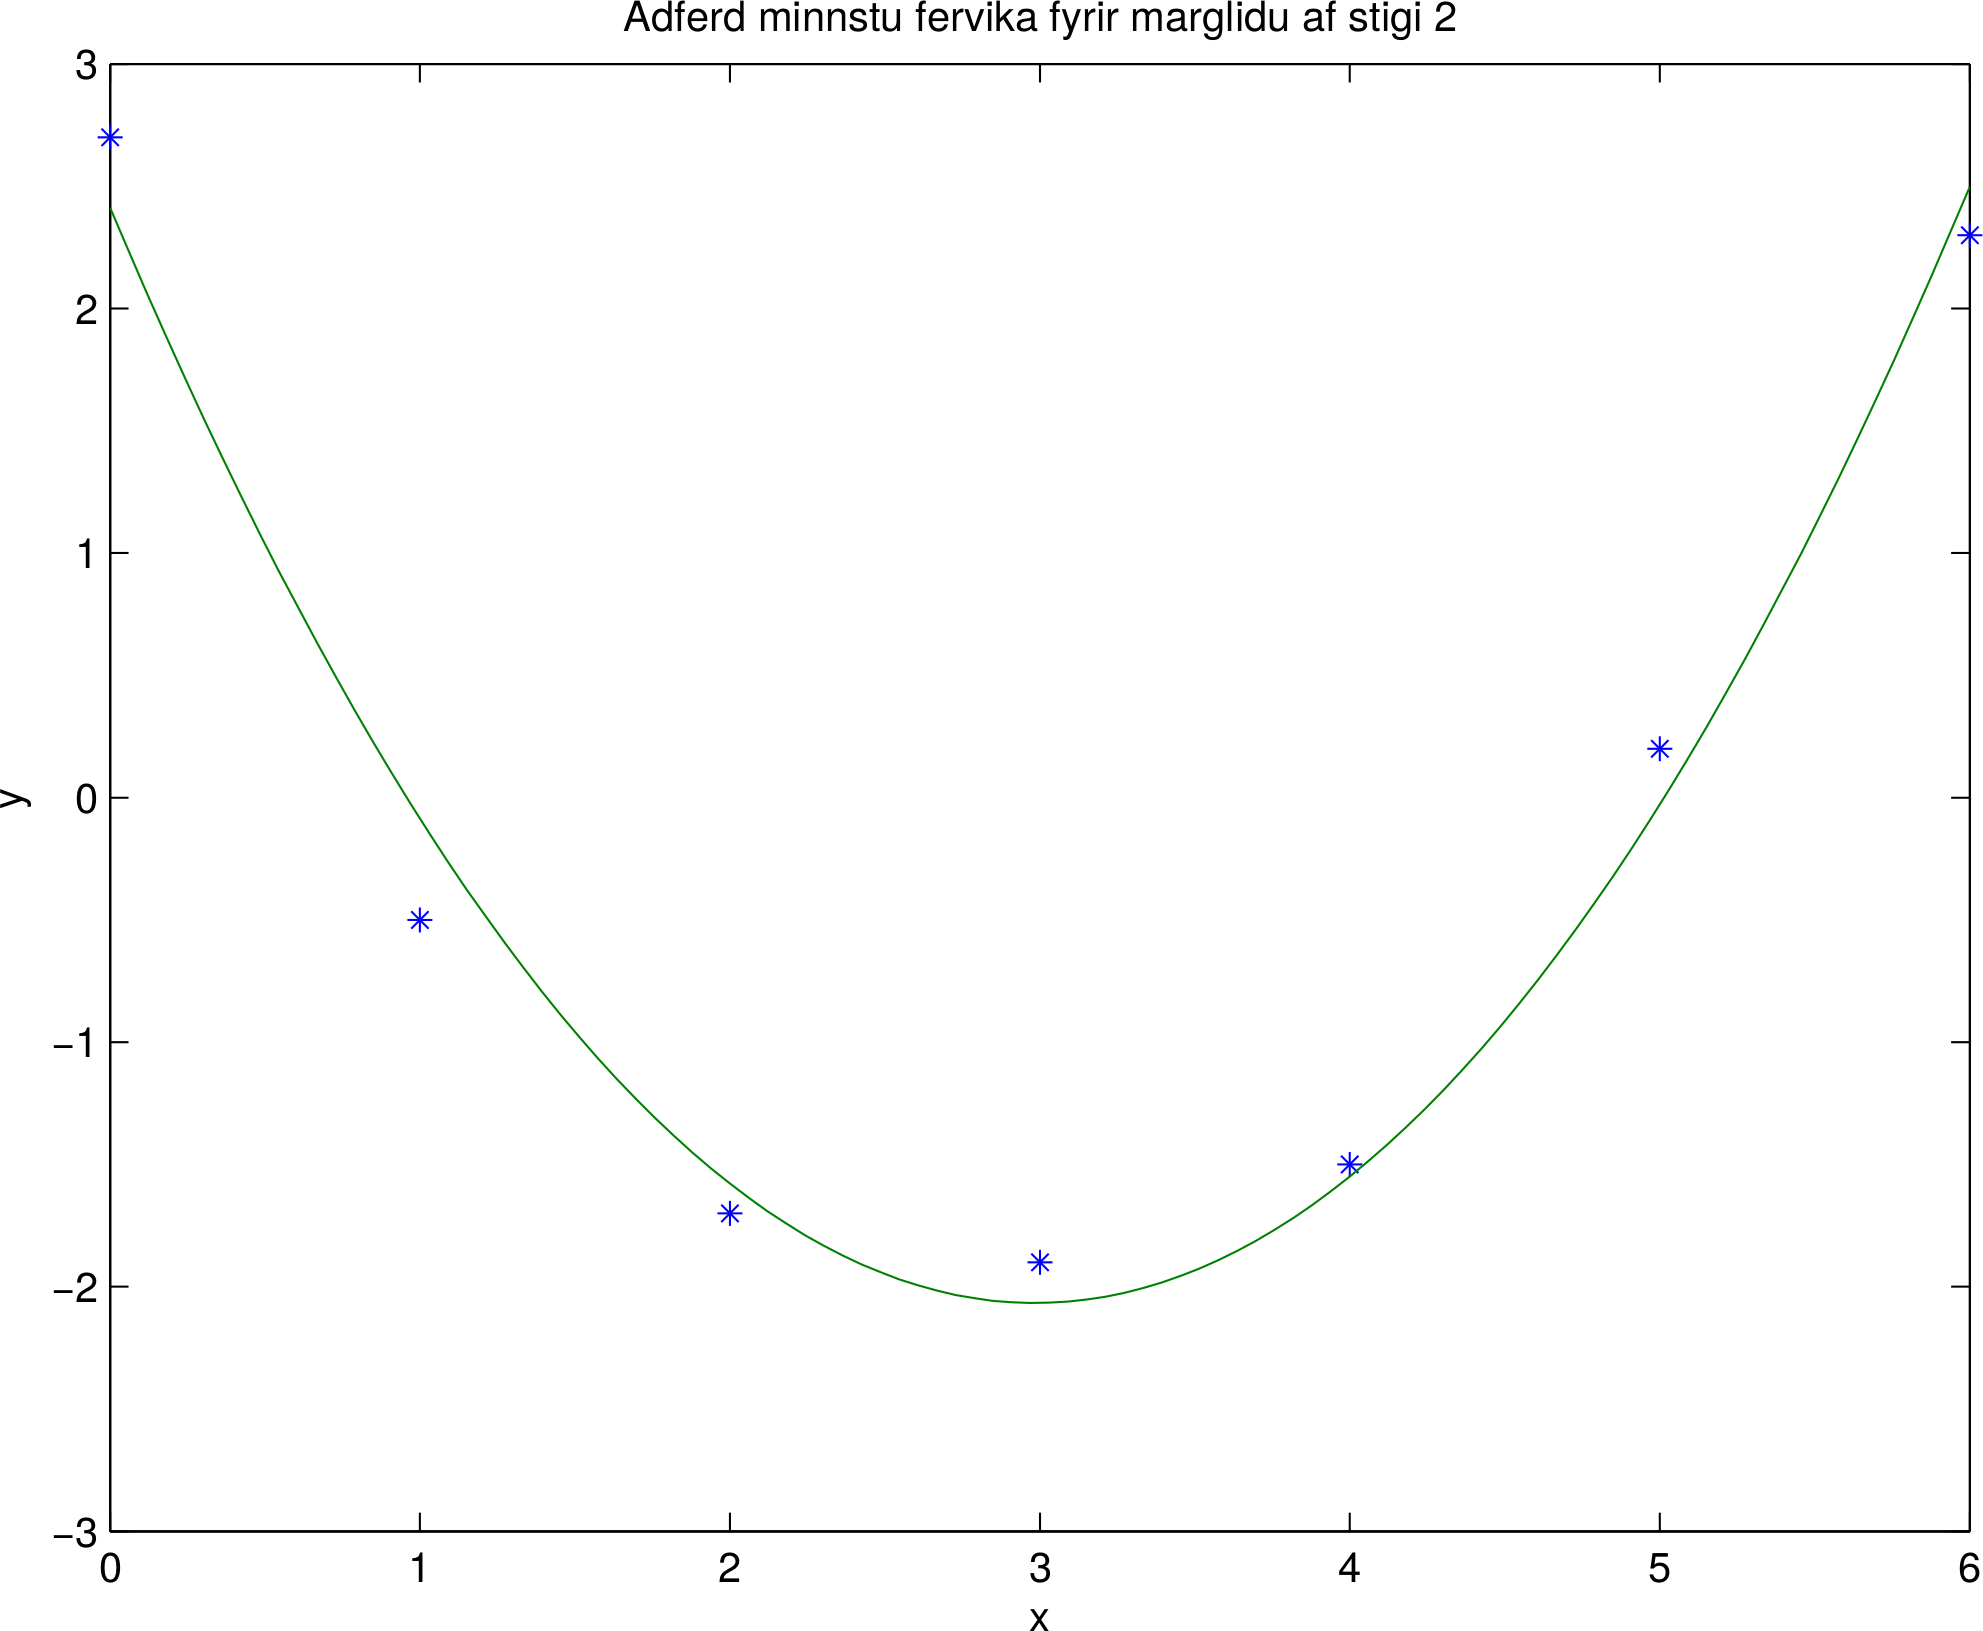
\includegraphics{synidaemi_minnstu_fervik.png}


\chapter{Töluleg diffrun}
\label{kafli04:toluleg-diffrun}\label{kafli04::doc}
\emph{Nanny's philosophy of life was to do what seemed like a good idea at the time, and do it as hard as possible. It had never let her down.}
-- Terry Pratchett, Maskerade


\section{Inngangur}
\label{kafli04:inngangur}
\index{töluleg diffrun}\index{töluleg heildun}

\subsection{Töluleg diffrun og heildun}
\label{kafli04:toluleg-diffrun-og-heildun}\label{kafli04:index-0}
Deildun og heildun eru meginaðgerðir stærðfræðigreiningarinnar.

Þess vegna er nauðsynlegt að geta nálgað
\begin{gather}
\begin{split}f'(a),f''(a),f'''(a),\dots \quad
  \text{ og } \quad
  \int_a^b f(x)\, dx,\end{split}\notag
\end{gather}
þar sem \(f\) er fall sem skilgreint er á bili \(I\) sem
inniheldur \(a\) og \(b\).


\subsection{Meginhugmynd í öllum nálgunaraðferðunum}
\label{kafli04:meginhugmynd-i-ollum-nalgunaraferunum}
Látum \(p\) vera margliðu sem nálgar \(f\), og látum
\(r(x)=f(x)-p(x)\) tákna skekkjuna í nálgun á \(f(x)\) með
\(p(x)\). Þá er
\begin{gather}
\begin{split}f'(x)=p'(x)+r'(x), \quad f''(x)=p''(x)+r''(x), \dots\end{split}\notag
\end{gather}
og
\begin{gather}
\begin{split}\int_a^b f(x)\, dx=\int_a^b p(x)\, dx+\int_a^b r(x)\, dx.\end{split}\notag
\end{gather}
Nú þurfum við að gera tvennt:
\begin{enumerate}
\item {} 
Finna heppilegar nálgunarmargliður og reikna út
\begin{gather}
\begin{split}p'(a), \ p''(a),\dots, \qquad \int_a^b p(x)\, dx\end{split}\notag
\end{gather}
\item {} 
Meta skekkjurnar
\begin{gather}
\begin{split}r'(a), \ r''(a), \dots \int_a^b r(x)\, dx\end{split}\notag
\end{gather}
\end{enumerate}

Byrjum á að leiða út nokkrar nálgunarformúlur með skekkjumati.

\index{afleiður}\index{töluleg diffrun!frammismunur}

\section{Aðferðirnar}
\label{kafli04:index-1}\label{kafli04:aferirnar}
Látum \(f : I \to \mathbb R\) vera fall á bili
\(I \subset \mathbb R\) og \(a\) vera punkt í \(I\). Afleiða
\(f\) í punktinum \(a\) er skilgreind með
\begin{gather}
\begin{split}f'(a) = \lim\limits_{h \to 0}
  \frac{f(a+h)-f(a)}{h}\end{split}\notag
\end{gather}
ef markgildið er til. Við skrifum því oft
\begin{gather}
\begin{split}f'(a) \approx \frac{f(a+h)-f(a)}{h}\end{split}\notag
\end{gather}
Þessi nálgun er kölluð \emph{frammismunur} því oftast hugsar maður sér að
\(h > 0\) og þá er \(a+h\) lítið skref áfram frá \(a\).

Við þurfum skekkjumat fyrir þessa formúlu ef við eigum að geta notað
hana.


\subsection{Frammismunur}
\label{kafli04:frammismunur}
Við fáum mat á skekkjuna í nálguninni með að skoða Taylor-margliðu
\(f\) í \(a\). Samkvæmt setningu Taylors er til \(\xi\) á
milli \(a\) og \(a+h\) þannig að
\begin{gather}
\begin{split}f(a+h) = f(a) + f'(a)h + \frac{1}{2} f''(\xi)h^2.\end{split}\notag
\end{gather}
Þá fæst að skekkjan í nálgun á \(f'(a)\) með
\begin{gather}
\begin{split}\frac{f(a+h)-f(a)}{h} = f[a,a+h]\end{split}\notag
\end{gather}
er
\begin{gather}
\begin{split}e = f'(a) - \frac{f(a+h)-f(a)}{h} = -\frac{1}{2} f''(\xi) h\end{split}\notag
\end{gather}
Með öðrum orðum
\begin{gather}
\begin{split}\min_{t\in [0,h]} -\frac 12 f''(t)h \leq e \leq
\max_{t\in [0,h]} -\frac 12 f''(t)h.\end{split}\notag
\end{gather}
Við sjáum því að \(e=O(h)\) þegar \(h \to 0\).

\index{töluleg diffrun!bakmismunur}

\subsection{Bakmismunur}
\label{kafli04:bakmismunur}\label{kafli04:index-2}
Við getum sett \(a-h\) í stað \(a+h\) í skilgreininguna á
afleiðu. Þá fæst svokallaður \emph{bakmismunur}
\begin{gather}
\begin{split}f'(a) \approx \frac{f(a)-f(a-h)}{h}\end{split}\notag
\end{gather}
og ljóst er að sama skekkjumat gengur fyrir þessa nálgun og fyrir nálgun
með frammismun.

\index{töluleg diffrun!miðsettur mismunakvóti}

\subsection{Miðsettur mismunakvóti}
\label{kafli04:misettur-mismunakvoti}\label{kafli04:index-3}
Lítum nú á þriðja stigs Taylor nálgun
\begin{gather}
\begin{split}\begin{aligned}
  f(a+h)&=f(a)+f'(a)h+\tfrac 12 f''(a)h^2+\tfrac 16 f'''(\alpha)h^3,\\
  f(a-h)&=f(a)-f'(a)h+\tfrac 12 f''(a)h^2-\tfrac 16 f'''(\beta)h^3,\end{aligned}\end{split}\notag
\end{gather}
þar sem \(\alpha\) er á milli \(a\) og \(a+h\) og
\(\beta\) er á milli \(a\) og \(a-h\).

Tökum nú mismuninn og fáum
\begin{gather}
\begin{split}f(a+h)-f(a-h)=f'(a)\cdot 2h+\tfrac 16\big(f'''(\alpha)+f'''(\beta)\big)h^3\end{split}\notag
\end{gather}
Ef \(f'''\) er samfellt fall, þá gefur milligildissetningin okkur að
til er \(\xi\) á milli \(\alpha\) og \(\beta\) þannig að
\(f'''(\xi)=\tfrac 12 (f'''(\alpha)+f'''(\beta))\)

Niðurstaðan verður
\begin{gather}
\begin{split}f'(a)=\dfrac{f(a+h)-f(a-h)}{2h}-\tfrac 16f'''(\xi)h^2.\end{split}\notag
\end{gather}
Þannig að skekkjan er
\begin{gather}
\begin{split}e = -\frac 16 f'''(\xi) h^2,\end{split}\notag
\end{gather}
og jafnframt er \(e = O(h^2)\) þegar \(h\to 0\).


\begin{center}
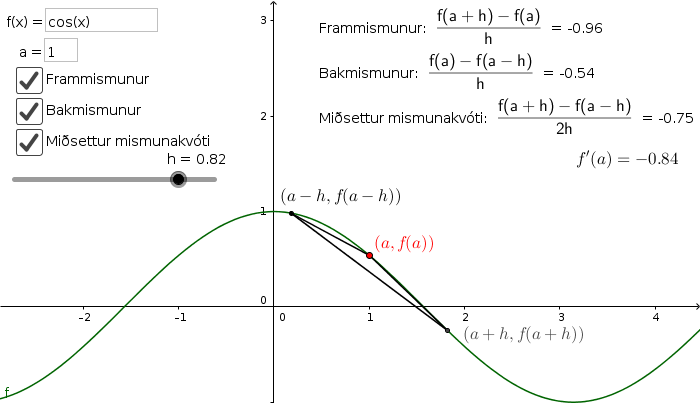
\includegraphics[width=12cm,keepaspectratio=true]{./afleida.png}
\end{center}


\index{töluleg diffrun!miðsetttur mismunakvóti fyrir aðra afleiðu}

\subsection{Miðsettur mismunakvóti fyrir aðra afleiðu}
\label{kafli04:misettur-mismunakvoti-fyrir-ara-afleiu}\label{kafli04:index-4}
Við getum útfært þessa sömu hugmynd til þess að reikna út aðra afleiðu,
en þá byrjum við með fjórða stigs Taylor-nálgun
\begin{gather}
\begin{split}\begin{aligned}
  f(a+h)&=f(a)+f'(a)h+\tfrac 12 f''(a)h^2+\tfrac 16 f'''(a)h^3
+\tfrac 1{24}f^{(4)}(\alpha)h^4,\\
  f(a-h)&=f(a)-f'(a)h+\tfrac 12 f''(a)h^2-\tfrac 16 f'''(a)h^3
+\tfrac 1{24}f^{(4)}(\beta)h^4,\end{aligned}\end{split}\notag
\end{gather}
þar sem \(\alpha\) er á milli \(a\) og \(a+h\) og
\(\beta\) er á milli \(a\) og \(a-h\).

Nú leggjum við saman og fáum
\begin{gather}
\begin{split}f(a+h)+f(a-h)=2f(a) +f''(a)h^2+\tfrac
1{24}\big(f^{(4)}(\alpha)+f^{(4)}(\beta)\big)h^4.\end{split}\notag
\end{gather}
Nú þurfum við að gefa okkur að \(f^{(4)}\) sé samfellt fall, þá
gefur milligildissetningin okkur að til er \(\xi\) á milli
\(\alpha\) og \(\beta\) þannig að
\(f^{(4)}(\xi)=\tfrac 12 (f^{(4)}(\alpha)+f^{(4)}(\beta))\).

Niðurstaðan verður
\begin{gather}
\begin{split}f''(a)=\dfrac{f(a+h)+f(a-h)-2f(a)}{h^2}-\tfrac 1{12}f^{(4)}(\xi)h^2\end{split}\notag
\end{gather}
Með Taylor-margliðum má leiða út fleiri nálgunarformúlur fyrir afleiður.

Við ætlum ekki að halda lengra í þessa átt heldur snúa okkur að almennu
aðferðinni.


\section{Skekkjumat}
\label{kafli04:skekkjumat}

\subsection{Almennt um nálganir á afleiðum}
\label{kafli04:almennt-um-nalganir-a-afleium}
Ef \(x_0,\ldots, x_n\) eru punktar í \(I\) (hugsanlega með
endurtekningum) og \(p\) er margliðan sem brúar \(f\) í þeim, þá
er
\begin{gather}
\begin{split}f(x) = p(x) + r(x),\end{split}\notag
\end{gather}
þar sem skekkjuliðurinn \(r(x)\) er gefinn með formúlunni
\begin{gather}
\begin{split}r(x)=f[x_0,\ldots,x_n,x](x-x_0)\cdots(x-x_n)\end{split}\notag
\end{gather}
Ef við tökum \(p'(a)\) sem nálgun á \(f'(a)\) er skekkjan
\begin{gather}
\begin{split}r'(a) =  f'(a) - p'(a).\end{split}\notag
\end{gather}
\index{töluleg diffrun!skekkjumat}

\subsection{Skekkjumat}
\label{kafli04:index-5}\label{kafli04:id1}
Munið að formúlan fyrir afleiðu af margfeldi margra þátta er
\begin{gather}
\begin{split}\begin{gathered}
  (\varphi_1\varphi_2\varphi_3\cdots\varphi_m)'(a)\\
=\varphi_1'(a)\varphi_2(a)\varphi_3(a)\cdots\varphi_m(a)
+\varphi_1(a)\varphi_2'(a)\varphi_3(a)\cdots\varphi_m(a)
+\cdots\\
\cdots+\varphi_1(a)\varphi_2(a)\cdots \varphi_{m-1}(a)\varphi_m'(a)\\\end{gathered}\end{split}\notag
\end{gather}
Horfum nú á skekkjuliðinn \(r(x)\). Hann er svona margfeldi með
\(\varphi_1(x)=f[x_0,\dots,x_n,x]\), \(\varphi_2(x)=x-x_0\),
\(\varphi_3(x)=x-x_1\) o.s.frv.

Athugum nú að ef \(a\) er einn af gefnu punktunum \(x_k\), þá er
\(\varphi_{k+2}(x)=(x-x_k)\) sem gefur \(\varphi_{k+2}(x_k)=0\)
og \(\varphi_{k+2}'(x_k)=1\).

Þetta segir okkur að ef við tökum \(a=x_k\), þá eru allir liðirnir í
summunni í hægri hliðinni \(0\) nema einn, þ.e. við sitjum eftir með
þann sem inniheldur \({\varphi}_{k+2}'\).

Niðurstaðan verður því að skekkjan í nálgun á \(f'(a)\) með
\(p'(a)\) er
\begin{gather}
\begin{split}\begin{aligned}
  f'(a) - p'(a) &= r'(a)
=f[x_0,\dots,x_n,x_k]
\prod_{\stackrel{j=0}{j \not= k}} (x_k-x_j)\\
&=\dfrac{f^{(n+1)}(\xi)}{(n+1)!}
  \prod_{\stackrel{j=0}{j \not= k}} (a-x_j)\end{aligned}\end{split}\notag
\end{gather}
þar sem \(a=x_k\).

Hér notuðum við skekkjumatið fyrir Newton aðferðina sem
segir að til er \(\xi\) á minnsta bilinu sem inniheldur
\(x_0,\ldots,x_n,x_k\) sem uppfyllir
\begin{gather}
\begin{split}f[x_0,\ldots,x_n,x_k] = \frac{f^{(n+1)}(\xi)}{(n+1)!}.\end{split}\notag
\end{gather}

\subsection{Frammismunur}
\label{kafli04:id2}
Nálgum \(f\) með fyrsta stigs brúunarmargliðunni gegnum punktana
\((a,f(a))\) og \((a+h,f(a+h))\) (þ.e. \(x_0 = a\) og
\(x_1 = a+h\)),
\begin{gather}
\begin{split}f(x)=f[a]+f[a,a+h](x-a)+f[a,a+h,x](x-a)(x-a-h)\end{split}\notag
\end{gather}
Af þessu leiðir formúlan sem við vorum áður komin með
\begin{gather}
\begin{split}f'(a)=f[a,a+h]+f[a,a+h,a](a-a-h)
  =\dfrac{f(a+h)-f(a)}h-\tfrac 12 f''(\xi)h\end{split}\notag
\end{gather}
Þar sem \(\xi\) er á milli \(a\) og \(a+h\) og uppfyllir að
\(f[a,a+h,a]=f[a,a,a+h]=\tfrac 12f''(\xi)\). Hér erum við að
notafæra okkur aftur skekkjumatið sem við sönnuðum í kaflanum um
brúunarmargliður.


\subsection{Miðsettur mismunakvóti}
\label{kafli04:id3}
Tökum þriggja punkta brúunarformúlu með \(a-h\), \(a+h\) og
\(a\). Þá er
\begin{gather}
\begin{split}\begin{aligned}
  f(x)&=f[a-h]+f[a-h,a+h](x-a+h)\\
  &+f[a-h,a+h,a](x-a+h)(x-a-h)\\
  &+f[a-h,a+h,a,x](x-a+h)(x-a-h)(x-a)\end{aligned}\end{split}\notag
\end{gather}
Athugum að afleiðan af annars stigs þættinum
\begin{gather}
\begin{split}x\mapsto (x-a+h)(x-a-h)=(x-a)^2-h^2\end{split}\notag
\end{gather}
er \(0\) í punktinum \(a\) og því er
\begin{gather}
\begin{split}\begin{aligned}
  f'(a)&=f[a-h,a+h]+f[a-h,a+h,a,a](-h^2)\\
  &=\dfrac{f(a+h)-f(a-h)}{2h}-\tfrac 16 f'''(\xi)h^2 \end{aligned}\end{split}\notag
\end{gather}
Hér nýttum við okkur að til er \(\xi\) á milli \(a-h\) og
\(a+h\) þannig að \(f[a-h,a+h,a,a]=\tfrac 16 f'''(\xi)\).


\subsection{Miðsettur mismunakvóti fyrir aðra afleiðu}
\label{kafli04:id4}
Áfram heldur leikurinn. Nú skulum við leiða aftur út formúluna fyrir
nálgun á \(f''(a)\) með miðsettum mismunakvóta

Þá tökum við þriggja punkta brúunarformúlu með \(a-h\), \(a+h\)
og \(a\) með \(a\) tvöfaldan. Þá er
\begin{gather}
\begin{split}\begin{aligned}
  f(x)&=f[a-h]+f[a-h,a+h](x-a+h)\\
  &+f[a-h,a+h,a](x-a+h)(x-a-h)\\
  &+f[a-h,a+h,a,a](x-a+h)(x-a-h)(x-a)\\
  &+f[a-h,a+h,a,a,x](x-a+h)(x-a-h)(x-a)^2\end{aligned}\end{split}\notag
\end{gather}
Gætum þess að halda liðnum \((x-a)\). Þá fáum við
\begin{gather}
\begin{split}\begin{aligned}
  f(x)&=f[a-h]+f[a-h,a+h](x-a+h)\\
  &+f[a-h,a+h,a]\big((x-a)^2-h^2)\big)\\
  &+f[a-h,a+h,a,a]\big((x-a)^3-h^2(x-a))\big)\\
  &+f[a-h,a+h,a,a,x]\big((x-a)^4-h^2(x-a)^2)\big)\end{aligned}\end{split}\notag
\end{gather}
Nú þurfum við að reikna aðra afleiðu í punktinum \(a\). Athugum að
önnur afleiða af annars stigs þættinum
\begin{gather}
\begin{split}x\mapsto (x-a+h)(x-a-h)=(x-a)^2-h^2\end{split}\notag
\end{gather}
er fastafallið \(2\), önnur afleiða af þriðja stigs liðnum
\begin{gather}
\begin{split}x\mapsto (x-a)^3-h^2(x-a)\end{split}\notag
\end{gather}
er \(0\) í punktinum \(a\) og önnur afleiða af fjórða stigs
liðnum
\begin{gather}
\begin{split}x\mapsto (x-a)^4-h^2(x-a)^2\end{split}\notag
\end{gather}
er fastafallið \(-2h^2\).

Við höfum því
\begin{gather}
\begin{split}f''(a)=2f[a-h,a+h,a]+f[a-h,a+h,a,a,a](-2h^2)\end{split}\notag
\end{gather}
Nú er til punktur \(\xi\) á minnsta bili sem inniheldur \(a-h\),
\(a+h\) og \(a\) þannig að \(f[a-h,a+h,a,a,a]=\tfrac
1{24}f^{(4)}(\xi)\).

Við þurfum að reikna út fyrri mismunakvótann
\begin{gather}
\begin{split}\begin{aligned}
  f[a-h,a+h,a]&=f[a-h,a,a+h]=\dfrac{f[a,a+h]-f[a-h,a]}{2h}\\
  &=\dfrac 1{2h}\bigg(\dfrac{f(a+h)-f(a)}h-\dfrac{f(a)-f(a-h)}h\bigg)\\
  &=\dfrac{f(a+h)+f(a-h)-2f(a)}{2h^2}  \end{aligned}\end{split}\notag
\end{gather}
Við höfum því leitt aftur út formúluna
\begin{gather}
\begin{split}f''(a)=\dfrac{f(a+h)+f(a-h)-2f(a)}{h^2}-\tfrac
  1{12}f^{(4)}(\xi)h^2\end{split}\notag
\end{gather}
\index{töluleg diffrun!Richardson útgiskun}

\section{Richardson útgiskun}
\label{kafli04:index-6}\label{kafli04:richardson-utgiskun}
Það ætti að vera ljóst að töluleg deildun er nokkuð óstöðug aðferð því
ef skrefastærðin \(h\) er lítil eru tölurnar
\(f(a+h), f(a), f(a-h)\) nálægt hver annarri og við getum lent í
styttingarskekkjum.

Því er ekki hægt að búast við að fá alltaf betri nálgun á \(f'(a)\)
við að minnka skrefalengdina \(h\).

Leiðin er Richardson útgiskun (e. extrapolation), sem er aðferð til að
bæta nálganir.

Til eru mjög almennar útgáfur þessarar aðferðar en við munum aðeins
skoða þau sértilfelli sem nýtast okkur mest.


\subsection{Útleiðsla á miðsettum mismunakvóta}
\label{kafli04:utleisla-a-misettum-mismunakvota}
Við skulum byrja á að að leiða aftur út formúluna fyrir miðsettann
mismunakvóta til að fá betri upplýsingar um skekkjuliðinn. Fyrir fall
\(f\) sem er nógu oft deildanlegt má beita Taylor til að skrifa
\begin{gather}
\begin{split}\begin{aligned}
  f(a+h) &= f(a) + f'(a)h   + \ldots
  + \frac{f^{(2n)}(a)}{(2n!)}h^{2n}
  + \frac{f^{(2n+1)}(a)}{(2n+1)!)}h^{2n+1} + O(h^{2n+2}) \\
  f(a-h) &= f(a) - f'(a)h
    + \ldots
  + \frac{f^{(2n)}(a)}{(2n!)}h^{2n}
  - \frac{f^{(2n+1)}(a)}{(2n+1)!)}h^{2n+1} + O(h^{2n+2})\end{aligned}\end{split}\notag
\end{gather}
Ef við drögum seinni jöfnuna frá þeirri fyrri fæst
\begin{gather}
\begin{split}f(a+h)-f(a-h) = 2f'(a)h + 2\frac{f'''(a)}{3!}h^3
  + \ldots + 2\frac{f^{(2n+1)}(a)}{(2n+1)!}h^{2n+1} + O(h^{2n+2})\end{split}\notag
\end{gather}
svo ef við einangrum \(f'(a)\) sjáum við að
\begin{gather}
\begin{split}f'(a) = R_1(h)
  + a_2 h^2 + a_4 h^4 + \ldots + a_{2n} h^{2n} + O(h^{2n+1})\end{split}\notag
\end{gather}
þar sem
\begin{gather}
\begin{split}R_1(h) = \frac{f(a+h)-f(a-h)}{2h}
  \quad \text{og} \quad
  a_k = -\frac{f^{(k+1)}(a)}{(k+1)!},
  \quad k = 2,4,\ldots,2n.\end{split}\notag
\end{gather}

\subsection{Helmingun á skrefinu}
\label{kafli04:helmingun-a-skrefinu}
Hér er minnsta veldi í skekkjuliðnum \(h^2\), svo nálgunin
\(f'(a)
\approx R_1(h)\) er \(O(h^2)\), eins og við höfum reyndar séð áður.
Helmingum nú skrefalengdina \(h\), þá fæst
\begin{gather}
\begin{split}f'(a) = R_1(h/2) + a_2 \left(\frac{h}{2}\right)^2
  + a_4 \left(\frac{h}{2}\right)^4 + \ldots
  + a_{2n} \left(\frac{h}{2}\right)^{2n} + O(h^{2n+1}).\end{split}\notag
\end{gather}
Nú berum við saman þessi tvö skref:
\begin{gather}
\begin{split}\begin{aligned}
  f'(a) &= R_1(h/2) + \tfrac 14 a_2 h^2
  + a_4 \left(\frac{h}{2}\right)^4 + \ldots
  + a_{2n} \left(\frac{h}{2}\right)^{2n} + O(h^{2n+1}),\\
  f'(a) &= R_1(h)
  + a_2 h^2 + a_4 h^4 + \ldots + a_{2n} h^{2n} + O(h^{2n+1})\\\end{aligned}\end{split}\notag
\end{gather}
Margföldum efri jöfnuna með \(4\) og drögum þá síðari frá. Þá
stendur eftir
\begin{gather}
\begin{split}\begin{aligned}
  3f'(a) &= 4 R_1(h/2) - R_1(h)
  + a_4 \left( \frac{4}{2^4} - 1 \right)h^4 \\
  &+ a_6 \left( \frac{4}{2^6} - 1 \right)h^6
  + \ldots
  + a_{2n} \left( \frac{4}{2^{2n}} - 1 \right)h^{2n}
  + O(h^{2n+1})\end{aligned}\end{split}\notag
\end{gather}

\subsection{Fjórða stigs nálgun}
\label{kafli04:fjora-stigs-nalgun}
Nú erum við komin með nýja formúlu:
\begin{gather}
\begin{split}f'(a) = R_2(h) + b_4 h^4 + b_6 h^6 + \ldots + b_{2n} h^{2n}
  + O(h^{2n+1})\end{split}\notag
\end{gather}
þar sem
\begin{gather}
\begin{split}R_2(h) = \frac{4 R_1(h/2) - R_1(h)}{3}
  \quad \text{og} \quad
  b_k = \frac{a_k}{3} \cdot \left(\frac{4}{2^k}-1\right),
  \  k = 4,6,\ldots,2n.\end{split}\notag
\end{gather}
Ef við berum þetta saman við jöfnuna sem við byrjuðum með
\begin{gather}
\begin{split}f'(a) = R_1(h)
  + a_2 h^2 + a_4 h^4 + \ldots + a_{2n} h^{2n} + O(h^{2n+1})\end{split}\notag
\end{gather}
þá sjáum við að minnsta veldi í skekkjuliðnum er \(h^4\), svo
nálgunin \(f'(a)
\approx R_2(h)\) uppfyllir
\begin{gather}
\begin{split}f'(a) - R_2(h) = O(h^4)\end{split}\notag
\end{gather}
og er því betri nálgun en áður.

Þetta ferli heitir \emph{Richardson útgiskun}.


\subsection{Hægt er að halda áfram útgiskun}
\label{kafli04:haegt-er-a-halda-afram-utgiskun}
Næsta takmark er að eyða liðnum \(b_4h^4\) úr þessari formúlu með
því að líta á
\begin{gather}
\begin{split}f'(a) = R_2(h/2) + b_4 \left(\frac{h}{2}\right)^4
  + b_6 \left(\frac{h}{2}\right)^6 + \ldots
  + b_{2n} \left(\frac{h}{2}\right)^{2n} + O(h^{2n+1})\end{split}\notag
\end{gather}
Síðan stillum við þessari jöfnu upp með þeirri síðari
\begin{gather}
\begin{split}\begin{aligned}
  f'(a) &= R_2(h/2) + \tfrac 1{16}b_4 h^4
  + \tfrac 1{64}b_6 h^6 + \ldots
  + \tfrac 1{2^{2n}}b_{2n} h^{2n} + O(h^{2n+1})\\
  f'(a) &= R_2(h) + b_4 h^4 + b_6 h^6 + \ldots + b_{2n} h^{2n}
  + O(h^{2n+1})\end{aligned}\end{split}\notag
\end{gather}
Margföldum fyrri jöfnuna með \(16\) og drögum þá síðari frá
\begin{gather}
\begin{split}\begin{aligned}
  15f'(a) &= 16 R_2(h/2) - R_2(h)
  + b_6 \left( \frac{16}{2^6} - 1 \right) h^6 \\
  &+ b_8 \left( \frac{16}{2^8} - 1 \right) h^8
  + \ldots
  + b_{2n} \left( \frac{16}{2^{2n}} - 1 \right) h^{2n}
  + O(h^{2n+1}).\end{aligned}\end{split}\notag
\end{gather}

\subsection{Sjötta stigs skekkja}
\label{kafli04:sjotta-stigs-skekkja}\begin{gather}
\begin{split}\begin{aligned}
  15f'(a) &= 16 R_2(h/2) - R_2(h)
  + b_6 \left( \frac{16}{2^6} - 1 \right) h^6 \\
  &+ b_8 \left( \frac{16}{2^8} - 1 \right) h^8
  + \ldots
  + b_{2n} \left( \frac{16}{2^{2n}} - 1 \right) h^{2n}
  + O(h^{2n+1}).\end{aligned}\end{split}\notag
\end{gather}
Því er
\begin{gather}
\begin{split}f'(a) = R_3(h) + c_6 h^6 + c_8 h^8 \ldots + c_{2n} h^{2n}
  + O(h^{2n+1})\end{split}\notag
\end{gather}
þar sem
\begin{gather}
\begin{split}R_3(h) = \frac{16 R_2(h/2) - R_2(h)}{15},
  \quad \text{og} \quad
  c_k = \frac{b_k}{15} \cdot \left( \frac{16}{2^k} - 1 \right),
  \quad k = 6,8,\ldots,2n.\end{split}\notag
\end{gather}
Nýja nálgunin uppfyllir
\begin{gather}
\begin{split}f'(a) - R_3(h) = O(h^6)\end{split}\notag
\end{gather}
og er því enn betri en áður, en við þurfum líka að reikna út
\(R_1(h/4)\) til að reikna \(R_2(h/2)\).


\subsection{Almenn rakningarformúla}
\label{kafli04:almenn-rakningarformula}
Richardson-útgiskunin heldur áfram og út kemur
\begin{gather}
\begin{split}R_{i+1}(h) = \frac{4^i R_i(h/2) - R_i(h)}{4^i-1}
  = R_i(h/2) + \frac{R_i(h/2)-R_i(h)}{4^i-1}\end{split}\notag
\end{gather}
fyrir \((i+1)\)-tu Richardson útgiskun og \(R_{i+1}(h)\)
uppfyllir að
\begin{gather}
\begin{split}f'(a) - R_{i+1}(h) = O(h^{2i+2}),\end{split}\notag
\end{gather}
en á móti kemur að til að reikna út \(R_{i+1}(h)\) þurfum við að
hafa reiknað út tölurnar

\begin{DUlineblock}{0em}
\item[] \(R_1(h)\), \(R_1(h/2)\), \(\ldots\), \(R_1(h/2^i)\)
auk
\item[] \(R_2(h)\), \(R_2(h/2)\), …, \(R_2(h/2^{i-1})\) og svo
framvegis að
\item[] \(\qquad \vdots\)
\item[] \(R_i(h)\) og \(R_i(h/2)\).
\end{DUlineblock}

Eins og áður sagði fara styttingarskekkjur á endanum að segja til sín í
útreikningum á \(R_1(h)\), svo einhver takmörk eru fyrir hversu
margar Richardson útgiskanir er hægt að framkvæma.


\subsection{Reiknirit}
\label{kafli04:reiknirit}
Útreikningarnir að ofan eru yfirleitt settir fram í töflu
\begin{gather}
\begin{split}\begin{array}{ccccc}
    D(1,1) &   &   &   &   \\
    D(2,1) & D(2,2) &  &  &  \\
    D(3,1) & D(3,2) & D(3,3) & & \\
    \vdots & \vdots & \vdots & \ddots & \\
    D(n,1) & D(n,2) & D(n,3) & \ldots & D(n,n)
  \end{array}\end{split}\notag
\end{gather}
þar sem \(D(i,j) = R_j(h/2^{i-j})\) og þar með
\begin{gather}
\begin{split}D(i,j) = \begin{cases}
    \dfrac{f(a+h/2^{i-1})-f(a-h/2^{i-1})}{2\cdot h/2^{i-1}}, & j = 1 \\
    D(i,j-1) + \dfrac{D(i,j-1)-D(i-1,j-1)}{4^{j-1}-1}, & j > 1
  \end{cases}\end{split}\notag
\end{gather}
sem gerir okkur auðvelt að forrita Richardson útgiskun.


\subsection{Skekkjumat}
\label{kafli04:id5}
Finnum nú eftirámat fyrir \(D(i,j)\) með stærðunum
\(D(i,j-1)\) og \(D(i-1,j-1)\). Hér á eftir er
\(R_j(h/2)\) í hlutverki \(D(i,j-1)\) og \(R_i(h)\) í
hlutverki \(D(i-1,j-1)\)
(\(h\) er helmingað þegar við förum niður um eina línu).

Munum að \(R_i(h)\) uppfyllir að
\begin{gather}
\begin{split}f'(a) = R_j(h) + Kh^{2j} + O(h^{2j+1})\end{split}\notag
\end{gather}
fyrir eitthvert \(K\) í \(\mathbb R\) og að
\begin{gather}
\begin{split}f'(a) = R_j(h/2) + K \left( \frac{h}{2} \right)^{2j}
  + O(h^{2j+1})\end{split}\notag
\end{gather}
Ef við tökum mismun á hægri og vinstri hliðum þessara jafna, þá fáum við
\begin{gather}
\begin{split}0 = R_j(h) - R_j(h/2) + K \left(1 - \frac{1}{2^{2j}}\right)h^{2j}
  + O(h^{2j+1})\end{split}\notag
\end{gather}
og ef við einangrum \(K\) fæst
\begin{gather}
\begin{split}K = -\frac{4^{j}}{h^{2j}} \cdot \frac{R_j(h)-R_j(h/2)}{4^{j}-1} +
O(h^{2j+1}).\end{split}\notag
\end{gather}

\subsection{Útleiðsla á fyrirframmati}
\label{kafli04:utleisla-a-fyrirframmati}
Þá er skekkjan í nálgun á \(f'(a)\) með \(R_j(h/2)\) jöfn
\begin{gather}
\begin{split}\begin{aligned}
  e_j(h/2) &= f'(a) - R_j(h/2) \\
  &= K\left(\frac{h}{2}\right)^{2j} + O(h^{2j+1}) \\
  &= -\frac{R_j(h)-R_j(h/2)}{4^{j}-1} + O(h^{2j+1}) \\
  &\approx -\frac{R_j(h)-R_j(h/2)}{4^{j}-1}.\end{aligned}\end{split}\notag
\end{gather}
Þar sem \(R_j(h/2)\) er nálgun á \(f'(a)\) af stigi
\(O(h^{2j+1})\), en \(R_{j+1}(h)\) er nálgun á \(f'(a)\) af
stigi \(O(h^{2i+3})\) getum við slegið á \(e_{j+1}(h)\) með
\(e_j(h/2)\). Ef við lækkum vísinn \(j+1\) um einn gefur það
okkur matið
\begin{gather}
\begin{split}e_j(h) \approx \frac{R_{j-1}(h)-R_{j-1}(h/2)}{4^{j-1}-1} =
  \frac{D(i,j-1)-D(i-1,j-1)}{4^{j-1}-1}\end{split}\notag
\end{gather}
sem er einmitt liðurinn í rakningarformúlunni fyrir \(D(i,j)\).


\subsection{Sýnidæmi}
\label{kafli04:synidaemi}
Látum \(f(x)=x/(x^2+4)^{2/3}\) og \(a=-1\). Byrjum með
\(h=1\) og notum svo rakningarformúluna til þess að fylla út
útgiskunartöfluna.

\begin{tabulary}{\linewidth}{|L|L|L|L|L|}
\hline
\textsf{\relax 
\(h\)
} & \textsf{\relax 
\(D(i,1)\)
} & \textsf{\relax 
\(D(i,2)\)
} & \textsf{\relax 
\(D(i,3)\)
} & \textsf{\relax 
\(D(i,4)\)
}\\
\hline
1 .
 & 
0.25000000
 &  &  & \\
\hline
0.5
 & 
0.25151838
 & 
0.25202451
 &  & \\
\hline
0.25
 & 
0.25104655
 & 
0.25088928
 & 
0.25081360
 & \\
\hline
0.125
 & 
0.25086355
 & 
0.25080254
 & 
0.25079676
 & 
0.25079649
\\
\hline\end{tabulary}


Niðustaðan er: \(f'(-1)\approx   0.2507964\), með eftirámat á
skekkju \(-3\cdot 10^{-7}\).

Rétt gildi er \(0.25079647217924889177\).

% 
 \chapter{Töluleg heildun}
% \label{kafli05:toluleg-heildun}\label{kafli05:heildun}\label{kafli05::doc}
 \textbf{Í VINNSLU}
% 
% Gerum ráð fyrir að \(x_0,x_1, \ldots, x_n\) séu punktar á bilinu
% \([a,b]\) og að við þekkjum gildi \(f\) í þessum punktum. Þá
% getum við fundið brúunarmargliðuna \(p_n\) gegnum punktana
% \((x_k,f(x_k))\) og skrifað
% \begin{gather}
% \begin{split}f(x) = p_n(x) + r_n(x),\end{split}\notag
% \end{gather}
% þar sem leifin \(r_n\) er gefin með
% \begin{gather}
% \begin{split}r_n(x) = f[x_0,\ldots,x_n,x](x-x_0)\cdots(x-x_n).\end{split}\notag\\\begin{split}Nú er auðvelt að reikna heildi margliða, svo við nálgum heildi\end{split}\notag
% \end{gather}
% \(f\) með
% \begin{gather}
% \begin{split}  \int\limits_a^b f(x) dx \approx
%     I_n(f) := \int\limits_a^b p_n(x) dx\end{split}\notag\\\begin{split}og skekkjan í þessari nálgun er gefin með\end{split}\notag
% \end{gather}\begin{gather}
% \begin{split}e_n = \int\limits_a^b r_n(x) dx.\end{split}\notag\\\begin{split}Þessi aðferð er kölluð *Newton-Cotes-heildun*.\end{split}\notag
% \end{gather}
% 
% \section{Newton-Cotes -heildun}
% \label{kafli05:newton-cotes-heildun}
% Hugsum okkur að brúunarpunktarnir \(x_0, \ldots, x_n\) séu ólíkir.
% Þá getum við skrifað \(p_n\) með Lagrange-margliðum
% \begin{gather}
% \begin{split}p_n(x) = \sum\limits_{k=0}^n f(x_k) \ell_k(x),
%   \quad
%   \ell_k(x) = \prod\limits_{\stackrel{j=0}{j \not= k}}^n
%   \frac{(x-x_j)}{(x_k-x_j)},\end{split}\notag
% \end{gather}
% og þá er heildi \(p_n\) jafnt
% \begin{gather}
% \begin{split}\int\limits_a^b p_n(x) dx =
%   \sum\limits_{k=0}^n f(x_k) A_k,
%   \quad \text{þar sem} \quad
%   A_k = \int\limits_a^b \ell_k(x) dx.\end{split}\notag
% \end{gather}
% Athugið að gildi \(A_k\) veltur aðeins á brúunarpunktunum
% \(x_0, \ldots,
% x_n\) en ekki gildum \(f(x_k)\). Ef það á að heilda mörg föll yfir
% sama bil er því hægt að reikna gildi \(A_k\) í eitt skipti fyrir öll
% og endurnýta þau svo.
% 
% 
% \section{Sýnidæmi}
% \label{kafli05:synidaemi}
% Metum heildi \(f(x) = e^{-x}\cos(x)\) og
% \(g(x) = \sin (\frac{x^2}{2})\) yfir bilið \([0,2]\) með að nota
% skiptipunktana \(x_0 = 0\), \(x_1 = 1\) og \(x_2 = 2\).
% Lagrange-margliðurnar sem við eiga eru
% \begin{gather}
% \begin{split}\ell_0(x) = \frac{(x-1)(x-2)}{2}, \quad
%   \ell_1(x) = -x(x-2), \quad
%   \ell_2(x) = \frac{x(x-1)}{2}\end{split}\notag
% \end{gather}
% svo við fáum að
% \begin{gather}
% \begin{split}\begin{gathered}
%   A_0 = \frac{1}{2} \int\limits_0^2 (x-1)(x-2) dx = \frac{1}{3},
%   \qquad
%   A_1 = -\int\limits_0^2 x(x-2) dx = \frac{4}{3}, \\
%   A_2 = \frac{1}{2} \int\limits_0^2 x(x-1) dx = \frac{1}{3}.\end{gathered}\end{split}\notag
% \end{gather}
% Nú eru stuðlarnir fundnir og því fáum við
% \begin{gather}
% \begin{split}\begin{aligned}
%   \int\limits_0^2 f(x) dx &\approx
%   f(0)\frac{1}{3} + f(1)\frac{4}{3} + f(2)\frac{1}{3}\\
%   &= \frac{1 + 4e^{-1}\cos(1) + e^{-2}\cos(2)}{3}
%   \approx 0.59581\end{aligned}\end{split}\notag
% \end{gather}
% og
% \begin{gather}
% \begin{split}\begin{aligned}
%   \int\limits_0^2 g(x) dx &\approx
%   g(0)\frac{1}{3} + g(1)\frac{4}{3} + g(2)\frac{1}{3}\\
%  & = \frac{4\sin(1/2) + \sin(2)}{3}
%   \approx 0.91972.\end{aligned}\end{split}\notag
% \end{gather}
% Gildi heildanna eru \(\int\limits_0^2 f(x) dx \approx 0.58969\) og
% \(\int\limits_0^2 g(x) dx \approx 0.99762\) með 5 réttum aukastöfum
% svo nálgunargildin verða að teljast nokkuð góð miðað við hversu lítið
% fór í þau.
% 
% 
% \section{Trapisuregla}
% \label{kafli05:trapisuregla}
% Nú ætlum við að leiða út formúlur fyrir helstu reglum fyrir nálgun á
% heildum. Sú fyrsta er \emph{trapisuregla}.
% 
% Veljum \(x_0 = a\) og \(x_1 = b\) sem skiptipunktana okkar. Þá
% er graf \(p_1\) línustrikið gegnum \((a,f(a))\) og
% \((b,f(b))\),
% \begin{gather}
% \begin{split}p_1(x) = f(a) \ell_0(x) + f(b) \ell_1(x)
%   = f(a)\frac{b-x}{b-a} + f(b) \frac{x-a}{b-a}\end{split}\notag
% \end{gather}
% og vigtirnar eru
% \begin{gather}
% \begin{split}A_0 = \int\limits_a^b \ell_0(x) = \frac{b-a}{2} = A_1,\end{split}\notag\\\begin{split}svo\end{split}\notag
% \end{gather}\begin{gather}
% \begin{split}  \int\limits_a^b f(x) dx \approx
%     \frac{b-a}{2}\left(f(a)+f(b)\right).\end{split}\notag\\\begin{split}Trapisureglan er kölluð þessu nafni því með henni nálgum við heildi\end{split}\notag
% \end{gather}
% \(f\) með flatarmáli trapisunnar sem hefur hornpunktana
% \((a,0)\), \((b,0)\), \((b,f(b))\) og \((a,f(a))\).
% 
% 
% \section{Miðpunktsregla}
% \label{kafli05:mipunktsregla}
% Enn einfaldari er miðpunktsreglan, þá veljum við aðeins einn
% skiptipunkt, \(x_0 = \frac{1}{2}(a+b)\), og brúunarmargliðan verður
% fastamargliðan \(p_0(x) = f(x_0)\). Þá er
% \begin{gather}
% \begin{split}\int\limits_a^b f(x) dx \approx (b-a)f\left(\frac{a+b}{2}\right)\end{split}\notag
% \end{gather}
% 
% \section{Regla Simpsons}
% \label{kafli05:regla-simpsons}
% Nú veljum við þrjá skiptipunkta, \(x_0 = a\), \(x_1 = b\) og
% \(x_2 =
% \frac{1}{2}(a+b)\). Til einföldunar skulum við hliðra fallinu \(f\)
% um miðpunkt bilsins \(m=\tfrac{1}{2}(a+b)\).
% 
% Við skilgreinum \(\alpha=\tfrac 12(b-a)\) og
% \(g(x) = f\big(x+m\big)\)
% 
% Þá hliðrast \(a\), \(m\) og \(b\) yfir í \(-\alpha\),
% \(0\) og \(\alpha\) og
% \begin{gather}
% \begin{split}\int\limits_{-\alpha}^{\alpha} g(x) dx =
%   \int\limits_a^b f(x) dx.\end{split}\notag
% \end{gather}
% Lagrange margliðurnar og vigtirnar eru
% \begin{gather}
% \begin{split}\begin{aligned}
%   l_0(x) &= \frac{(x-\alpha)x}{(-\alpha-\alpha)(-\alpha - 0)}
%   = \frac{(x-\alpha)x}{2\alpha^2} \\
%   A_0 &= \int_{-\alpha}^{\alpha} l_0(x)\,dx = \frac{\alpha}{3} \\
%   l_1(x) &= \frac{(x-(-\alpha))(x-0)}{(\alpha - ( -\alpha))(\alpha - 0)}
%   = \frac{(x+\alpha)x}{2\alpha^2}\\
%   A_1 &= \int_{-\alpha}^{\alpha} l_1(x)\,dx = \frac{\alpha}{3}\\
%   l_2(x) &= \frac{(x-(\alpha))(x-\alpha)}{0-(-\alpha)(0-\alpha)}
%   = \frac{(x+\alpha)(x-\alpha)}{-\alpha^2}\\
%   A_2 &= \int_{\alpha}^{\alpha} l_2(x)\,dx = \frac{4\alpha}{3}\end{aligned}\end{split}\notag
% \end{gather}
% Nálgunarformúlan verður þá
% \begin{gather}
% \begin{split}\begin{aligned}
%   \int_a^b f(x) \, dx = \int\limits_{-\alpha}^{\alpha} g(x) \, dx
%   &\approx \frac{\alpha}{3}g(-\alpha) + \frac{\alpha}{3}g(\alpha)
%   + \frac{4\alpha}{3}g(0)\\
%   &=(b-a)\left( \frac{1}{6}f(a) + \frac{4}{6}f
%     \left( \frac{a+b}{2}\right) + \frac{1}{6} f(b)  \right)\end{aligned}\end{split}\notag
% \end{gather}
% Ef við tökum brúunarmargliðu gegnum \(a\), \(b\) og
% \(\frac{1}{2}(a+b)\) með \(\frac{1}{2}(a+b)\) tvöfaldan þá fáum
% við 3. stigs brúunarmargliðu
% \begin{gather}
% \begin{split}p_3(x) = p_2(x) + g[-\alpha, \alpha, 0, 0](x+\alpha)(x-\alpha)x\end{split}\notag
% \end{gather}
% Heildið yfir seinni liðinn hægra megin er 0 því margliðan
% \((x+a)(x-a)x\) er oddstæð, en heildið yfir fyrri liðinn er
% \begin{gather}
% \begin{split}\frac \alpha3(g(-\alpha) + 4g(0) + g(\alpha)).\end{split}\notag\\\begin{split}Út kemur því Simpson-regla.\end{split}\notag
% \end{gather}
% 
% \section{Samsettu reglurnar}
% \label{kafli05:samsettu-reglurnar}
% Þar sem Newton-Cotes heildun notar brúunarmargliður fylgja henni nokkur
% vandamál.
% 
% Ef okkur finnst nákvæmnin í nálguninni vera of lítil getum við ekki
% búist við að hún batni við að fjölga skiptipunktum; þá hækkar stig
% margliðunnar líklega sem orsakar sveiflukenndari hegðun.
% 
% Eins er ekki gott að halda sig við margliður af lægra stigi; ef bilið
% sem á að heilda yfir er stórt væri mikil tilviljun að 1., 2. eða 3.
% stigs brúunarmargliða nálgaði fallið vel á öllu bilinu.
% 
% Lausnin á þessu vandamáli er í sama anda og fyrir splæsibrúun. Við
% veljum skiptingu
% \begin{gather}
% \begin{split}a  =x_0 < x_1 < \ldots < x_n = b\end{split}\notag
% \end{gather}
% á bilinu \([a,b]\).
% 
% Um heildi gildir að
% \begin{gather}
% \begin{split}\int\limits_a^bf(x)\, dx = \sum\limits_{k=1}^n \ \ \int\limits_{x_{k-1}}^{x_k} f(x) \, dx\end{split}\notag
% \end{gather}
% svo við getum nálgað heildi \(f\) á sérhverju litlu hlutbili
% \([x_{k-1},x_k]\) með að heilda brúunarmargliðu af lágu stigi og
% lagt öll gildin saman til að fá nálgun á heildi \(f\) yfir allt
% bilið.
% 
% Þegar ákveðin regla er notuð til að nálga heildi \(f\) á sérhverju
% hlutbili er þetta kölluð \emph{samsetta} útgáfa reglunnar. Einfalt er að
% leiða út samsettar útgáfur reglanna að ofan.
% 
% 
% \section{Samsetta trapisureglan}
% \label{kafli05:samsetta-trapisureglan}
% Á sérhverju hlutbili er
% \begin{gather}
% \begin{split}\int\limits_{x_{k-1}}^{x_k} f(x) \, dx
%   \approx
%   \frac{x_k-x_{k-1}}{2}(f(x_{k-1}) + f(x_k))\end{split}\notag
% \end{gather}
% svo
% \begin{gather}
% \begin{split}\int\limits_a^b f(x) \, dx
%   \approx
%   \sum\limits_{k=1}^n \frac{x_k-x_{k-1}}{2}(f(x_{k-1}) + f(x_k)).\end{split}\notag
% \end{gather}
% Ef öll hlutbilin eru jafn löng og \(h = x_k-x_{k-1}\), þá fæst
% \begin{gather}
% \begin{split}\begin{gathered}
%   \int\limits_a^b f(x) \, dx \\
%   \approx
%   h\left( \frac{1}{2}f(a) + f(a+h) + f(a+2h)
%     + \cdots + f(a+(n-1)h) + \frac{1}{2}f(b) \right).\end{gathered}\end{split}\notag
% \end{gather}
% 
% \section{Samsetta miðpunktsreglan}
% \label{kafli05:samsetta-mipunktsreglan}
% Fljótséð er að
% \begin{gather}
% \begin{split}\int\limits_a^b f(x) \, dx
%   \approx
%   \sum\limits_{k=1}^n (x_k-x_{k-1})f
%   \left(
%     \frac{x_{k-1}+x_k}{2}
%   \right)\end{split}\notag
% \end{gather}
% Ef öll hlutbilin eru jafn löng verður formúlan
% \begin{gather}
% \begin{split}\int\limits_a^b f(x) \, dx
%   \approx
%   h \sum\limits_{k=1}^n f \left(\frac{x_{k-1}+x_k}{2}\right)\end{split}\notag
% \end{gather}
% 
% \section{Samsetta Simpson}
% \label{kafli05:samsetta-simpson}
% Hér er venjan að velja \(2n+1\) jafndreifða skiptipunkta og fá
% \(n\) jafn stór hlutbil. Þá er \(h = \frac{b-a}{2n}\),
% \(x_k = a + kh\) fyrir \(k =
% 0,\ldots,2n\) og hlutbilin eru \([x_{2k-2},x_{2k}]\) fyrir
% \(k = 1,
% \ldots, n\).
% 
% Á hverju hlutbili er
% \begin{gather}
% \begin{split}\int\limits_{x_{2k-2}}^{x_{2k}} f(x) \, dx
%   \approx
%   2h \left(
%     \frac{1}{6} f(x_{2k-2}) + \frac{4}{6} f(x_{2k-1})
%     + \frac{1}{6} f(x_{2k})
%   \right)\end{split}\notag
% \end{gather}
% svo að
% \begin{gather}
% \begin{split}\begin{aligned}
%   \int\limits_a^b f(x) \, dx
%   \approx &
%   \sum\limits_{k=1}^n
%   \bigg(
%     \frac{h}{3}
%     \Big(
%       f(x_{2k-2}) + 4f(x_{2k-1}) + f(x_{2k})
%     \Big)
%   \bigg) \\
%   = &
%   \frac{h}{3}
%   \Big(
%     f(a) + 4f(a+h) + 2f(a+2h)+ 4f(a+3h) + 2f(a+4h) \\
%     &+ \cdots + 2f(a+(2n-2)h) + 4f(a+(2n-1)h) + f(b).
%   \Big)\end{aligned}\end{split}\notag
% \end{gather}
% 
% \section{Skekkjumat}
% \label{kafli05:skekkjumat}
% Rifjum upp grunnhugmyndina að baki nálgunarformúlunum. Við veljum
% brúunarpunkta \(x_0, \ldots, x_n\) í \([a,b]\), látum
% \(p_n\) vera tilsvarandi brúunarmargliðu og skrifum
% \begin{gather}
% \begin{split}f(x) = p_n(x) + r_n(x)\end{split}\notag
% \end{gather}
% þar sem \(r_n(x) = f[x_0, \ldots , x_n, x](x-x_0) \cdots (x-x_n)\).
% Þá er nálgunin
% \begin{gather}
% \begin{split}\int_a^b f(x)\,dx \approx \int_a^b p_n(x)\,dx\end{split}\notag\\\begin{split}með skekkjuna\end{split}\notag
% \end{gather}\begin{gather}
% \begin{split}\int_a^b r_n(x)\,dx\end{split}\notag\\\begin{split}Nú viljum við meta skekkjuheildið.\end{split}\notag
% \end{gather}
% 
% \section{Meðalgildissetningin fyrir heildi}
% \label{kafli05:mealgildissetningin-fyrir-heildi}
% Við skekkjumatið í þessum kafla munum við þurfa að nota eftirafarandi
% setningu nokkrum sinnum. \textbf{Setning (Meðalgildissetningin fyrir
% heildi):} Ef \(G:[a,b] \to {{\mathbb  R}}\) er samfellt fall og
% \({\varphi}\) er heildanlegt fall sem skiptir ekki um formerki á
% bilinu \([a,b]\) þá er til tala \(\eta \in [a,b]\) þannig að
% \begin{gather}
% \begin{split}\int_a^b G(x){\varphi}(x)\, dx = G(\eta) \int_a^b {\varphi}(x)\, dx.\end{split}\notag
% \end{gather}
% 
% \section{Trapisuregla}
% \label{kafli05:id1}\begin{gather}
% \begin{split}r_1(x) = f[-\alpha, \alpha, x](x+\alpha)(x-\alpha)\end{split}\notag
% \end{gather}
% Athugum að
% \begin{gather}
% \begin{split}(x+\alpha)(x-\alpha) = (x^2 - \alpha^2)\end{split}\notag
% \end{gather}
% skiptir ekki um formerki á bilinu \(]-\alpha, \alpha[\). Þá gefur
% meðalgildissetningin fyrir heildi að til er \(\eta \in [a,b]\)
% þannig að
% \begin{gather}
% \begin{split}\begin{aligned}
%   \int_a^b r_1(x)\,dx
%   &= f[-\alpha, \alpha, \eta]
%   \int_{-\alpha}^{\alpha}(x^2 - \alpha^2)\,dx\\
%   &= \frac{f''(\xi)}{2!} \left( - \frac{4}{3}\alpha^3 \right)\\
%   &= \frac{-f''(\xi)}{2!}\frac{(b-a)^3}{6}, \qquad \xi \in [a,b]\end{aligned}\end{split}\notag
% \end{gather}
% Niðurstaða:
% \begin{gather}
% \begin{split}\int_a^b f(x)\,dx = (b-a)
%   \left( \frac{1}{2} f(a) + \frac{1}{2}f(b) \right)
%   - \frac{1}{12} f''(\xi)(b-a)^3\end{split}\notag
% \end{gather}
% 
% \section{Skekkjumat í samsettu reglunni}
% \label{kafli05:skekkjumat-i-samsettu-reglunni}
% Ef við lítum á samsettu trapisuregluna með jafna skiptingu þar sem
% hlutbilin eru \([x_i,
% x_{i+1}]\), þá fáum við skekkjuna
% \begin{gather}
% \begin{split}- \frac{h^3}{12}f''(\xi_i), \qquad \xi_i \in [x_i, x_{i+1}]\end{split}\notag
% \end{gather}
% Ef við leggjum saman og beitum milligildissetningunni, þá fáum við
% \begin{gather}
% \begin{split}\int_a^b f(x)\,dx = T(h) - \frac{h^2}{12}(b-a)f''(\xi), \qquad
%   \xi \in [a,b]\end{split}\notag
% \end{gather}
% að því gefnu að \(f\in C^2 [a,b]\).
% 
% Ath: Hér er \(T(h)\) útkoman úr samsettu Trapisureglunni með jafna
% skiptingu \(h = \frac{b-a}n\).
% 
% 
% \section{Skekkja í miðpunktsreglu}
% \label{kafli05:skekkja-i-mipunktsreglu}
% Til einföldunar skoðum við bilið \([-\alpha,\alpha]\). Veljum
% miðpunktinn tvöfaldan
% \begin{gather}
% \begin{split}\begin{aligned}
%   &p_1(x) = f(0) + f'(0)x\\
%   &r_1(x) = f[0,0,x]x^2\end{aligned}\end{split}\notag
% \end{gather}
% Athugum að heildið af \(f'(0)x\) yfir \([-\alpha,\alpha]\) er 0.
% Nú skiptir \(x^2\) ekki um formerki og því gefur meðalgildisreglan
% fyrir heildi að til er \(\eta \in [-\alpha,\alpha]\) þannig að
% \begin{gather}
% \begin{split}\begin{aligned}
%   \int_a^b r_1(x)\,dx
%   &= \int_{-\alpha}^{\alpha} f[0,0,x]x^2 \,dx\\
%   &= f[0,0,\eta]\int_{-\alpha}^\alpha x^2\,dx\\
%   &= \frac{f''(\xi)}{2!}2\frac{\alpha^3}{3}\\
%   &= \frac{(b-a)^3}{24}\cdot f''(\xi)\end{aligned}\end{split}\notag
% \end{gather}
% Þar sem \(\xi\) fæst úr skekkjumatinu fyrir brúunarmargliður (kafli
% 5).
% 
% 
% \section{Skekkja í samsettu miðpunktsreglu}
% \label{kafli05:skekkja-i-samsettu-mipunktsreglu}
% Fyrir hvert bil fáum við skekkjulið:
% \begin{gather}
% \begin{split}\frac{h^3}{24}\cdot f''(\xi_i)\end{split}\notag
% \end{gather}
% Leggjum saman skekkjuliðina og beitum milligildissetningunni, þá fæst að
% til er \(\xi\) þannig að:
% \begin{gather}
% \begin{split}\int_a^b f(x)\,dx = h \sum_{i=1}^n
%   f\left(a+ (i - \frac{1}{2})h\right) + \frac{b-a}{24}f''(\xi)h^2\end{split}\notag
% \end{gather}
% 
% \section{Skekkja í reglu Simpsons}
% \label{kafli05:skekkja-i-reglu-simpsons}\begin{gather}
% \begin{split}\int_a^b f(x)\,dx \approx (b-a)
%   \left(
%     \frac{1}{6}f(a) + \frac{4}{6}f
%     \left( \frac{1}{2}(a+b) \right) + \frac{1}{6}f(b)
%   \right)\end{split}\notag
% \end{gather}
% Leiddum út þessa formúlu með því að taka brúunarmargliðu \(p_3(x)\)
% með punktana \(-\alpha, \alpha, 0, 0\). Skekkjan er
% \begin{gather}
% \begin{split}f(x) - p_3(x) = f[-\alpha, \alpha, 0, 0, x]
%   (x+\alpha)(x-\alpha)x^2\end{split}\notag
% \end{gather}
% þar með er skekkjan í formúlu Simpsons:
% \begin{gather}
% \begin{split}\int_{-\alpha}^{\alpha}f[-\alpha, \alpha, 0, 0, x]
%   (x+\alpha)(x-\alpha)x^2 \,dx\end{split}\notag
% \end{gather}
% Fallið \(x\mapsto (x+\alpha)(x-\alpha)x^2 = (x^2 - \alpha^2)x^2\) er
% \(\leq 0\) á \([-\alpha, \alpha]\). Þar með gefur
% meðalgildissetningin fyrir heildi að til er
% \(\eta \in [-\alpha, \alpha]\) þannig að skekkjan er
% \begin{gather}
% \begin{split}\begin{gathered}
%   f[-\alpha, \alpha, 0, 0, \eta]
%   \int_{-\alpha}^{\alpha}(x^2 - \alpha^2)x^2 \,dx \\
%   = \frac{f^{(4)}(\xi)}{4!}\cdot \frac{(-4)}{15}\cdot \alpha^5
%   = \frac{-f^{(4)}(\xi)}{90}\left(\frac{b-a}{2}\right)^5, \qquad
%   \xi \in [a,b]\end{gathered}\end{split}\notag
% \end{gather}
% Þar sem \(\xi\) fæst úr skekkjumatinu fyrir Newton aðferðina.
% 
% 
% \section{Skekkja samsettu Simpsonreglu}
% \label{kafli05:skekkja-samsettu-simpsonreglu}
% Skiptum \([a,b]\) í \(n\) jafnlöng bil og látum \(h\) vera
% helming hlutbillengdarinnar,
% \begin{gather}
% \begin{split}h = \frac{(b-a)}{2n}.\end{split}\notag
% \end{gather}
% Þá er
% \begin{gather}
% \begin{split}\begin{aligned}
%   \int\limits_a^b f(x) \, dx
%   \approx &
%   \sum\limits_{k=1}^n
%   \bigg(
%     \frac{h}{3}
%     \Big(
%       f(x_{2k-2}) + 4f(x_{2k-1}) + f(x_{2k})
%     \Big)
%   \bigg) \\
%   = &
%   \frac{h}{3}
%   \Big(
%     f(a) + 4f(a+h) + 2f(a+2h)+ 4f(a+3h) + 2f(a+4h) \\
%     &+ \cdots + 2f(a+(2n-2)h) + 4f(a+(2n-1)h) + f(b)
%   \Big)\end{aligned}\end{split}\notag
% \end{gather}
% Ef við beitum skekkjumatinu á sérhvert bilanna þá fáum við
% \begin{gather}
% \begin{split}\frac{-f^{(4)}(\xi_i)}{90}h^5\end{split}\notag
% \end{gather}
% sem skekkju með \(\xi_i \in [x_i, x_i+1]\). Heildarskekkjan verður
% \begin{gather}
% \begin{split}-\sum_{i=1}^n \frac{f^{(4)}(\xi_i)}{90}h^5
%   = \frac{-h^5}{90}\cdot \sum_{i=1}^n f^{(4)}(\xi_i)\end{split}\notag
% \end{gather}
% Nú gefur meðalgildisreglan að til er \(\xi \in [a,b]\) þannig að
% \begin{gather}
% \begin{split}f^{(4)}(\xi) = \frac{1}{n} \sum_{i=1}^n f^{(4)}(\xi_i)\end{split}\notag
% \end{gather}
% Nú er \(nh = \frac{(b-a)}{2}\) þar með er skekkjan:
% \begin{gather}
% \begin{split}\frac{-h^5}{90}\cdot nf^{(4)}(\xi)
%   = \frac{-(b-a)}{180}f^{(4)}(\xi)\cdot h^4\end{split}\notag
% \end{gather}
% Ef við táknum útkomuna úr samsettu Simpsonsreglunni fyrir
% \(h=\frac{b-a}{2n}\) með \(S(h)\) þá fæst að til er
% \(\xi \in [a,b]\) þannig að
% \begin{gather}
% \begin{split}\int_a^b f(x)\,dx = S(h) - \frac{(b-a)}{180}f^{(4)}(\xi)h^4\end{split}\notag
% \end{gather}
% 
% \subsection{Romberg-útgiskun}
% \label{kafli05:romberg-utgiskun}
% Á sama hátt og við gátum bætt nálgun okkar á afleiðu falls með að nota
% Richardson útgiskun getum við bætt nálgun á heildi.
% 
% Aðferðin virkar í aðalatriðum eins fyrir heildi og afleiður, en til að
% fá sem bestar upplýsingar um samleitni hennar skulum við leiða út
% formúluna fyrir trapisureglunni aftur.
% 
% 
% \section{Euler-Maclauren-formúlan}
% \label{kafli05:euler-maclauren-formulan}
% Fyrir samfellt fall \(f : [0,1] \to \mathbb R\) sem er
% \(2n\)-sinnum samfellt deildanlegt gildir Euler-Maclauren formúlan
% \begin{gather}
% \begin{split}\begin{aligned}
%   \int\limits_0^1 f(t) \, dt
%   =&  \frac{1}{2}\left( f(0) + f(1) \right)
%   + \sum\limits_{k=1}^{n-1} A_{2k}
%   \left( f^{(2k-1)}(0) - f^{(2k-1)}(1)\right) \\
%   & - A_{2n}f^{(2n)}(\xi), \qquad \xi \in [0,1]\end{aligned}\end{split}\notag
% \end{gather}
% Hér eru stuðlarnir \(A_k\) þannig að \(k!A_k\) verði
% Bernoulli-talan númer \(k\). Þessar tölur eru stuðlar í veldaröðinni
% \begin{gather}
% \begin{split}\frac{x}{e^x -1} = \sum\limits_{k=0}^{\infty}A_kx^k\end{split}\notag
% \end{gather}
% (Það þarf að hafa töluvert fyrir því að sanna þessa formúlu)
% 
% 
% \section{Afleiðing af Euler-Maclaurin-formúlu}
% \label{kafli05:afleiing-af-euler-maclaurin-formulu}
% Látum nú \(f : [a,b] \to \mathbb R\) vera \(2n\)-sinnum samfellt
% deildanlegt fall. Ef við búum til skiptingu
% \(a= x_0 < x_1 < \cdots <
% x_n = b\) með jöfn hlutbil \(h = x_{i+1} - x_i\) og beitum síðan
% Euler-Maclauren formúlunni á \(g(t) = f(x_i + ht)\) fæst
% \begin{gather}
% \begin{split}\begin{aligned}
%    \int_{x_i}^{x_{i+1}} f(x)\,dx
%   = & h\int_0^1 \underbrace{f(x_i + ht)}_{g(t)}\,dt \\
%   = & {\color{blue} h \left( \frac{1}{2}f(x_i) + \frac{1}{2}f(x_{i+1})\right) }\\
%    & +    \sum_{k=1}^{n-1}A_{2k}h^{2k}\left( f^{(2k-1)}(x_i) -
%     f^{(2k-1)}(x_{i+1}) \right) \\
%     & - A_{2n}h^{2n+1}f^{(2n)}(\xi_i), \end{aligned}\end{split}\notag
% \end{gather}
% þar sem \(\xi_i \in [x_i, x_{i+1}]\).
% 
% Nú innleiðum við
% \begin{gather}
% \begin{split}\begin{aligned}
%   T(h)
%   &:= \sum_{i=0}^{n-1}
%   {\color{blue} h \left( \frac{1}{2} f(x_i) +
%   \frac{1}{2}f(x_{i+1}) \right)}\\
%   &= h\left( \frac{1}{2}f(a) + f(a+h)
%     + \cdots + f(a+(n-1)h) + \frac{1}{2}f(a+nh)\right)\end{aligned}\end{split}\notag
% \end{gather}
% og fáum síðan:
% \begin{gather}
% \begin{split}\begin{aligned}
%   \int\limits_a^b f(x)\, dx
%   = & T(h) + \sum_{k=1}^{n-1}A_{2k}h^{2k}
%   \left( f^{(2k-1)}(a) - f^{(2k-1)}(b) \right) \\
%   & - A_{2n}h^{2n+1} \sum_{i=0}^{n-1} f^{(2n)}(\xi_i)\end{aligned}\end{split}\notag
% \end{gather}
% Nú gefur milligildissetningin að til er \(\xi \in [a,b]\) þannig að
% \begin{gather}
% \begin{split}\frac{1}{n} \sum\limits_{k=0}^{n-1} f^{(2n)}(\xi_i)
%   = f^{(2n)}(\xi)\end{split}\notag
% \end{gather}
% Notum okkur nú að \(nh = b-a\) og fáum að
% \begin{gather}
% \begin{split}\begin{aligned}
%   \int\limits_a^b f(x) \, dx
%   = & T(h) + \sum_{k=1}^{n-1}A_{2k}h^{2k}
%   \left( f^{(2k-1)}(a) - f^{(2k-1)}(b) \right) \\
%   & - A_{2n} h^{2n}(b-a)f^{(2n)}(\xi).\end{aligned}\end{split}\notag
% \end{gather}
% Niðurstaðan er að samsetta trapisureglan er
% \begin{gather}
% \begin{split}\int\limits_a^b f(x) \, dx
%   = T(h) + c_2h^2 + c_4h^4 + \cdots + c_{2m-2}h^{2m-2}
%   + c_{2n}h^{2m}f^{(2m)}(\xi)\end{split}\notag
% \end{gather}
% 
% \section{Ítrekun á samsettu trapisureglunni með helmingun}
% \label{kafli05:itrekun-a-samsettu-trapisureglunni-me-helmingun}
% Hugsum okkur nú að við viljum reikna út \(T(h_j)\) fyrir
% \(h_j =(b-a)/
% 2^j\), \(j = 1,2,\ldots\) og að við viljum nýta öll fallgildi í
% \(T(h_{j-1})\) til að reikna út \(T(h_j)\). Rakningarformúlan er
% \begin{gather}
% \begin{split}T(h_j) = \frac{1}{2} T(h_{j-1}) + h_j \sum_{k=1}^{2^{j-1}} f(a+(2k-1)h_j)\end{split}\notag
% \end{gather}
% Athugið að hér er bilinu \([a,b]\) skipt í \(2^j\) hlutbil.
% 
% 
% \section{Reikniritið fyrir Romberg-heildun}
% \label{kafli05:reikniriti-fyrir-romberg-heildun}
% Romberg-heildun er hugsuð nákvæmlega eins og Richardson-útgiskunin: Við
% reiknum út línu fyrir línu í töflunni:
% \begin{gather}
% \begin{split}\begin{array}{cccccc}
%     i\\
%     1 & R(1,1)\\
%     2 & R(2,1) & R(2,2)\\
%     3 & R(3,1) & R(3,2) & R(3,3)\\
%     4 & R(4,1) & R(4,2) & R(4,3) & R(4,4)\\
%     \vdots & \vdots & \vdots & \vdots & \vdots & \ddots
%   \end{array}\end{split}\notag
% \end{gather}
% þar sem
% \begin{gather}
% \begin{split}  \begin{aligned}
%     &R(i,1) = T(h_i) \qquad i = 1,2,\ldots\\
%     &R(i,j) = \frac{4^{j-1} R(i,j-1) - R(i-1,j-1)}{4^{j-1} - 1}.\end{aligned}\end{split}\notag\\\begin{split}Með þessu fæst\end{split}\notag
% \end{gather}
% \(\int\limits_a^b f(x)\, dx = R(k,k) + O(h_k^{2k})\), þar sem
% \(k\) er síðasta línan sem við reiknum í töflunni að ofan.
% 
% 
% \section{Skekkjumat í Romberg heildun}
% \label{kafli05:skekkjumat-i-romberg-heildun}
% Skekkjumatið er hægt að finna með nákvæmlega sama hætti í fyrir
% Richardson útgiskuna. Þ.e. við getum notað síðustu viðbót sem eftirámat
% fyrir skekkjuna, þetta mat er
% \begin{gather}
% \begin{split}e \approx \frac{1}{4^{j-1}-1}\left( R(i,j-1) - R(i-1,j-1)\right)\end{split}\notag
% \end{gather}
% þegar þessi stærð er komin niður fyrir fyrirfram gefin skekkjumörk er
% hætt.
% 
% Einnig er hægt að nota
% \begin{gather}
% \begin{split}e \approx \frac{1}{2^{j-1}}\left( R(i,j-1) - R(i-1,j-1)\right),\end{split}\notag
% \end{gather}
% sem gefur heldur varfærnislegra mat.
% 
% \begin{DUlineblock}{0em}
% \item[] Athugið að það er ekki nauðsynlegt að hafa \(h_1\) sem allt bilið
% \([a,b]\), það er ekkert sem kemur í veg fyrir það að við byrjum
% með \(h_1 = \frac{b-a}{m}\), og helmingum svo;
% \(h_2 = \frac{b-a}{2m}\), \(h_3 = \frac{b-a}{4m}\),
% \(\ldots\).
% \item[] Almennt er þá \(h_j=\frac{b-a}{2^{j-1}m}\).
% \end{DUlineblock}
% 
% 
% \subsection{Fræðilegar spurningar}
% \label{kafli05:fraeilegar-spurningar}\begin{enumerate}
% \item {} 
% Hver er meginhugmyndin í tölulegri deildun og heildun?
% 
% \item {} 
% Hvernig er almenna aðferðin sem notar brúunarmargliður til þess að
% nálga heildi og nefnd er Newton-Cotes-heildun og hvernig er
% skekkjuformúlan í henni?
% 
% \item {} 
% Hvernig er trapisuregla til þess að nálga heildi og aðferðarskekkja
% hennar?
% 
% \item {} 
% Hvernig er miðpunktsregla til þess að nálga heildi og aðferðarskekkja
% hennar?
% 
% \item {} 
% Hvernig er Simpson-regla til þess að nálga heildi og aðferðarskekkja
% hennar?
% 
% \item {} 
% Hvernig er samsetta trapisureglan og aðferðarskekkja hennar?
% 
% \item {} 
% Hvernig er samsetta miðpunktsreglan og aðferðarskekkja hennar?
% 
% \item {} 
% Hvernig er samsetta Simpson-reglan og aðferðarskekkja hennar?
% 
% \item {} 
% Hvernig er rakningarformúla fyrir samsettu trapisureglunni?
% 
% \item {} 
% Lýsið reikniritinu fyrir Romberg-heildun.
% 
% \item {} 
% Hver er skekkjan í eftirámatinu í Romberg-heildun?
% 
% \end{enumerate}
% 
% 
 \chapter{Upphafsgildisverkefni}
% \label{kafli06:id1}\label{kafli06::doc}\label{kafli06:upphafsgildisverkefni}
 \textbf{Í VINNSLU}
% 
% 
% \section{Almenn atriði}
% \label{kafli06:almenn-atrii}
% 
% \subsection{Fyrsta stigs afleiðujafna með upphafsgildi}
% \label{kafli06:fyrsta-stigs-afleiujafna-me-upphafsgildi}\begin{gather}
% \begin{split}\begin{cases}
% x' = f(t,x),\\
% x(t_0) = x_0.
% \end{cases}\end{split}\notag
% \end{gather}
% Hér er gefið fall \(f\) á einhverju svæði \(U\) í
% \(\mathbb{R}^2\) sem inniheldur \((t_0,x_0)\).
% 
% Við segjum að \(x\) sé lausn á þessu verkefni ef \(x\) er fall
% skilgreint á bili \(I\), sem er þannig að
% \begin{itemize}
% \item {} 
% \(t_0 \in I\),
% 
% \item {} 
% \((t,x(t)) \in U\) fyrir öll \(t \in I\),
% 
% \item {} 
% \(x'(t) = f(t,x(t))\) fyrir öll \(t \in I\), og
% 
% \item {} 
% \(x(t_0) = x_0\).
% 
% \end{itemize}
% 
% 
% \subsection{Tilvist og ótvíræðni lausna}
% \label{kafli06:tilvist-og-otviraeni-lausna}\begin{gather}
% \begin{split}\begin{cases}
% x' = f(t,x)\\
% x(t_0) = x_0
% \end{cases}\end{split}\notag
% \end{gather}
% Ef \(f\) er samfellt, þá er alltaf til lausn á einhverju bili
% \(I\). (Setning Peano)
% 
% Ef \(f\) uppfyllir Lipschitz-skilyrði með tilliti til \(x\),
% þ.e.a.s. til er fasti \(C\) þannig að
% \begin{gather}
% \begin{split}|f(t,x_1) - f(t,x_2)| \leq C|x_1 - x_2|\end{split}\notag
% \end{gather}
% fyrir öll \((t,x_1)\) og \((t,x_2)\) í grennd um
% \((t_0, x_0)\) þá er lausnin ótvírætt ákvörðuð. (Setning Picard)
% 
% 
% \subsection{Upphafsgildisverkefni fyrir hneppi}
% \label{kafli06:upphafsgildisverkefni-fyrir-hneppi}\begin{gather}
% \begin{split}\begin{cases}
% {\mbox{${\bf x}$}}' ={\mbox{${\bf f}$}}(t,{\mbox{${\bf x}$}})\\
% {\mbox{${\bf x}$}}(t_0) = {\mbox{${\bf x}$}}_0
% \end{cases}\end{split}\notag
% \end{gather}\begin{gather}
% \begin{split}{\mbox{${\bf f}$}}: U \rightarrow {{\mathbb  R}}^n, \qquad U\subset \mathbb{R}^{n+1}, \quad
% (t_0,{\mbox{${\bf x}$}}_0) \in U.\end{split}\notag
% \end{gather}
% Skrifum \({\mbox{${\bf x}$}}(t)\) og
% \({\mbox{${\bf f}$}}(t,{\mbox{${\bf x}$}})\) sem \emph{dálkvigra},
% \begin{gather}
% \begin{split}{\mbox{${\bf x}$}}(t) = [x_1(t), x_2(t), \ldots , x_n(t)]^T
% \quad \text{  og } \quad
% {\mbox{${\bf f}$}}(t,{\mbox{${\bf x}$}}) = [f_1(t,{\mbox{${\bf x}$}}), \ldots , f_n(t, {\mbox{${\bf x}$}})]^T\end{split}\notag
% \end{gather}
% 
% \subsection{Jöfnur af stigi \(>1\) og jafngild hneppi}
% \label{kafli06:jofnur-af-stigi-og-jafngild-hneppi}
% Jöfnur af hærra stigi má umrita yfir í jafngild hneppi. Ef við höfum
% \(m\)-stigs diffurjöfnu
% \begin{gather}
% \begin{split}\begin{aligned}
% &u^{(m)} = g(t,u, \ldots , u^{(m-1)})\\
% &u(t_0) = u_0, \quad u'(t_0) = u_1, \quad \ldots, \quad  u^{m-1}(t_0) = u_{(m-1)}\end{aligned}\end{split}\notag
% \end{gather}
% þar sem \(g\) er gefið fall og \(u_0, \ldots , u_{m-1}\) eru
% gefnar tölur.
% 
% Jafngilt hneppi er fengið með því að setja
% \begin{gather}
% \begin{split}\begin{aligned}
% x_1 =& u, \\
% x_2 =& u', \\
% x_3 =& u'', \\
% \vdots& \\
% x_m =& u^{(m-1)}\end{aligned}\end{split}\notag
% \end{gather}
% 
% \subsection{Jafngilt hneppi}
% \label{kafli06:jafngilt-hneppi}\begin{gather}
% \begin{split}\begin{cases}
% x_1' &= x_2 \qquad x_1(t_0) = u_0\\
% x_2' &= x_3 \qquad x_2(t_0 = u_1\\
% &\vdots \qquad \vdots\\
% x_{m-1}' &= x_m \qquad x_m(t_0) = u_{m-1}\\
% x_m' &= g(t,x_1, \ldots , x_m)
% \end{cases}\end{split}\notag
% \end{gather}
% Lausn hneppisins gefur ótvírætt lausn á upprunalegu \(m\)-ta stigs
% afleiðujöfnunni.
% 
% 
% \subsection{Tilvist og ótvíræðni lausna á hneppum}
% \label{kafli06:tilvist-og-otviraeni-lausna-a-hneppum}
% Tilvistar- og ótvíræðnisetningar Peanos og Picards eru þær sömu fyrir
% hneppi
% \begin{gather}
% \begin{split}\begin{cases}
% {\mbox{${\bf x}$}}' ={\mbox{${\bf f}$}}(t,{\mbox{${\bf x}$}})\\
% {\mbox{${\bf x}$}}(t_0) = {\mbox{${\bf x}$}}_0
% \end{cases}\end{split}\notag
% \end{gather}
% Við þurfum bara að setja norm \(\|\cdot\|\) í stað tölugildis
% \(|\cdot|\) í öllum ójöfnum og þar með talið í Lipschitz-skilyrðinu.
% 
% 
% \subsection{Ritháttur}
% \label{kafli06:rithattur}
% Til einföldunar á rithætti skulum við skrifa lausnarvigurinn
% \({\mbox{${\bf x}$}}\) og vörpunina \({\mbox{${\bf f}$}}\) sem
% \(x\) og \(f\) og láta eins og við séum að leysa fyrsta stigs
% afleiðujöfnu.
% 
% Við veljum gildi \(t_0 < t_1 < \cdots < t_j<\cdots\) og reiknum út
% nálgunargildi \(w_j\) á gildi lausnarinnar \(x(t_j)\) í
% punktinum \(t_j\). Gildið \(w_0=x(t_0)\) er rétta upphafsgildi
% lausnarinnar
% 
% Talan \(t_j\) kallast \(j\)-ti tímapunkturinn og talan
% \(h_j=t_j-t_{j-1}\) nefnist \(j\)-ta tímaskrefið.
% 
% 
% \subsection{Heildum lausnina}
% \label{kafli06:heildum-lausnina}
% Ef við heildum lausn afleiðujöfnunnar yfir tímabilið \([t,t+h]\), þá
% fáum við að hún uppfyllir jöfnuna
% \begin{gather}
% \begin{split}x(t+h)=x(t)+\int_t^{t+h}f(\tau,x(\tau))\, d\tau
% =x(t)+h\int_0^1f(t+sh,x(t+sh))\, ds.\end{split}\notag
% \end{gather}
% Ef við setjum \(t=t_{j-1}\) inn í þessa jöfnu, þá fáum við
% \begin{gather}
% \begin{split}\dfrac{x(t_j)-x(t_{j-1})}{h_j}=\int_0^1f(t_{j-1}+sh_j,x(t_{j-1}+sh_j))\, ds\end{split}\notag
% \end{gather}
% 
% \subsection{Almennt um nálgunaraðferðir}
% \label{kafli06:almennt-um-nalgunaraferir}
% Við leggjum til grundvallar jöfnuna
% \begin{gather}
% \begin{split}\dfrac{x(t_j)-x(t_{j-1})}{h_j}=\int_0^1f(t_{j-1}+sh_j,x(t_{j-1}+sh_j))\, ds\end{split}\notag
% \end{gather}
% Nálgunaraðferðirnar snúast allar um að gera einhvers konar nálgun á
% heildinu í hægri hliðinni
% \begin{gather}
% \begin{split}\int_0^1f(t_{j-1}+sh_j,x(t_{j-1}+sh_j))\, ds
%   \approx \varphi(f,t_0,\dots,t_j,w_0,\dots,w_j)\end{split}\notag
% \end{gather}
% og leysa síðan \(w_j\) út úr jöfnunni
% \begin{gather}
% \begin{split}\dfrac{w_j-w_{j-1}}{h_j}=\varphi(f,t_0,\dots,t_j,w_0,\dots,w_j)\end{split}\notag
% \end{gather}
% 
% \subsection{Beinar og óbeinar aðferðir}
% \label{kafli06:beinar-og-obeinar-aferir}
% Nálgunaraðferð sem byggir á jöfnunni
% \begin{gather}
% \begin{split}\dfrac{w_j-w_{j-1}}{h_j}=\varphi(f,t_{0},\dots,t_j,w_{0},\dots,w_j)\end{split}\notag
% \end{gather}
% er nefnist \emph{bein aðferð} (e. explicit method) ef \(w_j\) kemur ekki
% fyrir í í hægri hliðinni.
% 
% Annars nefnist hún \emph{óbein aðferð} eða \emph{fólgin aðferð} (e. implicit
% method).
% 
% Ef aðferðin er bein og við höfum reiknað út \(w_0,\dots,w_{j-1}\),
% þá fáum við rakningarformúlu, þannig að \(w_j\approx x(t_j)\) er
% reiknað út
% \begin{gather}
% \begin{split}w_j=w_{j-1}+h_j\varphi(f,t_{0},\dots,t_j,w_{0},\dots,w_{j-1})\end{split}\notag
% \end{gather}
% 
% \subsection{Eins skrefs aðferðir og fjölskrefaaðferðir}
% \label{kafli06:eins-skrefs-aferir-og-fjolskrefaaferir}
% Nálgunaraðferð sem byggir á jöfnunni
% \begin{gather}
% \begin{split}\dfrac{w_j-w_{j-1}}{h_j}=\varphi(f,t_{j-1},t_j,w_{j-1},w_j)\end{split}\notag
% \end{gather}
% er nefnist \emph{eins skrefs aðferð} (e. one step method) og er þá vísað til
% þess að fallið í hægri hliðinni er einungis háð gildum á síðasta
% tímaskrefinu.
% 
% er af gerðinni
% \begin{gather}
% \begin{split}\dfrac{w_j-w_{j-1}}{h_j}=\varphi(f,t_{j-2},t_{j-1},t_j,w_{j-2},w_{j-1},w_j)\end{split}\notag
% \end{gather}
% Almennt er \(k\) \emph{-skrefa aðferð} af gerðinni
% \begin{gather}
% \begin{split}\dfrac{w_j-w_{j-1}}{h_j}=\varphi(f,t_{j-k},\dots,t_j,w_{j-k},\dots,w_j)\end{split}\notag
% \end{gather}
% \emph{Fjölskrefaðferð} er \(k\)-skrefa aðferð með \(k\geq 2\).
% 
% 
% \section{Aðferð Eulers}
% \label{kafli06:afer-eulers}
% Rifjum upp að lausnin uppfyllir
% \begin{gather}
% \begin{split}\begin{aligned}
%   x(t+h) - x(t) &= \int\limits_t^{t+h} x'(\tau) \, d\tau
%   = \int\limits_t^{t+h} f(\tau,x(\tau)) \, d\tau\\
% &= h\int\limits_0^{1} f(t+sh,x(t+sh)) \, ds\end{aligned}\end{split}\notag
% \end{gather}
% Billengdin í síðasta heildinu er \(1\), svo við tökum einföldustu
% nálgum sem hugsast getur en það er gildið í vinstri endapunkti
% \(f(t,x(t))\). Fyrir lítil \(h\) fæst því
% \begin{gather}
% \begin{split}x(t+h) \approx x(t) + hf(t,x(t)).\end{split}\notag
% \end{gather}
% Við þekkjum \(w_0=x(t_0)\), svo með þessu getum við fikrað okkur
% áfram og fengið runu nálgunargilda \(w_0, w_1, w_2, \ldots\) þannig
% að
% \begin{gather}
% \begin{split}w_j = w_{j-1} + h_{j} f(t_{j-1},w_{j-1}).\end{split}\notag
% \end{gather}
% 
% \subsection{Matlab forrit fyrir aðferð Eulers}
% \label{kafli06:matlab-forrit-fyrir-afer-eulers}
% \begin{Verbatim}[commandchars=\\\{\}]
% function w = euler(f,t,alpha);
% \PYGZpc{}   function w = euler(f,t,alpha)
% \PYGZpc{} Aðferð Eulers fyrir afleiðujöfnuhneppi
% \PYGZpc{}         x\PYGZsq{}(t)=f(t,x(t)), x(0)=alpha.
% \PYGZpc{} Inn fara: f \PYGZhy{} fallið f
% \PYGZpc{}           t \PYGZhy{} vigur með skiptingu á t\PYGZhy{}ás.
% \PYGZpc{}           alpha \PYGZhy{} upphafsgildið í t(1).
% \PYGZpc{} Út koma:  w \PYGZhy{} fylki með nálgunargildunum.
% 
% N = length(t);
% m = length(alpha);
% w = zeros(m,N);
% w(:,1) = alpha;
% for j=2:N
%    w(:,j) = w(:,j\PYGZhy{}1)+(t(j)\PYGZhy{}t(j\PYGZhy{}1))*f(t(j\PYGZhy{}1),w(:,j\PYGZhy{}1));
% end
% \end{Verbatim}
% 
% 
% \subsection{Aðferð Eulers prófuð}
% \label{kafli06:afer-eulers-profu}
% Prófum aðferð Eulers á afleiðujöfnunni
% \begin{gather}
% \begin{split}x' = \frac tx, \qquad x(0) = 1\end{split}\notag
% \end{gather}
% Við sjáum að rétt lausn er \(x(t) = \sqrt{t^2+ 1}\).
% 
% Notum 101 jafndreifð tímagildi á bilinu {[}0,5{]}. Þá er skekkjan
% 
% \begin{Verbatim}[commandchars=\\\{\}]
% \PYGZgt{}\PYGZgt{} f = @(t,x) t./x;  t=linspace(0,5,101);
% \PYGZgt{}\PYGZgt{} w=euler(f,t,1);   plot(t,sqrt(t.\PYGZca{}2+1) \PYGZhy{} w)
% \end{Verbatim}
% 
% \textless{}presentation\textgreater{} 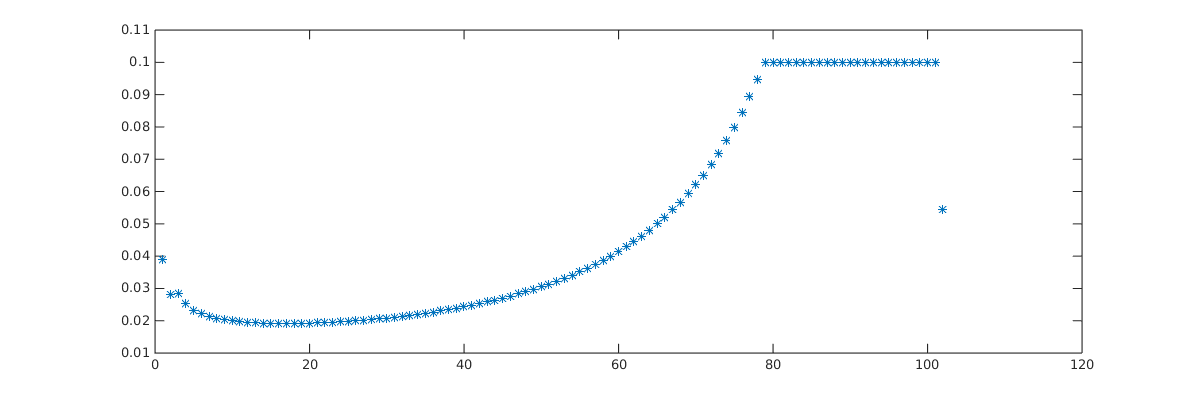
\includegraphics{./7rkf45t.png} \textless{}article\textgreater{} 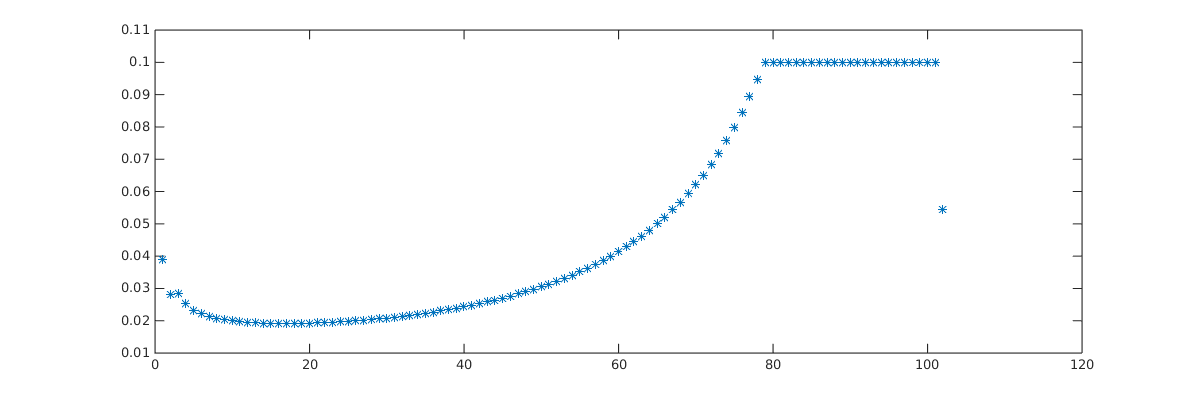
\includegraphics{./7rkf45t.png}
% 
% 
% \section{Runge-Kutta aðferðir – Aðferð Eulers endurbætt}
% \label{kafli06:runge-kutta-aferir-afer-eulers-endurbaett}
% Í aðferð Eulers nálguðum við heildið
% \(\int_0^1 f(t+sh,x(t+sh))\, ds\) með margfeldi af billengdinni og
% fallgildinu í vinstri endapunkti.
% 
% Við getum endurbætt þessa nálgun með því að taka einhverja nákvæmari
% tölulega nálgun á heildinu til dæmis miðpunktsaðferð
% 
% Nálgunarformúlan verður þá
% \begin{gather}
% \begin{split}\int_0^1f(t+sh,x(t+sh))\, ds \approx f(t+\tfrac 12h,x(t+\tfrac 12 h)).\end{split}\notag
% \end{gather}
% Nú er vandamálið að við höfum nálgað \(x(t_{j-1})\) með
% \(w_{j-1}\) en höfum ekkert nálgunargildi á
% \(x(t_{j-1}+\frac 12 h_j)\).
% 
% Við grípum þá til fyrsta stigs Taylor nálgunar
% \begin{gather}
% \begin{split}\begin{aligned}
% x(t_j+\tfrac 12 h_j)&=x(t_{j-1})+x'(t_{j-1})\big(\tfrac 12 h_j \big)
% +\tfrac 12x''(\xi)\big(\tfrac 12 h_j \big)^2\\
% &\approx w_{j-1}+\tfrac 12 h_jf(t_{j-1},w_{j-1}).\end{aligned}\end{split}\notag
% \end{gather}
% Endurbætt aðferð Eulers er þá í tveim skrefum; við reiknum
% \begin{gather}
% \begin{split}\tilde w_j = w_{j-1} + \tfrac 12 h_j f(t_{j-1},w_{j-1})\end{split}\notag
% \end{gather}
% og fáum svo nálgunargildið
% \begin{gather}
% \begin{split}w_j = w_{j-1} + h_jf\left(
%     t_{j-1}+\tfrac 12 h_j,\tilde w_j\right)\end{split}\notag
% \end{gather}
% 
% \subsection{Annað afbrigði af aðferð Eulers – Aðferð Heun}
% \label{kafli06:anna-afbrigi-af-afer-eulers-afer-heun}
% Lítum nú á aðra aðferð þar sem við nálgum heildið með trapisuaðferð.
% \begin{gather}
% \begin{split}\int_0^1f(t+sh,x(t+sh))\, ds \approx
% \tfrac 12 \big(f(t,x(t))+f(t+h,x(t+h))\big).\end{split}\notag
% \end{gather}
% Af þessu leiðir að nálgunarformúlan á að vera
% \begin{gather}
% \begin{split}w_j=w_{j-1}+\tfrac 12h_j\big(f(t_{j-1},w_{j-1})+f(t_j,w_j)\big)\end{split}\notag
% \end{gather}
% Þetta er greinilega óbein aðferð svo við verðum að byrja á nálgun á
% \(w_j\), með
% \begin{gather}
% \begin{split}w_j\approx x(t_j)=x(t_{j-1}+h_j)\approx x(t_{j-1})+h_jx'(t_{j-1})
% =x(t_{j-1})+h_jf(t_{j-1},w_{j-1})\end{split}\notag
% \end{gather}
% Þetta nýja afbrigði af aðferð Eulers nefnist \emph{aðferð Heun}. Hún er í
% tveim skrefum: Við reiknum fyrst
% \begin{gather}
% \begin{split}\tilde w_j = w_{j-1} + h_jf(t_{j-1},w_{j-1})\end{split}\notag
% \end{gather}
% og fáum svo nálgunargildið
% \begin{gather}
% \begin{split}w_j = w_{j-1} + \tfrac 12h_j
% \big(f(t_{j-1},w_{j-1})+f(t_j,\tilde w_j)\big)\end{split}\notag
% \end{gather}
% 
% \subsection{Forsagnar- og leiðréttingaraðferð}
% \label{kafli06:forsagnar-og-leirettingarafer}
% Endurbætt aðferð Eulers og aðferð Heun eru leiðir til þess að vinna úr
% óbeinum aðferðum, þar sem rakningarformúlan fyrir nálgunargildin er af
% gerðinni
% \begin{gather}
% \begin{split}w_j=w_{j-1}+h_j\varphi(f,t_{j-1},t_j,w_{j-1},w_j)\end{split}\notag
% \end{gather}
% og okkur vantar eitthverja nálgun á \(w_j\) til þess að stinga inn í
% hægri hlið þessarar jöfnu. Við skiptum þessu tvö skref:
% 
% Við beitum einhverri beinni aðferð til þess að reikna út
% \begin{gather}
% \begin{split}\tilde w_j=w_{j-1}+h_j\psi(f,t_{j-1},t_j,w_{j-1})\end{split}\notag
% \end{gather}
% Setjum
% \begin{gather}
% \begin{split}w_j=w_{j-1}+h_j\varphi(f,t_{j-1},t_j,w_{j-1},\tilde w_j).\end{split}\notag
% \end{gather}
% 
% \subsection{2. stigs Runge-Kutta-aðferð}
% \label{kafli06:stigs-runge-kutta-afer}
% Lítum aftur á verkefnið
% \begin{gather}
% \begin{split}\left\{
%     \begin{array}{l}
%       x'(t) = f(t,x(t)) \\
%       x(t_0) = x_0
%     \end{array}
%   \right.\end{split}\notag
% \end{gather}
% og skoðum 2. stigs Taylor liðun á lausninni \(x\) í punkti
% \(t\). Innleiðum fyrst smá rithátt til styttingar, setjum
% \begin{gather}
% \begin{split}  x = x(t), \quad f'_t = \frac{\partial f}{\partial t}(t,x(t)), \quad
%     f = f(t,x(t)), \quad f'_x = \frac{\partial f}{\partial x}(t,x(t)).\end{split}\notag\\\begin{split}Keðjureglan gefur\end{split}\notag
% \end{gather}\begin{gather}
% \begin{split}x''(t)=\dfrac d{dt}f(t,x(t))=f'_t+f'_xx'(t)=f'_t+f\,f'_x.\end{split}\notag
% \end{gather}
% Taylor-liðun lausnarinnar er
% \begin{gather}
% \begin{split}\begin{aligned}
%   x(t+h) &= x + hx'(t) + \frac{1}{2} h^2 x''(t) + O(h^3) \\
%   &= x + hf + \frac{1}{2} h^2 ( f'_t + f f'_x ) + O(h^3) \\
%   &= x + \frac{1}{2}hf + \frac{1}{2}h( f + hf'_t + (hf)f'_x) + O(h^3)\end{aligned}\end{split}\notag
% \end{gather}
% Nú sjáum við að síðasti liðurinn er 1. stigs Taylor liðun \(f\) með
% miðju \((t,x)\) skoðuð í punktinum \((t+h,x+hf)\), því
% \begin{gather}
% \begin{split}f(t+h,x + hf) = f + hf'_t + (hf) f'_x + O(h^2)\end{split}\notag
% \end{gather}
% og þar með er
% \begin{gather}
% \begin{split}x(t+h) = x(t) + \frac{1}{2} hf(t,x) + \frac{1}{2} hf(t+h,x+hf) + O(h^3)\end{split}\notag
% \end{gather}
% Við höfum leitt út
% \begin{gather}
% \begin{split}x(t+h) = x(t) + \tfrac{1}{2} hf(t,x) + \tfrac{1}{2} hf(t+h,x+hf) + O(h^3)\end{split}\notag
% \end{gather}
% Þessi formúla liggur til grundvallar 2. stigs Runge-Kutta-aðferð: Með
% henni fáum við nálgunarrunu \(w_0, w_1, w_2, \ldots\) þannig að
% \(w_0=x(0)\) og
% \begin{gather}
% \begin{split}w_j = w_{j-1} + \tfrac{1}{2}(F_1 + F_2), \quad j = 1,2,\ldots\end{split}\notag
% \end{gather}
% þar sem
% \begin{gather}
% \begin{split}F_1 = h_jf(t_{j-1},w_{j-1}),
%   \quad \text{og} \quad
%   F_2 = h_jf(t_j,w_{j-1}+F_1)\end{split}\notag
% \end{gather}
% og eins og alltaf er \(w_j \approx x(t_j)\).
% 
% 
% \subsection{Matlab forrit fyrir 2. stigs Runge-Kutta-aðferð}
% \label{kafli06:matlab-forrit-fyrir-2-stigs-runge-kutta-afer}
% \begin{Verbatim}[commandchars=\\\{\}]
% function w = runge\PYGZus{}kutta\PYGZus{}2(f,t,alpha);
% \PYGZpc{}   w = runge\PYGZus{}kutta\PYGZus{}2(f,t,alpha)
% \PYGZpc{} 2. stigs Runge\PYGZhy{}Kutta aðferð fyrir afleiðuhneppi
% \PYGZpc{}         x\PYGZsq{}(t)=f(t,x(t)), x(0)=alpha.
% \PYGZpc{} Inn fara: f \PYGZhy{} fallið f
% \PYGZpc{}           t \PYGZhy{} vigur með skiptingu á t\PYGZhy{}ás.
% \PYGZpc{}           alpha \PYGZhy{} upphafsgildið í t(1).
% \PYGZpc{} Út koma:  w \PYGZhy{} fylki með nálgunargildunum.
% N = length(t);
% m = length(alpha);
% w = zeros(m,N);
% w(:,1) = alpha;
% for j=2:N
%   h = t(j)\PYGZhy{}t(j\PYGZhy{}1);
%   F1 = h*f(t(j\PYGZhy{}1),w(:,j\PYGZhy{}1));
%   F2 = h*f(t(j),w(:,j\PYGZhy{}1)+F1);
%   w(:,j) = w(:,j\PYGZhy{}1) + (F1+F2)/2;
% end
% \end{Verbatim}
% 
% 
% \subsection{Klassíska fjórða stigs Runge-Kutta aðferðin}
% \label{kafli06:klassiska-fjora-stigs-runge-kutta-aferin}
% Algengasta Runge-Kutta aðferðin er klassíska Runge-Kutta aðferðin. Þetta
% er fjórða stigs aðferð, sem þýðir að staðarskekkjan er \(O(h^5)\) og
% heildarskekkjan er \(O(h^4)\).
% \begin{gather}
% \begin{split}w_{j} = w_{j-1} + \frac 16(k_1 + 2k_2 + 2k_3 + k_4),\end{split}\notag
% \end{gather}
% þar sem
% \begin{gather}
% \begin{split}\begin{aligned}
%   k_1 &= hf(t_{j-1},w_{j-1}) \\
%   k_2 &= hf\left(t_{j-1} + \frac h2,w_{j-1}+ \frac{k_1}2\right) \\
%   k_3 &= hf\left(t_{j-1} + \frac h2,w_{j-1}+ \frac{k_2}2\right) \\
%   k_4 &= hf(t_{j-1} + h,w_{j-1}+ k_3).
%  \end{aligned}\end{split}\notag
% \end{gather}
% Ef \(f(t,x)\) er bara fall af \(t\), þ.e. óháð \(x\), þá
% svarar þetta til þess að meta heildið \({\varphi}\) með
% Simpson-reglunni.
% 
% 
% \subsection{Runge-Kutte 4 prófuð}
% \label{kafli06:runge-kutte-4-profu}
% Skoðum nú sama dæmi og þegar við prófuðum aðferð Eulers.
% 
% Þá gefa eftirfarandi skipanir mynd af skekkjunni.
% 
% \begin{Verbatim}[commandchars=\\\{\}]
% \PYGZgt{}\PYGZgt{} f = @(t,x) t./x;
% \PYGZgt{}\PYGZgt{} [w,t]=rk4(f,0,1,5,100);
% \PYGZgt{}\PYGZgt{} plot(t,sqrt(t.\PYGZca{}2+1) \PYGZhy{} w)
% \end{Verbatim}
% 
% \textless{}presentation\textgreater{} 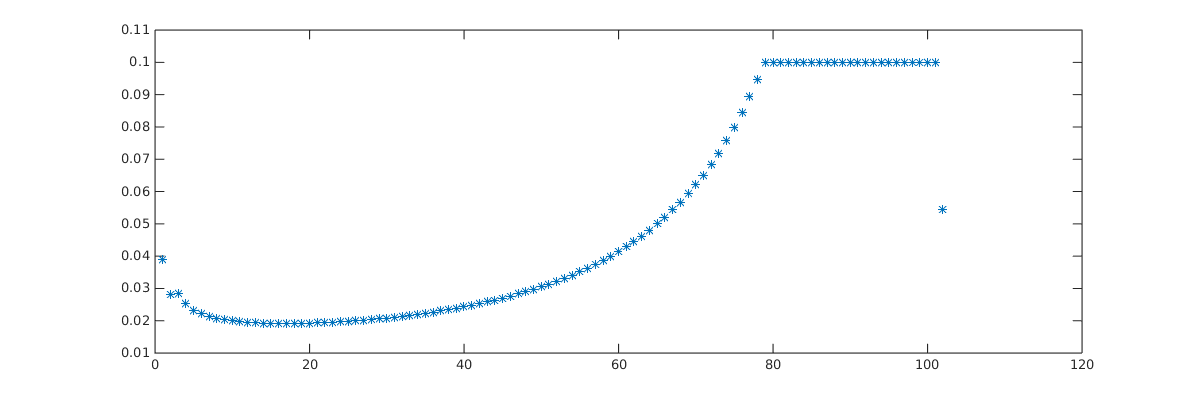
\includegraphics{./7rkf45t.png} \textless{}article\textgreater{} 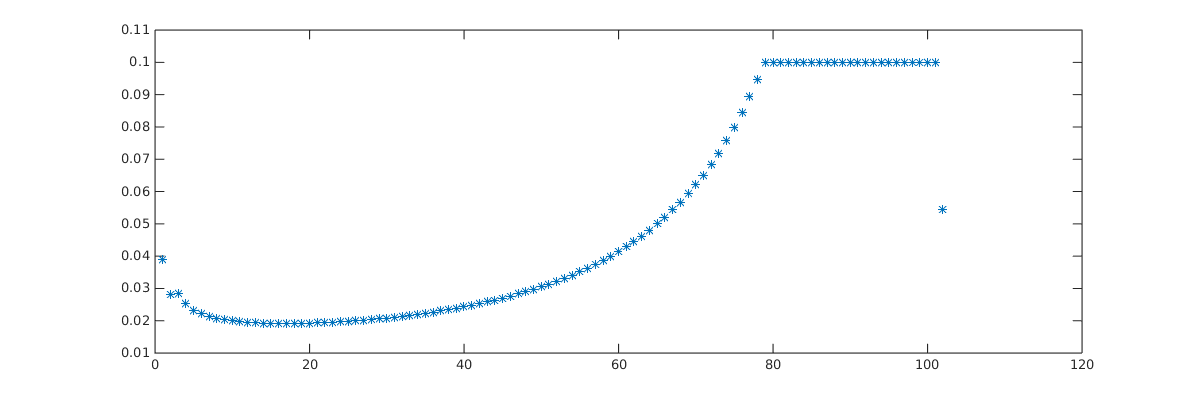
\includegraphics{./7rkf45t.png}
% 
% 
% \section{Skekkjumat, samleitni og stöðugleiki}
% \label{kafli06:skekkjumat-samleitni-og-stougleiki}
% Fyrir eins skrefs aðferð skilgreinum við \emph{staðarskekkju} við tímann
% \(t_n\) sem
% \begin{gather}
% \begin{split}\tau_n = \dfrac{x(t_n)-x(t_{n-1})}{h_n} -
% \varphi(f,t_{n-1},t_n,x(t_{n-1}),x(t_{n}))\end{split}\notag
% \end{gather}
% Hér er réttu lausninni stungið inn í nálgunarformúluna. Munum að hún
% uppfyllir
% \begin{gather}
% \begin{split}\dfrac{x(t_n)-x(t_{n-1})}{h_n}
% =\int_0^1 f(t_{n-1}+sh_n,x(t_{n-1}+sh_n))\, ds\end{split}\notag
% \end{gather}
% Viljum geta metið \(\tau_n\) sem fall af \(h_n\), t.d.
% \begin{gather}
% \begin{split}\tau_n = O(h_n^k)\end{split}\notag
% \end{gather}
% Almennt batna aðferðir eftir því sem veldisvísirinn \(k\) í
% staðarskekkjunni verður stærri.
% 
% 
% \subsection{Staðarskekkja í aðferð Eulers}
% \label{kafli06:staarskekkja-i-afer-eulers}
% Aðferð Eulers er sett fram með formúlunni
% \begin{gather}
% \begin{split}w_n=w_{n-1}+h_nf(t_{n-1},w_{n-1})\end{split}\notag
% \end{gather}
% Staðarskekkjan er því
% \begin{gather}
% \begin{split}\begin{aligned}
%   \tau_n&=\dfrac{x(t_n)-x(t_{n-1})}{h_n}-f(t_{n-1},x(t_{n-1}))\\
% &=\dfrac{x(t_n)-x(t_{n-1})-x'(t_{n-1})h_n}{h_n}\\
% &=\dfrac{\tfrac 12 x''(\xi_{n})h_{n-1}^2}{h_n}
% =\tfrac 12 x''(\xi_{n})h_{n-1}=O(h_n)\end{aligned}\end{split}\notag
% \end{gather}
% Aðferð Eulers er því fyrsta stigs aðferð.
% 
% 
% \subsection{Stýring á staðarskekkju og breytileg skrefastærð}
% \label{kafli06:styring-a-staarskekkju-og-breytileg-skrefastaer}
% Hugsum okkur að við höfum tvær beinar nálgunaraðferðir
% \begin{gather}
% \begin{split}w_{n} = w_{n-1} + h_n\varphi(f,t_{n-1},t_n,w_{n-1})\end{split}\notag
% \end{gather}
% og
% \begin{gather}
% \begin{split}\tilde w_{n} = w_{n-1} + h_n\tilde\varphi(f,t_{n-1},t_n,w_{n-1})\end{split}\notag
% \end{gather}
% Skilgreinum tilsvarandi staðarskekkjur
% \begin{gather}
% \begin{split}\tau_n(h_n) = k_1h_n^{\alpha_1} + o(h_i^{\alpha_1})\end{split}\notag
% \end{gather}
% og
% \begin{gather}
% \begin{split}\tilde\tau_n(h_n) = k_2h_n^{\alpha_2} + o(h_i^{\alpha_2}),\end{split}\notag
% \end{gather}
% þar sem \(\alpha_2>\alpha_1\). Við tímann \(t_{n-1}\) hafa
% nálgunargildin \(w_0,\ldots,w_{n-1}\) hafi verið valin samkvæmt
% fyrri aðferðinni.
% 
% Meiningin að velja næsta tímapunkt \(t_n\) og þar með tímaskref
% \(h_n\) þannig að \(\tau_n(h_n)\leq \delta\), en að
% \(\tau_n(h_n)\) haldi sig sem næst \(\delta\), þar sem
% \(\delta\) er gefið efra mark á staðarskekkjunni í fyrri
% aðferðinni.
% 
% Stærðin \(\delta\) er kölluð \emph{þolmörk} (e. tolerance) fyrir
% staðarskekkjuna og er oft táknuð með \(TOL\).
% 
% Við byrjum á að setja \(h=h_{n}\) inn í báðar aðferðirnar og bera
% útkomurnar saman
% \begin{gather}
% \begin{split}w_{n} = w_{n-1} + h\varphi(f,t_{n-1},t_{n-1}+h,w_{n-1})\end{split}\notag
% \end{gather}\begin{gather}
% \begin{split}\tilde w_{n} = \tilde w_{n-1} +
% h\tilde\varphi(f,t_{n-1},t_{n-1}+h,w_{n-1})\end{split}\notag
% \end{gather}
% Við látum \(\hat w_{n}\) tákna rétt gildi lausnarinnar á
% upphafsgildisverkefninu
% \begin{itemize}
% \item {} 
% \(x'(t)=f(t,x(t))\),
% 
% \item {} 
% \(x(t_{n-1})=w_{n-1}\),
% 
% \end{itemize}
% 
% í punktinum \(t_{n-1}+h\).
% 
% Þá höfum við
% \begin{gather}
% \begin{split}\begin{aligned}
%  \tau_n(h)&=\dfrac{\hat
% w_{n}-w_{n-1}}{h}-\varphi(f,t_{n-1},t_{n-1}+h,w_{n-1})\\
% &=\dfrac{\hat
% w_{n}-w_{n-1}-h\varphi(f,t_{n-1},t_{n-1}+h,w_{n-1})}{h}
% =\dfrac {\hat w_{n}-w_{n}}{h}\end{aligned}\end{split}\notag
% \end{gather}
% og eins fæst
% \begin{gather}
% \begin{split}\begin{aligned}
% \tilde \tau_n(h)
% &=\dfrac{\hat
% w_{n}-w_{n-1}}{h}-\tilde \varphi(f,t_{n-1},t_{n-1}+h,w_{n-1})\\
% &=\dfrac{\hat
% w_{n}-w_{n-1}-h\tilde \varphi(f,t_{n-1},t_{n-1}+h,w_{n-1})}{h}
% =\dfrac {\hat w_{n}-\tilde w_{n}}{h}. \end{aligned}\end{split}\notag
% \end{gather}
% Nú tökum við mismuninn og skilgreinum
% \begin{gather}
% \begin{split}\begin{aligned}
% \varepsilon
% &= \left|\frac{\tilde w_{n}-w_{n}}{h}\right|=|\tau_n(h)-\tilde
%   \tau_n(h)|\\
% &=|k_1|h^{\alpha_1}+o(h^{\alpha_1}) \approx |k_1|h^{\alpha_1}  \end{aligned}\end{split}\notag
% \end{gather}
% Munum að hér er skreflengdin \(h=h_{n}\). Þessi nálgunarformúla
% gefur okkur möguleika á því að meta fastann
% \begin{gather}
% \begin{split}|k_1|\approx
% \dfrac\varepsilon{h_{n}^{\alpha_1}}.\end{split}\notag
% \end{gather}
% 
% \subsection{Mat á skrefastærð}
% \label{kafli06:mat-a-skrefastaer}
% Segjum nú að við viljum halda staðarskekkjunni innan markanna
% \(\delta/2\) og hafa skreflengdina í næsta skrefi
% \(h_{n}=qh_{n-1}\), þá höfum við nálgunarjöfnuna
% \begin{gather}
% \begin{split}|\tau_n(qh_{n-1})|\approx |k_1|(qh_{n-1})^{\alpha_1}=
% \varepsilon {q^{\alpha_1}} \approx  \frac{\delta} 2.\end{split}\notag
% \end{gather}
% Við tökum
% \begin{gather}
% \begin{split}q = \left(\frac{\delta}{2\varepsilon}\right)^{1/{\alpha_1}}\end{split}\notag
% \end{gather}
% veljum síðan skrefstærðina \(h_n = qh_{n-1}\) og reiknum út næsta
% gildi
% \begin{gather}
% \begin{split}w_{n} = w_{n-1} + h_n\varphi(f,t_{n-1},t_n,w_{n-1})\end{split}\notag
% \end{gather}
% 
% \section{Aðferðir með breytilega skrefastærð}
% \label{kafli06:aferir-me-breytilega-skrefastaer}
% Það eru nokkrar aðferðir sem notast við breytilega skrefastærð.
% \begin{itemize}
% \item {} 
% Einfaldast væri að nota Heun aðferðina (annars stigs) til að meta
% skrefastærðina í Euler aðferðinni (fyrsta stigs).
% 
% \item {} 
% Algengasta aðferðin er Runge-Kutta-Fehlberg (RKF45) sem notar
% 5. stigs nálgun til þess að meta staðarskekkjuna í 4. stigs aðferð.
% 
% \item {} 
% Endurbót á RKF45 er Runge-Kutta-Verner (RKV56) sem notar 6. stigs
% aðferð til að meta skekkjuna í 5. stigs aðferð.
% 
% \item {} 
% Fleiri aðferðir: Bogacki–Shampine (3. og 2. stigs), Cash–Karp (5. og
% 4. stigs) og Dormand–Prince (5. og 4. stigs).
% 
% \end{itemize}
% 
% 
% \subsection{Reiknirit fyrir Runge-Kutta-Fehlberg (RKF45)}
% \label{kafli06:reiknirit-fyrir-runge-kutta-fehlberg-rkf45}\begin{gather}
% \begin{split}\begin{aligned}
%   \tilde w_j &= w_{j-1} \frac{16}{135} k_1 + \frac{6656}{12825}k_3 + \frac{28561}{56430}k_4
%   - \frac{9}{50}k_5 + \frac{2}{55}k_6\\
%   w_j &= w_{j-1} + \frac{25}{216}k_1 + \frac{1408}{2565}k_3 + \frac{2197}{4104}k_4 - \frac 15 k_5
%  \end{aligned}\end{split}\notag
% \end{gather}
% þar sem
% \begin{gather}
% \begin{split}\begin{aligned}
%   k_1 &= hf(t_{j-1},w_{j-1}) \\
%   k_2 &= hf\left( t_{j-1}+\frac 14h, w_{j-1}+\frac 14k_1          \right)\\
%   k_3 &= hf\left( t_{j-1}+\frac 38h, w_{j-1}+\frac 3{32}k_1 + \frac 9{32}k_2\right)\\
%   k_4 &= hf\left( t_{j-1}+\frac{12}{13}h, w_{j-1} + \frac{1932}{2197}k_1
%   - \frac{7200}{2197}k_2 + \frac{7296}{2197}k_3 \right)\\
%   k_5 &= hf\left( t_{j-1} +h, w_{j-1} + \frac{439}{216}k_1 - 8k_2+\frac{3680}{513}k_3
%   -\frac{845}{4104}k_4\right)\\
%   k_6 &= hf\left( t_{j-1} +\frac 12h, w_{j-1} - \frac 8{27}k_1 + 2k_2 -\frac{3544}{2565}k_3
%   +\frac{1859}{4104}k_4 - \frac{11}{40}k_5\right)\\
%  \end{aligned}\end{split}\notag
% \end{gather}
% 
% \subsection{Runge-Kutte-Fehlberg (RKF45) prófuð}
% \label{kafli06:runge-kutte-fehlberg-rkf45-profu}
% Notum sama dæmi of þegar við prófuðum aðferð Eulers og RK4.
% 
% Þá gefur eftirfarandi mynd af skekkjunni. Hér er 0.01 minnsta leyfilega
% skrefastærðin, 0.1 stærsta leyfilega skrefastærðin og þolmörkin eru
% \(10^{-10}\).
% 
% \begin{Verbatim}[commandchars=\\\{\}]
% \PYGZgt{}\PYGZgt{} f = @(t,x) t./x;
% \PYGZgt{}\PYGZgt{} [w,t] = rkf45(f,0,1,5,[0.01,0.1,1E\PYGZhy{}10]);
% \PYGZgt{}\PYGZgt{} plot(t,sqrt(t.\PYGZca{}2+1) \PYGZhy{} w)
% \end{Verbatim}
% 
% \textless{}presentation\textgreater{} 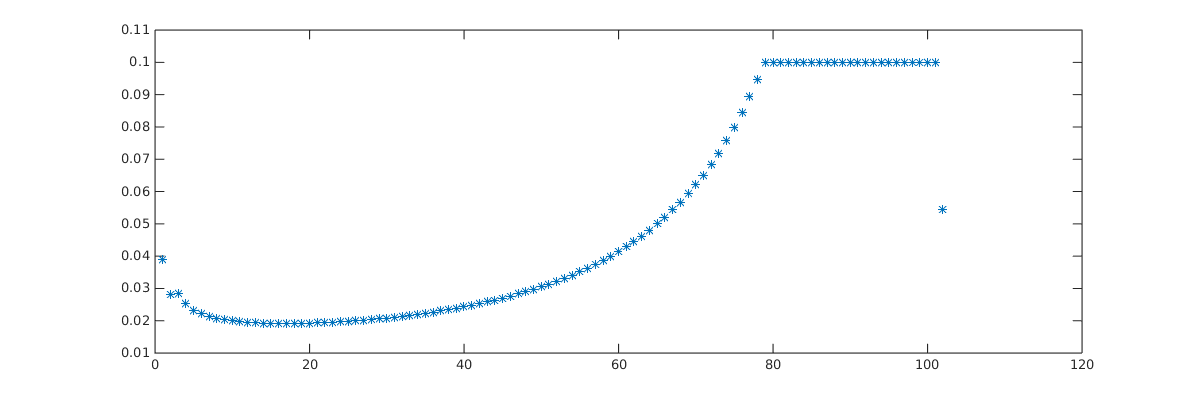
\includegraphics{./7rkf45t.png} \textless{}article\textgreater{} 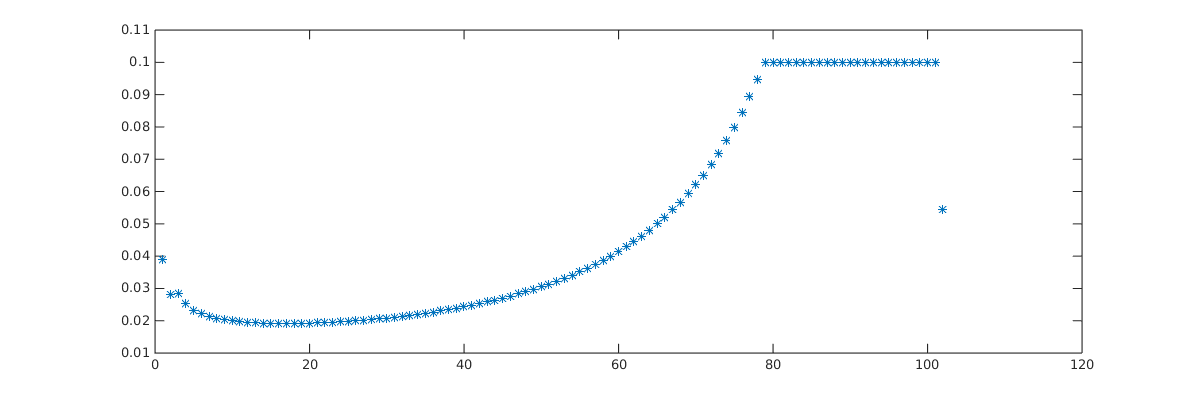
\includegraphics{./7rkf45t.png}
% 
% Hér á undan þá notðum við þolmörkin \(10^{-10}\) sem skilaði okkur
% 103 misstórum tímagildum á bilinu \([0,5]\). Svona getum við teiknað
% upp stærðina á tímaskrefunum.
% 
% \begin{Verbatim}[commandchars=\\\{\}]
% \PYGZgt{}\PYGZgt{} plot(t(2:end)\PYGZhy{}t(1:end\PYGZhy{}1),\PYGZsq{}*\PYGZsq{})
% \end{Verbatim}
% 
% \textless{}presentation\textgreater{} 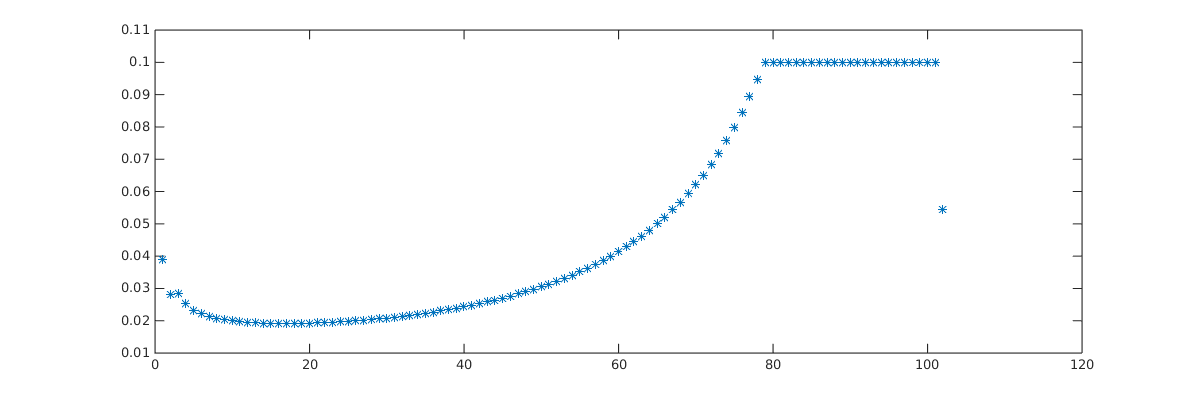
\includegraphics{./7rkf45t.png} \textless{}article\textgreater{} 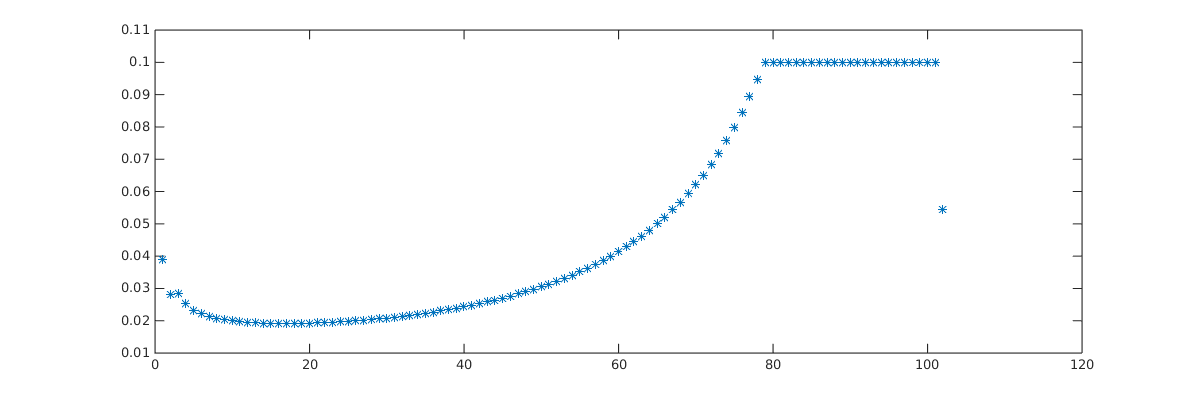
\includegraphics{./7rkf45t.png}
% 
% 
% \section{Fjölskrefaaðferðir}
% \label{kafli06:fjolskrefaaferir}
% Þær aðferðir sem við höfum séð eiga allar sameiginlegt að ákvarða
% nálgunargildi \(w_{n}\) aðeins út frá gildinu \(w_{n-1}\) næst á
% undan. Hægt er að nota fleiri gildi \(w_{n-1}\), \(w_{n-2}\),
% \(\ldots\) og fá þannig betri nákvæmni, en aðferðirnar verða að sama
% skapi flóknari í notkun.
% 
% Eins og alltaf höfum við verkefnið
% \begin{gather}
% \begin{split}\left\{
%     \begin{array}{l}
%       x'(t) = f(t,x(t)) \\
%       x(t_0) = w_0
%     \end{array}
%   \right.\end{split}\notag
% \end{gather}
% og viljum nálga gildi lausnarinnar \(x\) á bili \([a,b]\) þar
% sem \(a =t_0\) eða \(b = t_0\). Látum \(t_0\), \(t_1\),
% \(\ldots\), \(t_n\) vera skiptingu á bilinu \([a,b]\) og
% gerum til einföldunar ráð fyrir að hún hafi jafna billengd
% \(h=t_{j} - t_{j-1}\) fyrir \(j= 1, \ldots, n\).
% 
% 
% \subsection{\(k\)-skrefa Adams-Bashforth aðferð}
% \label{kafli06:skrefa-adams-bashforth-afer}
% Við vitum að lausnin \(x\) uppfyllir
% \begin{gather}
% \begin{split}x(t_{n}) - x(t_{n-1}) =
%   \int\limits_{t_{n-1}}^{t_n} f(t,x(t)) \, dt\end{split}\notag
% \end{gather}
% Skrifum nú
% \begin{gather}
% \begin{split}f(t,x(t)) = P_{k-1}(t) + R_{k-1}(t)\end{split}\notag
% \end{gather}
% þar sem
% \begin{gather}
% \begin{split}P_{k-1}(t) = \sum\limits_{j=1}^k f(t_{n-j},x(t_{n-j})) \cdot
%   \ell_{k-1,j}(t)\end{split}\notag
% \end{gather}
% er brúunarmargliðan gegnum punktana \((t_{n-k},x(t_{n-k}))\),
% \((t_{n+1-k},x(t_{n+1-k}))\), \(\ldots\),
% \((t_{n-1},x(t_{n-1}))\), þ.e. gegnum síðustu \(k\) punkta á
% undan \((t_n,x(t_n))\).
% 
% Þetta eru \(k\) punktar og því er aðferðin kölluð \(k\)-skrefa
% aðferð.
% 
% Munum að til er \(\xi\) þannig að
% \begin{gather}
% \begin{split}R_{k-1}(t) = \frac{f^{(k)}(\xi,x(\xi))}{k!}
%   \prod\limits_{j=1}^m (t-t_{n-j}).\end{split}\notag
% \end{gather}
% Við nálgum nú heildið af \(f\) yfir bilið \([t_{n-1},t_n]\) með
% heildi \(P_{k-1}\) og fáum
% \begin{gather}
% \begin{split}  w_{i+1} = w_i +
%     \int\limits_{t_i}^{t_{i+1}} P_{k-1}(t) \, dt\end{split}\notag\\\begin{split}og með beinum útreikningum má sjá að skekkjan í þessari nálgun er\end{split}\notag
% \end{gather}
% \(O(h^{k+1})\). Þessir útreikninga flækjast auðvitað eftir því sem
% \(k\) stækkar.
% 
% Augljóslega getum við ekki notað \(k\) skrefa Adams-Bashforth
% aðferðir um leið og við sjáum upphafsgildisverkefni, því við þurfum
% \(k\) ágiskunargildi \(w_0, w_1, \ldots, w_{k-1}\) til að byrja
% að nota aðferðina. Þessi gildi má fá með hverri sem er af aðferðunum sem
% við höfum séð hingað til.
% 
% Ákveðin sértilfelli Adams-Bashforth aðferðanna eru meira notuð en önnur,
% það eru tveggja, þriggja og fjögurra skrefa aðferðirnar. Áhugasömum
% verður ekki skotaskuld úr að leiða út formúlurnar fyrir þær, en við
% birtum bara niðurstöðurnar.
% 
% Til styttingar skilgreinum við \(f_j = f(t_j,w_j)\).
% 
% 
% \subsection{Tveggja skrefa Adams-Bashforth-aðferð}
% \label{kafli06:tveggja-skrefa-adams-bashforth-afer}
% Þegar gildin \(w_{n-1}\) og \(w_{j-2}\) hafa verið fundin fæst
% næsta með
% \begin{gather}
% \begin{split}w_{n} = w_{n-1} + h\big(\tfrac 32 f_{n-1} - \tfrac 12 f_{n-2}\big)\end{split}\notag
% \end{gather}
% og skekkjan í nálguninni er \(O(h^3)\).
% 
% 
% \subsection{Forrit fyrir tveggja skrefa Adams-Bashforth-aðferð}
% \label{kafli06:forrit-fyrir-tveggja-skrefa-adams-bashforth-afer}
% Aðferðin er útfærð í forritinu hér að neðan; það skýrir sig að mestu
% sjálft en við skulum taka eftir þrennu:
% 
% (i) Við krefjumst þess að notandinn gefi nálgunargildi á x(t(2)), þetta
% gerum við því til eru margar mismunandi aðferðir til að fá slíkt gildi
% og þær henta mis vel hverju sinni.
% 
% (ii) Við gerum ekki sérstaklega ráð fyrir að jafnt bil sé á milli
% stakanna í vigrinum t þó við höfum gert það hingað til. Það var aðeins
% gert til að einfalda útreikninga; aðferðin virkar nákvæmlega eins ef það
% er ekki jafnt bil á milli stakanna, svo sjálfsagt er að forrita hana
% þannig.
% 
% (iii) Við lágmörkum fjölda skipta sem við reiknum gildi f með að geyma
% alltaf gildið frá síðustu ítrun og nota það aftur, þetta getur sparað
% nokkurn tíma í útreikningum ef f er flókið fall.
% 
% \begin{Verbatim}[commandchars=\\\{\}]
% function w = adams\PYGZus{}bashforth\PYGZus{}2(f,t,x1,x2)
% \PYGZpc{}   w = adams\PYGZob{}\PYGZus{}\PYGZcb{}bashforth\PYGZob{}\PYGZus{}\PYGZcb{}2(f,t,x1,x2)
% \PYGZpc{} Nálgar lausn upphafsgildisverkefnisins
% \PYGZpc{}   x\PYGZsq{} = f(t,x)
% \PYGZpc{}   x(t(1)) = x1
% \PYGZpc{} í punktunum í t með 2ja þrepa Adams\PYGZhy{}Bashforth aðferð.
% \PYGZpc{} Stakið x2 er nálgunargildi á x(t(2)).
% 
% N = length(t);  M = length(x1); w = zeros(M,N);
% \PYGZpc{} Upphafsstillum gildi f(t,x) og w
% fx1 = f(t(1),x1); fx2 = f(t(2),x2);
% w(:,1) = x1; w(:,2) = x2;
% for i=3:N
%   \PYGZpc{} Reiknum nálgunargildi
%   h = t(i)\PYGZhy{}t(i\PYGZhy{}1);
%   w(:,i) = w(:,i\PYGZhy{}1) + (h/2)*(3*fx2 \PYGZhy{} fx1);
%   fx1 = fx2; fx2 = f(t(i),w(:,i));
% end
% \end{Verbatim}
% 
% 
% \subsection{Þriggja skrefa Adams-Bashforth}
% \label{kafli06:riggja-skrefa-adams-bashforth}
% Gefin \(w_{n-1}\), \(w_{n-2}\) og \(w_{n-3}\) fæst næsta
% nálgunargildi með
% \begin{gather}
% \begin{split}w_{n} = w_{n-1} + {h}(\tfrac{23}{12} f_{n-1} - \tfrac {16}{12}
%   f_{n-2} + \tfrac 5{12} f_{n-2})\end{split}\notag
% \end{gather}
% og staðarskekkjan er \(O(h^4)\)
% 
% 
% \subsection{Fjögurra skrefa Adams-Bashforth}
% \label{kafli06:fjogurra-skrefa-adams-bashforth}
% Þegar við þekkjum \(w_{n-1}\), \(w_{n-2}\), \(w_{n-3}\) og
% \(w_{n-4}\) reiknum við næsta gildi með
% \begin{gather}
% \begin{split}w_{n} = w_{n-1} + h\big(\tfrac{55}{24}f_{n-1} - \tfrac{59}{24}f_{n-2} +
% \tfrac {37}{24}f_{n-3} -\tfrac 9{24}f_{n-4}\big)\end{split}\notag
% \end{gather}
% og skekkjan í nálguninni er \(O(h^5)\).
% 
% 
% \section{Greining á samleitni og stöðugleika}
% \label{kafli06:greining-a-samleitni-og-stougleika}
% Lítum aftur á upphafsgildisverkefnið okkar
% \begin{gather}
% \begin{split}\begin{cases}
%   x'(t)=f(t,x(t)),\\
% x(t_0)=w_0.
% \end{cases}\end{split}\notag
% \end{gather}
% Við hugsum okkur að nálgun sé fundin í tímapunktunum
% \begin{gather}
% \begin{split}a=t_0<t_1<t_2<\cdots<t_N=b.\end{split}\notag
% \end{gather}
% Við táknum nálgunargildi á \(x(t_j)\) með \(w_j\). Það er gefið
% með
% \begin{gather}
% \begin{split}w_n=w_{n-1}+h_n\varphi(f,t_{0},\dots,t_n,w_{0},\dots,w_{n})\end{split}\notag
% \end{gather}
% þar sem fallið \(\varphi(f,t_{0},\dots,t_n,w_{0},\dots,w_{n})\) er
% skilgreint með einhverjum hætti.
% 
% Við köllum þetta \emph{nálgunaraðferðina sem fallið} \(\varphi\) \emph{gefur af
% sér.}
% 
% 
% \subsection{Skekkja}
% \label{kafli06:skekkja}
% \emph{Skekkja} (e. error) eða \emph{heildarskekkja} (e. total error) í nálgun á
% \(x(t_n)\) með \(w_n\) er
% \begin{gather}
% \begin{split}e_n=x(t_n)-w_n.\end{split}\notag
% \end{gather}
% (e. local truncation error) nálgunaraðferðarinnar við tímann \(t_n\)
% er
% \begin{gather}
% \begin{split}  \tau_n=\dfrac{x(t_n)-x(t_{n-1})}{h_n}
%   -\varphi(f,t_{0},\dots,t_n,x(t_{0}),\dots,x(t_{n}))\end{split}\notag\\\begin{split}Munið að hér er *rétta lausnin* sett inn í nálgunaraðferðina.\end{split}\notag
% \end{gather}
% 
% \subsection{Samleitni}
% \label{kafli06:samleitni}
% Hugsum okkur nú að fjöldi tímapunktanna \(N\) stefni á óendanlegt.
% Við segjum að nálgunaraðferðin \(\varphi\) sé \emph{samleitin} ef
% \begin{gather}
% \begin{split}\lim_{N\to \infty} \max\limits_{1\leq n\leq N} |e_n|=0\end{split}\notag
% \end{gather}
% þar sem \(e_n=x(t_n)-w_n\) táknar skekkjuna í \(n\)-ta
% tímaskrefinu.
% 
% 
% \subsection{Samræmi}
% \label{kafli06:samraemi}
% Við segjum að nálgunaraðferðin \(\varphi\) \emph{samræmist}
% upphafsgildisverkefninu ef um sérhvern tímapunkt \(t_{n-1}\) gildir
% að
% \begin{gather}
% \begin{split}\begin{gathered}
% \lim_{h_n\to 0}\tau_n\\
% =\lim_{t_n\to t_{n-1}}\bigg(\dfrac{x(t_n)-x(t_{n-1})}{t_n-t_{n-1}}
% -\varphi(f,t_{0},\dots,t_n,x(t_{0}),\dots,x(t_{n}))\bigg)
% =0  \end{gathered}\end{split}\notag
% \end{gather}
% 
% \subsection{Samræmi endurbættu Euler-aðferðarinnar}
% \label{kafli06:samraemi-endurbaettu-euler-aferarinnar}
% Munum að endurbætta Euler-aðferðin er
% \begin{gather}
% \begin{split}w_n=w_{n-1}+h_nf(t_{n-1}+\tfrac 12 h_n,w_{n-1}+\tfrac 12 hf(t_{n-1},w_{n-1}))\end{split}\notag
% \end{gather}
% sem gefur staðarskekkjuna
% \begin{gather}
% \begin{split}\begin{gathered}
% \tau_n=\dfrac{x(t_{n-1}+h_n)-x(t_{n-1})}{h_n}\\
% -f(t_{n-1}+\tfrac 12 h_n,x(t_{n-1})+\tfrac 12 h_nf(t_{n-1},x(t_{n-1}))).
%   \end{gathered}\end{split}\notag
% \end{gather}
% Nú hugsum við okkur að \(t_{n-1}\) sé haldið föstu og látum
% billengdina \(h_n=t_n-t_{n-1}\) stefna á \(0\). Þá fæst
% \begin{gather}
% \begin{split}\lim_{h_n\to 0} \tau_n= x'(t_{n-1})-f(t_{n-1},x(t_{n-1}))=0\end{split}\notag
% \end{gather}
% Þetta segir okkur að endurbætta Euler-aðferðin \textbf{samræmist}
% upphafsgildisverkefninu.
% 
% 
% \subsection{Samræmi beinna eins skrefs aðferða}
% \label{kafli06:samraemi-beinna-eins-skrefs-afera}
% Þessi röksemdafærla alhæfist á allar beinar eins skrefs aðferðir, því
% staðarskekkja þeirra er
% \begin{gather}
% \begin{split}\tau_n=\dfrac{x(t_{n-1}+h_n)-x(t_{n-1})}{h_n}
% -\varphi(f,t_{n-1},t_{n-1}+h_n,x(t_{n-1}))\end{split}\notag
% \end{gather}
% Nú er eðlilegt að gefa sér að \(\varphi\) sé samfellt fall og þá
% verður markgildið af staðarskekkjunni
% \begin{gather}
% \begin{split}\begin{gathered}
% x'(t_{n-1})-\varphi(f,t_{n-1},t_{n-1},x(t_{n-1}))\\
% =f(t_{n-1},x(t_{n-1}))-\varphi(f,t_{n-1},t_{n-1},x(t_{n-1})).\end{gathered}\end{split}\notag
% \end{gather}
% Eins skrefs aðferðin sem fallið \(\varphi\) gefur af sér er því
% stöðug ef og aðeins ef
% \begin{gather}
% \begin{split}\varphi(f,t_{n-1},t_{n-1},x(t_{n-1}))
% =f(t_{n-1},x(t_{n-1})).\end{split}\notag
% \end{gather}
% 
% \subsection{Stöðugleiki}
% \label{kafli06:stougleiki}
% Gerum nú ráð fyrir að upphafsgildinu \(w_0\) sé breytt í
% \(\tilde w_0\) og að \(\tilde x(t)\) uppfylli
% \begin{gather}
% \begin{split}\begin{cases}
%   \tilde x'(t)=f(t,\tilde x(t)),\\
% \tilde x(t_0)=\tilde w_0.
% \end{cases}\end{split}\notag
% \end{gather}
% Lítum síðan á tilsvarandi nálgunarrunu
% \begin{gather}
% \begin{split}\tilde w_n=\tilde w_{n-1}+h_n\varphi(f,t_0,\dots,t_n,\tilde
% w_0,\dots,\tilde w_n).\end{split}\notag
% \end{gather}
% \textbf{Skilgreining} Við segjum að nálgunaraðferðin sem \(\varphi\)
% gefur af sér sé \emph{stöðug} ef til er fall \(k(t)>0\) þannig að
% \begin{gather}
% \begin{split}|\tilde w_n-w_n|\leq k(t_n)|\tilde w_0-w_0|, \qquad n=1,2,3\dots.\end{split}\notag
% \end{gather}
% 
% \subsection{Lipschitz-samfelldni}
% \label{kafli06:lipschitz-samfelldni}
% Rifjum nú upp að við gerum ráð fyrir að fallið \(f(t,x)\) sé
% skilgreint á svæði \(D\) sem inniheldur
% \begin{gather}
% \begin{split}\{(t,x)\in {{\mathbb  R}}^2 \, ;\, a\leq t\leq b, x\in {{\mathbb  R}}\}.\end{split}\notag
% \end{gather}
% Við segjum að \(f\) sé \emph{Lipschitz samfellt á} \(D\) \emph{með tilliti
% til} \(x\) ef til er fasti \(C_f\) þannig að
% \begin{gather}
% \begin{split}|f(t,x)-f(t,y)|\leq C_f|x-y|, \qquad x,y\in {{\mathbb  R}}.\end{split}\notag
% \end{gather}
% Hugsum okkur að \(\varphi(f,s,t,x)\) sé fall sem gefur af sér beina
% eins skrefs nálgunaraðferð fyrir upphafsgildisverkefnið
% \(x'(t)=f(t,x(t))\) með \(x(t_0)=w_0\).
% 
% Við segjum að \(\varphi\) sé \emph{Lipschitz-samfellt með tilliti til}
% \(x\) ef um sérhvert Lipschitz-samfellt fall \(f\), tölur
% \(s,t\in [a,b]\) og \(x,y\in {{\mathbb  R}}\) gildir að til er
% fasti \(L_\varphi\) þannig að
% \begin{gather}
% \begin{split}|\varphi(f,s,t,x)-\varphi(f,s,t,y)|\leq L_\varphi|x-y|, \qquad x,y\in {{\mathbb  R}}.\end{split}\notag
% \end{gather}
% 
% \subsection{Setning um stöðugleika og samleitni}
% \label{kafli06:setning-um-stougleika-og-samleitni}
% Gefum okkur jafna skiptingu á tímabilinu \([a,b]\),
% \(t_n=a+nh\), þar sem \(n=0,1,2,\dots,N\) og \(h=(b-a)/N\).
% 
% Ef fallið \(\varphi\) er Lipschitz-samfellt með tilliti til
% \(x\) með Lipschitz-fastann \(L_\varphi\), þá gildir:
% \begin{enumerate}
% \item {} 
% Eins skrefs aðferðin sem \(\varphi\) gefur af sér er stöðug,
% \begin{gather}
% \begin{split}|\tilde w_n-w_n|\leq e^{L_\varphi(t_n-a)}|\tilde w_0-w_0|, \qquad
% n=1,2,3,\dots.\end{split}\notag
% \end{gather}
% \item {} 
% Ef til eru fastar \(c\) og \(p\) þannig að staðarskekkjan
% uppfyllir \(|\tau_n|\leq c\, h^p\), fyrir öll
% \(n=1,2,3,\dots\) og \(h\in ]0,h_0]\), þá er aðferðin
% samleitin og við höfum
% \begin{gather}
% \begin{split}|e_n|=|x(t_n)-w_n|\leq \dfrac{ch^p}{L_\varphi}
% \bigg(e^{L_\varphi(t_n-a)}-1\bigg).\end{split}\notag
% \end{gather}
% \end{enumerate}
% 
% 
% \section{Fræðilegar spurningar}
% \label{kafli06:fraeilegar-spurningar}\begin{enumerate}
% \item {} 
% Hvernig er hægt að skrifa annars stigs jöfnu \(u''=f(t,u,u')\)
% sem jafngilt hneppi?
% 
% \item {} 
% Hvað er \emph{bein aðferð} fyrir upphafsgildisverkefni?
% 
% \item {} 
% Hvað er \emph{óbein aðferð} fyrir upphafsgildisverkefni?
% 
% \item {} 
% Hvað er \emph{eins skrefs aðferð} fyrir upphafsgildisverkefni?
% 
% \item {} 
% Hvað er \emph{fjölskrefaaðferð} fyrir upphafsgildisverkefni?
% 
% \item {} 
% Hvernig er \emph{aðferð Eulers}?
% 
% \item {} 
% Hvernig er \emph{aðferð Eulers endurbætt}?
% 
% \item {} 
% Hvað er \emph{forsagnar- og leiðréttingaraðferð}?
% 
% \item {} 
% Hvernig er \emph{2. stigs Runge-Kutta aðferð}?
% 
% \item {} 
% Hvernig er \emph{4. stigs Runge-Kutta aðferð}?
% 
% \item {} 
% Hvernig er staðarskekkja í nálgunaraðferð fyrir upphafsgildisverkefni
% skilgreind?
% 
% \item {} 
% Rökstyðjið að staðarskekkja í aðferð Eulers sé \(O(h)\), þar sem
% \(h\) er tímaskrefið.
% 
% \item {} 
% Hvernig er tveggja skrefa Adams-Bashforth-aðferð.
% 
% \item {} 
% Hvað þýðir að nálgunaraðferð fyrir upphafsgildisverkefni sé
% samleitin?
% 
% \item {} 
% Hvað þýðir a nálgunaraðferð samræmist upphafsgildisverkefni?
% 
% \end{enumerate}
% 
% 
 \chapter{Jaðargildisverkefni}
% \label{kafli07:jaargildisverkefni}\label{kafli07::doc}
 \textbf{Í VINNSLU}
% 
% 
% \section{Almenn atriði um jaðargildisverkefni}
% \label{kafli07:almenn-atrii-um-jaargildisverkefni}
% Við ætlum að finna nálgunarlausnir á verkefnum af gerðinni
% \begin{gather}
% \begin{split}\begin{gathered}
%     y''=f(x,y,y'), \qquad a\leq x\leq b,\\
% \alpha_1y(a)+\alpha_2 y'(a)=\alpha_3,\\
% \beta_1 y(b)+\beta_2y'(b)=\beta_3.
%   \end{gathered}\end{split}\notag
% \end{gather}
% Afleiðujafnan er sögð vera línuleg ef hún er á forminu
% \begin{gather}
% \begin{split}y''=p(x)y'+q(x)y+r(x), \qquad x\in [a,b].\end{split}\notag
% \end{gather}
% 
% \subsection{Jaðarskilyrðin nefnast}
% \label{kafli07:jaarskilyrin-nefnast}
% \begin{tabular}{|p{0.317\linewidth}|p{0.317\linewidth}|p{0.317\linewidth}|}
% \hline
% \begin{enumerate}
% \item {} 
% \end{enumerate}
%  & 
% Dirichlet-jaðarskilyrði:
%  & 
% \(y(a)=\alpha\),    \(y(b)=\beta\)
% \\
% \hline & 
% (Fallsjaðarskilyrði:)
%  & \\
% \hline\begin{enumerate}
% \setcounter{enumi}{1}
% \item {} 
% \end{enumerate}
%  & 
% Neumann-jaðarskilyrði:
%  & 
% \(y'(a)=\alpha\),    \(y'(b)=\beta\)
% \\
% \hline & 
% (Afleiðujaðarskilyrði:)
%  & \\
% \hline & 
% (Flæðisjaðarskilyrði:)
%  & \\
% \hline\begin{enumerate}
% \setcounter{enumi}{2}
% \item {} 
% \end{enumerate}
%  & 
% Robin-jaðarskilyrði:
%  & 
% \(\alpha_1y(a)+\alpha_2 y'(a)=\alpha_3\)
% \\
% \hline & 
% (Blandað jaðarskilyrði:)
%  & 
% \(\beta_1 y(b)+\beta_2y'(b)=\beta_3\)
% \\
% \hline &  & 
% \((\alpha_1,\alpha_2)\neq (0,0)\)
% \\
% \hline\end{tabular}
% 
% 
% \begin{DUlineblock}{0em}
% \item[] Athugið að blönduð jaðarskilyrði með \(\alpha_2=0\) (eða
% \(\beta_2=0\))
% \item[] er Dirichlet skilyrði með \(\alpha=\alpha_3/\alpha_1\) (eða
% \(\beta=\beta_3/\beta_1\)).
% \end{DUlineblock}
% 
% \begin{DUlineblock}{0em}
% \item[] Athugið að blandað jaðarskilyrði með \(\alpha_1=0\) (eða
% \(\beta_1=0\))
% \item[] er Neumann skilyrði með \(\alpha=\alpha_3/\alpha_2\) (eða
% \(\beta=\beta_3/\beta_2\)).
% \end{DUlineblock}
% 
% 
% \section{Línulegar jöfnur – Dirichlet-jaðarskilyrði}
% \label{kafli07:linulegar-jofnur-dirichlet-jaarskilyri}
% 
% \subsection{Skiptipunktar / Hnútpunktar}
% \label{kafli07:skiptipunktar-hnutpunktar}
% Gefum okkur jafna skiptingu á bilinu \([a,b]\), \(x_j=a+hj\),
% \(h=(b-a)/N\),
% \begin{gather}
% \begin{split}a=x_0<x_1<x_2<\cdots<x_{N-1}<x_N=b.\end{split}\notag
% \end{gather}
% Við nefnum \(x_j\) \emph{skiptipunkta} eða \emph{hnútpunkta} skiptingarinnar.
% 
% Punktarnir \(a=x_0\) og \(b=x_N\) nefnast \emph{endapunktar}
% skiptingarinnar og \(x_j\), með \(j=1,\dots,N-1\), nefnast
% \emph{innri punktar} skiptingarinnar.
% 
% Í fyrstu atrennu ætlum við aðeins að nálga lausnina fyrir línulegar
% jöfnur,
% \begin{gather}
% \begin{split}y''=p(x)y'+q(x)y+r(x), \qquad x\in [a,b].\end{split}\notag
% \end{gather}
% Við reiknum út nálgun á réttu lausninni \(y(x)\) í hnútpunktunum.
% 
% Rétta gildið í punktinum \(x_j\) táknum við með \(y_j\) og
% nálgunargildið með \(w_j\),
% \begin{gather}
% \begin{split}y_j=y(x_j)\approx w_j.\end{split}\notag
% \end{gather}
% Eins skrifum við
% \begin{gather}
% \begin{split}p_j=p(x_j), \qquad q_j=q(x_j), \qquad  r_j=r(x_j).\end{split}\notag
% \end{gather}
% 
% \subsection{Línulegar afleiðujöfnur:}
% \label{kafli07:linulegar-afleiujofnur}
% Nú leiðum við út nálgunarjöfnur, eina fyrir hvern innri skiptipunkt. Við
% byrjum á því að stinga punkti \(x_j\) inn í afleiðujöfnuna
% \begin{gather}
% \begin{split}\big\{ y''(x)= p(x)y'(x)+q(x)y(x) + r(x)\big\}_{x=x_j}.\end{split}\notag
% \end{gather}
% Næst skiptum við á afleiðum og mismunakvótum i þessari jöfnu,
% \begin{gather}
% \begin{split}\dfrac{y_{j+1}-2y_j+y_{j-1}}{h^2} +O(h^2)
% =p_j\dfrac{y_{j+1}-y_{j-1}}{2h}+q_jy_j+r_j+ O(h^2).\end{split}\notag
% \end{gather}
% Síðan stillum við upp nálgunargildunum í stað réttu gildanna:
% 
% 
% \subsection{Skipt á afleiðum og mismunakvótum}
% \label{kafli07:skipt-a-afleium-og-mismunakvotum}
% Endurtökum réttu jöfnuna
% \begin{gather}
% \begin{split}\dfrac{y_{j+1}-2y_j+y_{j-1}}{h^2} +O(h^2)
% =p_j\dfrac{y_{j+1}-y_{j-1}}{2h}+q_jy_j+r_j+ O(h^2).\end{split}\notag
% \end{gather}
% Nú fellum við niður leifaliðina og setjum nálgunargildin í stað réttu
% gildanna:
% \begin{gather}
% \begin{split}\dfrac{w_{j+1}-2w_j+w_{j-1}}{h^2}
% =p_j\dfrac{w_{j+1}-w_{j-1}}{2h}+q_jw_j+r_j\end{split}\notag
% \end{gather}
% Hér fáum við eina jöfnu fyrir sérhvern innri skiptipunkt
% \(j=1,\dots,N-1\).
% 
% 
% \subsection{Dirichlet-jaðarskilyrði}
% \label{kafli07:dirichlet-jaarskilyri}
% Við erum komin með \(N-1\) nálgunarjöfnu til þess að finna
% \(N+1\) nálgunargildi \(w_0,\dots,w_N\) fyrir
% \(y_0,\dots,y_N\).
% 
% Ef við erum að leysa línulegt jaðargildisverkefni með
% Dirichlet-jaðarskilyrðum,
% \begin{gather}
% \begin{split}\begin{gathered}
%     y''=p(x)y'+q(x)y+r(x), \qquad a\leq x\leq b,\\
% y(a)=\alpha \quad \text{ og } \quad y(b)=\beta,
%   \end{gathered}\end{split}\notag
% \end{gather}
% þá fæst nálgunin með því að leysa línulega jöfnuhneppið
% \begin{gather}
% \begin{split}\begin{aligned}
% w_0&=\alpha,\\
% \dfrac{w_{j+1}-2w_j+w_{j-1}}{h^2}
% &=p_j\dfrac{w_{j+1}-w_{j-1}}{2h}+q_jw_j+r_j, \qquad j=1,\dots,N-1,\\
% w_N&=\beta.  \end{aligned}\end{split}\notag
% \end{gather}
% 
% \subsection{Jafngild framsetning á hneppinu}
% \label{kafli07:jafngild-framsetning-a-hneppinu}
% Við lítum aftur á línulegu nálgunarjöfnurnar
% \begin{gather}
% \begin{split}\dfrac{w_{j+1}-2w_j+w_{j-1}}{h^2}
% =p_j\dfrac{w_{j+1}-w_{j-1}}{2h}+q_jw_j+r_j.\end{split}\notag
% \end{gather}
% Margföldum alla liði með \(-h^2\) og röðum síðan óþekktu stærðunum
% vinstra mengin jafnaðarmerkisins. Þá fæst línulega jöfnuhneppið
% \begin{gather}
% \begin{split}\big(-1-\tfrac 12 h p_j\big)w_{j-1}
% +\big(2+h^2q_j\big) w_j
% +\big(-1+\tfrac 12 h p_j\big)w_{j+1}
% =-h^2\, r_j\end{split}\notag
% \end{gather}
% fyrir \(j=1,2,3,\dots,N-1\).
% 
% 
% \subsection{Línulega jöfnuhneppið á fylkjaformi}
% \label{kafli07:linulega-jofnuhneppi-a-fylkjaformi}\begin{gather}
% \begin{split}A{\mbox{${\bf w}$}}={\mbox{${\bf b}$}}\end{split}\notag
% \end{gather}\begin{gather}
% \begin{split}A=\left[\begin{matrix}
%   1&0\\
%   l_1&d_1&u_1\\
%   &l_2&d_2&u_2\\
%   &&\cdot&\cdot&\cdot \\
%   &&&\cdot&\cdot&\cdot \\
%   &&&&\cdot&\cdot&\cdot \\
%   &&&&&l_{N-2}&d_{N-2}&u_{N-2} \\
%   &&&&&&l_{N-1}&d_{N-1}&u_{N-1} \\
%   &&&&&&&0&1
%   \end{matrix}\right]\end{split}\notag
% \end{gather}
% Þar sem stuðlarnir \(l_j\), \(d_j\) og \(u_j\) eru gefnir
% með
% \begin{gather}
% \begin{split}\begin{aligned}
%   l_j&=-1-\tfrac 12 hp_j\\
% d_j&=2+h^2q_j\\
% u_j&=-1+\tfrac 12 hp_j\end{aligned}\end{split}\notag
% \end{gather}
% 
% \subsection{Óþekktar stærðir og hægri hlið}
% \label{kafli07:oekktar-staerir-og-haegri-hli}\begin{gather}
% \begin{split}{\mbox{${\bf w}$}}=\left[
%   \begin{matrix}
% w_0\\ w_1\\ w_2\\ \cdot\\ \cdot\\ \cdot\\
% w_{N-2}\\ w_{N-1}\\ w_N
% \end{matrix}\right]
% \qquad \text{ og } \qquad
% {\mbox{${\bf b}$}}=\left[
% \begin{matrix}
% \alpha \\ -h^2r_1\\ -h^2r_2\\ \cdot \\ \cdot\\ \cdot\\
% -h^2r_{N-2}\\ -h^2r_{N-1}\\ \beta
% \end{matrix}\right]\end{split}\notag
% \end{gather}
% Þetta jöfnuhneppi er leyst og þar með eru nálgunargildin fundin.
% 
% 
% \section{Línulegar jöfnur – Blönduð jaðarskilyrði}
% \label{kafli07:linulegar-jofnur-blondu-jaarskilyri}
% Við skulum gera ráð fyrir að rétta lausnin \(y(x)\) uppfylli blandað
% jaðarskilyrði í \(x=a\),
% \begin{gather}
% \begin{split}\alpha_1y(a)+\alpha_2 y'(a)=\alpha_3.\end{split}\notag
% \end{gather}
% Til þess að líkja eftir afleiðujöfnunni í punktinum \(x=a\) þá
% hugsum við okkur að við bætum einum punkti \(x_{-1}=a-h\) við og
% látum \(w_f\) tákna ímyndað gildi lausnarinnar í \(x_{-1}\).
% 
% Svona punktur \(x_{-1}\) utan við skiptinguna er kallaður
% \emph{felupunktur} við skiptinguna og ímyndað gildi \(w_f\) í felupunkti
% er kallað \emph{felugildi}.
% 
% Takið eftir því að lausnin er ekki til í felupunktinum, en við reiknum
% eins og \(w_f\) sé gildi hennar þar.
% 
% Mismunajafnan sem líkir eftir afleiðujöfnunni í punktinum \(x_0\) er
% \begin{gather}
% \begin{split}\big(-1-\tfrac 12 hp_0\big)w_f+\big(2+h^2 q_0\big)w_0
% +\big(-1+\tfrac 12 hp_0\big)w_1=-h^2r_0\end{split}\notag
% \end{gather}
% Mismunajafnan sem líkir eftir jaðarskilyrðinu er
% \begin{gather}
% \begin{split}\alpha_1w_0+\alpha_2 \dfrac{w_1-w_f}{2h}=\alpha_3.\end{split}\notag
% \end{gather}
% 
% \subsection{Felugildið leyst út}
% \label{kafli07:felugildi-leyst-ut}
% Jafnan sem líkir eftir jaðarskilyrðinu er:
% \begin{gather}
% \begin{split}\alpha_1w_0+\alpha_2 \dfrac{w_1-w_f}{2h}=\alpha_3.\end{split}\notag
% \end{gather}
% Út úr henni leysum við
% \begin{gather}
% \begin{split}w_f=w_1-\dfrac{2h}{\alpha_2}\big(\alpha_3-\alpha_1w_0\big)\end{split}\notag
% \end{gather}
% Við stingum síðan þessu gildi inn í jöfnuna sem líkir eftir
% afleiðujöfnunni
% \begin{gather}
% \begin{split}\big(-1-\tfrac 12 hp_0\big)w_f+\big(2+h^2 q_0\big)w_0
% +\big(-1+\tfrac 12 hp_0\big)w_1=-h^2r_0\end{split}\notag
% \end{gather}
% Útkoman verður:
% 
% 
% \subsection{Jöfnur fyrir gildin í endapunktum}
% \label{kafli07:jofnur-fyrir-gildin-i-endapunktum}
% Fyrsta jafna hneppisins:
% \begin{gather}
% \begin{split}\bigg(2+h^2q_0-\big(2+hp_0\big)h\dfrac{\alpha_1}{\alpha_2}\bigg)w_0
% -2w_1=-h^2r_0-\big(2+hp_0\big)h\dfrac{\alpha_3}{\alpha_2}.\end{split}\notag
% \end{gather}
% Með því að innleiða felupunkt \(x_{N+1}=b+h\) hægra megin við
% skiptinguna, tilsvarandi felugildi \(w_f\) og leysa saman tvær
% jöfnur, þá fáum við síðustu jöfnu hneppisins :
% \begin{gather}
% \begin{split}-2w_{N-1}
% +\bigg(2+h^2q_N+\big(2-hp_N\big)h\dfrac{\beta_1}{\beta_2}\bigg)w_N
% =-h^2r_N-\big(2-hp_N\big)h\dfrac{\beta_3}{\beta_2}\end{split}\notag
% \end{gather}
% Við erum því aftur komin með \((N+1)\times (N+1)\)-jöfnuhneppi
% 
% 
% \subsection{Hneppið á fylkjaformi}
% \label{kafli07:hneppi-a-fylkjaformi}\begin{gather}
% \begin{split}A{\mbox{${\bf w}$}}={\mbox{${\bf b}$}}\end{split}\notag
% \end{gather}\begin{gather}
% \begin{split}A=\left[\begin{matrix}
% a_{11}&a_{12}\\
% l_1&d_1&u_1\\
% &l_2&d_2&u_2\\
% &&\cdot&\cdot&\cdot \\
% &&&\cdot&\cdot&\cdot \\
% &&&&\cdot&\cdot&\cdot \\
% &&&&&l_{N-2}&d_{N-2}&u_{N-2} \\
% &&&&&&l_{N-1}&d_{N-1}&u_{N-1} \\
% &&&&&&&a_{N+1,N}&a_{N+1,N+1}
% \end{matrix}\right]\end{split}\notag
% \end{gather}
% Þar sem stuðlarnir \(l_j\), \(d_j\) og \(u_j\) fyrir
% \(j=1,2,3\dots,N-1\) eru þeir sömu og áður.
% \begin{gather}
% \begin{split}\begin{aligned}
%   l_j&=-1-\tfrac 12 hp_j\\
% d_j&=2+h^2q_j\\
% u_j&=-1+\tfrac 12 hp_j\end{aligned}\end{split}\notag
% \end{gather}
% 
% \subsection{Fyrsta og síðasta lína hneppisins}
% \label{kafli07:fyrsta-og-siasta-lina-hneppisins}\begin{gather}
% \begin{split}\begin{aligned}
% a_{11}&=
% \begin{cases}
%   1,&\text{Dirichlet í } x=a: \alpha_1\neq 0, \alpha_2=0,\\
% d_0&\text{Neumann í } x=a:  \alpha_1=0, \alpha_2\neq 0,\\
% d_0+2hl_0\alpha_1/\alpha_2&\text{Robin í } x=a:  \alpha_2\neq 0.
% \end{cases} \\
% a_{12}&=
% \begin{cases}
%   0,&\text{Dirichlet í } x=a: \alpha_1\neq 0, \alpha_2=0,\\
% -2,&\text{annars}.
% \end{cases}
% \\
% a_{N+1,N+1}&=
% \begin{cases}
%   1,&\text{Dirichlet í } x=b: \beta_1\neq 0, \beta_2=0,\\
% d_N&\text{Neumann í } x=b:  \beta_1=0, \beta_2\neq 0,\\
% d_N-2hu_N\beta_1/\beta_2&\text{Robin í } x=a:  \beta_2\neq 0.
% \end{cases}
% \\
% a_{N+1,N}&=
% \begin{cases}
%   0,&\text{Dirichlet í } x=b: \beta_1\neq 0, \beta_2=0,\\
% -2&\text{annars}.
% \end{cases}
%   \end{aligned}\end{split}\notag
% \end{gather}
% 
% \subsection{Hægri hlið hneppisins}
% \label{kafli07:haegri-hli-hneppisins}\begin{gather}
% \begin{split}{\mbox{${\bf b}$}}=\left[
% \begin{matrix}
% b_1 \\ -h^2r_1\\ -h^2r_2\\ \cdot \\ \cdot\\ \cdot\\
% -h^2r_{N-2}\\ -h^2r_{N-1}\\ b_{N+1}
% \end{matrix}\right]\end{split}\notag
% \end{gather}\begin{gather}
% \begin{split}b_{1}=
% \begin{cases}
%   \alpha=\alpha_3/\alpha_1,
% &\text{Dirichlet í } x=a: \alpha_1\neq 0, \alpha_2=0,\\
% -h^2r_0+2hl_0\alpha_3/\alpha_2
% &\text{Neumann í } x=a:  \alpha_1=0, \alpha_2\neq 0,\\
% -h^2r_0+2hl_0\alpha_3/\alpha_2&\text{Robin í } x=a:  \alpha_2\neq 0.
% \end{cases}\end{split}\notag
% \end{gather}\begin{gather}
% \begin{split}b_{N+1}=
% \begin{cases}
%   \beta=\beta_3/\beta_1,
% &\text{Dirichlet í } x=a: \beta_1\neq 0, \beta_2=0,\\
% -h^2r_N-2hu_N\beta_3/\beta_2&\text{Neumann í } x=a:  \beta_1=0, \beta_2\neq 0,\\
% -h^2r_N-2hu_N\beta_3/\beta_2&\text{Robin í } x=a:  \beta_2\neq 0.
% \end{cases}\end{split}\notag
% \end{gather}
% 
% \subsection{Samantekt}
% \label{kafli07:samantekt}
% Gildi lausnarinnar \(y(x)\) á línulega jaðargildisverkefninu
% \begin{gather}
% \begin{split}\begin{gathered}
%     y''=p(x)y'+q(x)y+r(x), \qquad a\leq x\leq b,\\
% \alpha_1y(a)+\alpha_2 y'(a)=\alpha_3,\\
% \beta_1 y(b)+\beta_2y'(b)=\beta_3
%   \end{gathered}\end{split}\notag
% \end{gather}
% í punktunum \(x_j=a+jh\), þar sem \(h=(b-a)/N\) og
% \(j=0,\dots,N\), eru nálguð með
% \begin{gather}
% \begin{split}w_j\approx y(x_j)=y_j\end{split}\notag
% \end{gather}
% Dálkvigurinn
% \begin{gather}
% \begin{split}{\mbox{${\bf w}$}}=[w_0,w_1,\dots,w_N]^T\end{split}\notag
% \end{gather}
% er lausn á línulegu jöfnuhneppi
% \(A{\mbox{${\bf w}$}}={\mbox{${\bf b}$}}\).
% 
% Stuðlum \((N+1)\times(N+1)\) fylkisins \(A\) og
% \((N+1)\)-dálkvigursins \({\mbox{${\bf b}$}}\) hefur verið lýst
% hér að framan.
% 
% 
 \chapter{Jöfnuhneppi}
% \label{kafli08:jofnuhneppi}\label{kafli08::doc}
 \textbf{Í VINNSLU}
% 
% 
% \section{Línuleg algebra}
% \label{kafli08:linuleg-algebra}
% 
% \subsection{Línuleg jöfnuhneppi}
% \label{kafli08:linuleg-jofnuhneppi}
% Gefið \(n\times n\) fylki \(A\) og \(n\)-vigur
% \(\mbox{${\bf b}$}\) þá leitum við að vigri \(\mbox{${\bf x}$}\)
% þannig að
% \begin{gather}
% \begin{split}A\mbox{${\bf x}$}= \mbox{${\bf b}$}.\end{split}\notag
% \end{gather}
% 
% \subsection{Lausnir}
% \label{kafli08:lausnir}
% Við höfum almennt tvær leiðir til þess að leysa línuleg jöfnuhneppi:
% \begin{itemize}
% \item {} 
% Gauss-eyðing og innsetning.
% 
% \item {} 
% Reikna andhverfu \(A\), \(A^{-1}\). Þá er
% \begin{gather}
% \begin{split}\mbox{${\bf x}$}= A^{-1}\mbox{${\bf b}$}.\end{split}\notag
% \end{gather}
% \end{itemize}
% 
% 
% \subsection{Fjöldi aðgerða}
% \label{kafli08:fjoldi-agera}\begin{itemize}
% \item {} 
% Gauss-eyðing fyrir \(n\times n\) fylki krefst
% \(\frac 23n^3+\frac 12n^2 -\frac 76n\) reikniaðgerða.
% Innsetningin krefst svo \(n^2\) aðgerða til viðbótar. Samanlagður
% fjöldi aðgerða er því
% \begin{gather}
% \begin{split}\frac 23n^3+\frac 32n^2 -\frac 76n.\end{split}\notag
% \end{gather}
% \item {} 
% Það að reikna \(A^{-1}\) krefst hins vegar \(2n^3-2n^2+n\)
% aðgerða og margföldunin \(A^{-1}b\), krefst \(2n^2-n\)
% aðgerða til viðbótar. Samanlagður fjöldi aðgerða er því
% \begin{gather}
% \begin{split}2n^3.\end{split}\notag
% \end{gather}
% \end{itemize}
% 
% Hér er greinilega gáfulegra að nota Gauss-eyðingu. Almennt þá forðumst
% við eins og mögulegt er að reikna \(A^{-1}\).
% 
% 
% \subsection{Vandamál með stöðugleika}
% \label{kafli08:vandamal-me-stougleika}
% Skoðum jöfnuhneppið
% \begin{gather}
% \begin{split}\left[\begin{array}{ll}
% \varepsilon& 1\\
% 1 & 1
% \end{array}\right] \left[\begin{array}{l}
% x_1\\
% x_2
% \end{array}\right]
% =\left[\begin{array}{l}
% 1\\
% 2
% \end{array}\right]\end{split}\notag
% \end{gather}
% Nákvæm lausn er \(x_1=1+\frac{\varepsilon}{1-\varepsilon},
% x_2=1-\frac{\varepsilon}{1-\varepsilon}\).
% 
% Ef hins vegar \(\varepsilon\) er minna en nákvæmnin í tölvunni sem
% erum að vinna á, þá gefur Gauss-eyðing í tölvu, þar sem eytt er með
% 1. línu, svarið \(x_1 = 0, x_2 = 1\).
% 
% Ef línunum væri víxlað, þá gæfi tölvan hins vegar \(x_1=1, x_2=1\)
% sem er miklu nær réttu svari. Sjá nánar skrána tg14\_03synidaemi.pdf á
% Uglu.
% 
% 
% \subsection{Athugasemd}
% \label{kafli08:athugasemd}
% Það er alveg ljóst að megum ekki framkvæma Gauss-eyðingu blindandi því
% þá geta magnast upp styttingarskekkjur sem skemma lausnina okkar.
% 
% 
% \section{Vending (e. pivoting)}
% \label{kafli08:vending-e-pivoting}
% 
% \subsection{Vandamálið}
% \label{kafli08:vandamali}
% Það sem olli vandræðum í dæminu hér á undan var það að forystustuðull
% fyrstu línunnar var hlutfallslega miklu minni en forystustuðull annarrar
% línu.
% 
% 
% \subsection{Lausnin}
% \label{kafli08:lausnin}
% Lausnin felst í því að víxla á línum þannig að við þurfum ekki að notast
% við litla forystustuðla.
% 
% 
% \subsection{Hlutvending (e. partial pivoting)}
% \label{kafli08:hlutvending-e-partial-pivoting}
% Í grófum dráttum: Í umferð \(i\) í Gauss-eyðingunni þá athugum við
% hvort tölugildi forystustuðla línanna fyrir neðan línu \(i\) eru
% stærri en forystustuðull línu \(i\), ef svo er þá víxlum við á
% þeirri línu og línu \(i\).
% 
% Það er, í \(i\)-tu ítrun Gauss-eyðingar þá látum við
% \(M_i = \max_{i\leq j \leq n} |a_{ji}|\). Ef \(|a_{ii}| < M_i\)
% þá víxlum við á línu \(i\) og fyrstu línunni fyrir neðan sem hefur
% forystustuðul með tölugildi jafnt og \(M_i\). (Þetta þýðir að ef
% \(j_0 = \min\{ j ; i \leq j\leq n \text{ og } a_{ji} = M_i \}\) þá
% víxlum við á línu \(i\) og \(j_0\)).
% 
% 
% \subsection{Vankantar}
% \label{kafli08:vankantar}
% Hlutvending virkar oft vel en getur búið til skekkju þar sem hún tekur
% bara tillit til forystustuðlanna í hverri línu, sjá dæmi kafla 3.2
% (bls. 165).
% 
% 
% \subsection{Sköluð hlutvending (e. scaled partial pivoting)}
% \label{kafli08:skolu-hlutvending-e-scaled-partial-pivoting}
% Skilgreinum vigurinn \(\mbox{${\bf s}$}\) sem heldur utan um
% {}`{}`stærð{}`{}` línanna í \(A\),
% \begin{gather}
% \begin{split}s_i = \max_{1\leq j \leq n} |a_{ij}|.\end{split}\notag
% \end{gather}
% Látum dálkvigurinn \(\mbox{${\bf r}$}\) halda utan um það hvernig
% við umröðum línunum í \(A\). Byrjum með
% \begin{gather}
% \begin{split}\mbox{${\bf r}$}= [1\ 2\ 3\ 4\ \ldots\ n]^T.\end{split}\notag
% \end{gather}
% 
% \subsection{Athugasemd}
% \label{kafli08:id1}
% Við munum uppfæra \(\mbox{${\bf r}$}\) eftir þörfum en breytum ekki
% \(\mbox{${\bf s}$}\) (of dýrt ef \(n\) er stórt).
% 
% Í ítrun \(i\) þá látum við
% \begin{gather}
% \begin{split}M_i = \max_{i \leq j \leq n} \frac{|a_{{r_j}i}|}{s_{r_j}},\end{split}\notag
% \end{gather}
% og látum \(j_0\) vera minnsta \(j\) þannig að hámarkinu er náð,
% \begin{gather}
% \begin{split}\frac{ |a_{r_{j_0}i}|}{s_{r_{j_0}}} = M_i.\end{split}\notag
% \end{gather}
% Ef \(i < j_0\) þá skiptum við á línum \(i\) og \(j_0\), þ.e.
% \begin{gather}
% \begin{split}\mbox{${\bf r}$}= [\ldots\ i\ \ldots\ j_0\ \ldots]^T \text{ breytist í }
% \mbox{${\bf r}$}= [\ldots\ j_0\ \ldots\ i\ \ldots]^T.\end{split}\notag
% \end{gather}
% 
% \section{Fylkjastaðall}
% \label{kafli08:fylkjastaall}
% 
% \subsection{Að mæla fjarlægð milli hluta}
% \label{kafli08:a-maela-fjarlaeg-milli-hluta}
% Á rauntalnalínunni þá mælum við fjarlægð með tölugildinu, þannig að
% fjarlægðin á milli \(x\) og \(y\) er gefin með
% \(d(x,y)=|x-y|\).
% 
% Í \({\mathbb  R}^n\) þá finnst okkur evklíðski staðallinn
% náttúrulegur, enda svarar hann til þess að mæla fjarlægð milli punkta
% með reglustiku;
% \begin{gather}
% \begin{split}d(\mbox{${\bf x}$},\mbox{${\bf y}$}) = \sqrt{ (x_1-y_1)^2 + \ldots + (x_n-y_n)^2 }.\end{split}\notag
% \end{gather}
% Þetta er hins vegar ekki eina leiðin til þess mæla fjarlægð í
% \({\mathbb  R}^n\), eins og við sjáum fljótlega, og ekki endilega
% réttari en aðrar aðferðir.
% 
% Almennt viljum við geta mælt ”fjarlægð{}`{}` á milli allra þeirra hluta
% sem við erum skoða, hvort sem það eru margliður, föll eða fylki.
% Tilgangurinn er að geta metið hversu langt nálgunin okkar er frá réttu
% gildi og hversu stór skekkjan er í samanburði við stærð hlutarins sem
% við erum að vinna með.
% 
% 
% \subsection{Vigurstaðall}
% \label{kafli08:vigurstaall}
% 
% \paragraph{Skilgreining}
% \label{kafli08:skilgreining}
% Fall \(\| \cdot\|:{\mathbb  R}^n \to {\mathbb  R}\) kallast
% \emph{vigurstaðall} (e. vector norm) ef fyrir öll
% \(\mbox{${\bf x}$},\mbox{${\bf y}$}\in {\mathbb  R}^n\) og
% \(\alpha \in {\mathbb  R}\) gildir eftirfarandi:
% \begin{enumerate}
% \item {} 
% \(\|\mbox{${\bf x}$}\| \geq 0\)
% 
% \item {} 
% \(\|\mbox{${\bf x}$}\| = 0\) ef og aðeins ef
% \(\mbox{${\bf x}$}= 0\)
% 
% \item {} 
% \(\|\alpha\mbox{${\bf x}$}\| = |\alpha|\|\mbox{${\bf x}$}\|\)
% 
% \item {} 
% \(\|\mbox{${\bf x}$}+\mbox{${\bf y}$}\| \leq \|\mbox{${\bf x}$}\| + \|\mbox{${\bf y}$}\|\)
% 
% \end{enumerate}
% 
% 
% \paragraph{Athugasemd}
% \label{kafli08:id2}
% Tölugildisfallið á \({\mathbb  R}\) er greinilega staðall.
% 
% 
% \subsection{Dæmi um staðla}
% \label{kafli08:daemi-um-stala}
% 
% \paragraph{\(\ell_2\) staðallinn}
% \label{kafli08:staallinn}
% Einnig kallaður evklíðska fjarlægðin, er gefinn með
% \begin{gather}
% \begin{split}\|\mbox{${\bf x}$}\|_2 = \left( \sum_{j=1}^n x_j^2 \right)^{\frac 12} = \sqrt{\mbox{${\bf x}$}\cdot \mbox{${\bf x}$}}.\end{split}\notag
% \end{gather}
% 
% \paragraph{\(\ell_\infty\) staðallinn}
% \label{kafli08:id3}\begin{gather}
% \begin{split}\|\mbox{${\bf x}$}\|_\infty = \max_{1\leq j \leq n} |x_j|.\end{split}\notag
% \end{gather}
% 
% \paragraph{\(\ell_p\) staðlar}
% \label{kafli08:stalar}
% Almennt, ef \(1\leq p < \infty\), þá skilgreinum við
% \begin{gather}
% \begin{split}\|\mbox{${\bf x}$}\|_p = \left( \sum_{j=1}^n |x_j|^p \right)^{\frac 1p}.\end{split}\notag
% \end{gather}
% 
% \subsection{Skilgreining}
% \label{kafli08:id4}
% \emph{Fylkjastaðall} (e. matrix norm) er fall
% \(\|\cdot\|:{\mathbb  R}^{n\times n} \to {\mathbb  R}\), þannig að
% fyrir öll \(A,B \in {\mathbb  R}^{n\times n}\) og
% \(\alpha \in {\mathbb  R}\) gildir
% \begin{enumerate}
% \item {} 
% \(\|A\| \geq 0\)
% 
% \item {} 
% \(\|A\| = 0\) ef og aðeins ef \(A=0\)
% 
% \item {} 
% \(\| \alpha A\| = |\alpha|\|A\|\)
% 
% \item {} 
% \(\|A+B\| \leq \|A\| + \|B\|\)
% 
% \item {} 
% \(\|AB\| \leq \|A\|\|B\|\)
% 
% \end{enumerate}
% 
% 
% \subsection{Athugasemd}
% \label{kafli08:id5}
% Ef þessi skilgreining er borin saman við skilgreininguna á staðli fyrir
% vigurrúm þá sjáum við að eini raunverulegi munurinn er skilyrði 5.
% 
% 
% \subsection{Fylkjastaðall skilgreindur út frá vigurstaðli}
% \label{kafli08:fylkjastaall-skilgreindur-ut-fra-vigurstali}
% 
% \paragraph{Skilgreining}
% \label{kafli08:id6}
% Látum \(\|\cdot\|\) vera vigurstaðal. Fallið
% \(\|\cdot\|:{\mathbb  R}^{n\times n} \to {\mathbb  R}\) sem
% skilgreint er með
% \begin{gather}
% \begin{split}\|A\| = \max_{\|\mbox{${\bf x}$}\| \neq 0} \frac{\|A\mbox{${\bf x}$}\|}{\|\mbox{${\bf x}$}\|},\end{split}\notag
% \end{gather}
% kallast \emph{náttúrulegi fylkjastaðallinn} sem \(\|\cdot\|\) gefur af
% sér.
% 
% 
% \paragraph{Athugasemd}
% \label{kafli08:id7}
% Það þarf að sýna, og er ekki mjög erfitt, að þessi fylkjastaðall
% uppfyllir öll skilyrðin í skilgreiningu hér á undan og er því sannarlega
% fylkjastaðall.
% 
% 
% \paragraph{Athugasemd}
% \label{kafli08:id8}
% Ef \(\|\cdot\|\) er náttúrulegur fylkjastaðall þá gildir að fyrir
% öll fylki \(A\) og alla vigra \(\mbox{${\bf x}$}\) að
% \begin{gather}
% \begin{split}\underbrace{\|A\mbox{${\bf x}$}\|}_{\text{vigurstaðll}} \leq \underbrace{\|A\|}_{\text{fylkjastaðall}}
% \underbrace{\|\mbox{${\bf x}$}\|}_{\text{vigurstaðall}}.\end{split}\notag
% \end{gather}
% 
% \subsection{Dæmi um fylkjastaðal}
% \label{kafli08:daemi-um-fylkjastaal}
% 
% \paragraph{Athugasemd}
% \label{kafli08:id9}
% Fyrir sérhvern \(\ell_p\) staðal fáum við fylkjastaðal
% \(\|\cdot\|_p\).
% 
% 
% \paragraph{\(\|\cdot\|_\infty\)}
% \label{kafli08:id10}
% Einfaldastur er staðallinn sem tilheyrir \(\ell_\infty\), en hann
% uppfyllir
% \begin{gather}
% \begin{split}\|A\|_\infty = \max_{1\leq i \leq n} \sum_{j=1}^n |a_{ij}|.\end{split}\notag
% \end{gather}
% 
% \subsection{Eigingildi}
% \label{kafli08:eigingildi}
% Látum \(A\) vera fylki. Ef tala \(\lambda\) (hugsanlega
% tvinntala) og vigur \(\mbox{${\bf x}$}\) uppfylla
% \begin{gather}
% \begin{split}A\mbox{${\bf x}$}= \lambda \mbox{${\bf x}$},\end{split}\notag
% \end{gather}
% þá kallast \(\lambda\) \emph{eigingildi} \(A\), og
% \(\mbox{${\bf x}$}\) \emph{eiginvigur} \(A\).
% 
% Athugið að eigingildi \(A\) eru nákvæmlega rætur kennimargliðu
% \(A\), \(t \mapsto \det(A-It)\).
% 
% 
% \subsection{Róf og eiginleikar þess}
% \label{kafli08:rof-og-eiginleikar-ess}
% 
% \paragraph{Skilgreining}
% \label{kafli08:id11}
% Mengi allra eigingilda \(A\) er kallað \emph{róf} \(A\) (e. spectrum)
% og er táknað með \(\sigma(A)\).
% 
% \emph{Rófgeisli} (e. spectral radius) fylkisins \(A\) er talan
% \begin{gather}
% \begin{split}\rho(A) = \max_{\lambda \in \sigma(A)} |\lambda|.\end{split}\notag
% \end{gather}
% 
% \paragraph{Setning}
% \label{kafli08:setning}
% Látum \(A\) vera fylki, þá gildir eftirfarandi
% \begin{itemize}
% \item {} 
% \(\|A\|_2 = \sqrt{\rho(A^T A)}\)
% 
% \item {} 
% \(\rho(A) \leq \|A\|\) fyrir sérhvern náttúrulegan fylkjastaðal
% \(\|\cdot\|\)
% 
% \item {} 
% Fyrir sérhvert \(\varepsilon>0\) þá er til náttúrulegur
% fylkjastaðall \(\|\cdot\|\) þannig að
% \(\|A\| \leq \rho(A) + \varepsilon\).
% 
% \end{itemize}
% 
% 
% \section{Skekkjumat og ástandstala}
% \label{kafli08:skekkjumat-og-astandstala}
% 
% \subsection{Hvernig á að mæla skekkju}
% \label{kafli08:hvernig-a-a-maela-skekkju}
% Gerum ráð fyrir að \(A\) sé andhverfanlegt fylki,
% \(\mbox{${\bf b}$}\) vigur og að við séum að leita að lausn
% \(\mbox{${\bf x}$}\) á
% \begin{gather}
% \begin{split}A\mbox{${\bf x}$}= \mbox{${\bf b}$}.\end{split}\notag
% \end{gather}
% Ef við höfum nálgun \(\tilde \mbox{${\bf x}$}\) þannig að \emph{leifin}
% (e. residual)
% \(\mbox{${\bf r}$}= A\tilde \mbox{${\bf x}$}- \mbox{${\bf b}$}\) er
% lítil, hvað getum við þá sagt um \emph{skekkjuna} (e. error)
% \(\mbox{${\bf e}$}= \mbox{${\bf x}$}-\tilde \mbox{${\bf x}$}\)? Er
% hún endilega lítil?
% 
% Sjáum að svo er ekki, skekkjan getur verið hlutfallslega miklu meiri
% heldur en leifin (Example 3.11).
% 
% 
% \subsection{Skekkjumat}
% \label{kafli08:skekkjumat}
% Við höfum fjórar jöfnur
% \begin{gather}
% \begin{split}\mbox{${\bf b}$}=A\mbox{${\bf x}$}, \quad \mbox{${\bf x}$}=A^{-1}\mbox{${\bf b}$}, \quad
% \mbox{${\bf r}$}=A(\mathbf{\tilde x}-\mbox{${\bf x}$})=A\mbox{${\bf e}$}, \quad \text{ og } \quad
% \mbox{${\bf e}$}=A^{-1}\mbox{${\bf r}$}\end{split}\notag
% \end{gather}
% og þær gefa okkur fjórar ójöfnur fyrir tilsvarandi staðal:
% \begin{gather}
% \begin{split}\|\mbox{${\bf b}$}\|\leq \|A\|\|\mbox{${\bf x}$}\|, \quad  \|\mbox{${\bf x}$}\|\leq \|A^{-1}\|\|\mbox{${\bf b}$}\|,
% \quad
% \|\mbox{${\bf r}$}\|\leq \|A\|\|\mbox{${\bf e}$}\|, \quad  \|\mbox{${\bf e}$}\|\leq \|A^{-1}\|\|\mbox{${\bf r}$}\|\end{split}\notag
% \end{gather}
% Við getum tengt tvær síðustu ójöfnurnar saman í mat á skekkjunni
% \begin{gather}
% \begin{split}\dfrac 1{\|A\|}\cdot  \|\mbox{${\bf r}$}\|
% \leq  \|\mbox{${\bf e}$}\| \leq
% \|A^{-1}\| \|\mbox{${\bf r}$}\|\end{split}\notag
% \end{gather}
% og með því að nota fyrstu tvær ójöfnurnar fæst mat á hlutfallslegri
% skekkju
% \begin{gather}
% \begin{split}\dfrac 1{\|A\|\|A^{-1}\|}\dfrac{ \|\mbox{${\bf r}$}\|}{\|\mbox{${\bf b}$}\|}
% \leq \dfrac{\|\mbox{${\bf e}$}\|}{\|\mbox{${\bf x}$}\|} \leq
% \|A\|\|A^{-1}\|\dfrac{\|\mbox{${\bf r}$}\|}{\|\mbox{${\bf b}$}\|}\end{split}\notag
% \end{gather}
% Nú skilgreinum við \emph{ástandstölu fylkisins} \(A\) með
% \begin{gather}
% \begin{split}\kappa(A)=\|A\|\|A^{-1}\|.\end{split}\notag
% \end{gather}
% 
% \subsection{Ástandstala fylkis og mat á hlutfallslegri skekkju}
% \label{kafli08:astandstala-fylkis-og-mat-a-hlutfallslegri-skekkju}
% 
% \paragraph{Matið}
% \label{kafli08:mati}
% Með ástandstölunni verður mat okkar á hlutfallslegu skekkjunum að
% \begin{gather}
% \begin{split}\dfrac 1{\kappa(A)}\cdot \dfrac{ \|\mbox{${\bf r}$}\|}{\|\mbox{${\bf b}$}\|}
% \leq \dfrac{\|\mbox{${\bf e}$}\|}{\|\mbox{${\bf x}$}\|} \leq
% \kappa(A)\cdot \dfrac{\|\mbox{${\bf r}$}\|}{\|\mbox{${\bf b}$}\|}\end{split}\notag
% \end{gather}
% 
% \paragraph{Athugasemd}
% \label{kafli08:id12}
% Athugið að skilgreiningin
% \begin{gather}
% \begin{split}\kappa(A)=\|A\|\|A^{-1}\|.\end{split}\notag
% \end{gather}
% er \emph{mjög} háð því hvaða staðal við veljum, en við höfum þó að
% \begin{gather}
% \begin{split}1=\|I\|=\|AA^{-1}\|\leq \|A\|\|A^{-1}\|=\kappa(A)\end{split}\notag
% \end{gather}
% 
% \subsection{Áhrif gagnaskekkju}
% \label{kafli08:ahrif-gagnaskekkju}
% Hugsum okkur nú að við viljum leysa jöfnuhneppi
% \(A\mbox{${\bf x}$}=\mbox{${\bf b}$}\), en vegna skekkju í stuðlum
% jöfnuhneppisins leysum við annað hneppi
% \(\tilde A\mathbf {\tilde x}=\mathbf{\tilde b}\).
% 
% Við skilgreinum \emph{gagnaskekkjur} \(\delta A=\tilde A-A\) og
% \(\delta\mbox{${\bf b}$}=\mathbf{\tilde b}-\mbox{${\bf b}$}\) og
% ætlum að nota þær til þess að meta skekkjuna
% \(\mbox{${\bf e}$}=\delta\mbox{${\bf x}$}=\mathbf{\tilde x}-\mbox{${\bf x}$}\).
% 
% Við verðum að gera ráð fyrir að \(\|\delta A\|\leq 1/\|A^{-1}\|\)
% sem tryggir að fylkið \(\tilde A\) sé andhverfanlegt.
% 
% Nú stillum við upp jöfnuhneppinu
% \(\tilde A\mathbf{\tilde x}=\mathbf{\tilde  b}\) á forminu
% \begin{gather}
% \begin{split}(A+\delta A)(\mbox{${\bf x}$}+\delta \mbox{${\bf x}$})=(\mbox{${\bf b}$}+\delta\mbox{${\bf b}$})\end{split}\notag
% \end{gather}
% sem jafngildir
% \begin{gather}
% \begin{split}\delta\mbox{${\bf x}$}=A^{-1}\big(\delta\mbox{${\bf b}$}-(\delta A)\mbox{${\bf x}$}-(\delta A)(\delta x)\big)\end{split}\notag
% \end{gather}
% Af þessari jöfnu leiðir ójafnan
% \begin{gather}
% \begin{split}\|\delta\mbox{${\bf x}$}\|\leq
% \|A^{-1}\|\big(\|\delta\mbox{${\bf b}$}\|+\|\delta A\|\|\mbox{${\bf x}$}\|+\|\delta A\|\|\delta \mbox{${\bf x}$}\|\big)\end{split}\notag
% \end{gather}
% Einangrum nú \(\|\delta \mbox{${\bf x}$}\|\),
% \begin{gather}
% \begin{split}\|\delta\mbox{${\bf x}$}\|\leq
% \dfrac{\|A^{-1}\|}{1-\|A^{-1}\|\|\delta A\|}\cdot
% \big(\|\delta\mbox{${\bf b}$}\|+\|\delta A\|\|\mbox{${\bf x}$}\|\big)\end{split}\notag
% \end{gather}
% deilum með \(\|\mbox{${\bf x}$}\|\) báðum megin, margföldum síðan
% með \(\|A\|\) í teljara og nefnara í hægri hliðinni,
% \begin{gather}
% \begin{split}\dfrac{\|\delta\mbox{${\bf x}$}\|} {\|\mbox{${\bf x}$}\|}\leq
% \dfrac{\|A\|\|A^{-1}\|}{1-\|A^{-1}\|\|\delta A\|}\cdot
% \bigg(\dfrac{\|\delta\mbox{${\bf b}$}\|}{\|A\|\|\mbox{${\bf x}$}\|}+
% \dfrac{\|\delta A\|}{\|A\|}\bigg)\end{split}\notag
% \end{gather}
% Samkvæmt skilgreiningu er \(\kappa(A)=\|A\|\|A^{-1}\|\) og við höfum
% auk þess ójöfnuna
% \(\|\mbox{${\bf b}$}\|\leq \|A\|\|\mbox{${\bf x}$}\|\), en það gefur
% matið á hlutfallslegu skekkjunni sem við sækjumst eftir
% \begin{gather}
% \begin{split}\dfrac{\|\delta\mbox{${\bf x}$}\|} {\|\mbox{${\bf x}$}\|}\leq
% \dfrac{\kappa(A)}{1-\kappa(A)\cdot(\|\delta A\|/\|A\|)}\cdot
% \bigg(\dfrac{\|\delta\mbox{${\bf b}$}\|}{\|\mbox{${\bf b}$}\|}+
% \dfrac{\|\delta A\|}{\|A\|}\bigg).\end{split}\notag
% \end{gather}
% 
% \section{LU-þáttun}
% \label{kafli08:lu-attun}
% 
% \subsection{Nokkrar skilgreiningar}
% \label{kafli08:nokkrar-skilgreiningar}\begin{enumerate}
% \item {} 
% Fylkið \(A\) nefnist \emph{neðra þríhyrningsfylki} ef öll stök fyrir
% ofan hornalínuna í \(A\) eru \(0\), þ.e. \(a_{ij}=0\)
% ef \(i<j\).
% 
% \item {} 
% Fylkið \(A\) nefnist \emph{efra þríhyrningsfylki} ef öll stökin neðan
% við hornalínuna eru \(0\), þ.e. \(a_{ij}=0\) ef
% \(i>j\).
% 
% \item {} 
% Fylkið \(A\) nefnist \emph{bandfylki} (e. striped matrix) ef til er
% \(\beta \leq n-2\) þannig að \(a_{ij}=0\) ef
% \(|i-j|>\beta\). Minnsta talan \(\beta\) sem uppfyllir þetta
% skilyrði kallst á \emph{bandvídd} fylkisins \(A\).
% 
% \item {} 
% Ef \(A\) er bandfylki með bandvíddina \(1\), þá nefnist
% \(A\) \emph{þríhornalínufylki}.
% 
% \item {} 
% Fylkið \(A\) er sagt vera {\color{red}\bfseries{}*}samhverft * ef \(a_{ij}=a_{ji}\)
% fyrir öll \(i\) og \(j\).
% 
% \item {} 
% Fylkið \(A\) er sagt vera {\color{red}\bfseries{}*}jákvætt ákvarðað * ef
% \(\mbox{${\bf x}$}^TA\mbox{${\bf x}$}>0\) gildir fyrir alla vigra
% \(\mbox{${\bf x}$}\neq 0\) í \({\mathbb  R}^n\).
% 
% \end{enumerate}
% 
% 
% \subsection{Úrlausn á jöfnuhneppi með neðra þríhyrningsfylki}
% \label{kafli08:urlausn-a-jofnuhneppi-me-nera-rihyrningsfylki}
% Ef \(A\) er neðra þríhyrningsfylki, þá er úrlausn jöfnuhneppisins
% \(A\mbox{${\bf x}$}= \mbox{${\bf b}$}\) auðveld, því hneppið er þá
% af gerðinni
% \begin{gather}
% \begin{split}\begin{aligned}
% {2}
%     &a_{11}x_1&&=b_1,\\
%     &a_{21}x_1+a_{22}x_2&&=b_2,\\
%     &a_{31}x_1+a_{32}x_2+a_{33}x_3&&=b_3,\\
%     &\vdots \qquad \qquad   \vdots \qquad
%     \qquad \vdots& \qquad& \vdots\\
%     &a_{n1}x_1+a_{n2}x_2+a_{n3}x_3\cdots+a_{nn}x_n&&=b_n,\end{aligned}\end{split}\notag
% \end{gather}
% Við getum rakið okkur niður línurnar og leyst úr stærðirnar
% \(x_1,\dots,x_n\) hverja á eftir annarri
% \begin{gather}
% \begin{split}\begin{aligned}
%     x_1& = b_1/a_{11},\\
%     x_2& = (b_2-a_{21}x_1)/a_{22},\\
%     x_3& = (b_3-a_{31}x_1-a_{32}x_2)/a_{33}\\
%     &\vdots \qquad \qquad \vdots \qquad \qquad \vdots\\
%     x_n& = (b_n-a_{n1}x_1-a_{n2}x_2-\cdots
%         -a_{n,n-1}x_{n-1})/a_{nn}.\end{aligned}\end{split}\notag
% \end{gather}
% 
% \subsection{Talning á aðgerðunum við úrlausnina}
% \label{kafli08:talning-a-agerunum-vi-urlausnina}
% Nú skulum við telja saman fjölda reikningsaðgerða sem þarf til þess að
% framkvæma þessa útreikninga.
% 
% Við lítum á samlagningu og frádrátt sem sömu aðgerðina. Við þurfum enga
% samlagningu til að reikna út \(x_1\), eina til þess að reikna út
% \(x_2\), tvær til þess að reikna \(x_3\) og þannig áfram upp í
% \(n-1\) samlagningu til þess að reikna út \(x_n\).
% 
% Heildarfjöldinn er því
% \begin{gather}
% \begin{split}1 + 2 + \cdots + n-1 = \tfrac 12 n(n-1) =
%     \tfrac 12n^2-\tfrac 12 n.\end{split}\notag
% \end{gather}
% Fjöldi margfaldana er sá sami.
% 
% Við þurfum hins vegar aðeins eina deilingu til þess að reikna út hverja
% af stærðunum \(x_1,\dots,x_n\).
% 
% Heildarfjöldi reikniaðgerða við úrlausn á línulegu jöfnuhneppi
% \(Ax=b\), þar sem \(A\) er neðra þríhyrningsfylki er því
% \begin{gather}
% \begin{split}\tfrac 12 n^2 - \tfrac 12 n
% + \tfrac 12 n^2 - \tfrac 12 n +n = n^2.\end{split}\notag
% \end{gather}
% 
% \subsection{Úrlausn á jöfnuhneppi með efra þríhyrningsfylki}
% \label{kafli08:urlausn-a-jofnuhneppi-me-efra-rihyrningsfylki}
% Hugsum okkur nú að \(A\) sé efra þríhyrningsfylki. Þá verður
% jöfnuhneppið
% \begin{gather}
% \begin{split}\begin{aligned}
%     a_{11}x_1+a_{12}x_2+a_{13}x_3+\cdots+a_{1n}x_n& = b_1,\\
%     a_{22}x_2+a_{23}x_3+\cdots+a_{2n}x_n& = b_2,\\
%     a_{33}x_3+\cdots+a_{3n}x_n& = b_3,\\
%     \vdots\quad& \quad \vdots\\
%     a_{nn}x_n& = b_n,\end{aligned}\end{split}\notag
% \end{gather}
% Við getum rakið okkur upp línurnar og fundið
% \(x_n,x_{n-1},\dots,x_1\) hverja af annarri
% \begin{gather}
% \begin{split}\begin{aligned}
%     x_n& = b_n/a_{nn},\\
%     x_{n-1}& = (b_{n-1}-a_{n-1,n}x_n)/a_{n-1,n-1},\\
%     \vdots&\qquad \vdots\qquad \qquad \vdots\\
%     x_1& = (b_1-a_{12}x_2-a_{13}x_3-\cdots
%     -a_{1,n}x_{n})/a_{11}.\end{aligned}\end{split}\notag
% \end{gather}
% Aðgerðafjöldinn er sá sami og í úrlausn neðra þríhyrningshneppisins.
% 
% 
% \subsection{Línuaðgerðir}
% \label{kafli08:linuagerir}
% \begin{DUlineblock}{0em}
% \item[] Gerum ráð fyrir að við séum að ryðja \(4\times 4\) fylki með
% \end{DUlineblock}
% 
% Gauss-eyðingu og að við séum búin með fyrsta dálkinn. Næsta skref er að
% nota línu 2 til þess að losna við stökin í sætum (3,2) og (4,2).
% \begin{gather}
% \begin{split}A=
% \left[\begin{array}{llll}
% 1 & \cdot & \cdot & \cdot\\
% 0 & a & \cdot & \cdot\\
% 0 & b & \cdot & \cdot\\
% 0 & c & \cdot & \cdot
% \end{array}\right]\end{split}\notag
% \end{gather}
% Lína 3, \(l_3\), verður þá að \(l_3 - \frac ba l_2\), og
% \textbar{} líne 4, \(l_4\), verður að \(l_4 - \frac ca l_2\).
% 
% Þessar tvær aðgerðir má einnig framkvæma með því að margfalda fylkið að
% ofan frá vinstri með fylkinu
% \begin{gather}
% \begin{split}M_2 = \left[
% \begin{array}{llll}
% 1 & 0 & 0 & 0\\
% 0 & 1 & 0 & 0\\
% 0 & -\frac ba & 1 & 0\\
% 0 & -\frac ca & 0 & 1
% \end{array}
% \right]\end{split}\notag
% \end{gather}
% 
% \subsection{Ný sýn á Gauss-eyðingu}
% \label{kafli08:ny-syn-a-gauss-eyingu}
% Það að ryðja fylkið eins og hér á undan, felst því í því að margfalda
% \(A\) frá vinstri með þremur fylkjum \(M_1, M_2\) og \(M_3\)
% sem eru þannig að \(M_i\) er einingafylkið nema í sætum
% \((i+1,i),\ldots,(n,i)\) eru tölur sem eru hugsanlega frábrugðnar 0.
% 
% Athugum að Gauss-eyðing skilar fylki \(U\) á efra þríhyrningsformi.
% 
% Við getum því skrifað
% \begin{gather}
% \begin{split}M_3 M_2 M_1 A = U\end{split}\notag
% \end{gather}
% Almennt, fyrir \(n \times n\) fylki þá getum við skrifað
% \begin{gather}
% \begin{split}M_{n-1}\cdots M_2 M_1 A = U,\end{split}\notag
% \end{gather}
% þar sem \(M_i\) eru fylki eins og lýst er hér að ofan.
% 
% 
% \subsection{Nánar um \(M_i\)}
% \label{kafli08:nanar-um}
% Við sjáum að ef
% \begin{gather}
% \begin{split}M_i = \left[
% \begin{array}{ccccccc}
% 1 &   &   &   &   &   &  \\
%   & . &   &   &   &   &  \\
%   &   & 1 &   &   &   &  \\
%   &   & m_{i+1,i} & 1 &   &   &  \\
%   &   & . &   & . &   &  \\
%   &   & . &   &   & . &  \\
%   &   & m_{n,i} &   &   &   & 1
% \end{array}\right],\end{split}\notag
% \end{gather}
% þá er
% \begin{gather}
% \begin{split}M_i^{-1} = \left[
% \begin{array}{ccccccc}
% 1 &   &   &   &   &   &  \\
%   & . &   &   &   &   &  \\
%   &   & 1 &   &   &   &  \\
%   &   & -m_{i+1,i} & 1 &   &   &  \\
%   &   & . &   & . &   &  \\
%   &   & . &   &   & . &  \\
%   &   & -m_{n,i} &   &   &   & 1
% \end{array}\right].\end{split}\notag
% \end{gather}
% Eins þá er auðvelt að sjá að
% \begin{gather}
% \begin{split}M_i^{-1} M_j^{-1} = \left[
% \begin{array}{cccccccc}
% 1 &   &   &   &   &   &   &  \\
%   & . &   &   &   &   &   &  \\
%   &   & 1 &   &   &   &   &  \\
%   &   & -m_{i+1,i} & . &   &   &   &  \\
%   &   & . &   & 1 &   &   &  \\
%   &   & . &   & -m_{j+1,j} & . &   &  \\
%   &   & . &   & . &   & . &  \\
%   &   & -m_{n,i} &   & -m_{n,j} &   &   & 1
% \end{array}
% \right]\end{split}\notag
% \end{gather}
% Það er
% \begin{gather}
% \begin{split}M_1^{-1} M_2^{-1} \cdots M_{n-1}^{-1} = \left[
% \begin{array}{cccccc}
% 1 &   &   &   &   &     \\
% -m_{2,1} & 1 &   &   &     &  \\
% -m_{3,1} & -m_{3,2} & 1 &    &   &  \\
%   & -m_{4,2} & -m_{4,3} & 1   &   &  \\
%   & . &   &   & . &    \\
% -m_{n,1} & -m_{n,2} & -m_{n,3} & . & -m_{n,n-1}  & 1
%    \end{array}
% \right]\end{split}\notag
% \end{gather}
% 
% \subsection{\(LU\)-þáttun}
% \label{kafli08:attun}
% Þetta hefur í för með sér að ef við skilgreinum
% \(L = M_1^{-1} M_2^{-1} \cdots M_{n-1}^{-1}\) þá er
% \begin{gather}
% \begin{split}A = LU\end{split}\notag
% \end{gather}
% eða
% \begin{gather}
% \begin{split}A = \left[\begin{array}{cccccccc}
% 1 &   &   &   &   &   &   &  \\
% -m_{2,1} & 1 &   &   &   &   &   &  \\
% -m_{3,1} & -m_{3,2} & 1 &   &   &   &   &  \\
%   & -m_{4,2} & -m_{4,3} & 1 &   &   &   &  \\
%   & . &   &   & . &   &   &  \\
%   & . &   &   &   & . &   &  \\
%   & . &   &   &   &   & . &  \\
% -m_{n,1} & -m_{n,2} & -m_{n,3} & . & . & . & -m_{n,n-1} & 1
%    \end{array}\right] U\end{split}\notag
% \end{gather}
% Þannig að með því að framkvæma Gauss-eyðingu á \(A\) og halda
% utanum aðgerðirnar (\(M_i\)’in) og niðurstöðuna \(U\) þá fæst
% \(LU\)-þáttun á \(A\).
% 
% 
% \subsection{\(LU\)-þáttun og sköluð hlutvending}
% \label{kafli08:attun-og-skolu-hlutvending}
% 
% \paragraph{Vandamálið}
% \label{kafli08:id17}
% Aðferðin hér að framan gerði ráð fyrir að stak \(a_{i,i}\) yrði
% aldrei 0 (þá getum við ekki notað þá línu til þess að eyða). Eins
% hugsuðum við ekkert út í styttingarskekkjur sem við búum til.
% 
% 
% \paragraph{Lausnin}
% \label{kafli08:id18}
% Ef við framkvæmum Gauss-eyðinguna með skalaðri hlutvendingu þá ráðum við
% bót á báðum þessum atriðum, því þá veljum við aldrei línu með
% forystustuðul 0 og við minnkum skekkjuna eins og hefur komið fram áður.
% 
% 
% \paragraph{Athugasemd}
% \label{kafli08:id19}
% Þegar við notum skalaða hlutvendingu þá uppfylla fylkin \(L\) og
% \(U\) ekki endilega \(LU=A\) (sjá dæmi bls. 196). Þess í stað
% fæst
% \begin{gather}
% \begin{split}LU =PA\end{split}\notag
% \end{gather}
% þar sem fylkið \(P\) umraðar línunum í \(A\) í samræmi við
% umröðunarvigrinn \(\mbox{${\bf r}$}\). Það er, stökin í \(P\)
% eru 0, nema \(p_{i,r_i} = 1\).
% 
% 
% \subsection{Úrlausn \(A\mbox{${\bf x}$}=\mbox{${\bf b}$}\):}
% \label{kafli08:urlausn}
% Við skiptum nú úrlausnarferlinu á
% \(A\mbox{${\bf x}$}=\mbox{${\bf b}$}\) í þrjú skref
% 
% (i) \(LU\) \textbf{-þáttun:} Reiknum út neðra þríhyrningsfylki \(L\)
% og efra þríhyrningsfylki \(U\) með skalaðri hlutvendingu. Höldum
% utanum \(\mbox{${\bf r}$}\) (og þar með \(P\)). Þá er
% \begin{gather}
% \begin{split}LU=PA.\end{split}\notag
% \end{gather}
% (ii) \textbf{Forinnsetning:} Leysum
% \(L\mbox{${\bf y}$}=P\mbox{${\bf b}$}\).
% 
% (iii) \textbf{Endurinnsetning:} Leysum
% \(U\mbox{${\bf x}$}=\mbox{${\bf y}$}\).
% 
% Lausnin sem við leitum að er þá \(\mbox{${\bf x}$}\), því
% \begin{gather}
% \begin{split}P\mbox{${\bf b}$}= L\mbox{${\bf y}$}= UL\mbox{${\bf x}$}= PA\mbox{${\bf x}$},\end{split}\notag
% \end{gather}
% sem er jafngilt því að \(\mbox{${\bf b}$}=A\mbox{${\bf x}$}\)
% 
% 
% \subsection{Fjöldi reikniaðgerða fyrir \(LU\)-þáttun}
% \label{kafli08:fjoldi-reikniagera-fyrir-attun}
% Heildarfjöldi reikningsaðgerða til þess að framkvæma
% \(LU\)-þáttunina er
% \begin{gather}
% \begin{split}\frac 23n^3-\frac 12n^2-\frac 76 n.\end{split}\notag
% \end{gather}
% Liðir (ii) og (iii) krefjast svo \(n^2 + n^2 = 2n^2\) aðgerða til
% viðbótar. Samanlagður fjöldi aðgerða er því
% \begin{gather}
% \begin{split}\frac 23n^3+\frac 32n^2-\frac 76 n.\end{split}\notag
% \end{gather}
% Ef \(n\) er stór tala, segjum \(n=1000\), þá er fyrsti liðurinn
% lang stærstur og við getum slegið á aðgerðafjöldann með
% \(\tfrac 23n^3\).
% 
% Þetta er töluvert betra heldur en að reikna \(A^{-1}\) og svo
% \(\mbox{${\bf x}$}=A^{-1}\mbox{${\bf b}$}\), en þá er heildafjöldi
% aðgerða \(2n^3\).
% 
% 
% \subsection{Mörg jöfnuhneppi}
% \label{kafli08:morg-jofnuhneppi}
% Ef við þurfum að leysa mörg jöfnuhneppi með sama stuðlafylkið þá koma
% kostir \(LU\)-þáttunar vel í ljós.
% 
% Gefið \(A\) og \(\mbox{${\bf b}$}_1,\ldots,\mbox{${\bf b}$}_m\)
% þá leitum við að vigrum
% \(\mbox{${\bf x}$}_1,\ldots,\mbox{${\bf x}$}_m\) þannig að
% \begin{gather}
% \begin{split}A\mbox{${\bf x}$}_i = \mbox{${\bf b}$}_i, \qquad \text{fyrir } i = 1,\ldots,m.\end{split}\notag
% \end{gather}
% Við þurfum bara að framkvæma \(LU\)-þáttunina einu sinni, en
% innsetningarnar í lið (ii) og (iii) framkvæmum við \(m\)-sinnum.
% Heildar fjöldi aðgerða er þá
% \begin{gather}
% \begin{split}\frac 23n^3+(2m-\frac 12)n^2- (m-\frac 16) n.\end{split}\notag
% \end{gather}
% 
% \section{Fastapunktsaðferðir fyrir línuleg jöfnuhneppi}
% \label{kafli08:fastapunktsaferir-fyrir-linuleg-jofnuhneppi}
% 
% \subsection{Ítrekunaraðferðir til þess að leysa línuleg jöfnuhneppi}
% \label{kafli08:itrekunaraferir-til-ess-a-leysa-linuleg-jofnuhneppi}
% Munum að samanlagður fjöldi reikniaðgerða sem þarf til þess að leysa
% \(n\times n\) línulegt jöfnuhneppi
% \(A\mbox{${\bf x}$}=\mbox{${\bf b}$}\) með Gauss-eyðingu, for- og
% endurinnsetningu er \(\sim \tfrac 23 n^3\).
% 
% Ef jöfnuhneppið er jafngilt hneppinu
% \begin{gather}
% \begin{split}\mbox{${\bf x}$}=T\mbox{${\bf x}$}+\mbox{${\bf c}$}\end{split}\notag
% \end{gather}
% þá getum við sett upp fastapunktsferð til þess að leysa þetta hneppi með
% því að giska á eitthvert nálgunargildi \(\mbox{${\bf x}$}^{(0)}\)
% fyrir lausnina og ítra síðan með formúlunni
% \begin{gather}
% \begin{split}\mbox{${\bf x}$}^{(k+1)}=T\mbox{${\bf x}$}^{(k)}+\mbox{${\bf c}$}, \qquad k=0,1,2,\dots,\end{split}\notag
% \end{gather}
% í þeirri von að runan \((\mbox{${\bf x}$}^{(k)})\) stefni á réttu
% lausnina \(\mbox{${\bf x}$}\) á upprunalega jöfnuhneppinu.
% 
% Það þarf \(n^2-n\) aðgerðir til þess að reikna út margfeldið
% \(T\mbox{${\bf v}$}\) fyrir vigur
% \(\mbox{${\bf v}$}\in {\mathbb  R}^n\) og því getum við komist upp
% með að taka \(\approx \tfrac 23 n\) ítrekanir áður en
% heildaraðgerðafjöldinn er kominn upp fyrir aðgerðafjöldann í
% Gauss-eyðingu, ásamt for- og endurinnsetningu.
% 
% 
% \subsection{Fastapunktsítrekun til þess að leysa línuleg jöfnuhneppi}
% \label{kafli08:fastapunktsitrekun-til-ess-a-leysa-linuleg-jofnuhneppi}
% Við ætlum nú að gera ráð fyrir að jafnan
% \(A\mbox{${\bf x}$}=\mbox{${\bf b}$}\) sé jafngild
% \begin{gather}
% \begin{split}\mbox{${\bf x}$}=T\mbox{${\bf x}$}+\mbox{${\bf c}$}\end{split}\notag
% \end{gather}
% giskum á eitthvert nálgunargildi \(\mbox{${\bf x}$}^{(0)}\) fyrir
% lausnina \(\mbox{${\bf x}$}\) og skilgreinum síðan rununa
% \begin{gather}
% \begin{split}\mbox{${\bf x}$}^{(k+1)}=T\mbox{${\bf x}$}^{(k)}+\mbox{${\bf c}$}, \qquad k=0,1,2,\dots,\end{split}\notag
% \end{gather}
% Allt er nú undir því komið að \(n\times n\) fylkið \(T\) sé vel
% valið.
% 
% 
% \subsection{Fastapunktsítrekun - skekkjumat}
% \label{kafli08:fastapunktsitrekun-skekkjumat}
% Við skilgreinum nú skekkjuna í \(k\)-ta ítrekunarskrefinu
% \(\mbox{${\bf e}$}^{(k)}=\mbox{${\bf x}$}-\mbox{${\bf x}$}^{(k)}\).
% Þá gildir formúlan
% \begin{gather}
% \begin{split}\mbox{${\bf e}$}^{(k)}=T\mbox{${\bf e}$}^{(k-1)}=T^2\mbox{${\bf e}$}^{(k-2)}=\cdots=T^{k}\mbox{${\bf e}$}^{(0)}\end{split}\notag
% \end{gather}
% sem við höfum áður séð í athugun okkar á fastapunktsaðferðinni.
% 
% Nú beitum við
% \begin{gather}
% \begin{split}\|\mbox{${\bf e}$}^{(k)}\| \leq \|T^{k}\|\|\mbox{${\bf e}$}^{(0)}\|\leq \|T\|^{k}\|\mbox{${\bf e}$}^{(0)}\|\end{split}\notag
% \end{gather}
% Við höfum
% \(\mbox{${\bf x}$}^{(1)}-\mbox{${\bf x}$}^{(0)}=T\mbox{${\bf x}$}^{(0)}+\mbox{${\bf c}$}-\mbox{${\bf x}$}^{(0)}\)
% og \(\mbox{${\bf c}$}=\mbox{${\bf x}$}-T\mbox{${\bf x}$}\) og þar
% með
% \begin{gather}
% \begin{split}\mbox{${\bf x}$}^{(1)}-\mbox{${\bf x}$}^{(0)}=T(\mbox{${\bf x}$}^{(0)}-\mbox{${\bf x}$})-(\mbox{${\bf x}$}^{(0)}-\mbox{${\bf x}$})=
% -(\mbox{${\bf e}$}^{(0)}-T\mbox{${\bf e}$}^{(0)})=-(I-T)\mbox{${\bf e}$}^{(0)}.\end{split}\notag
% \end{gather}
% Þetta gefur jöfnuna:
% \begin{gather}
% \begin{split}\mbox{${\bf e}$}^{(0)}=-(I-T)^{-1} \big(\mbox{${\bf x}$}^{(1)}-\mbox{${\bf x}$}^{(0)}\big).\end{split}\notag
% \end{gather}
% Með smá útreikningi má sýna fram á að ef \(\|T\|<1\), þá er
% \begin{gather}
% \begin{split}\|(I-T)^{-1}\|\leq \dfrac 1{1-\|T\|}.\end{split}\notag
% \end{gather}
% Við vorum komin með ójöfnurnar
% \begin{gather}
% \begin{split}\|\mbox{${\bf e}$}^{(k)}\| \leq \|T\|^{k}\|\mbox{${\bf e}$}^{(0)}\|\end{split}\notag
% \end{gather}
% og niðurstaðan verður því
% \begin{gather}
% \begin{split}\|\mbox{${\bf e}$}^{(k)}\| \leq \dfrac{\|T\|^{k}}{1-\|T\|}
% \|\mbox{${\bf x}$}^{(1)}-\mbox{${\bf x}$}^{(0)}\|\end{split}\notag
% \end{gather}
% Sem þýðir að fastapunktsaðferðin er samleitin þegar \(\|T\|<1\).
% 
% 
% \subsection{Skilyrði fyrir samleitni}
% \label{kafli08:skilyri-fyrir-samleitni}
% Munum nú að \(\rho(T)\) er rófgeisli fylkisins \(T\) sem er
% samkvæmt skilgreiningu tölugildi á stærsta eigingildi fylkisins
% \(T\).
% 
% Rifjum líka upp að fyrir sérhvern náttúrlegan fylkjastaðal
% \(\|\cdot\|\) þá er \(\rho(T) \leq \|T\|\), og að fyrir sérhvert
% \(\varepsilon>0\) gildir að hægt er að finna náttúrlegan
% fylkjastaðal þannig að
% \begin{gather}
% \begin{split}\|T\|\leq \rho(T)+\varepsilon.\end{split}\notag
% \end{gather}
% Sérstaklega gildir í tilfellinu \(\rho(T)<1\) að til er náttúrlegur
% fylkjastaðall \(\|\cdot\|\) þannig að \(\|T\|<1\).
% 
% Þetta þýðir að fastapunktsaðferðin er samleitin ef \(\rho(T) < 1\).
% 
% 
% \subsection{Skiptingaraðferð (e. splitting method)}
% \label{kafli08:skiptingarafer-e-splitting-method}
% Við viljum setja upp fastapunktsaðferð til þess að leysa línulega
% jöfnuhneppið \(A\mbox{${\bf x}$}=\mbox{${\bf b}$}\) með því að
% umrita jöfnuna yfir í jafngilda línulega jöfnu
% \begin{gather}
% \begin{split}\mbox{${\bf x}$}=T\mbox{${\bf x}$}+\mbox{${\bf c}$}.\end{split}\notag
% \end{gather}
% Gerum ráð fyrir að \(A=M-N\) þar sem \(M\) er andhverfanlegt
% fylki. Þá jafngildir \(A\mbox{${\bf x}$}=\mbox{${\bf b}$}\) jöfnunni
% \(M\mbox{${\bf x}$}=N\mbox{${\bf x}$}+\mbox{${\bf b}$}\) og
% fastapunktsjafnan er
% \begin{gather}
% \begin{split}\mbox{${\bf x}$}=M^{-1}N\mbox{${\bf x}$}+M^{-1}\mbox{${\bf b}$},\end{split}\notag
% \end{gather}
% þar sem \(T = M^{-1}N\) og
% \(\mbox{${\bf c}$}= M^{-1}\mbox{${\bf b}$}\).
% 
% Þessi leið til þess að umrita línulega jöfnuhneppið
% \(A\mbox{${\bf x}$}=\mbox{${\bf b}$}\) yfir í jafngilda hneppið
% \(\mbox{${\bf x}$}=T\mbox{${\bf x}$}+\mbox{${\bf c}$}\) nefnist
% \emph{skiptingaraðferð} fyrir línulega jöfnuhneppið
% \(A\mbox{${\bf x}$}=\mbox{${\bf b}$}\).
% 
% 
% \subsection{Jacobi-aðferð}
% \label{kafli08:jacobi-afer}
% Við skrifum \(A=D-L-U\), þar sem \(D\) er hornalínufylkið með
% hornalínu \(A\), \(L\) er neðra þríhyrningsfylki og \(U\) er
% efra þríhyrningsfylki
% 
% Við tökum \(M=D\) og \(N=L+U\) og fáum þá \(T=D^{-1}(L+U)\)
% og \(\mbox{${\bf c}$}=D^{-1}\mbox{${\bf b}$}\).
% 
% Þessi skiptingaraðferð er nefnd \emph{Jacobi-aðferð}.
% 
% Rakningarformúlan er
% \begin{gather}
% \begin{split}\mbox{${\bf x}$}^{(k+1)}=D^{-1}(L+U)\mbox{${\bf x}$}^{(k)}+D^{-1}\mbox{${\bf b}$}.\end{split}\notag
% \end{gather}
% Ef við skrifum hana hnit fyrir hnit, þá fáum við fyrir
% \(i=1,2,\dots,n\),
% \begin{gather}
% \begin{split}x_i^{(k+1)}=\dfrac 1{a_{i,i}}\bigg(
% b_i-\sum_{j=1}^{i-1}a_{i,j}x_j^{(k)}-\sum_{j=i+1}^n a_{i,j}x_j^{(k)}\bigg)\end{split}\notag
% \end{gather}
% 
% \subsection{Gauss-Seidel-aðferð}
% \label{kafli08:gauss-seidel-afer}
% Augljós endurbót á Jacobi-aðferðinni er að nota gildið
% \(x_i^{(k+1)}\) fyrir \(i<j\) um leið og það hefur verið
% reiknað.
% 
% Við það breytist rakningarformúlan í Jacobi-aðferð í
% \begin{gather}
% \begin{split}x_i^{(k+1)}=\dfrac 1{a_{i,i}}\bigg(
% b_i-\sum_{j=1}^{i-1}a_{i,j}x_j^{(k+1)}-\sum_{j=i+1}^n a_{i,j}x_j^{(k)}\bigg)\end{split}\notag
% \end{gather}
% Þetta svarar til þess að við veljum skiptingu á \(A\) með
% \(M=D-L\) og \(N=U\) og þar með að
% \begin{gather}
% \begin{split}T=(D-L)^{-1}U \qquad \text{ og } \qquad \mbox{${\bf c}$}=(D-L)^{-1} \mbox{${\bf b}$}\end{split}\notag
% \end{gather}
% 
% \subsection{SOR-aðferð (e. successive over-relaxation)}
% \label{kafli08:sor-afer-e-successive-over-relaxation}
% Það er hægt að hraða samleitni í Gauss-Seidel-aðferð með því að taka
% vegið meðaltal af gildinu \(x_i^{(k+1)}\) sem kemur út úr
% Gauss-Seidel reikniritinu og næsta gildi á undan með vægisstuðli sem við
% táknum með \(\omega\).
% 
% Formúlan verður
% \begin{gather}
% \begin{split}x_i^{(k+1)}=(1-\omega)x_i^{(k)}+\dfrac \omega{a_{i,i}}\bigg(
% b_i-\sum_{j=1}^{i-1}a_{i,j}x_j^{(k+1)}-\sum_{j=i+1}^n a_{i,j}x_j^{(k)}\bigg)\end{split}\notag
% \end{gather}
% Þetta svarar til þess að við veljum
% \begin{gather}
% \begin{split}M=\dfrac 1\omega D-L \quad { og } \quad
% N=\bigg(\dfrac 1\omega -1\bigg) D+U\end{split}\notag
% \end{gather}
% og þar með að
% \begin{gather}
% \begin{split}T=\bigg(\dfrac 1\omega D-L\bigg)^{-1}
% \bigg(\bigg(\dfrac 1\omega-1\bigg)D+ U\bigg)
% \quad \text{ og } \quad \mbox{${\bf c}$}=\bigg(\dfrac 1\omega D-L\bigg)^{-1} \mbox{${\bf b}$}\end{split}\notag
% \end{gather}
% 
% \subsection{Samleitni Gauss-Seidel-aðferðar}
% \label{kafli08:samleitni-gauss-seidel-aferar}
% \textbf{Setning}
% \begin{itemize}
% \item {} 
% Gerum ráð fyrir að \(A\) sé samhverft rauntölufylki með öll
% hornalínustökin jákvæð. Þá er Gauss-Seidel aðferðin samleitin ef og
% aðeins ef \(A\) er jákvætt ákvarðað.
% 
% \item {} 
% Ef fylkið \(A\) er jákvætt ákvarðað, þá er Gauss-Seidel-aðferð
% samleitin fyrir sérhvert val á upphafságiskun
% \(\mbox{${\bf x}$}^{(0)}\).
% 
% \end{itemize}
% 
% 
% \section{Newton-aðferð fyrir jöfnuhneppi}
% \label{kafli08:newton-afer-fyrir-jofnuhneppi}
% Látum \(f_k : I \to {\mathbb  R}\), \(k = 1, \ldots, n\), þar
% sem \(I\) er svæði í \({\mathbb  R}^n\) vera samfelld föll. Það
% getur komið sér vel að geta leyst ólínuleg jöfnuhneppi af gerðinni
% \begin{gather}
% \begin{split}\left\{ \begin{array}{c}
%         f_1(x_1, \ldots, x_n) = 0 \\
%         f_2(x_1, \ldots, x_n) = 0 \\
%         \vdots \\
%         f_n(x_1, \ldots, x_n) = 0 \\
%     \end{array} \right.\end{split}\notag
% \end{gather}
% Svo heppilega vill til að aðferð Newtons virkar næstum óbreytt fyrir
% slík hneppi.
% 
% 
% \subsection{Jacobi-fylki}
% \label{kafli08:jacobi-fylki}
% Skilgreinum \(\mbox{${\bf f}$}: I \to R^n\) með
% \begin{gather}
% \begin{split}\mbox{${\bf f}$}(\mbox{${\bf x}$}) = \left(f_1(\mbox{${\bf x}$}),\ldots,f_n(\mbox{${\bf x}$})\right)\end{split}\notag
% \end{gather}
% og gerum ráð fyrir að allar hlutafleiðurnar \(\dfrac{\partial f_k}{\partial x_j}\) séu til og séu samfelldar.
% 
% Táknum Jacobi-fylki \(\mbox{${\bf f}$}\) með
% \(\mbox{${\bf f}$}'\), það er
% \begin{gather}
% \begin{split}\mbox{${\bf f}$}'(\mbox{${\bf x}$}) = \begin{pmatrix}
%         \frac{\partial f_1}{\partial x_1}(\mbox{${\bf x}$})
%         & \frac{\partial f_1}{\partial x_2}(\mbox{${\bf x}$})
%         & \cdots
%         & \frac{\partial f_1}{\partial x_n}(\mbox{${\bf x}$}) \\
%         \vdots & \vdots & \ddots & \vdots \\
%         \frac{\partial f_n}{\partial x_1}(\mbox{${\bf x}$})
%         & \frac{\partial f_n}{\partial x_2}(x)
%         & \cdots
%         & \frac{\partial f_n}{\partial x_n}(\mbox{${\bf x}$})
%     \end{pmatrix}\end{split}\notag
% \end{gather}
% 
% \subsection{Aðferð Newtons fyrir hneppi}
% \label{kafli08:afer-newtons-fyrir-hneppi}
% Lausn á hneppinu er því vigur \(\mbox{${\bf r}$}\) þannig að
% \(\mbox{${\bf f}$}(\mbox{${\bf r}$}) =0\).
% 
% Ef \(\mbox{${\bf r}$}\) er lausn hneppisins og
% \(\mbox{${\bf x}$}_0 \in {\mathbb  R}^n\) er upphafságiskun á
% \(\mbox{${\bf r}$}\) má sjá að runan \((\mbox{${\bf x}$}_n)\),
% þar sem
% \begin{gather}
% \begin{split}\mbox{${\bf x}$}_{n+1} = \mbox{${\bf x}$}_n + \mbox{${\bf h}$}_n^T\end{split}\notag
% \end{gather}
% og \(\mbox{${\bf h}$}_n^T\) er lausn á jöfnuhneppinu
% \begin{gather}
% \begin{split}\mbox{${\bf f}$}'(\mbox{${\bf x}$}_n) \mbox{${\bf h}$}_n^T = -\mbox{${\bf f}$}(\mbox{${\bf x}$}_n)\end{split}\notag
% \end{gather}
% stefnir á lausnina \(\mbox{${\bf r}$}\).
% 
% Við getum metið skekkjuna með
% \begin{gather}
% \begin{split}\mbox{${\bf e}$}_{n+1} \approx \| \mbox{${\bf x}$}_{n+1} - \mbox{${\bf x}$}_n \|\end{split}\notag
% \end{gather}
% og forritið okkar helst næstum óbreytt, við þurfum aðeins að skipta abs
% út fyrir skipunina norm.
% 
% 
% \subsection{Matlab-forrit fyrir hneppi}
% \label{kafli08:matlab-forrit-fyrir-hneppi}
% \begin{Verbatim}[commandchars=\\\{\}]
% function x = newtonNullHneppi(f,df,x0,epsilon)
% \PYGZpc{}
% \PYGZpc{}   x = newtonNullHneppi(f,df,x0,epsilon)
% \PYGZpc{}
% \PYGZpc{} Nálgar núllstöð fallsins f:Rn \PYGZhy{}\PYGZhy{}\PYGZgt{} Rn með aðferð Newtons.
% \PYGZpc{} Fallið df er Jacobi\PYGZhy{}fylki f, x0 er upphafságiskun
% \PYGZpc{} á núllstöð og epsilon er tilætluð nákvæmni.
% \PYGZpc{} x0 verður að vera dálkvigur og f verður að
% \PYGZpc{} skila dálkvigrum
% 
% x = x0; mis = \PYGZhy{}df(x)\PYGZbs{}f(x);
% \PYGZpc{} Ítrum meðan ástæða er til
% while (norm(mis) \PYGZgt{}= epsilon)
%     x = x + mis;
%     mis = \PYGZhy{}df(x)\PYGZbs{}f(x);
% end
% \end{Verbatim}
% 
% 
% \subsection{Sýnidæmi}
% \label{kafli08:synidaemi}
% Grafið \(y=e^x\) sker lokaða ferilinn sem gefinn er með jöfnunni
% \(x^4+y^2=1\) í tveimur punktum. Notið aðferð Newtons til þess að
% nálga hnit þeirra með 5 aukastafa nákvæmni.
% 
% Það er alveg augljóst að punkturinn \({\mathbf r}=(0,1)\) gefur
% lausn á jöfnuhneppinu. Við látum eins og ekkert sé og giskum á
% \({\mathbf x}^{(0)}=(0.5,0.75)\)
% 
% \begin{tabulary}{\linewidth}{|L|L|L|L|}
% \hline
% \textsf{\relax 
% \(n\)
% } & \textsf{\relax 
% \(x_1^{(n)}\)
% } & \textsf{\relax 
% \(x_2^{(n)}\)
% } & \textsf{\relax 
% \(\|{\mathbf x}^{(n+1)}-{\mathbf x}^{(n)}\|\)
% }\\
% \hline
% 0
%  & 
% 0.50000000000000
%  & 
% 0.75000000000000
%  & \\
% \hline
% 1
%  & 
% 0.17270262414568
%  & 
% 1.10909912528477
%  & 
% 0.18447541668198
% \\
% \hline
% 2
%  & 
% 0.01946538693088
%  & 
% 1.00638822766059
%  & 
% 0.02028257413953
% \\
% \hline
% 3
%  & 
% 0.00020831857772
%  & 
% 1.00002048613263
%  & 
% 0.00020930163934
% \\
% \hline
% 4
%  & 
% 0.00000002190660
%  & 
% 1.00000000020984
%  & 
% 0.00000002190761
% \\
% \hline
% 5
%  & 
% 0.00000000000000
%  & 
% 1.00000000000000
%  & 
% 0.00000000000000
% \\
% \hline
% 6
%  & 
% -0.00000000000000
%  & 
% 1.00000000000000
%  & 
% 0.00000000000000
% \\
% \hline\end{tabulary}
% 
% 
% Við tökum fyrir hinn skurðpunktinn:
% 
% \begin{tabulary}{\linewidth}{|L|L|L|L|}
% \hline
% \textsf{\relax 
% \(n\)
% } & \textsf{\relax 
% \(x_1^{(n)}\)
% } & \textsf{\relax 
% \(x_2^{(n)}\)
% } & \textsf{\relax 
% \(\|{\mathbf x}^{(n+1)}-{\mathbf x}^{(n)}\|\)
% }\\
% \hline
% 0
%  & 
% -0.80000000000000
%  & 
% 0.25000000000000
%  & \\
% \hline
% 1
%  & 
% -1.03486380522268
%  & 
% 0.34379785380788
%  & 
% 0.07380487278262
% \\
% \hline
% 2
%  & 
% -0.96968875917544
%  & 
% 0.37842981331349
%  & 
% 0.00919771982977
% \\
% \hline
% 3
%  & 
% -0.96137076039507
%  & 
% 0.38235523639344
%  & 
% 0.00014098927991
% \\
% \hline
% 4
%  & 
% -0.96124395918305
%  & 
% 0.38241687590740
%  & 
% 0.00000003252214
% \\
% \hline
% 5
%  & 
% -0.96124392995056
%  & 
% 0.38241689016050
%  & 
% 0.00000000000000
% \\
% \hline
% 6
%  & 
% -0.96124392995055
%  & 
% 0.38241689016050
%  & 
% 0.00000000000000
% \\
% \hline\end{tabulary}
% 
% 
% Nálgun okkar á skurðpunkti ferlanna í vinstra hálfplaninu er
% \((-0.96124392995055, 0.38241689016050)\)
% 
% Í töfluna var ekki hægt að koma fyrir athugun á samleitnistiginu en
% hlutfallið
% \begin{gather}
% \begin{split}\dfrac{\|e_{n+1}\|}{\|e_n\|}
% \approx\dfrac{\|{\mathbf x}^{(n+1)}-{\mathbf x}^{(n)}\|}{\|{\mathbf
%   x}^{(n)}-{\mathbf x}^{(n-1)}\|^2}
% =1.6\end{split}\notag
% \end{gather}
% fyrir fjögur síðustu gildin.
% 
% 
 \chapter{Eigingildisverkefni}
% \label{kafli09:eigingildisverkefni}\label{kafli09::doc}
 \textbf{Í VINNSLU}
% 
% 
% \section{Eigingildi og eiginvigrar}
% \label{kafli09:eigingildi-og-eiginvigrar}
% 
% \subsection{Nálgun á eigingildum og eiginvigrum}
% \label{kafli09:nalgun-a-eigingildum-og-eiginvigrum}
% \textbf{Skilgreining} Látum \(A\) vera \(n\times n\) fylki. Munum að
% \(\lambda\in {{\mathbb  C}}\) nefnist \emph{eigingildi} fylkisins
% \(A\) ef til er
% \({\mbox{${\bf v}$}}\in {{\mathbb  C}}^n\setminus\{{\mbox{${\bf 0}$}}\}\)
% þannig að
% \begin{gather}
% \begin{split}A{\mbox{${\bf v}$}}=\lambda{\mbox{${\bf v}$}}.\end{split}\notag
% \end{gather}
% Vigurinn \({\mbox{${\bf v}$}}\) nefnist þá \emph{eiginvigur} fylkisins
% \(A\) og við segjum að hann svari til eigingildisins
% \(\lambda\).
% 
% \textbf{Athugasemd} Eigingildi fylkisins \(A\) eru nákvæmlega núllstöðvar
% kennimargliðunnar
% \begin{gather}
% \begin{split}p_A(z)=\det(zI-A), \qquad z\in {{\mathbb  C}}.\end{split}\notag
% \end{gather}
% \textbf{Athugasemd} Ef \({\mbox{${\bf v}$}}\) er eiginvigur fylkisins
% \(A\), þá er \(\alpha {\mbox{${\bf v}$}}\) einnig eiginvigur
% fyrir sérhvert
% \(\alpha\in {{\mathbb  C}}\setminus \{{\mbox{${\bf 0}$}}\}\).
% 
% 
% \subsection{Gróf staðsetning á eigingildum}
% \label{kafli09:grof-stasetning-a-eigingildum}
% 
% \paragraph{Skífusetning Gerschgorins}
% \label{kafli09:skifusetning-gerschgorins}
% Skilgreinum
% \begin{gather}
% \begin{split}r_i=\sum\limits_{{\substack{j=1 \\ j\neq i}}}^n|a_{ij}|,\end{split}\notag
% \end{gather}
% sem er summan af tölugildum stakanna í línu \(i\) \emph{utan
% hornalínunnar} og látum
% \begin{gather}
% \begin{split}C_i=\{z\in {{\mathbb  C}}\,;\, |z-a_{ii}|\leq r_i\}\end{split}\notag
% \end{gather}
% tákna skífuna með miðju í \(a_{ii}\) og geislann \(r_i\). Þá
% gildir
% \begin{enumerate}
% \item {} 
% Öll eigingildi \(A\) liggja í sammengi skífanna \(C_i\).
% 
% \item {} 
% Ef \(k\) af skífunum \(C_i\) mynda samanhangandi svæði
% \(R\) í \({{\mathbb  C}}\) sem er sundlægt við hinar
% \(n-k\) skífurnar, þá inniheldur \(R\) nákvæmlega \(k\)
% eigingildi.
% 
% \end{enumerate}
% 
% 
% \subsection{Eiginvigragrunnar}
% \label{kafli09:eiginvigragrunnar}
% Nokkrar staðreyndir um eigingildi og eiginvigra:
% \begin{enumerate}
% \item {} 
% Eiginvigrar sem svara til ólíkra eigingilda eru línulega óháðir.
% 
% \item {} 
% Eiginvigrar sem svara til eins ákveðins eigingildis \(\lambda\)
% spanna hlutrúm í \({{\mathbb  C}}^n\).
% 
% \item {} 
% Við segjum að fylkið \(A\) sé \emph{hornalínugeranlegt} ef til eru
% eigingildi \(\lambda_1,\lambda_2,\dots,\lambda_n\) og tilsvarandi
% eiginvigrar
% \({\mbox{${\bf v}$}}_1,{\mbox{${\bf v}$}}_2,\dots,{\mbox{${\bf v}$}}_n\)
% sem mynda grunn í \({{\mathbb  R}}^n\).Þá er hægt að skrifa
% \begin{gather}
% \begin{split}A=T\Lambda T^{-1}\end{split}\notag
% \end{gather}
% þar sem \(\Lambda\) er hornalínufylki með eigingildin
% \(\lambda_1,\dots,\lambda_n\) á hornalínunni og \(T\) er
% \(n\times n\) fylki þannig að dálkur nr. \(k\) í því
% samanstendur af hnitum \({\mbox{${\bf v}$}}_k\) miðað við
% staðalgrunninn í \({{\mathbb  R}}^n\).
% 
% \item {} 
% Ef fylkið \(A\) er samhverft, þá er það hornalínugeranlegt.
% 
% \end{enumerate}
% 
% 
% \section{Veldaaðferð}
% \label{kafli09:veldaafer}
% Hugsum okkur nú að við \(A\) sé hornalínugeranlegt og að við röðum
% eigingildunum á hornalínu \(\Lambda\) í minnkandi röð eftir
% tölugildi
% \begin{gather}
% \begin{split}|\lambda_1|\geq |\lambda_2|\geq \cdots\geq |\lambda_n|\end{split}\notag
% \end{gather}
% Tökum einhvern vigur \({\mbox{${\bf x}$}}^{(0)}\) og lítum á liðun
% hans í eiginvigra
% \begin{gather}
% \begin{split}{\mbox{${\bf x}$}}^{(0)}=\alpha_1{\mbox{${\bf v}$}}_1+\cdots+\alpha_n{\mbox{${\bf v}$}}_n\end{split}\notag
% \end{gather}
% Skilgreinum síðan rununa \(\big({\mbox{${\bf x}$}}^{(m)}\big)\) með
% ítruninni
% \begin{gather}
% \begin{split}{\mbox{${\bf x}$}}^{(m+1)}=A{\mbox{${\bf x}$}}^{(m)}.\end{split}\notag
% \end{gather}
% Við fáum þá
% \begin{gather}
% \begin{split}\begin{aligned}
% {\mbox{${\bf x}$}}^{(1)} =A{\mbox{${\bf x}$}}^{(0)}&=\alpha_1A{\mbox{${\bf v}$}}_1+\cdots+\alpha_nA{\mbox{${\bf v}$}}_n\\
% &=\alpha_1\lambda_1{\mbox{${\bf v}$}}_1+\cdots+\alpha_n\lambda_n{\mbox{${\bf v}$}}_n,\end{aligned}\end{split}\notag
% \end{gather}\begin{gather}
% \begin{split}  \begin{aligned}
%   {\mbox{${\bf x}$}}^{(2)}=A{\mbox{${\bf x}$}}^{(1)}&=\alpha_1\lambda_1A{\mbox{${\bf v}$}}_1+\cdots+\alpha_n\lambda_nA{\mbox{${\bf v}$}}_n,\\
%   &=\alpha_1\lambda_1^2{\mbox{${\bf v}$}}_1+\cdots+\alpha_n\lambda_n^2{\mbox{${\bf v}$}}_n\\
%   & \qquad  \vdots\qquad  \vdots \qquad \vdots\\
%   {\mbox{${\bf x}$}}^{(m)}&=\alpha_1\lambda_1^m{\mbox{${\bf v}$}}_1+\cdots+\alpha_n\lambda_n^m{\mbox{${\bf v}$}}_n\end{aligned}\end{split}\notag\\\begin{split}Síðasti vigurinn er\end{split}\notag
% \end{gather}\begin{gather}
% \begin{split}{\mbox{${\bf x}$}}^{(m)}=  \lambda_1^m
% \big(\alpha_1{\mbox{${\bf v}$}}_1+(\lambda_2/\lambda_1)^m\alpha_2{\mbox{${\bf v}$}}_+\cdots+
% (\lambda_n/\lambda_1)^m \alpha_n{\mbox{${\bf v}$}}_n\big)\end{split}\notag
% \end{gather}
% Hnit númer \(i\) í þessum vigri er:
% \begin{gather}
% \begin{split}x_i^{(m)}=  \lambda_1^m
% \big(\alpha_1v_{1,i}+(\lambda_2/\lambda_1)^m\alpha_2v_{2,i}+\cdots+
% (\lambda_n/\lambda_1)^m \alpha_nv_{n,i}\big)\end{split}\notag
% \end{gather}
% Hugsum okkur nú að \(|\lambda_1|>|\lambda_2|\). Þá fæst:
% \begin{gather}
% \begin{split}\dfrac{x_i^{(m)}}{x_i^{(m-1)}}
% =
% \dfrac{\lambda_1^m\big(\alpha_1v_{1,i}+O((\lambda_2/\lambda_1)^m)\big)}
% {\lambda_1^{m-1}\big(\alpha_1v_{1,i}+O((\lambda_2/\lambda_1)^{m-1})\big)}\end{split}\notag
% \end{gather}
% Ef við höfum \(\alpha_1v_{1,i}\neq 0\), þá er niðurstaðan
% \begin{gather}
% \begin{split}\dfrac{x_i^{(m)}}{x_i^{(m-1)}}
% =\lambda_1
% \dfrac{\big(1+O((\lambda_2/\lambda_1)^m)\big)}
% {\big(1+O((\lambda_2/\lambda_1))^{m-1}\big)} \to \lambda_1
% \quad \text{ þegar }  \quad m\to \infty.\end{split}\notag
% \end{gather}
% Skoðum aftur
% \begin{gather}
% \begin{split}{\mbox{${\bf x}$}}^{(m)}=  \lambda_1^m
% \big(\alpha_1{\mbox{${\bf v}$}}_1+(\lambda_2/\lambda_1)^m\alpha_2{\mbox{${\bf v}$}}_2+\cdots+
% (\lambda_n/\lambda_1)^m \alpha_n{\mbox{${\bf v}$}}_n\big)\end{split}\notag
% \end{gather}
% Ef \(|\lambda_1|>|\lambda_2|\), þá gildir fyrir \(j > 1\) að
% \((\lambda_j/\lambda_1)^m \to 0\) þegar \(m \to \infty\) og
% \begin{gather}
% \begin{split}\lim_{m\to \infty} \frac{{\mbox{${\bf x}$}}^{(m)}}{\lambda_1^m} = \alpha_1 {\mbox{${\bf v}$}}_1.\end{split}\notag
% \end{gather}
% Þannig að ef \({\mbox{${\bf x}$}}^{(0)}\) var valinn í upphafi
% þannig að \(\alpha_1 \neq 0\), þá skilar þetta eiginvigrinum
% \(\alpha_1{\mbox{${\bf v}$}}_1\) fyrir eigingildið
% \(\lambda_1\).
% 
% 
% \subsection{Reiknirit til þess að ákvarða stærsta eigingildi fylkis}
% \label{kafli09:reiknirit-til-ess-a-akvara-staersta-eigingildi-fylkis}
% Þegar við reiknum \({\mbox{${\bf x}$}}^{m}\) eins og hér að framan
% þá er ekki ólíklegt að við lendum í undir- eða yfirflæðisvillum ef lengd
% \({\mbox{${\bf x}$}}\) (skv. einhverjum staðli) stefnir á 0 eða
% \(+\infty\). Til þess að ráða bót á þessu þá stöðlum við vigurinn í
% hverju skrefi á eftirfarandi hátt.
% 
% Við veljum \({\mbox{${\bf x}$}}^{(0)}\) með einhverjum hætti og
% skilgreinum síðan
% \begin{gather}
% \begin{split}{\mbox{${\bf y}$}}^{(m)}=A{\mbox{${\bf x}$}}^{(m-1)}, \qquad \text{ og svo }
% {\mbox{${\bf x}$}}^{(m)}=\dfrac{{\mbox{${\bf y}$}}^{(m)}}{y_{p_m}^{(m)}} \qquad\end{split}\notag
% \end{gather}
% þar sem \(p_m\) er númerið á því hniti í
% \({\mbox{${\bf y}$}}^{(m)}\) sem hefur stærst tölugildi, sem þýðir
% að það hnit \(p_m\) uppfyllir
% \begin{gather}
% \begin{split}|y_{p_m}^{(m)}|=\|{\mbox{${\bf y}$}}^{(m)}\|_\infty=\max_{1\leq j\leq n}|y_j^{(m)}|.\end{split}\notag
% \end{gather}
% Ef mörg númer uppfylla þetta skilyrði, þá tökum við bara \(p_m\)
% sem lægsta gildið á \(j\) þar sem jafnaðarmerki gildir (enda skiptir
% það ekki máli fyrir skilgreininguna á \({\mbox{${\bf x}$}}^{(m)}\)).
% 
% 
% \subsection{Samleitnin}
% \label{kafli09:samleitnin}
% Nú kemur í ljós að \(y_{p_{m-1}}^{(m)}\) stefnir á
% \(\lambda_1\). Auk þess stefnir \({\mbox{${\bf x}$}}^{(m)}\) á
% eiginvigur sem svarar til \(\lambda_1\) og hefur lengdina \(1\)
% í \(l_\infty\) staðlinum.
% 
% Í útreikningum skilgreinum við því rununa
% \(\lambda^{(m)}=y_{p_{m-1}}^{(m)}\). Við gefum okkur síðan þolmörk á
% skekkju \(TOL\) og reiknum úr runurnar þar til eitt af
% stoppskilyrðunum gildir:
% \begin{gather}
% \begin{split}\begin{aligned}
% |\lambda^{(m)}-\lambda^{(m-1)}|&<TOL \qquad \text{ eða } \\
% \|{\mbox{${\bf x}$}}^{(m)}-{\mbox{${\bf x}$}}^{(m-1)}\|&<TOL \qquad \text { eða } \\
% \|A{\mbox{${\bf x}$}}^{(m)}-\lambda^{(m)}{\mbox{${\bf x}$}}^{(m)}\|&<TOL.\end{aligned}\end{split}\notag
% \end{gather}
% 
% \subsection{Samhverf fylki}
% \label{kafli09:samhverf-fylki}
% Munum að ef \(A\) er samhverft, þá hefur \(A\) eiginvigragrunn
% og eiginvigra sem svara til ólíkra eigingilda eru hornréttir.
% 
% Í þessu tilfelli er einfaldara að smíða reiknirit svona:
% \begin{gather}
% \begin{split}\begin{aligned}
%   {\mbox{${\bf y}$}}^{(m)}&=A{\mbox{${\bf x}$}}^{(m-1)}\\
% \lambda^{(m)}&={{\mbox{${\bf x}$}}^{(m-1)}}^T{\mbox{${\bf y}$}}^{(m)}\\
% {\mbox{${\bf x}$}}^{(m)}&= \frac{{\mbox{${\bf y}$}}^{(m)}}{\sqrt{({\mbox{${\bf y}$}}^{(m)})^T{\mbox{${\bf y}$}}^{(m)}}}\end{aligned}\end{split}\notag
% \end{gather}
% Samleitnin verður sú sama: \(\lambda^{(m)}\) stefnir á stærsta
% eigingildið og \({\mbox{${\bf x}$}}^{(m)}\) stefnir á tilsvarandi
% eiginvigur.
% 
% 
% \subsection{Meira um eigingildi og eiginvigra}
% \label{kafli09:meira-um-eigingildi-og-eiginvigra}
% \textbf{Setning} Látum sem fyrr \(A\) vera \(n\times n\) fylki,
% \(\lambda_1,\dots,\lambda_n\) vera eigingildi og
% \({\mbox{${\bf v}$}}_1,\dots,{\mbox{${\bf v}$}}_n\) vera tilsvarandi
% eiginvigra.
% \begin{enumerate}
% \item {} 
% Látum \(p(x)=a_0+a_1x+\cdots+a_mx^m\) vera margliðu og
% skilgreinum \(n\times n\) fylkið \(B\) með því að stinga
% \(A\) inn í \(p\),
% \begin{gather}
% \begin{split}B=p(A)=a_0I+a_1A+\cdots+a_mA^m\end{split}\notag
% \end{gather}
% Þá eru tölurnar \(p(\lambda_1),\dots,p(\lambda_n)\) eigingildi
% fylkisins \(B=p(A)\) með tilsvarandi eiginvigrum
% \({\mbox{${\bf v}$}}_1,\dots,{\mbox{${\bf v}$}}_n\).
% 
% \item {} 
% Ef \(A\) er andhverfanlegt þá eru
% \(1/\lambda_1,\dots,1/\lambda_n\) eigingildi \(A^{-1}\) með
% tilsvarandi eiginvigrum
% \({\mbox{${\bf v}$}}_1,\dots,{\mbox{${\bf v}$}}_n\).
% 
% \end{enumerate}
% 
% 
% \section{Andhverf veldaaðferð}
% \label{kafli09:andhverf-veldaafer}
% Af síðustu setningu leiðir að fylkið \(B=(A-qI)^{-1}\) hefur
% eigingildin
% \begin{gather}
% \begin{split}\mu_1=\dfrac 1{\lambda_1-q},\
% \mu_2=\dfrac 1{\lambda_2-q},\ \cdots \
% \mu_n=\dfrac 1{\lambda_n-q}.\end{split}\notag
% \end{gather}
% Hugsum okkur nú að við viljum finna nálgunargildi fyrir eigingildið
% \(\lambda_k\) og að við vitum út frá setningu Gerschgorins skífunum
% nokkurn veginn hvar það er staðsett.
% 
% Ef við erum með \(q\) nógu nálægt \(\lambda_k\), þá verður
% \(\mu_k\) stærsta eigingildi fylkisins \(B=(A-qI)^{-1}\)
% 
% Þá getum við beitt veldaaðferðinni til þess að búa til runu
% \(\mu^{(m)}\to \mu_k\) og við fáum að
% \begin{gather}
% \begin{split}\lambda^{(m)}=\dfrac 1{\mu^{(m)}}+q\to \lambda_k.\end{split}\notag
% \end{gather}
% Ef veldaaðferðinni er beitt á fylkið \(B=(A-qI)^{-1}\) þá þurfum við
% að reikna út
% \({\mbox{${\bf y}$}}^{(m)}=(A-qI)^{-1}{\mbox{${\bf x}$}}^{(m-1)}\) í
% hverju skrefi.
% 
% Þetta er gert þannig að fyrst framkvæmum við \(LU\)-þáttun á fylkinu
% \(LU=(A-qI)\) og framkvæmum síðan for- og endurinnsetningu til þess
% að leysa \(LU{\mbox{${\bf y}$}}^{(m)}=x^{(m-1)}\).
% 
% Tölulegar aðferðir fyrir LU-þáttun eru í kafla 3.
% 
% 
% \subsection{Reiknirit til þess að nálga eigingildi og eiginvigra}
% \label{kafli09:reiknirit-til-ess-a-nalga-eigingildi-og-eiginvigra}
% Takmarkið er að finna nálgun á eigingildinu \(\lambda_k\).
% \begin{enumerate}
% \item {} 
% Finnum \(q\in {{\mathbb  R}}\) sem liggur næst eigingildinu
% \(\lambda_k\) af öllum eigingildum \(A\)
% 
% \item {} 
% Þáttum \(LU=A-qI\).
% 
% \item {} 
% Við veljum \({\mbox{${\bf x}$}}^{(0)}\) með einhverjum hætti og
% leysum síðan \({\mbox{${\bf y}$}}^{(m)}\) út úr jöfnunni
% \begin{gather}
% \begin{split}LU{\mbox{${\bf y}$}}^{(m)}={\mbox{${\bf x}$}}^{(m-1)}.\end{split}\notag
% \end{gather}
% \item {} 
% Skilgreinum \({\mbox{${\bf x}$}}^{(m)}={{\mbox{${\bf y}$}}^{(m)}}/{y_{p_m}^{(m)}}\) þar sem \(p_m\) er númerið á því hniti í
% \({\mbox{${\bf y}$}}^{(m)}\) sem hefur stærst tölugildi, sem
% þýðir að það hnit uppfyllir
% \begin{gather}
% \begin{split}|y_{p_m}^{(m)}|=\|{\mbox{${\bf y}$}}^{(m)}\|_\infty=\max_{1\leq j\leq n}|y_j^{(m)}|.\end{split}\notag
% \end{gather}
% Ef mörg númer uppfylla þetta skilyrði, þá tökum við bara \(p_m\)
% sem lægsta gildið á \(j\) þar sem jafnaðarmerki gildir.
% 
% \end{enumerate}
% 
% Niðurstaðan verður að
% \begin{gather}
% \begin{split}\lambda^{(m)}=\dfrac 1{y_{p_{m-1}}^{(m)}}+q \to \lambda_k\end{split}\notag
% \end{gather}
% og \({\mbox{${\bf x}$}}^{(m)}\) stefnir á tilsvarandi eiginvigur.
% 
% 
% \section{Fræðilegar spurningar}
% \label{kafli09:fraeilegar-spurningar}\begin{enumerate}
% \item {} 
% Hvernig er setning Gerschgorins um staðsetningu eigingilda fylkis?
% 
% \item {} 
% Hvernig er veldaaðferð til þess að nálga það eigingildi fylkis sem
% hefur stærst tölugildi?
% 
% \item {} 
% Afhverju skilgreinum
% \({\mbox{${\bf x}$}}^{(m)} = \frac{{\mbox{${\bf y}$}}^{(m)}}{y_{p_m}^{(m)}}\)
% þar sem
% \({\mbox{${\bf y}$}}^{(m)} = A {\mbox{${\bf x}$}}^{(m-1)}\), en
% ekki bara
% \({\mbox{${\bf x}$}}^{(m)} = A {\mbox{${\bf x}$}}^{(m-1)}\)?
% 
% \item {} 
% Hvernig er andhverf veldaaðferð til þess að nálga eigingildi fylkis?
% 
% \item {} 
% Hvernig er skynsamlegast að velja \(q\) í andhverfu
% veldaaðferðinni ef við viljum finna eigingildið \(\lambda_k\)?
% 
% \end{enumerate}
% 
% 
 \chapter{Monte Carlo hermanir}
% \label{kafli10::doc}\label{kafli10:monte-carlo-hermanir}
% \emph{Chaos is found in greatest abundance wherever order is being sought.
% It always defeats order, because it is better organized.}
% -- Terry Pratchett, Interesting Times: The Play


\textbf{Í VINNSLU}


\chapter{Viðauki}
\label{vidauki::doc}\label{vidauki:viauki}
\emph{The trouble with having an open mind, of course, is that people will insist on coming along and trying to put things in it.}
-- Terry Pratchett

\begin{itemize}

\item Þessi skrá (pdf) má finna á \\ \url{http://notendur.hi.is/bsm/stae405/stae405.pdf}

\item Rafræna útgáfu af þessum nótum má finna á \\ \url{http://notendur.hi.is/bsm/stae405}

\item Heimasíða námskeiðsins á Uglu \\ \url{https://ugla.hi.is/kv/index2.php?sid=219&namsknr=09104320160}

\end{itemize}

\newpage

\bigskip\hrule{}\bigskip



\section{Kennsluáætlun}
\label{vidauki:kennsluaaetlun}
\emph{Why bother with a cunning plan when a simple one will do?}
-- Terry Pratchett, Thud!

% \begin{longtable}{|p{0.317\linewidth}|p{0.317\linewidth}|p{0.317\linewidth}|}
\begin{center}
\begin{tabular}{c|l|c}
Dags. &Efni&Kaflar\\
\hline
08.01.16 & 1.  Inngangur  &  1.1-1.7\\\hline
13.01.16 & 2. Núllstöðvar & 2.1-2.3\\
14.01.16 & \textbf{Heimadæmi 1} & \\
15.01.16 & 2. Núllstöðvar & 2.4-2.6\\\hline
20.01.16 & 3. Brúun & 3.1-3.2 \\
21.01.16 & \textbf{Heimadæmi 2} & \\
22.01.16 & 3. Brúun & 3.3\\\hline
27.01.16 & 3. Brúun & 3.4\\
28.01.16 & \textbf{Heimadæmi 3} & \\
29.01.16 & 3. Brúun & 3.5-3.6 \\
& \textbf{Verkefni I kynnt} & \\\hline
03.02.16 & 3. Brúun & 3.7 \\
04.02.16 & \textbf{Heimadæmi 4} &\\
05.02.16 & 3. Brúun & 3.8-3.9\\\hline
10.02.16 & 4. Töluleg diffrun & 4.1-4.2\\
12.02.16 & Samantekt & \\	
& \textbf{Verkefni I skilað}\\\hline
17.02.16 & 4. Töluleg diffrun & 4.3 \\
18.02.16 & \textbf{Heimadæmi 5} & \\
19.02.16 & 5. Töluleg heildun & \\\hline
24.02.16 & 5. Töluleg heildun & \\
25.02.16 & \textbf{Heimadæmi 6}&\\
26.02.16 & 5. Töluleg heildun & \\
 & \textbf{Verkefni II kynnt} & \\\hline
02.03.16 & 6. Upphafsgildisverkefni & \\
03.03.16 & \textbf{Heimadæmi 7}&\\
04.03.16 & 6. Upphafsgildisverkefni & \\\hline
09.03.16 & 6. Upphafsgildisverkefni & \\
11.03.16 & Hagnýtingar & Ítarefni \\
 & \textbf{Verkefni II skilað} & \\
16.03.16 & 7. Jaðargildisverkefni & \\
17.03.16 & \textbf{Heimadæmi 8} & \\
18.03.16 & 7. Jaðargildisverkefni & \\\hline
23.03.16 & \emph{Páskafrí} & \\
25.03.16 & \emph{Páskafrí} & \\\hline
30.03.16 & 8. Jöfnuhneppi & \\
31.03.16 & \textbf{Heimadæmi 9} &\\
01.04.16 & 8. Jöfnuhneppi & \\\hline
06.04.16 & 8. Jöfnuhneppi & \\
07.04.16 & \textbf{Heimadæmi 10}\\
08.04.16 & 9. Eigingildisverkefni &\\\hline
13.04.16 & 10. Monte Carlo hermanir &\\
15.04.16 & Samantekt & \\\hline
20.04.16 & Prófundirbúningur & \\\hline
% } &  &  \multirow{2}{*}{
% 10.  Monte Carlo hermanir
% 
% Samantekt
% } &  &  \multirow{2}{*}{}\\
% \hline\\
% \hline & 
% 20.04.16
%  &  & 
% Prófundirbúningur
%  &  & \\
% \hline\end{longtable}
\end{tabular}
\end{center}


\bigskip\hrule{}\bigskip

\newpage

\section{Skipulag námskeiðsins}
\label{vidauki:skipulag-namskeisins}
\emph{Always be wary of any helpful item that weighs less than its operating manual.}
-- Terry Pratchett, Jingo


\subsection{Kennsla}
\label{vidauki:kennsla}
Fyrirlestrar verða á miðvikudögum klukkan 8:20-9:50 í HT-105, Háskólatorgi, og á föstudögum klukkan 10:00-11:30 í HT-105, Háskólatorgi.
Kennari er Benedikt Steinar Magnússon \textless{}\href{mailto:bsm@hi.is}{bsm@hi.is}\textgreater{}.

Aðstoðarkennarar eru Halla Björg Sigurþórsdóttir, Jón Áskell Þorbjarnarson, Jónas Grétar Jónasson, Páll Ásgeir Björnsson og Pétur Rafn Bryde.


\subsection{Kennsluefni}
\label{vidauki:kennsluefni}
Kennslubókin eru þessar nótur, \href{http://notendur.hi.is/bsm/stae405/}{http://notendur.hi.is/bsm/stae405/}. sem einnir er hægt að nálgast á pdf-formi. Auk þess set ég forritaskrár og annað ítarefni á Uglu eftir því sem við á.

Þeir sem vilja ítarlegri kennslubækur bendi ég á
\begin{itemize}
\item {} 
\emph{A Friendly Introduction to Numerical Analysis} eftir Brian Bradie.

\item {} 
\emph{Numerical Mathematics and Computing} eftir Ward Cheney og David Kincaid

\item {} 
\emph{Introduction to applied numerical analysis} eftir R. W. Hamming.
\begin{quote}

``The purpose of computing is insight, not numbers'' -R. W. Hamming
\end{quote}

\end{itemize}


\subsection{Matlab/Octave}
\label{vidauki:matlab-octave}
Við munum forrita töluvert í námskeiðinu. Til þess notum við annað hvort \emph{Matlab}, \href{http://www.mathworks.com/products/matlab/}{http://www.mathworks.com/products/matlab/} eða \emph{Octave}, \href{http://www.gnu.org/software/octave/}{http://www.gnu.org/software/octave/}.

Á heimasíðu Kristjáns Jónassonar, \href{http://notendur.hi.is/jonasson/matlab/}{http://notendur.hi.is/jonasson/matlab/} finnið þið leiðbeiningar um uppsetningu á Matlab. En fyrir þá sem kjósa frjálsan hugbúnað eru leiðbeiningar fyrir Octave hér \href{http://www.gnu.org/software/octave/download.html}{http://www.gnu.org/software/octave/download.html}.

Octave er að mestu leyti sambærilegt við Matlab, bæði ritháttur og svo styður það einnig \emph{m}-skrárnar úr Matlab. Sjá nánar \href{http://en.wikibooks.org/wiki/MATLAB\_Programming/Differences\_between\_Octave\_and\_MATLAB}{Differences\_between\_Octave\_and\_MATLAB}.

Þið hafið fullkomið val um það hvort þið notið Matlab eða Octave við að leysa verkefni námskeiðsins.

Ítarefni fyrir Matlab/Octave:
\begin{itemize}
\item {} 
Inngangur að Matlab/Octave fyrir línulega algebru, \href{https://notendur.hi.is/~bsm/linalg/}{https://notendur.hi.is/\textasciitilde{}bsm/linalg/}.

\item {} 
Kennslubók Kristjáns Jónassonar um Matlab fæst í \href{http://www.boksala.is/matlab-forritunarmal-fyrir-visindalega-utreikning.html}{Bóksölu Stúdenta}.

\item {} 
\href{http://en.wikibooks.org/wiki/Matlab}{http://en.wikibooks.org/wiki/Matlab}.

\item {} 
Hjálpin í Matlab og Octave er einnig mjög gagnleg.

\end{itemize}

\newpage
\subsection{Heimadæmi og dæmatímar}
\label{vidauki:heimadaemi-og-daematimar}
Dæmatímarnir í námskeiðunu verða notaðir bæði til að reikna dæmi á töflu og sem stoðtímar fyrir heimadæmin. Alls verða lögð fyrir 10 heimadæmi. Þeim á að skila á fimmtudögum fyrir klukkan 16:00 í hólf viðkomandi dæmatímakennara. Heimadæmin er að finna á vikublöðum sem verða sett viku fyrr í möppuna \emph{Vikublöð} á Uglu.

\textbf{TIL AÐ ÖÐLAST PRÓFTÖKURÉTT ÞARF AÐ SKILA AÐ MINNSTA KOSTI 7 AF 10 HEIMADÆMUM.}

Undanþágur frá þessari reglu fást eingöngu fyrir atbeina Náms- og starfsráðgjafar Háskólans.

Merkt verður við heimadæmin á Uglu undir \emph{Verkefni og hlutapróf} og eru nemendur beðnir um að fylgjast með skráningunni þar og ganga úr skuggu um að allt sé rétt skráð.


\subsection{Verkefni}
\label{vidauki:verkefni}
Á misserinu verða tvö viðamikil forritunarverkefni.
Í kennsluáætlun stendur í hvaða fyrirlestrum þau verða kynnt og hvenær á að skila þeim. Verkefnin eigið þið að leysa í hóp, tvö eða þrjú saman. Allir í hópnum eiga að vera virkir og taka þátt í að leysa alla liði verkefnisins. Forritað er í Matlab eða Octave.

Í vikunum sem skila á verkefunum þá munum við nota dæmatímana sem stoðtíma fyrir verkefnin. Skila á verkefnunum á föstudögum kl. 16:00, fyrra verkefninu 12. febrúar og seinna verkefninu 11. mars.

Matlab/Octave-forritin eiga að vera hluti af úrlausn og skal þeim skilað ásamt skýrslu í gegnum Uglu.

Ef við finnum sömu forritin í fleiri en einni úrlausn, þá lítum við á það sem svindl og lækkum einkunn hjá öllum sem skráðir eru fyrir þeim lausnum og eftir atvikum tilkynnum deildarforseta og setjum í farveg innan sviðsins (sbr. \href{http://www.hi.is/adalvefur/reglur\_fyrir\_haskola\_islands\#51}{51. gr. rgl. 569/2009 HÍ}).


\subsection{Lokapróf}
\label{vidauki:lokaprof}
Prófið verður 3 tímar og skiptist í fræðilegar krossaspurningar og skrifleg dæmi. Formúlublöð sem fylgja prófinu eru einu
skriflegu hjálpargögnin sem leyfð verða.  Þið \textbf{eigið} að taka með ykkur reiknivélar. Prófað verður bæði úr efni fyrirlestranna og úr dæmareikningi. Nauðsynlegt er að ná prófinu með einkunn 5.  Verkefnaeinkunn gildir
30\% af lokaeinkunn.


\subsection{Námsmat}
\label{vidauki:namsmat}
Til þess að standast námskeiðið þarf eftirfarandi:
\begin{itemize}
\item {} 
Skila að minnsta kosti 7 af 10 heimadæmum.

\item {} 
Skila báðum verkefnunum.

\item {} 
Ná lokaprófinu með einkunn 5.

\item {} 
Lokaeinkunn (lokapróf 70\%, verkefnaeinkunn 30\%) þarf að vera að minnsta kosti 5.

\end{itemize}

Þau ykkar sem hafa prófrétt frá síðasta ári haldið verkefnaeinkunn. En þið þurfið að tilkynna mér það með tölvupósti sem fyrst.

\newpage
\section{Frágangur heimadæma}
\label{vidauki:fragangur-heimadaema}
\emph{Let grammar, punctuation, and spelling into your life! Even the most energetic and wonderful mess has to be turned into sentences.}
-- Terry Pratchett
\begin{itemize}
\item {} 
Skrifið upp \textbf{dæmið} og lausnina snyrtilega

\item {} 
Vísið í setningar og niðurstöður sem þið notið

\item {} 
Notið ekki rökfræðitákn eins og \(\Leftarrow\), \(\Rightarrow\), \(\Leftrightarrow\), \(\wedge\), \(\vee\)

\item {} 
Textinn á að vera samfelldur og læsilegur (lesið hann sjálf yfir)

\item {} 
Skýrt svar/niðurstaða

\end{itemize}

\emph{If you trust in yourself. . .and believe in your dreams. . .and follow your star. . . you'll still get beaten by people who spent their time working hard and learning things and weren't so lazy.}
-- Terry Pratchett, The Wee Free Men


\section{Gagnlegir tenglar}
\label{vidauki:gagnlegir-tenglar}
\emph{She got on with her education. In her opinion, school kept on trying to interfere with it.}
-- Terry Pratchett, Soul Music
\begin{itemize}
\item {} 
Orðasafn Íslenska stærðfræðafélagsins \href{http://stae.is/os}{http://stæ.is/os}

\item {} 
\href{http://mathworld.wolfram.com/topics/NumericalMethods.html}{http://mathworld.wolfram.com/topics/NumericalMethods.html}

\item {} 
\href{http://en.wikipedia.org}{http://en.wikipedia.org}

\item {} 
\href{https://en.wikibooks.org/wiki/Octave\_Programming\_Tutorial}{Octave Programming Tutorial}

\item {} 
\href{http://www.lehman.edu/academics/cmacs/documents/refcard-a4.pdf}{Octave Quick Reference (pdf)}

\item {} 
\href{http://se.mathworks.com/help/pdf\_doc/matlab/getstart.pdf?s\_tid=int\_tut}{Getting Started with Matlab (pdf)}

\item {} 
\href{https://matlabacademy.mathworks.com/R2015b/}{Matlab Academy}

\item {} 
\href{http://se.mathworks.com/academia/student\_center/tutorials/launchpad.html}{Matlab Tutorials and Learning Resources}

\end{itemize}
\begin{itemize}
\item {} 
\emph{genindex}

\end{itemize}


\renewcommand{\indexname}{Atriðaskrá}
\printindex
\end{document}
